\section{Simulation Results}
%\begin{itemize}
%    \item Simulation Results
%    \item Fullscale test Results
%    \item Discussion som tar for seg både simulator of fullskalatest i ett delkapittel.
%    \item ALTERNATIVT: Et kapittel for simulator, et kapittel for fullskalatest, Diskusjon som eget kapittel etter begge som samler og diskuterer all resultatene.
%\end{itemize}

% \begin{itemize}
%     \item noen større scenarioer, noen enkle situasjoner. For å vise hvordan algoritmen oppfører seg i forskjellige situasjoner med varierende kompleksitet.
%     \item Delkapittel for hver "stor" scenario, et delkapittel for alle 'enkle' situasjoner.
%     \item Viktig å analysere både bra, dårlig, og uvented oppførsel.
%     \item annen viktig sak som må diskuteres er hvor 'inconsistent' oppførselen er, små endringer i scenario innstillinger gir store utslag på oppførselen vår.
%     \item Se på forskjell i oppførsel mellom når vi har 'prediksjon' av target ships og når vi bare antar fast kurs og hastighet.
% \end{itemize}

To test the capabilities of the trajectory planning algorithm it is useful to conduct simulations of various scenarios.
With a simulator it is possible to cover a wide assortment of scenarios in a timely fashion, this helps explore the full
range of the algorithm's behavior without having to conduct time-consuming full scale tests. NTNU also has a full-scale
functional prototype of an autonomous ferry that could be used to conduct real life tests. However, during the period of working
on this thesis the ferry was out of commission due to a thruster failure.
The MATLAB simulator used for this thesis was developed by Emil Thyri and is used with permission. In this chapter the results
are presented with figures to show the development of the scenario over time, in addition to these figures there exists a YouTube video compiling
all the results in video format, the video can be found as an attachment to the thesis, or by following this link: https://www.youtube.com/watch?v=522OtL2MRGo.

All the simulations are conducted under the assumption that the \gls{OS} has perfect vision for spotting and tracking dynamic obstacles.
Disturbances are also largely ignored, the simulation features no current or wind induced sideslip, crab angle is also not considered.

\subsection{Scenario Overview}

% Flere ting å teste:
% Scenario der det er en statisk hindring midt i referanse banen.
% Scenario der vi mer tydelig blir 'dyttet' inn mot statisk hindring av annen båt.
% Scenario der det er overlap mellom forskjellige COLREGs situasjoner
% Scenario med flere båter i samme COLREGs situasion, kan kombineres med scenario over.
% Skjaergård MÅ inkludere en bane gjennom masse små skjær, ikke fordi det er vanlig men fordi det må testes.
% If I was a good student I would have tested for multiple speeds, variable constraints based on speed.
% Currently scenarios are ran with a 'one size fits all' glove, very bad.

% Imagene we predict that a TS will cross from our port (SO situation), and that we must barely ajust our course to port side to
% not hit the constraint. the TS then slows down and doesn't cross as fast as we predicted, what now? Will this drag us along as the
% constraint circles move?

% \begin{itemize}
%     \item Havn
%     \subitem crossings, head-on, trangt med statiske hindringer, full blockade av veien vi skal ta.
%     \subitem kan variere stat posisjoner for å se endra flere forskjellige COLREGs situasjoner.
%     \item 'Trondheimsfjord'
%     \subitem Større åpent hav, mange båter på kryss og tvers.
%     \subitem viser at båter som vi vet vi ikke kommer i nærheten av ikke påvirker oppførselen vår.
%     \subitem viser at vi kan tracke en referanse veldig godt.
%     \item 'Skjærgård'
%     \subitem Litt i samme stil som 'Trondheimsfjord', men flere små statiske hindringer.
%     \subitem viser fint hvordan små statiske hindringer fortsatt blir 'oppdaget'.
%     \subitem stor distanse $\rightarrow$ lang tidshorisont og hvordan det påvirker oppførselen vår.
%     \item 'usynlig sving'
%     \subitem Traffikert område hvor 'all' trafikken følger en spesifikk sving.
%     \item enkle situasjoner:
%     \subitem Head-on, Give way, Stand on i 'åpent' hav med bare et target ship.
%     \subitem med og uten sving inkludert, for prediksjons sammenligning.
% \end{itemize}


The scenarios used for this thesis are constructed to test both trajectory planning and collision avoidance capabilities through
a combination of both trivial and complex situations. The scenarios are also designed so that behavior differences between
full and simple \gls{Ts} prediction can be observed. Any time we encounter a \gls{Ts} that maintains a steady course and
velocity there will not be any observable difference, therefor most of the scenarios are constructed so that encounters occur
when ships are turning.
The first set of scenarios are simple situations to establish baseline behavior in the various \gls{COLREGs} situations. In these scenarios there are only 
two agents and there are mostly no meaningful differences observed between simple and full prediction of \gls{Ts}s. 
The second set of scenarios are more complex by featuring more agents and longer paths to follow. These scenarios often feature multiple \gls{COLREGs} situations that can
even overlap, additionally \gls{Ts}s will not be considerate of the \gls{OS} and will exhibit reckless behavior in order to test a sort of worst case scenario.
The complex scenarios also incorporate static obstacles to show how the algorithm handles both types of obstacles at the same time.

\subsubsection*{Simple COLREGs Situations}
These scenarios feature two agents, the \gls{OS} and the \gls{Ts}, each entering a fully open space while maintaining a
steady course and fixed speed. The agents then cross in manners as described by the \gls{COLREGs} rules discussed in prior chapters.


\subsubsection*{Turning COLREGs Situations}
Similar to the simple \gls{COLREGs} situations these scenarios all feature two agents who enter a fully open space. The difference
is as the name implies that these scenarios feature a turn by the \gls{Ts}. Shortly after both agents are in motion the \gls{Ts}
will alter its course, changing the COLREGs situation from one apparent situation to another.

\subsubsection*{Canals}
This scenario features a set of canals that form a T-junction as well as a choke point on one of the junction points that restricts
the traversable space. There are three agents present, and they all meet roughly at the choke point, the scenario is set up so that
the dynamic constraints of the \gls{Ts}s completely block the path of the \gls{OS} if full prediction is used.

\subsubsection*{Fjord}
The fjord is constructed as a miniature version of the Trondheimsfjord, this scenario is designed as a stress test of \gls{COLREGs} situations.
With multiple \gls{Ts}s crossing, turning and overtaking the \gls{OS} simultaneously this scenario will show how the trajectory planning algorithm
differs with prediction level.

\subsubsection*{Helløya}
The situation in this scenario is specifically modelled after a spot near Brønnøysund and is not an entirely uncommon
situation when in transit along the coast of Norway. Traffic that wishes to avoid the narrow pass leading in to or out of
Brønnøysund's will elect to take a wider path on the outside of the local archipelago. The result is a path with a very prominent
turn that is invisible at a glance, but very obvious to any experienced navigator. The simulation is conducted with the \gls{OS} arriving
from both the north and south direction with both full and simple prediction enabled. 

\subsubsection*{Skjærgård With Traffic}
Skjærgård is a Norwegian term for a section of ocean where there are many small islands and skerries, while the term translates to archipelago a skjærgård is generally small in scale.
This scenario puts a lot of stress on the trajectory planner which has to deal with both moving dynamic obstacles and the static obstacles that are sometimes blocking the reference path.

\subsubsection*{Skjærgård Without Traffic}
A simpler version of the previous scenario, this time with no traffic but with more skerries near the reference path.

\subsubsection*{Miscellaneous}
These scenarios are not meant to simulate any specific situation, rather these are meant to showcase quirks, features, and bugs
encountered while developing and testing the algorithm. While some problems shown here were taken care of and are no longer present in the
current iteration of the algorithm they are nonetheless important to showcase and discuss.


\subsection{Results}
% \begin{itemize}
%     \item 'Dårlig' resultat er fortsatt resultat
%     \item Computational efficiency is also a topic
%     \item First a brief discussion about each scenario result individually, taking a look at both the simple and full prediction level results.
%     \item Then a closer examination of specific behaviours, problems, and observations that are not neccessary situation specific.
%     \item Then a qualitative disucssion on the results as a whole, are theese the exected result? why or why not. etc.
%     \item The scale is not uniform across all simulations, sometimes the boats are scaled up to make the figures easier to read.
%     \item The results are accompanied by MALTAB figures, as well as a youtube video that compiles all the results into a video which sampled the simulations every second.
% \end{itemize}
Following this chapter there will be a lot of very similar looking figures. The left figure will always feature the already travelled trajectories, %the author would like to apologize for getting a bit lost in the sauce. 
as well as the active static obstacles immediately around the OS and the first ten dynamic constraint circles. The figure on the right features
the projected optimal trajectory, the reference path and trajectory, and active dynamic obstacle constraint origin points. Both
figures feature velocity vectors on all vessels, and for both figures the sizes of the vessels are exaggerated so that they're visible.
Each scenario will be briefly looked at on its own, pointing out observations or discrepancies from what one would expect. If a scenario did not show
any significant difference between prediction levels the figures for the simple prediction were not included, the accompanying shows
every scenario in full, both with simple and full prediction. Afterwards some typical issues, quirks and problems will be looked at before a general
discussion caps off the chapter.

While the figures are pretty to look at, it is highly recommended watching the video results to see the full picture.

One thing to disclose before jumping in: Over the course of the thesis these simulations were run many times, and while the results are always consistent
for consecutive reruns, the simulation seem to be very sensitive to daily cosmic radiation. The simulations could be run one day, then something unrelated in the
MATLAB files were changed, and then the results would be different the next day. This is important because the plots had to be remade a few times for the
thesis, but not for the YouTube video. There are some discrepancies between the two versions, but the overall results are still the same.

\vfill
Rest of page intentionally left empty for formatting
\vfill 

\clearpage
\begin{figure}[ht!] % SIMPLE HEAD ON
    % \begin{subfigure}[b]{0.49\textwidth}
    %     \centering
    %     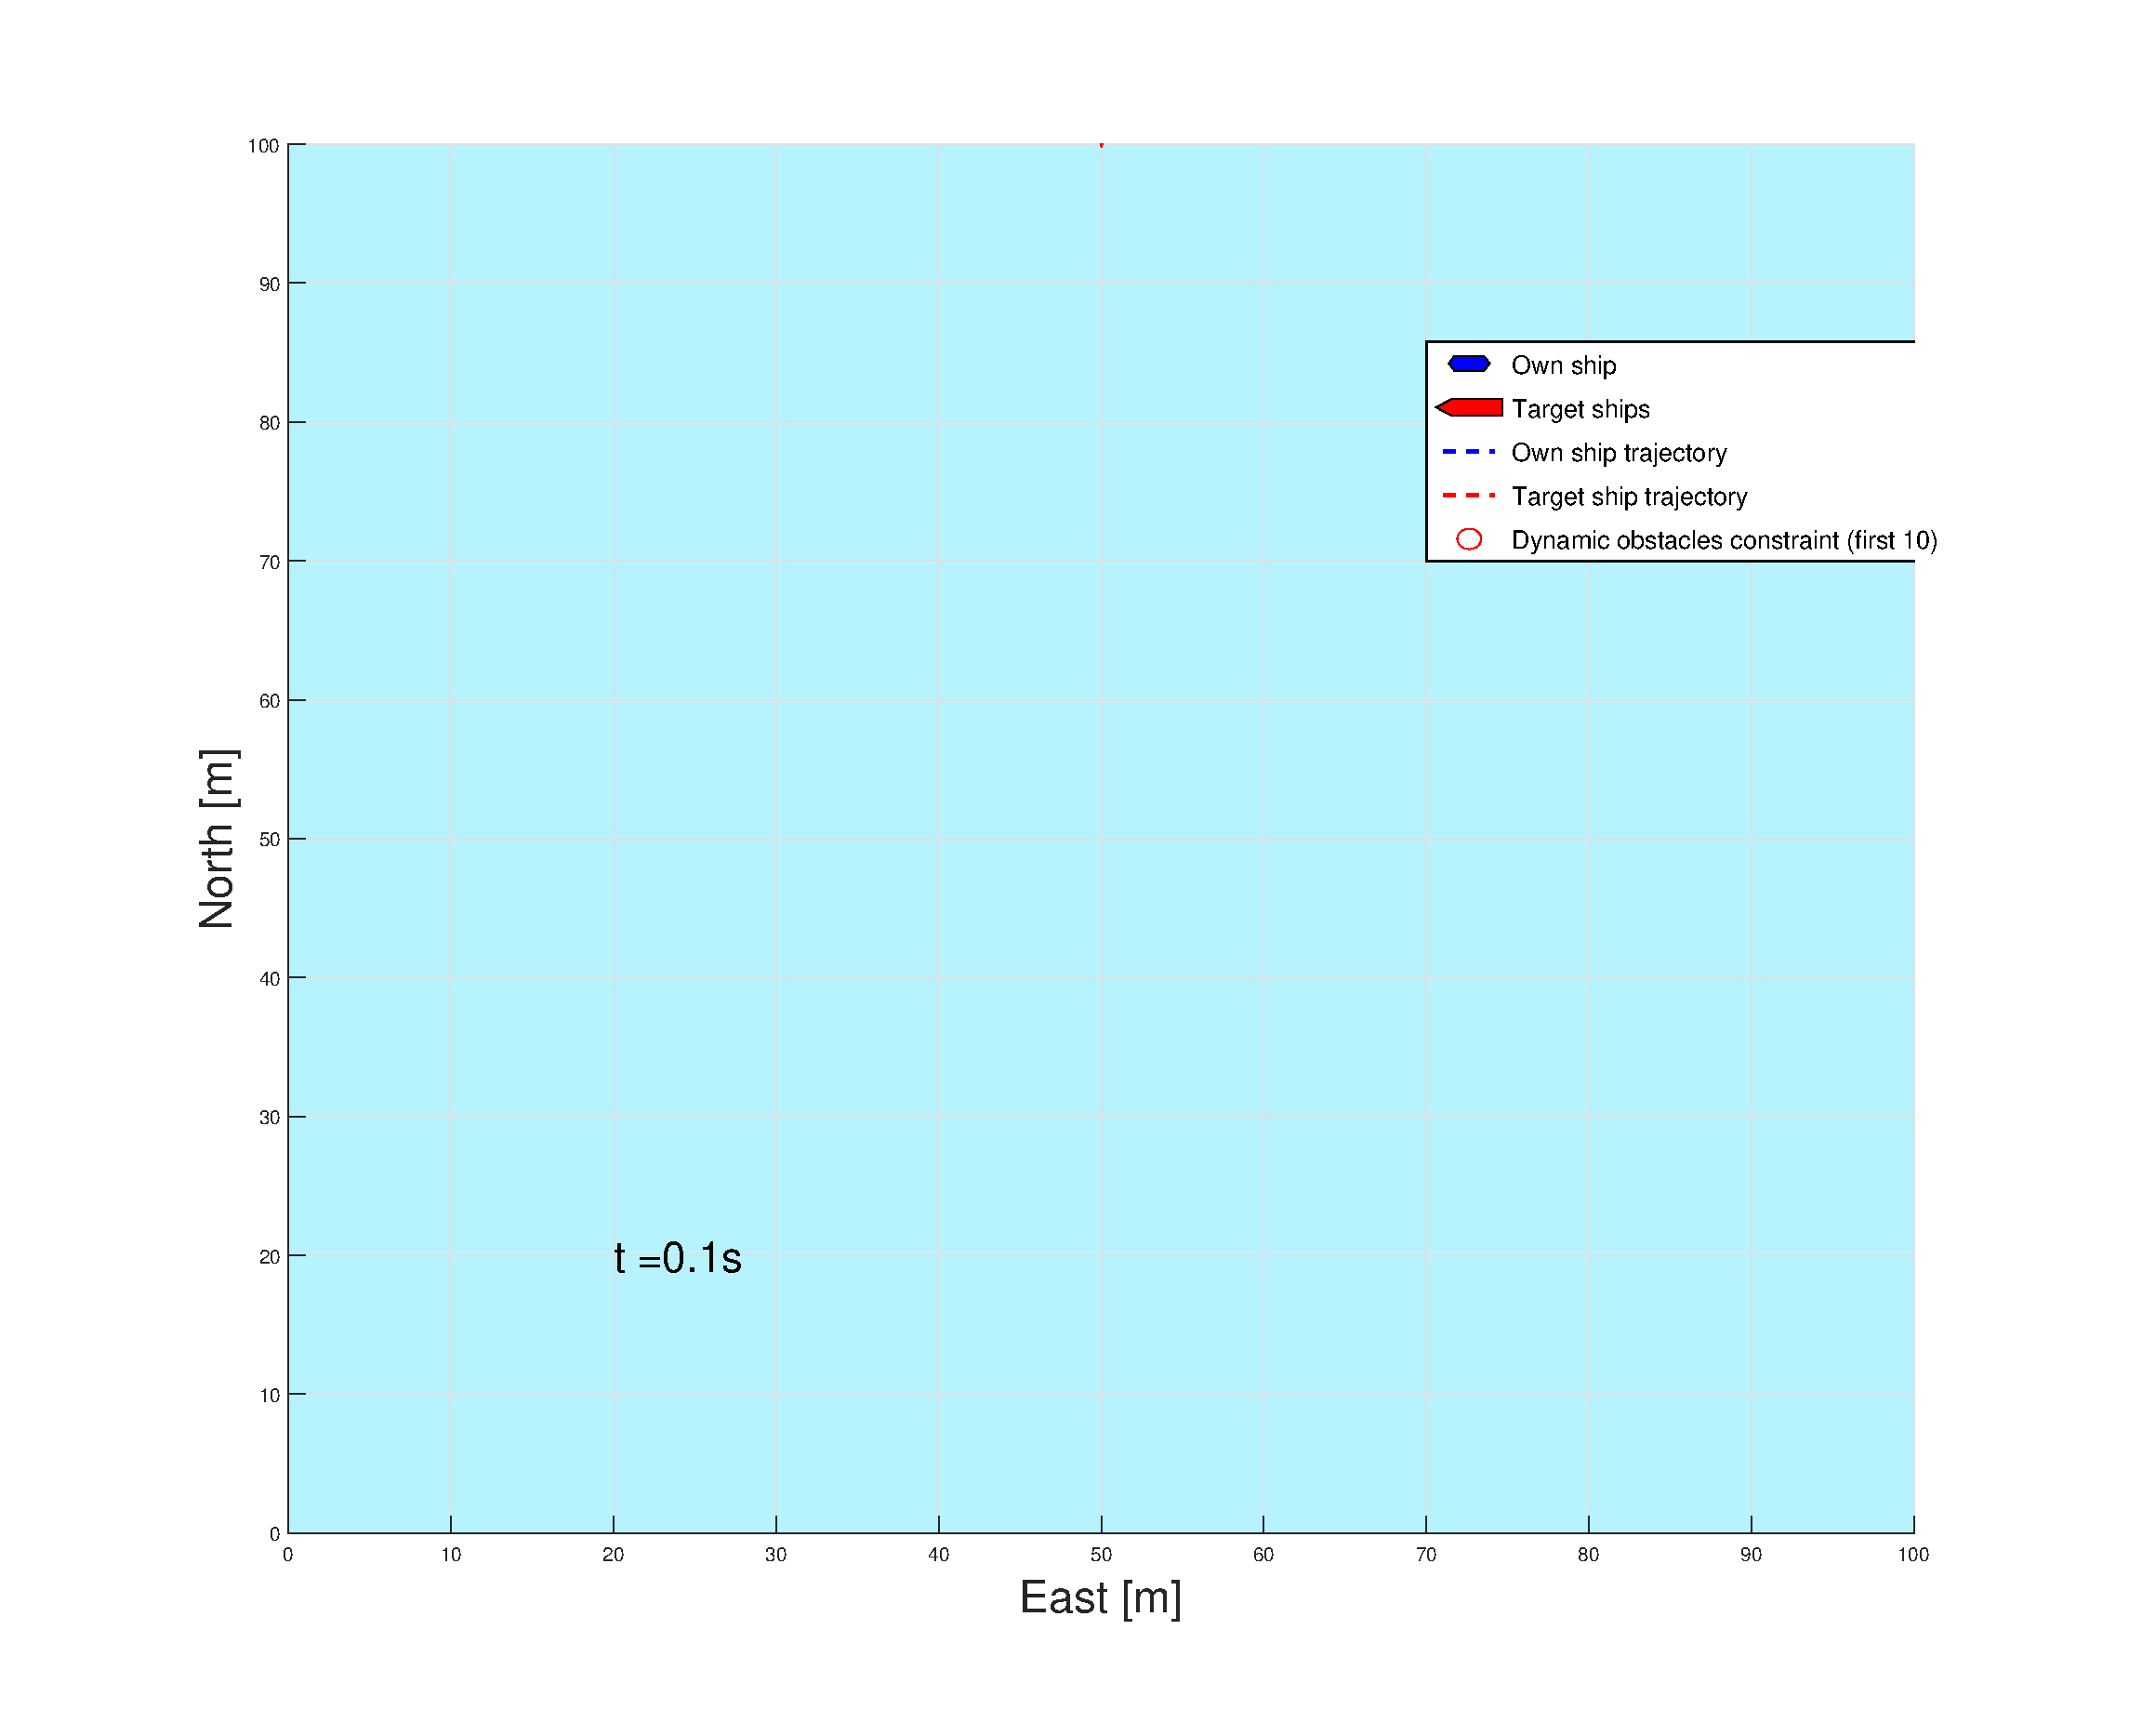
\includegraphics[width=\textwidth]{Images/Figures/enkel_HO/_Simple_0fig1_time=0}
    %     \subcaption{}
    % \end{subfigure}
    % \hfill
    % \begin{subfigure}[b]{0.499\textwidth}
    %     \centering
    %     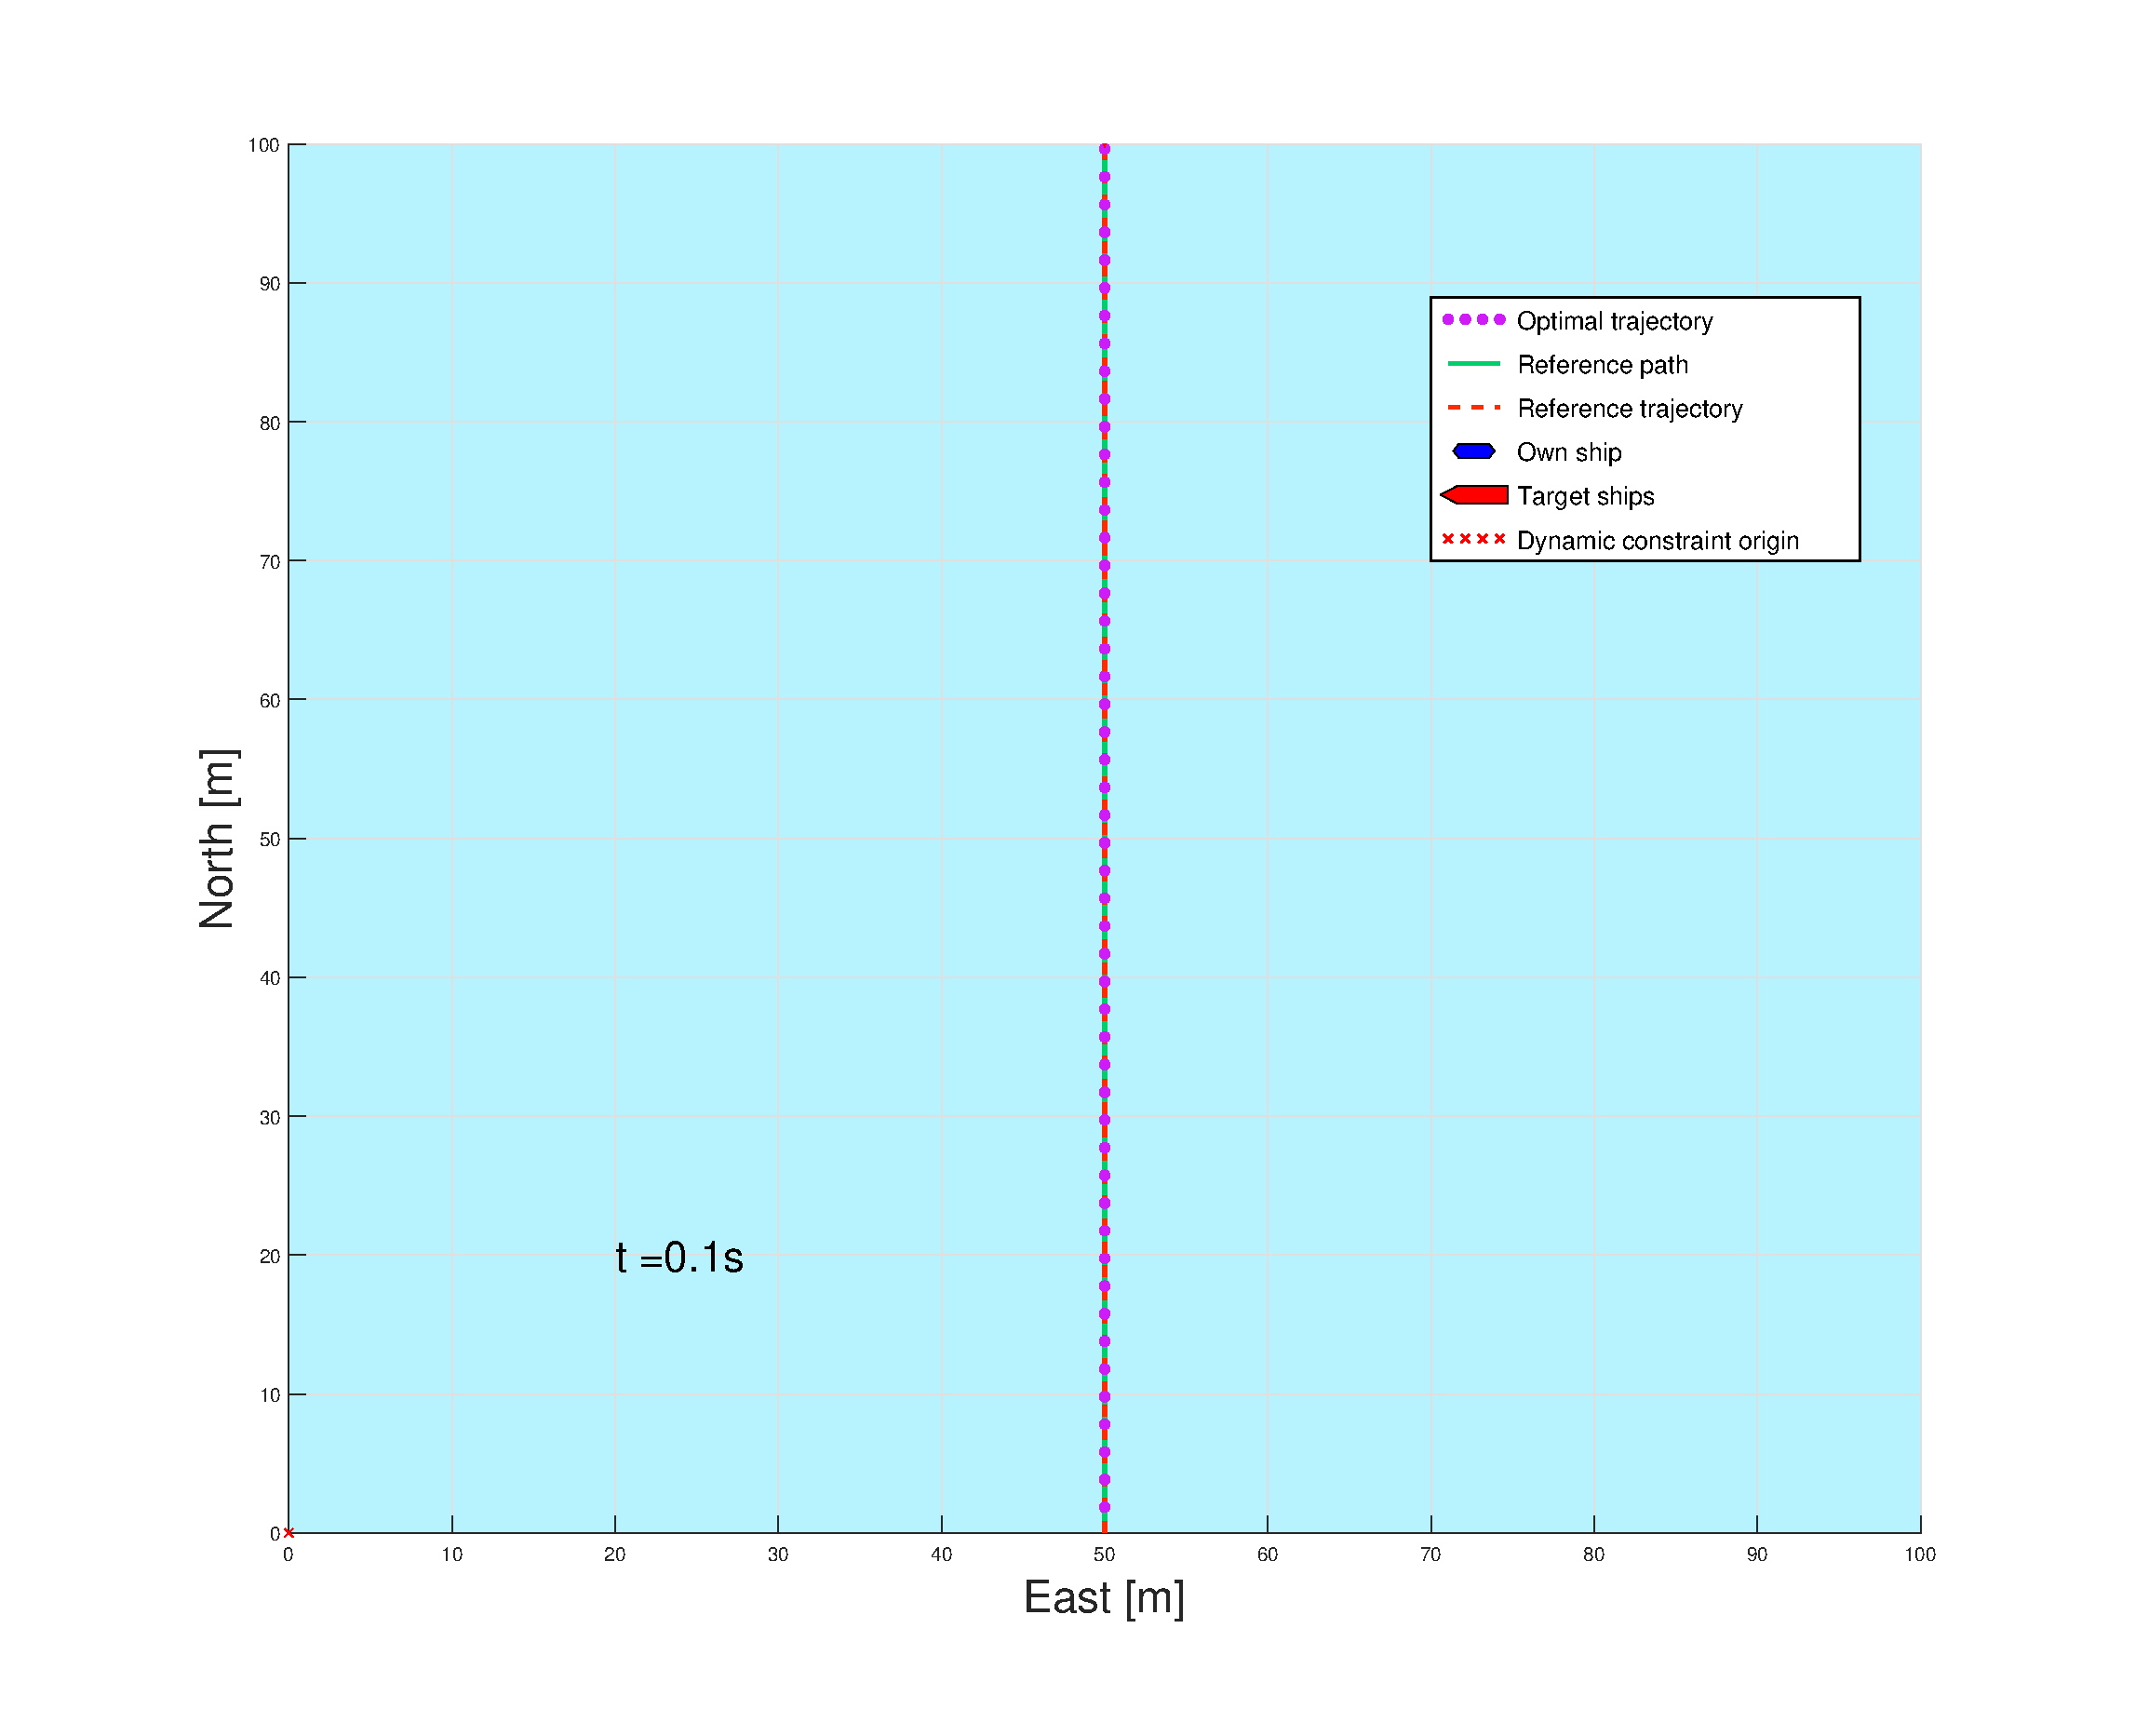
\includegraphics[width=\textwidth]{Images/Figures/enkel_HO/_Simple_0fig999_time=0}
    %     \subcaption{}
    % \end{subfigure}
    % \hfill
    % \\
    \begin{subfigure}[b]{0.49\textwidth}
        \centering
        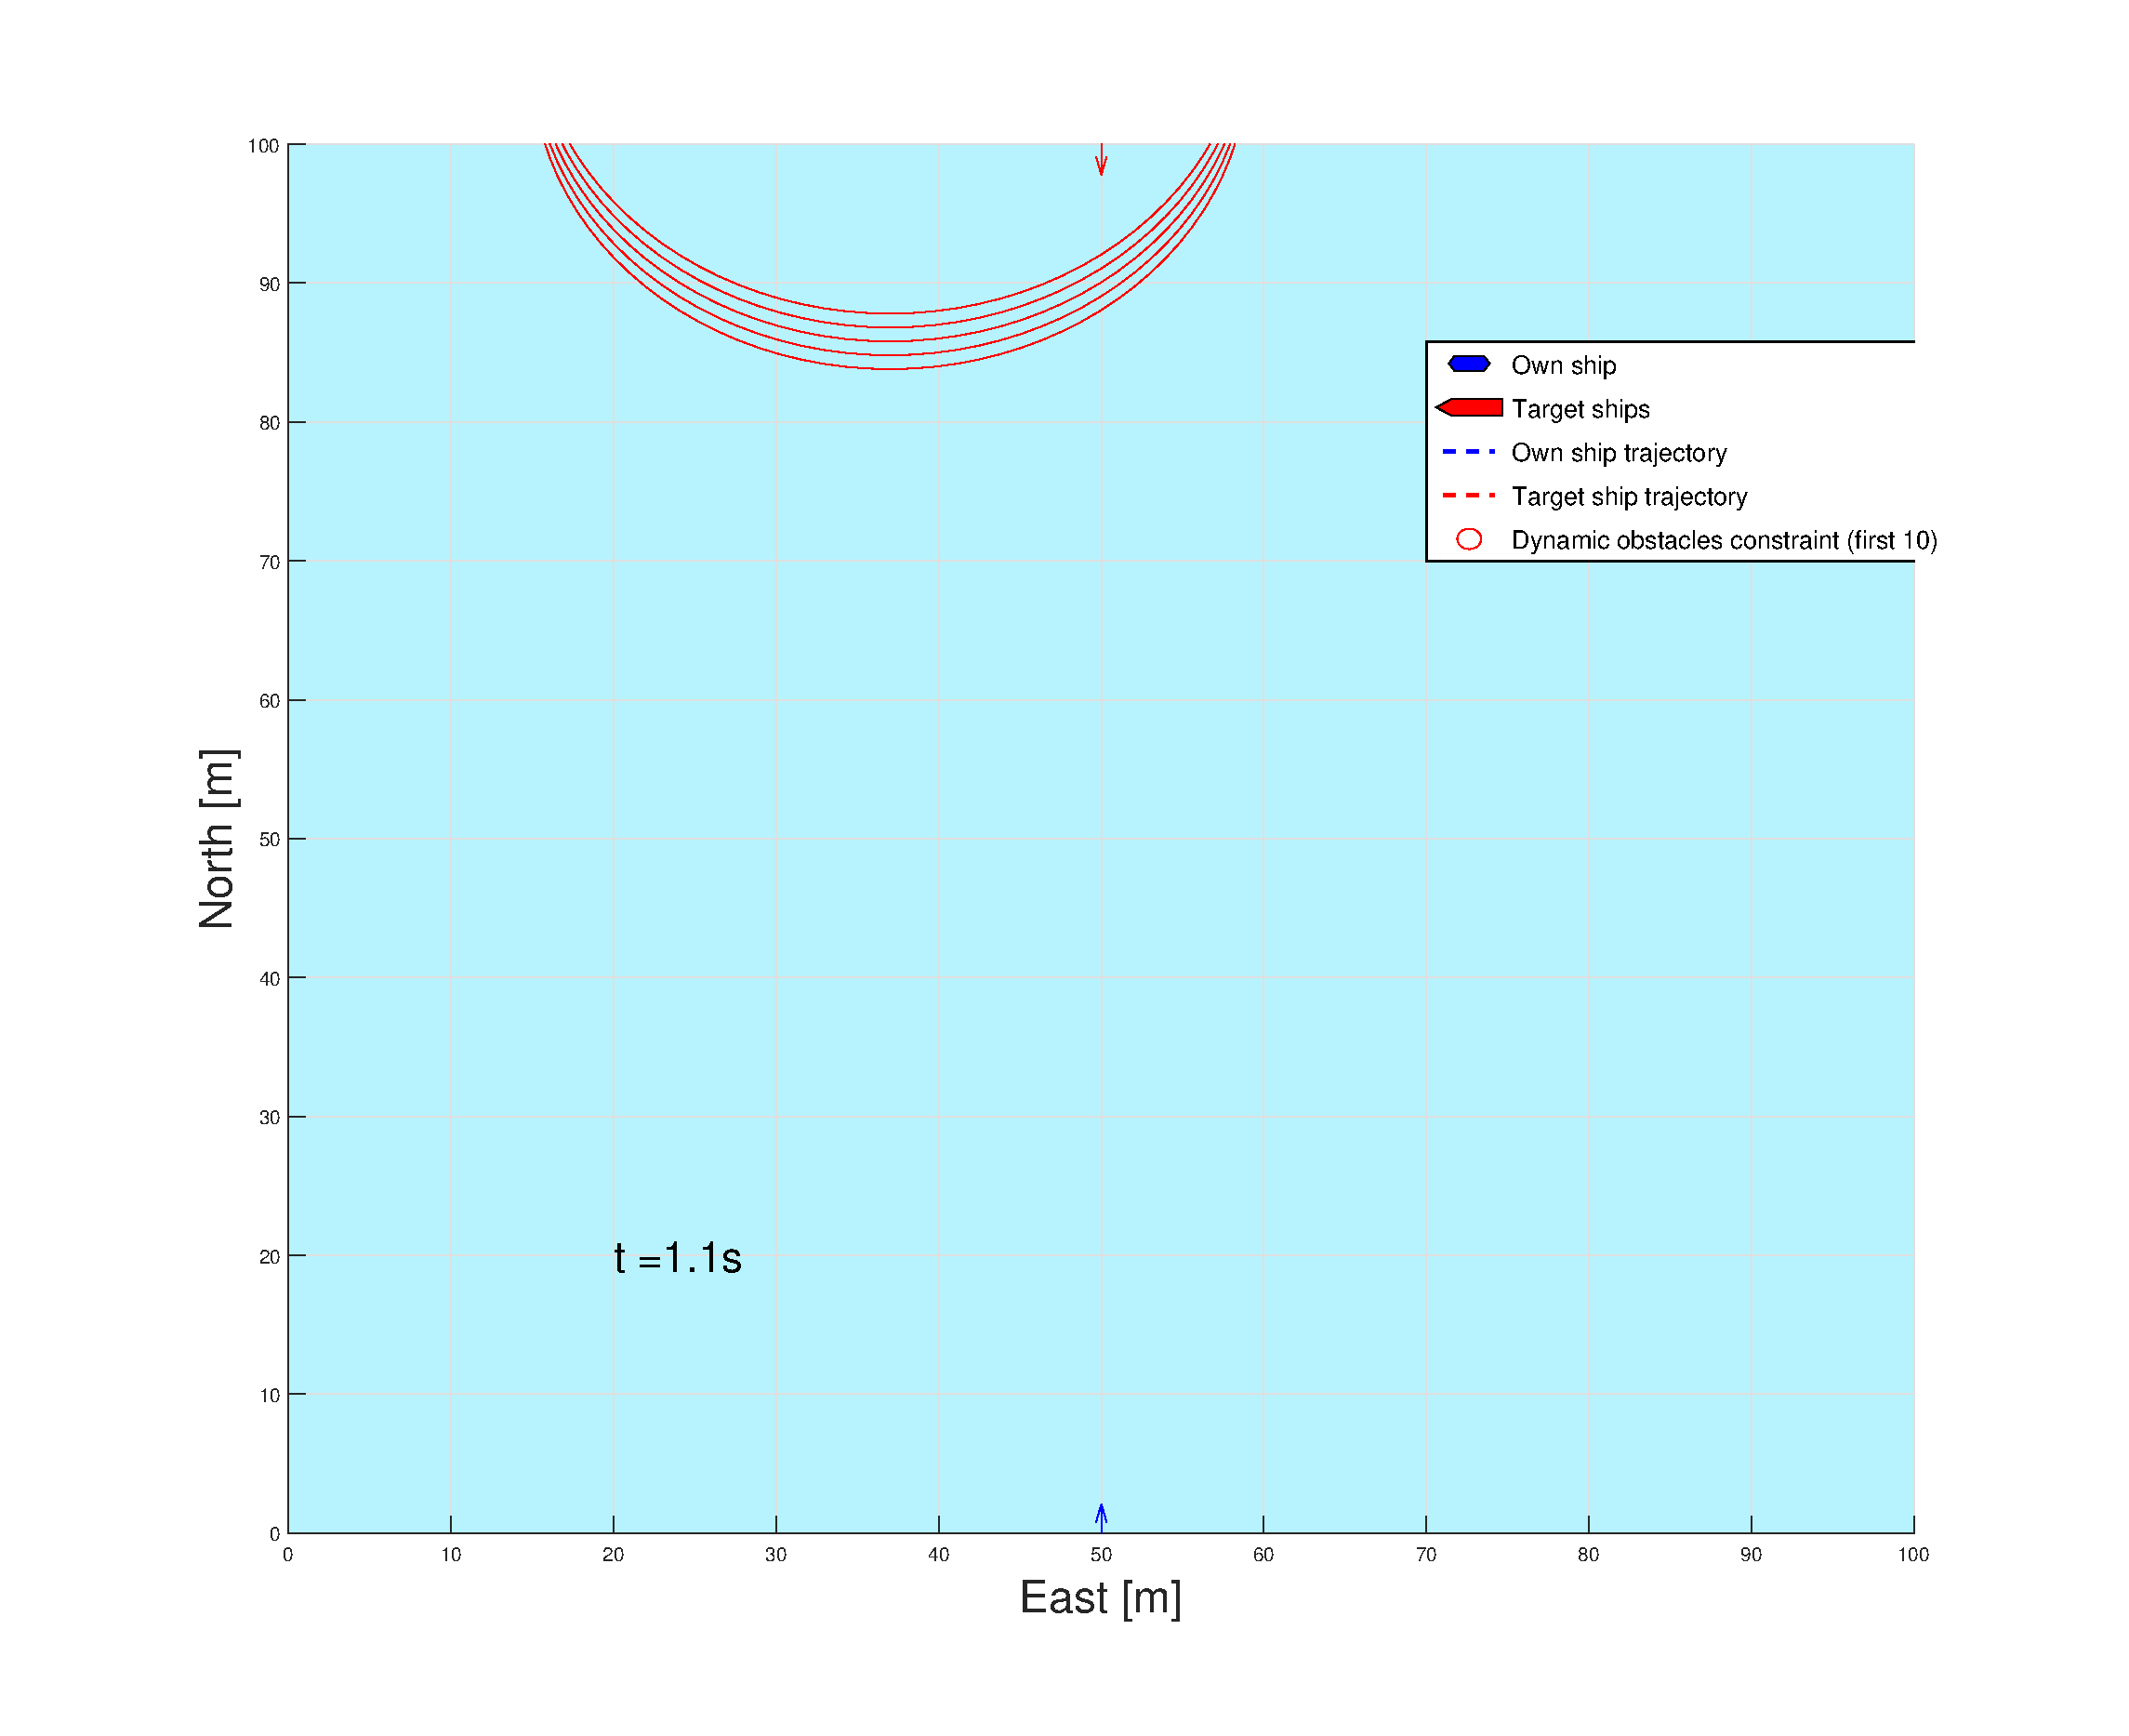
\includegraphics[width=\textwidth]{Images/Figures/enkel_HO/_Simple_0fig1_time=1}
        \subcaption{}
    \end{subfigure}
    \hfill
    \begin{subfigure}[b]{0.499\textwidth}
        \centering
        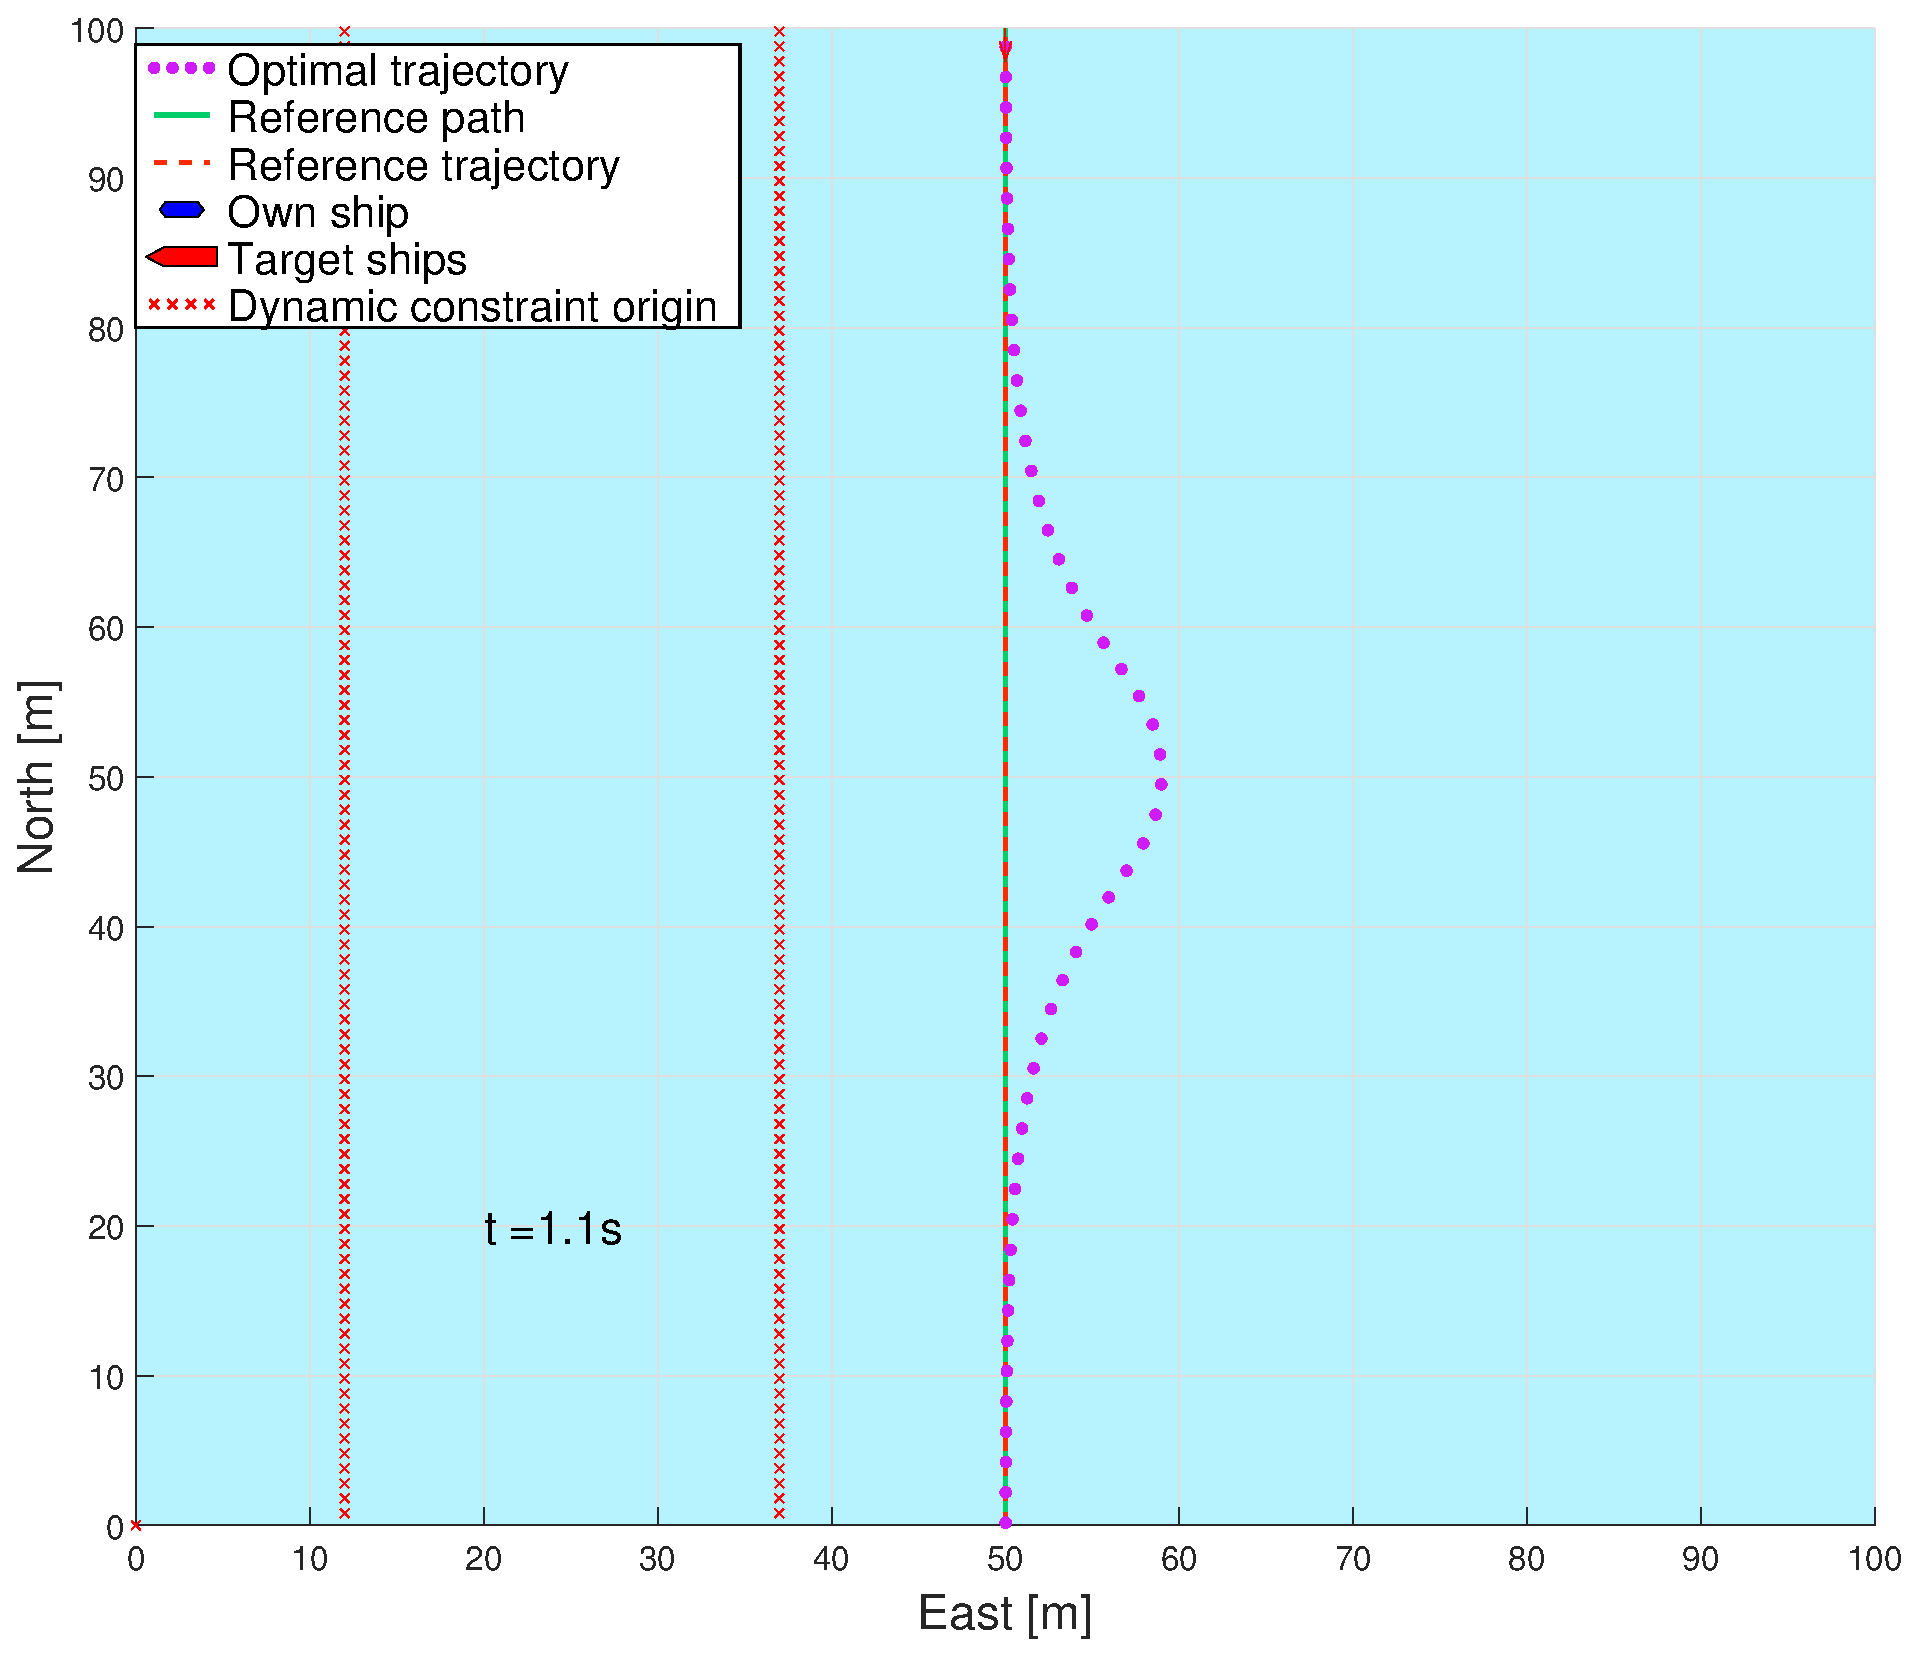
\includegraphics[width=\textwidth]{Images/Figures/enkel_HO/_Simple_0fig999_time=1}
        \subcaption{}
    \end{subfigure}
    \hfill
    \\
    \begin{subfigure}[b]{0.49\textwidth}
        \centering
        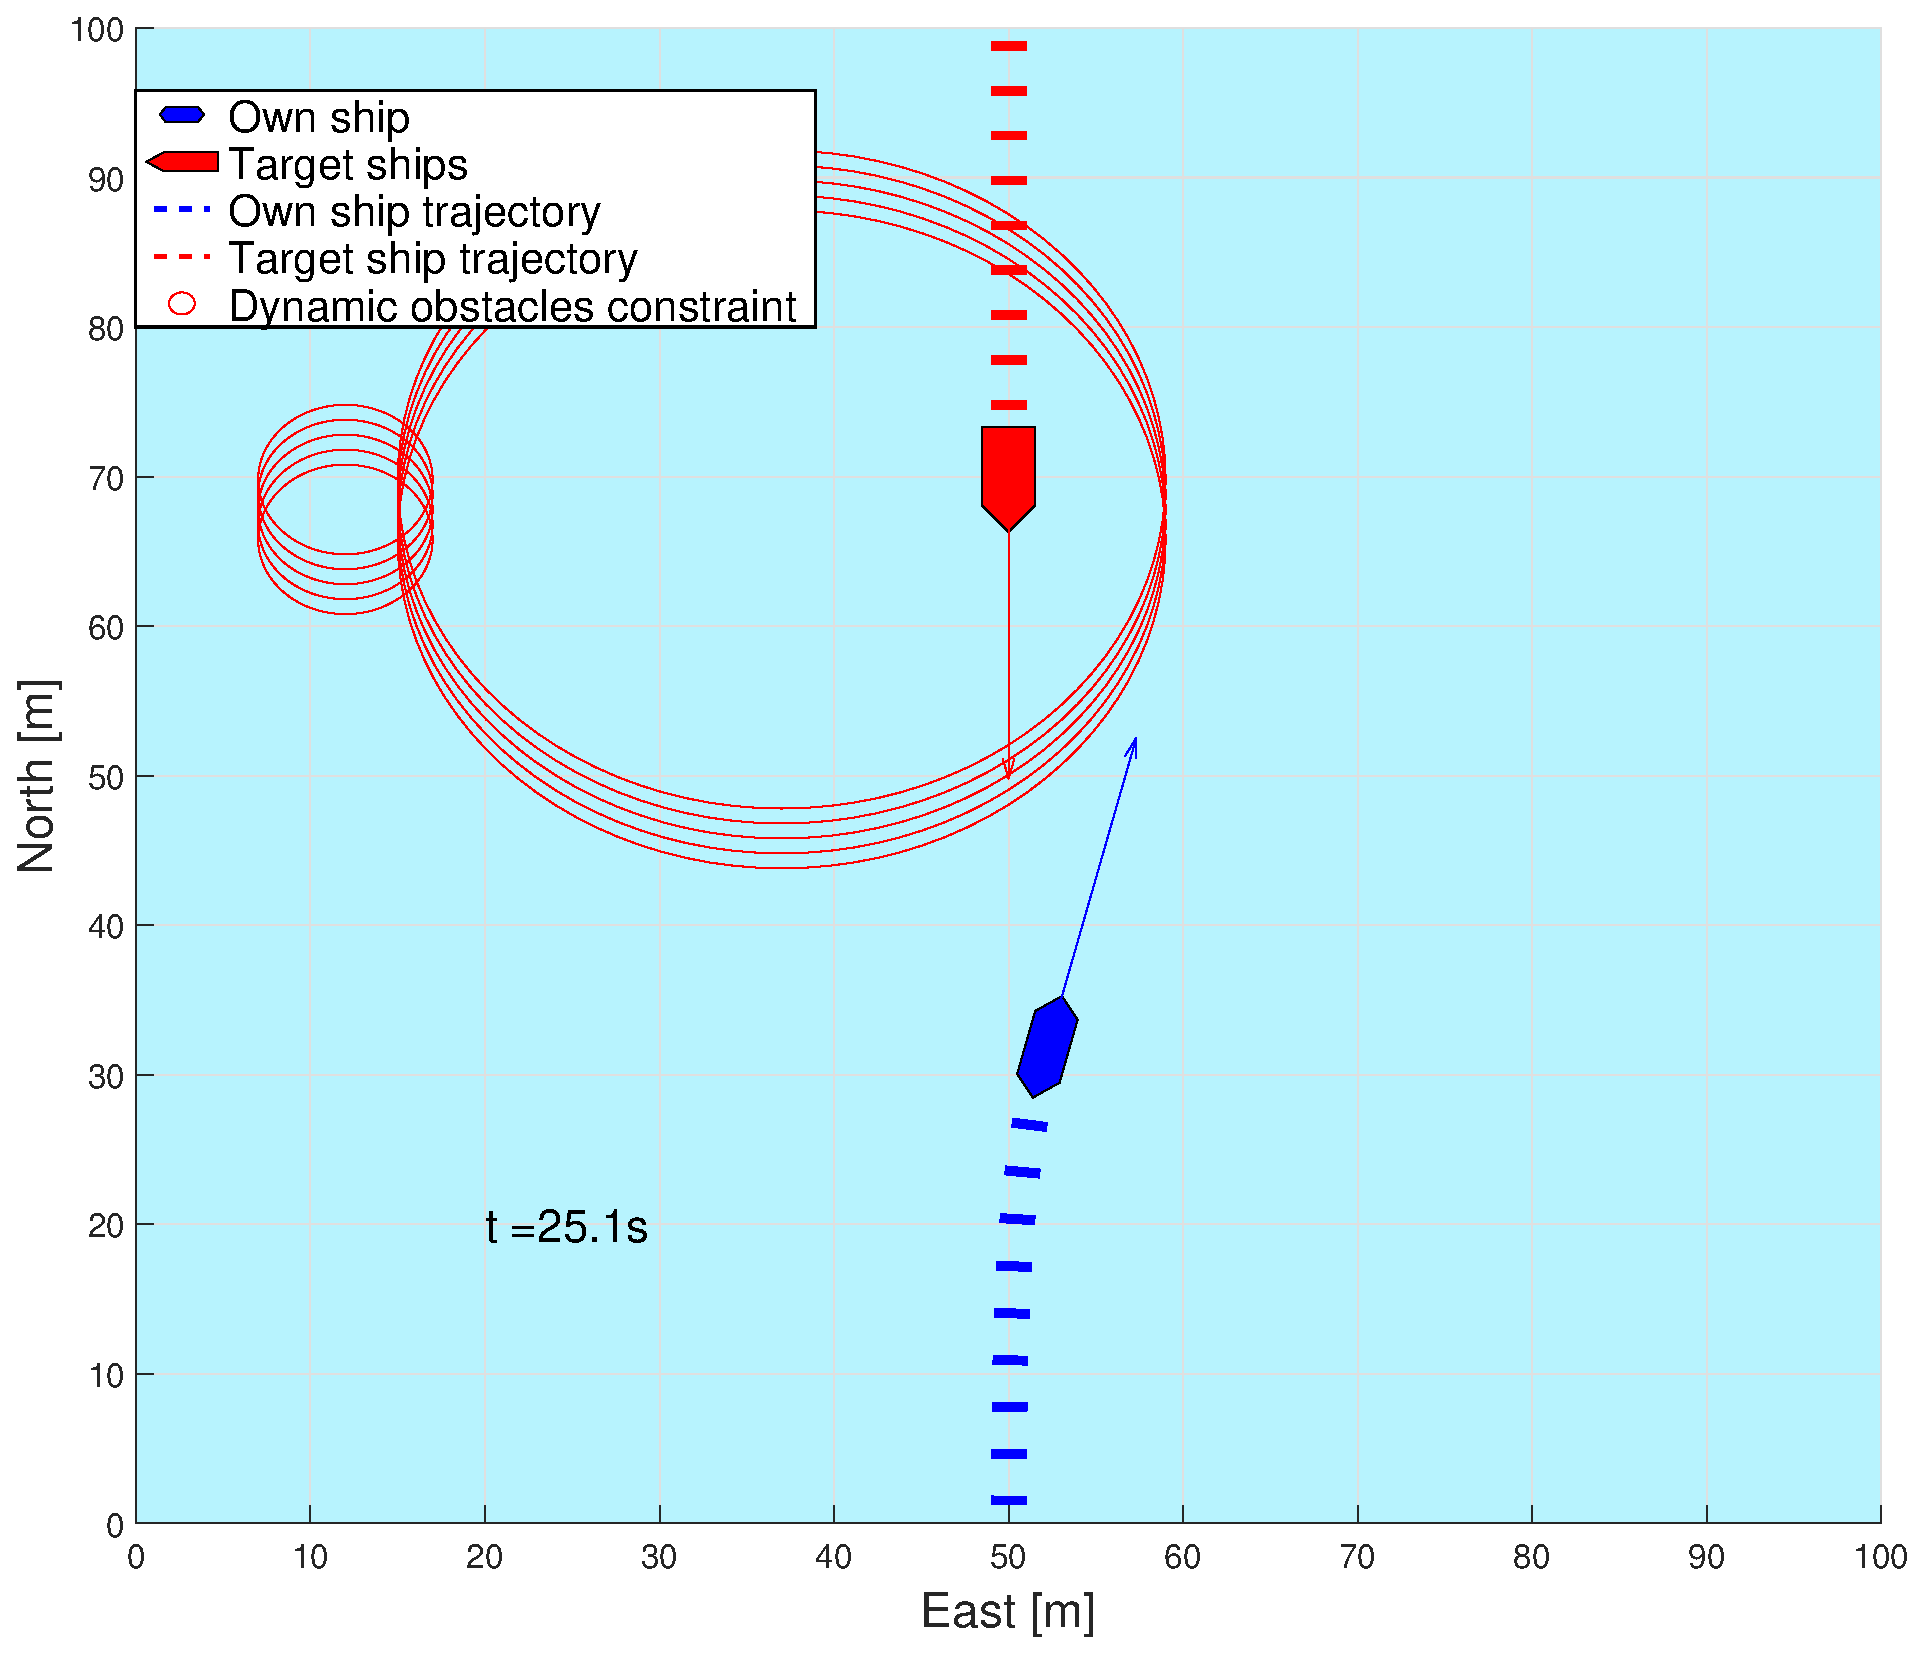
\includegraphics[width=\textwidth]{Images/Figures/enkel_HO/_Simple_0fig1_time=25}
        \subcaption{}
    \end{subfigure}
    \hfill
    \begin{subfigure}[b]{0.499\textwidth}
        \centering
        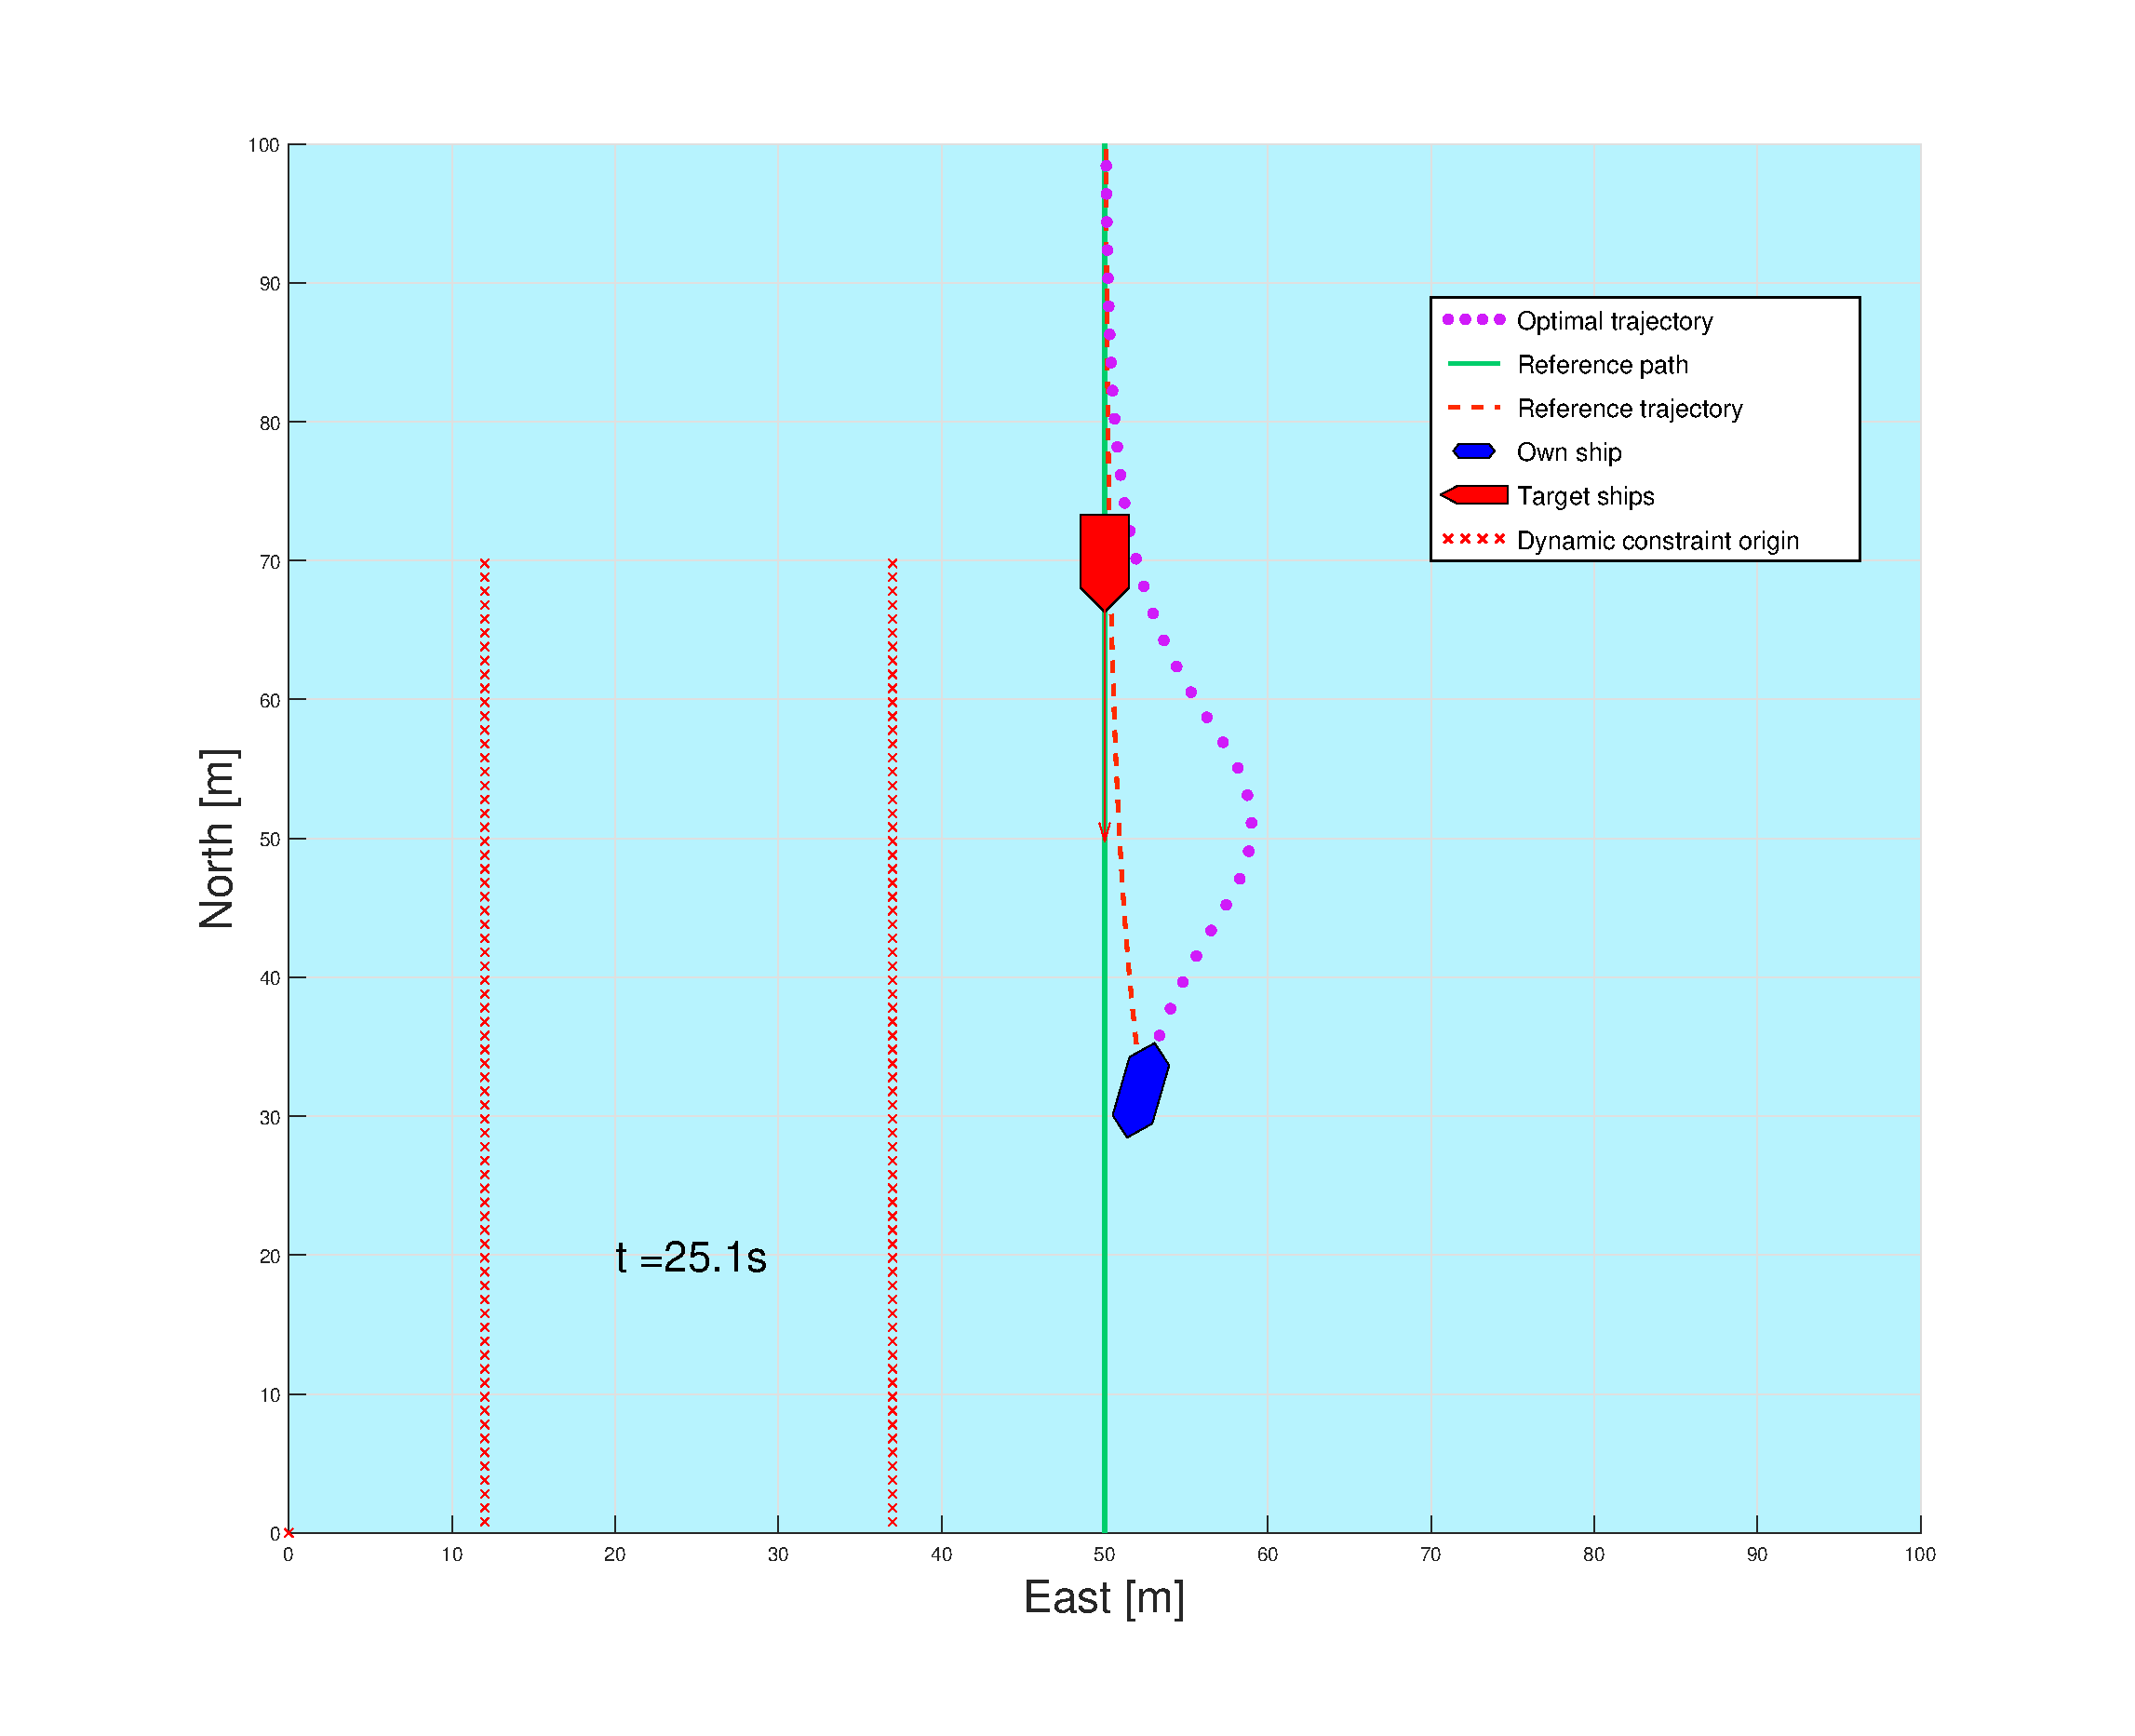
\includegraphics[width=\textwidth]{Images/Figures/enkel_HO/_Simple_0fig999_time=25}
        \subcaption{}
    \end{subfigure}
    \hfill
    \\
    \begin{subfigure}[b]{0.49\textwidth}
        \centering
        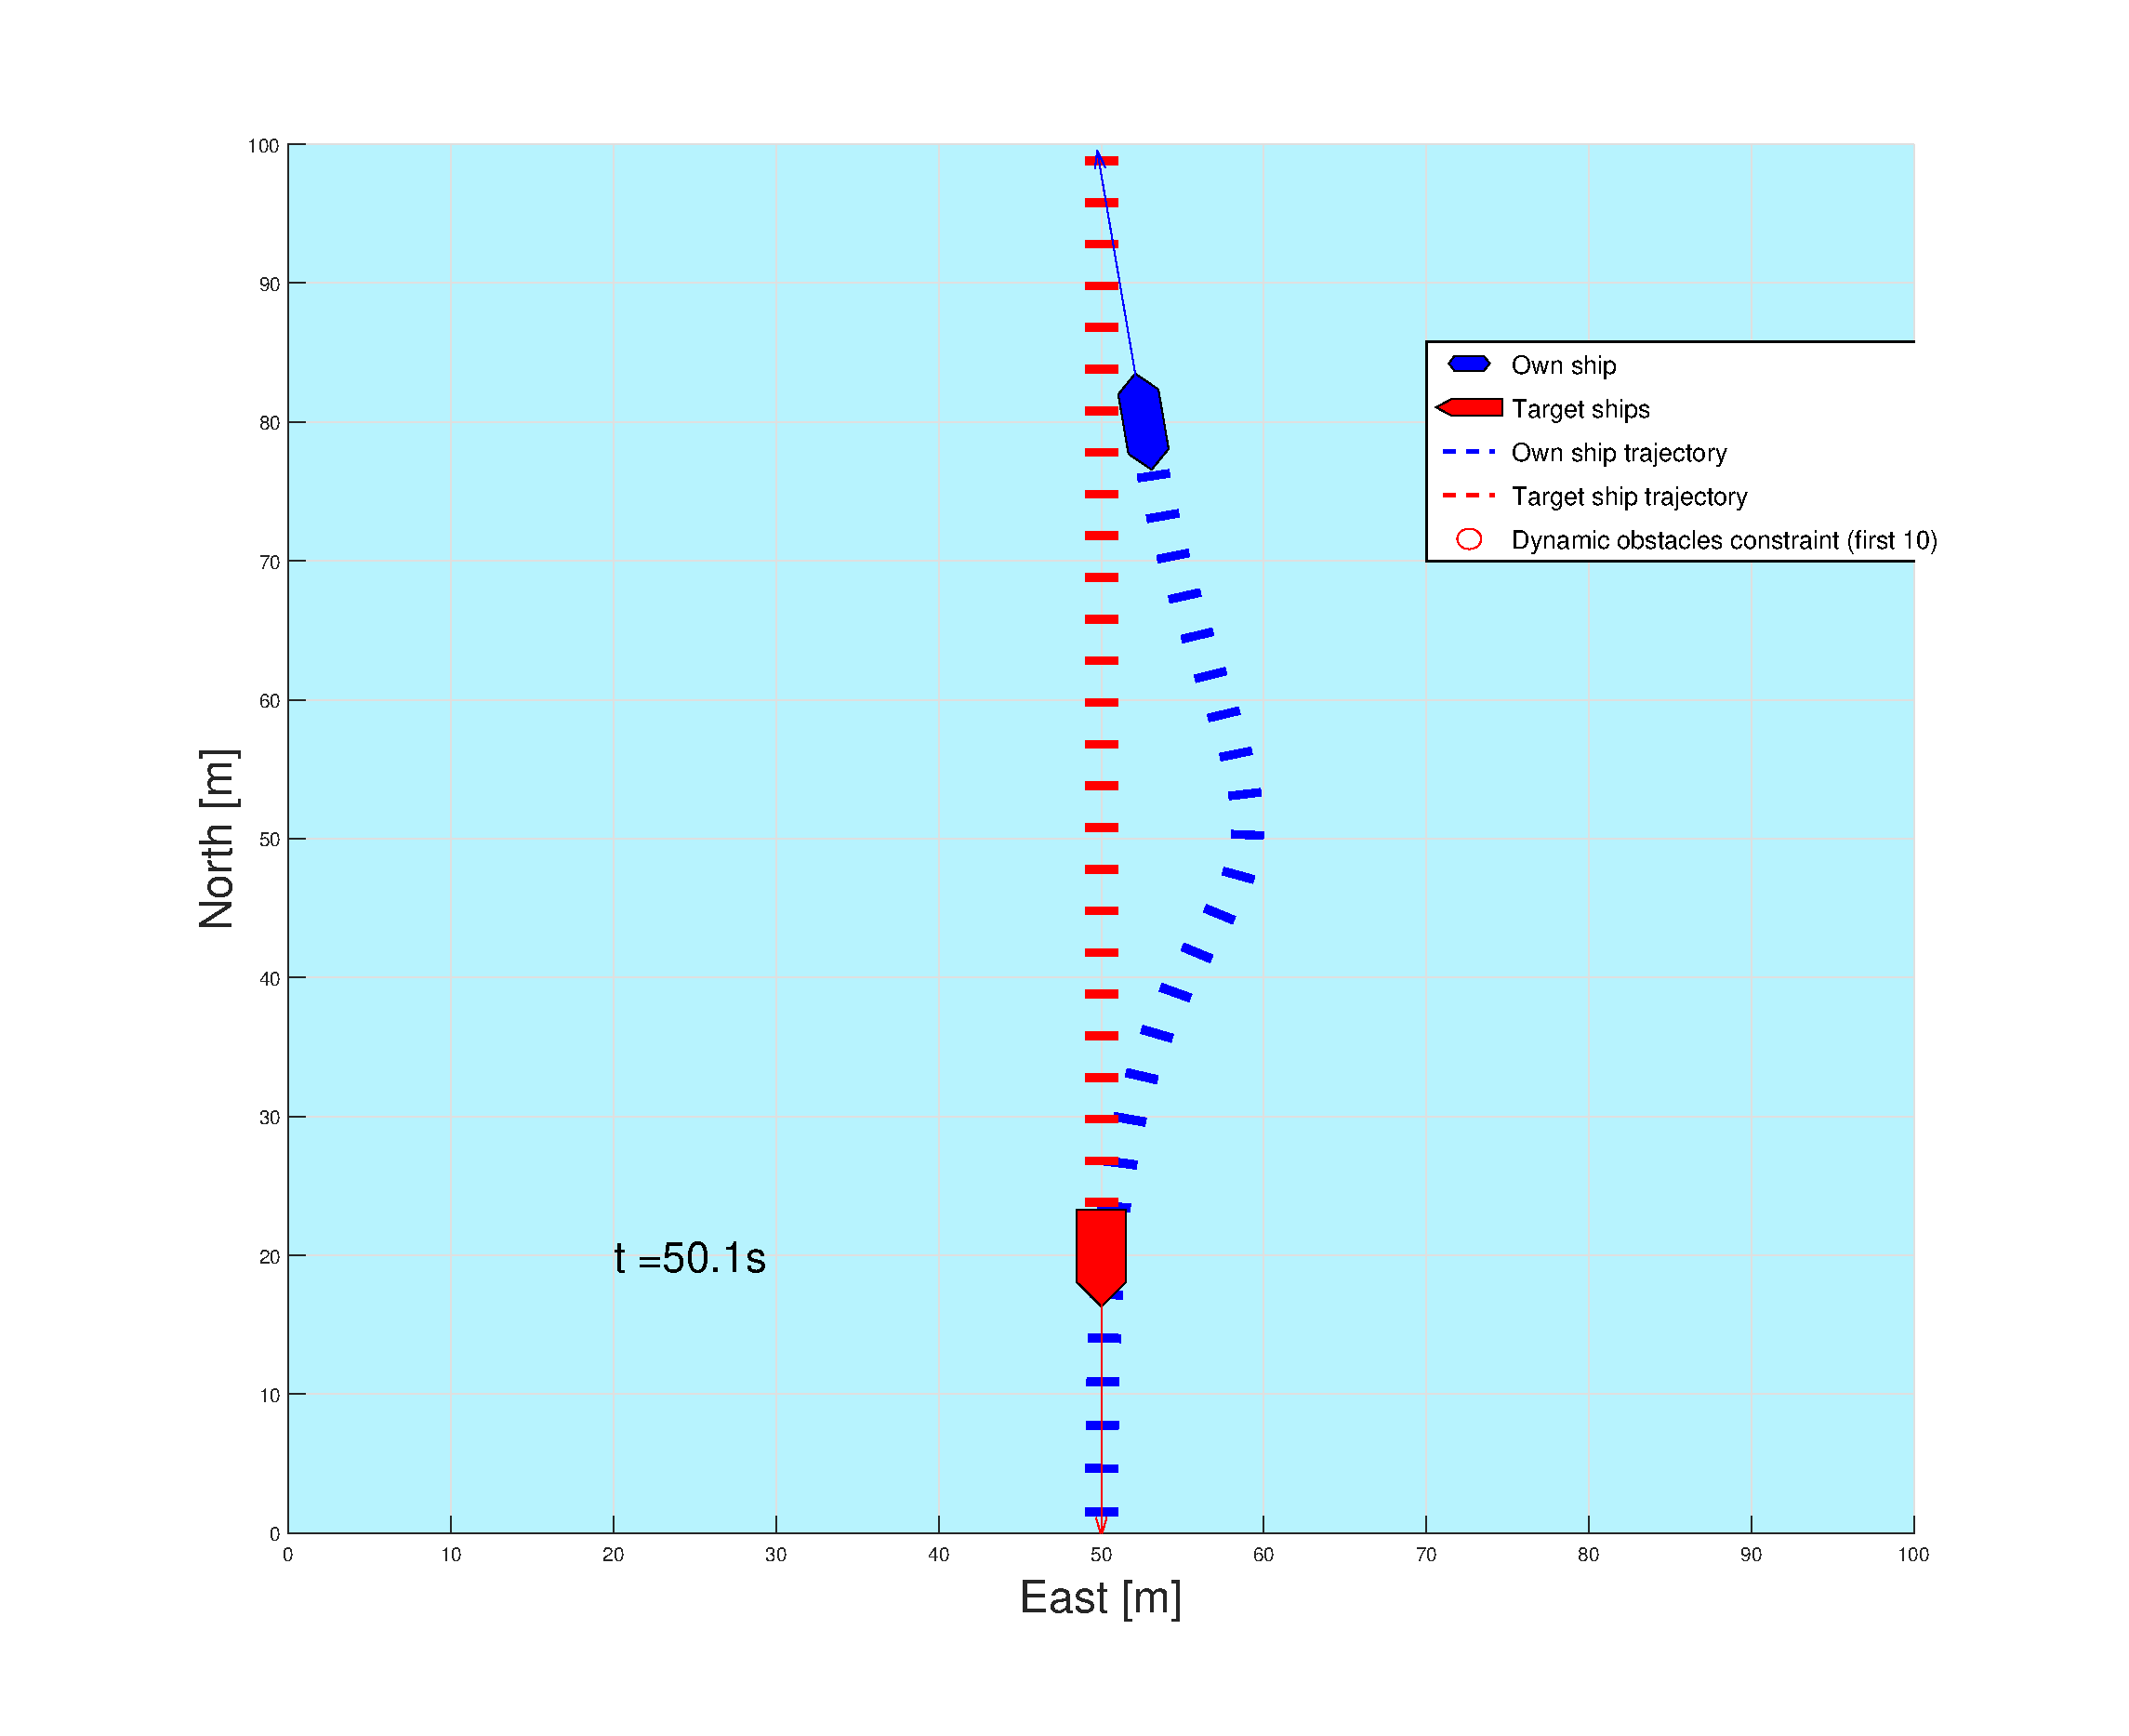
\includegraphics[width=\textwidth]{Images/Figures/enkel_HO/_Simple_0fig1_time=50}
        \subcaption{}
    \end{subfigure}
    \hfill
    \begin{subfigure}[b]{0.499\textwidth}
        \centering
        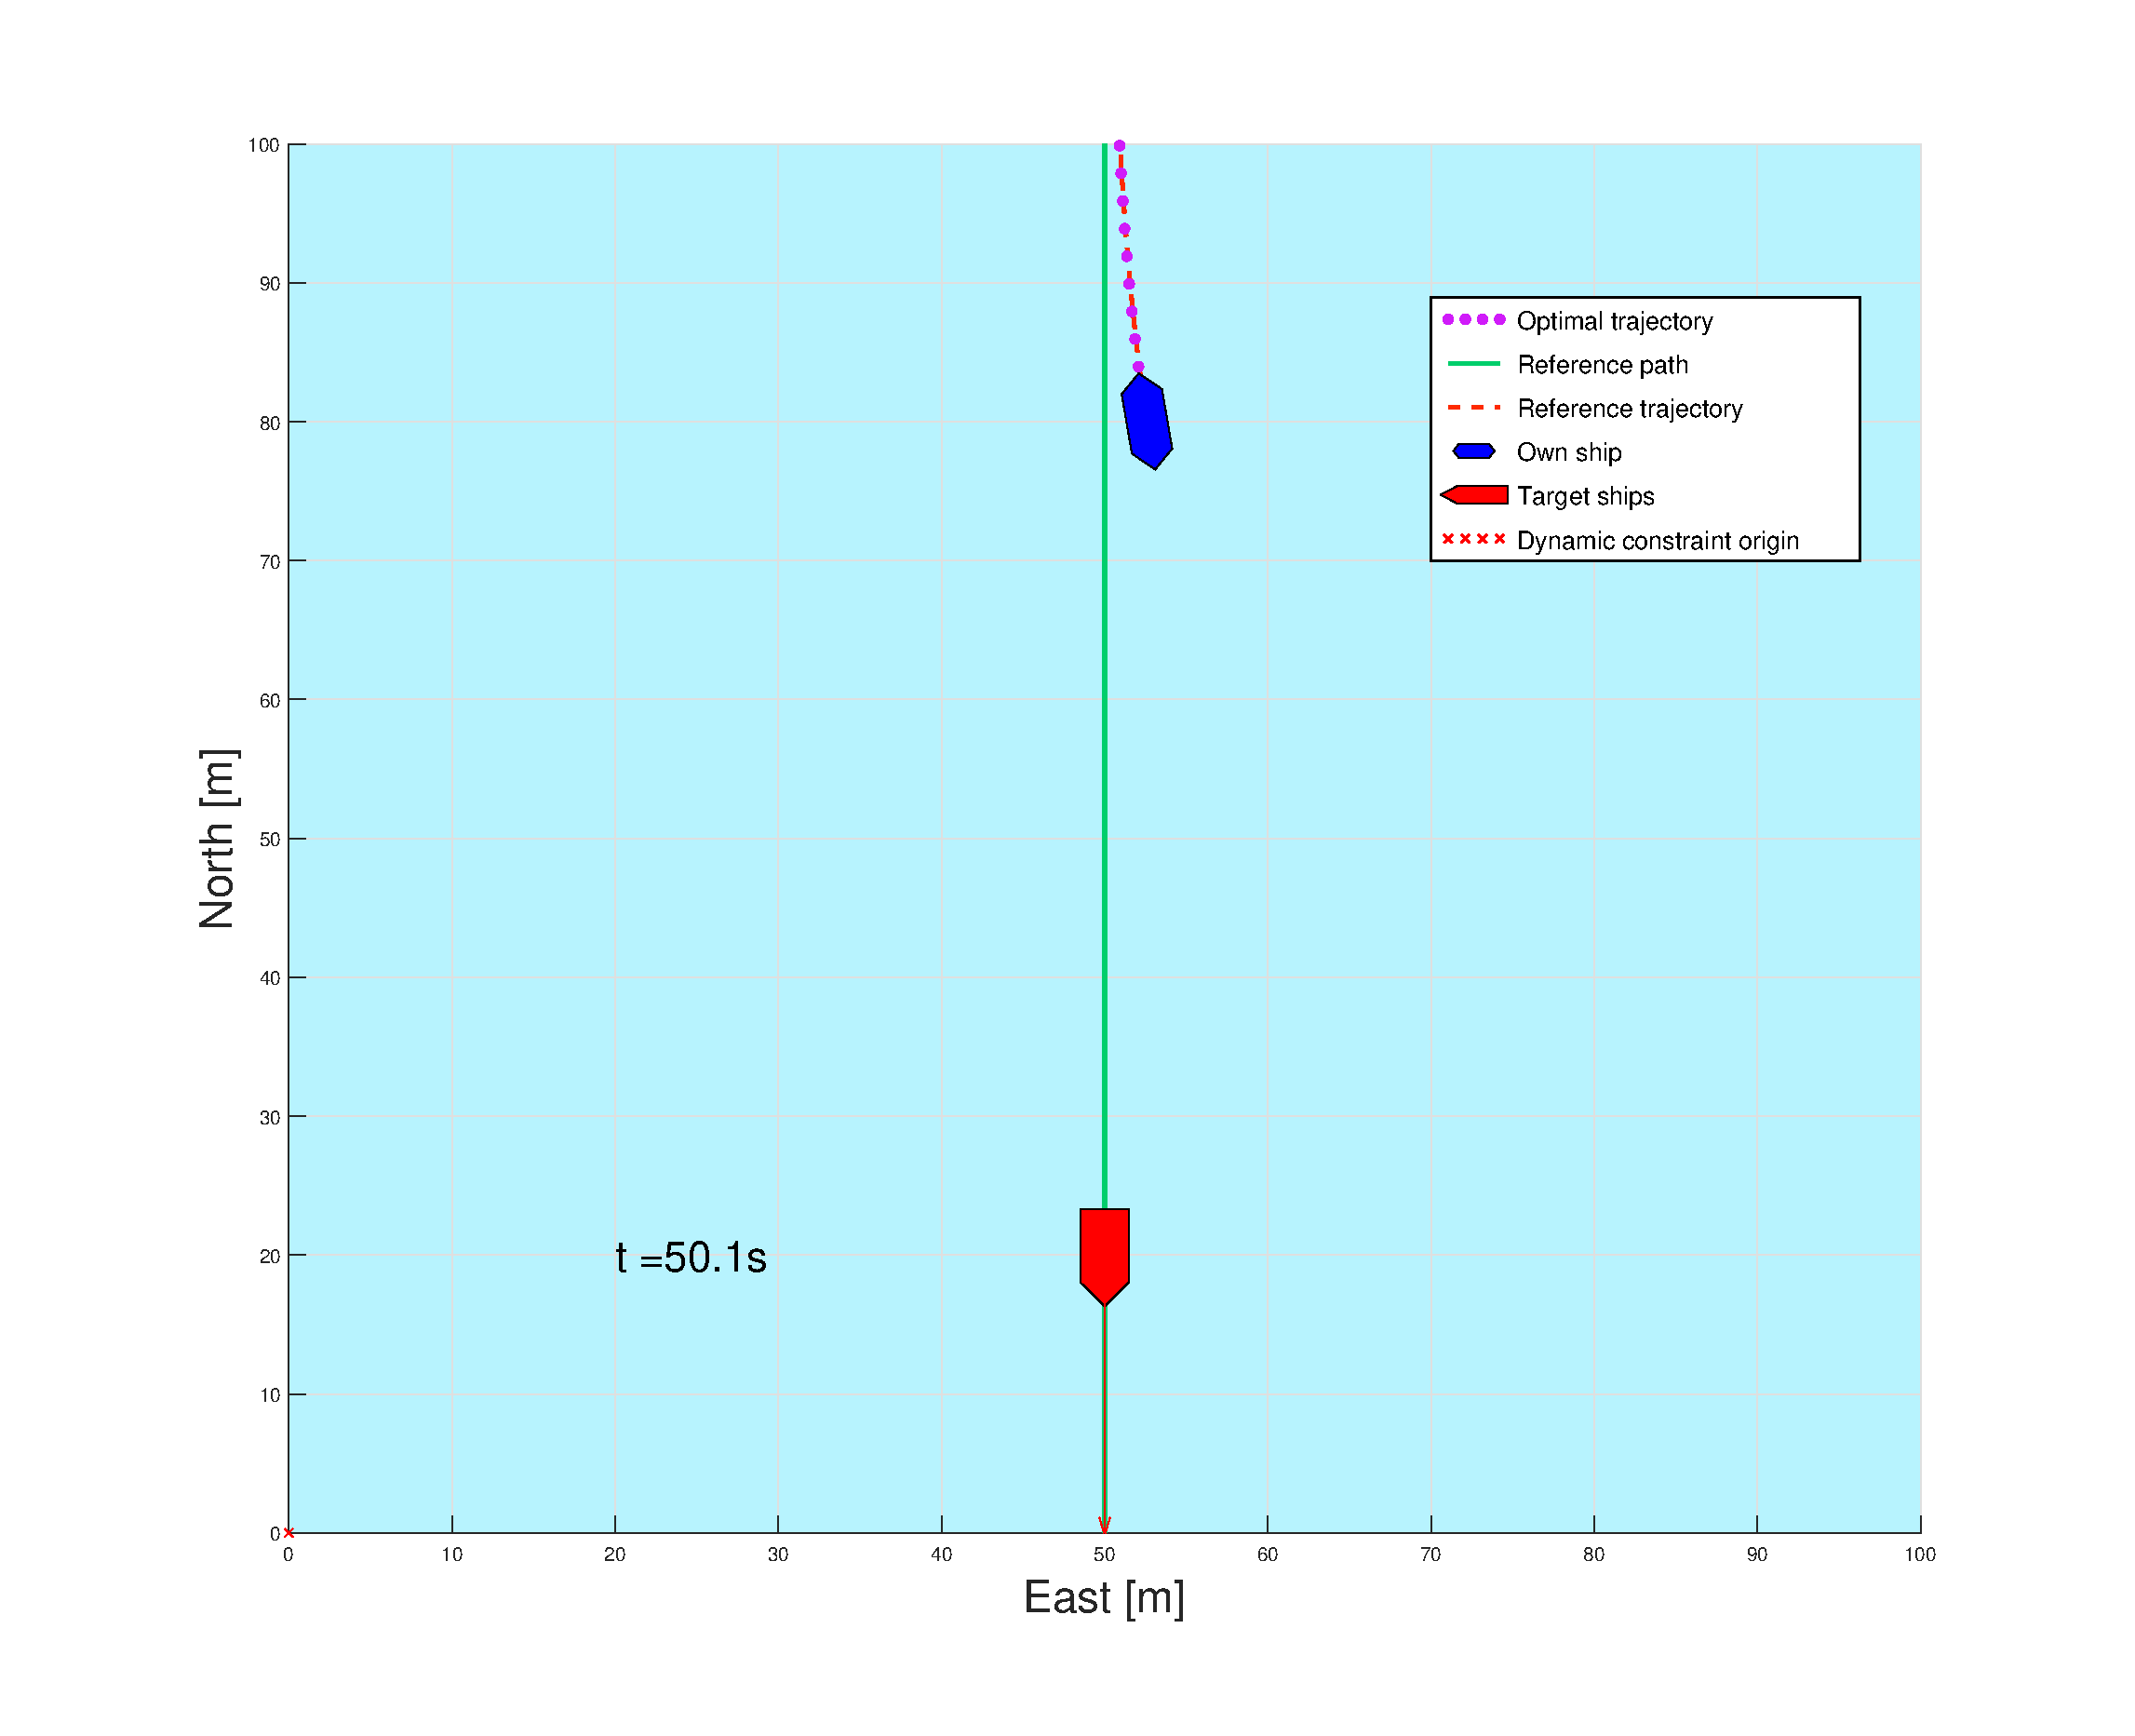
\includegraphics[width=\textwidth]{Images/Figures/enkel_HO/_Simple_0fig999_time=50}
        \subcaption{}
    \end{subfigure}
    \hfill
    \caption{Simple Head on situation. Result independent of prediction level.}
    \label{FIG: Simple HO}
\end{figure}%
% \begin{figure}[ht]\ContinuedFloat
%     \begin{subfigure}[b]{0.49\textwidth}
%         \centering
%         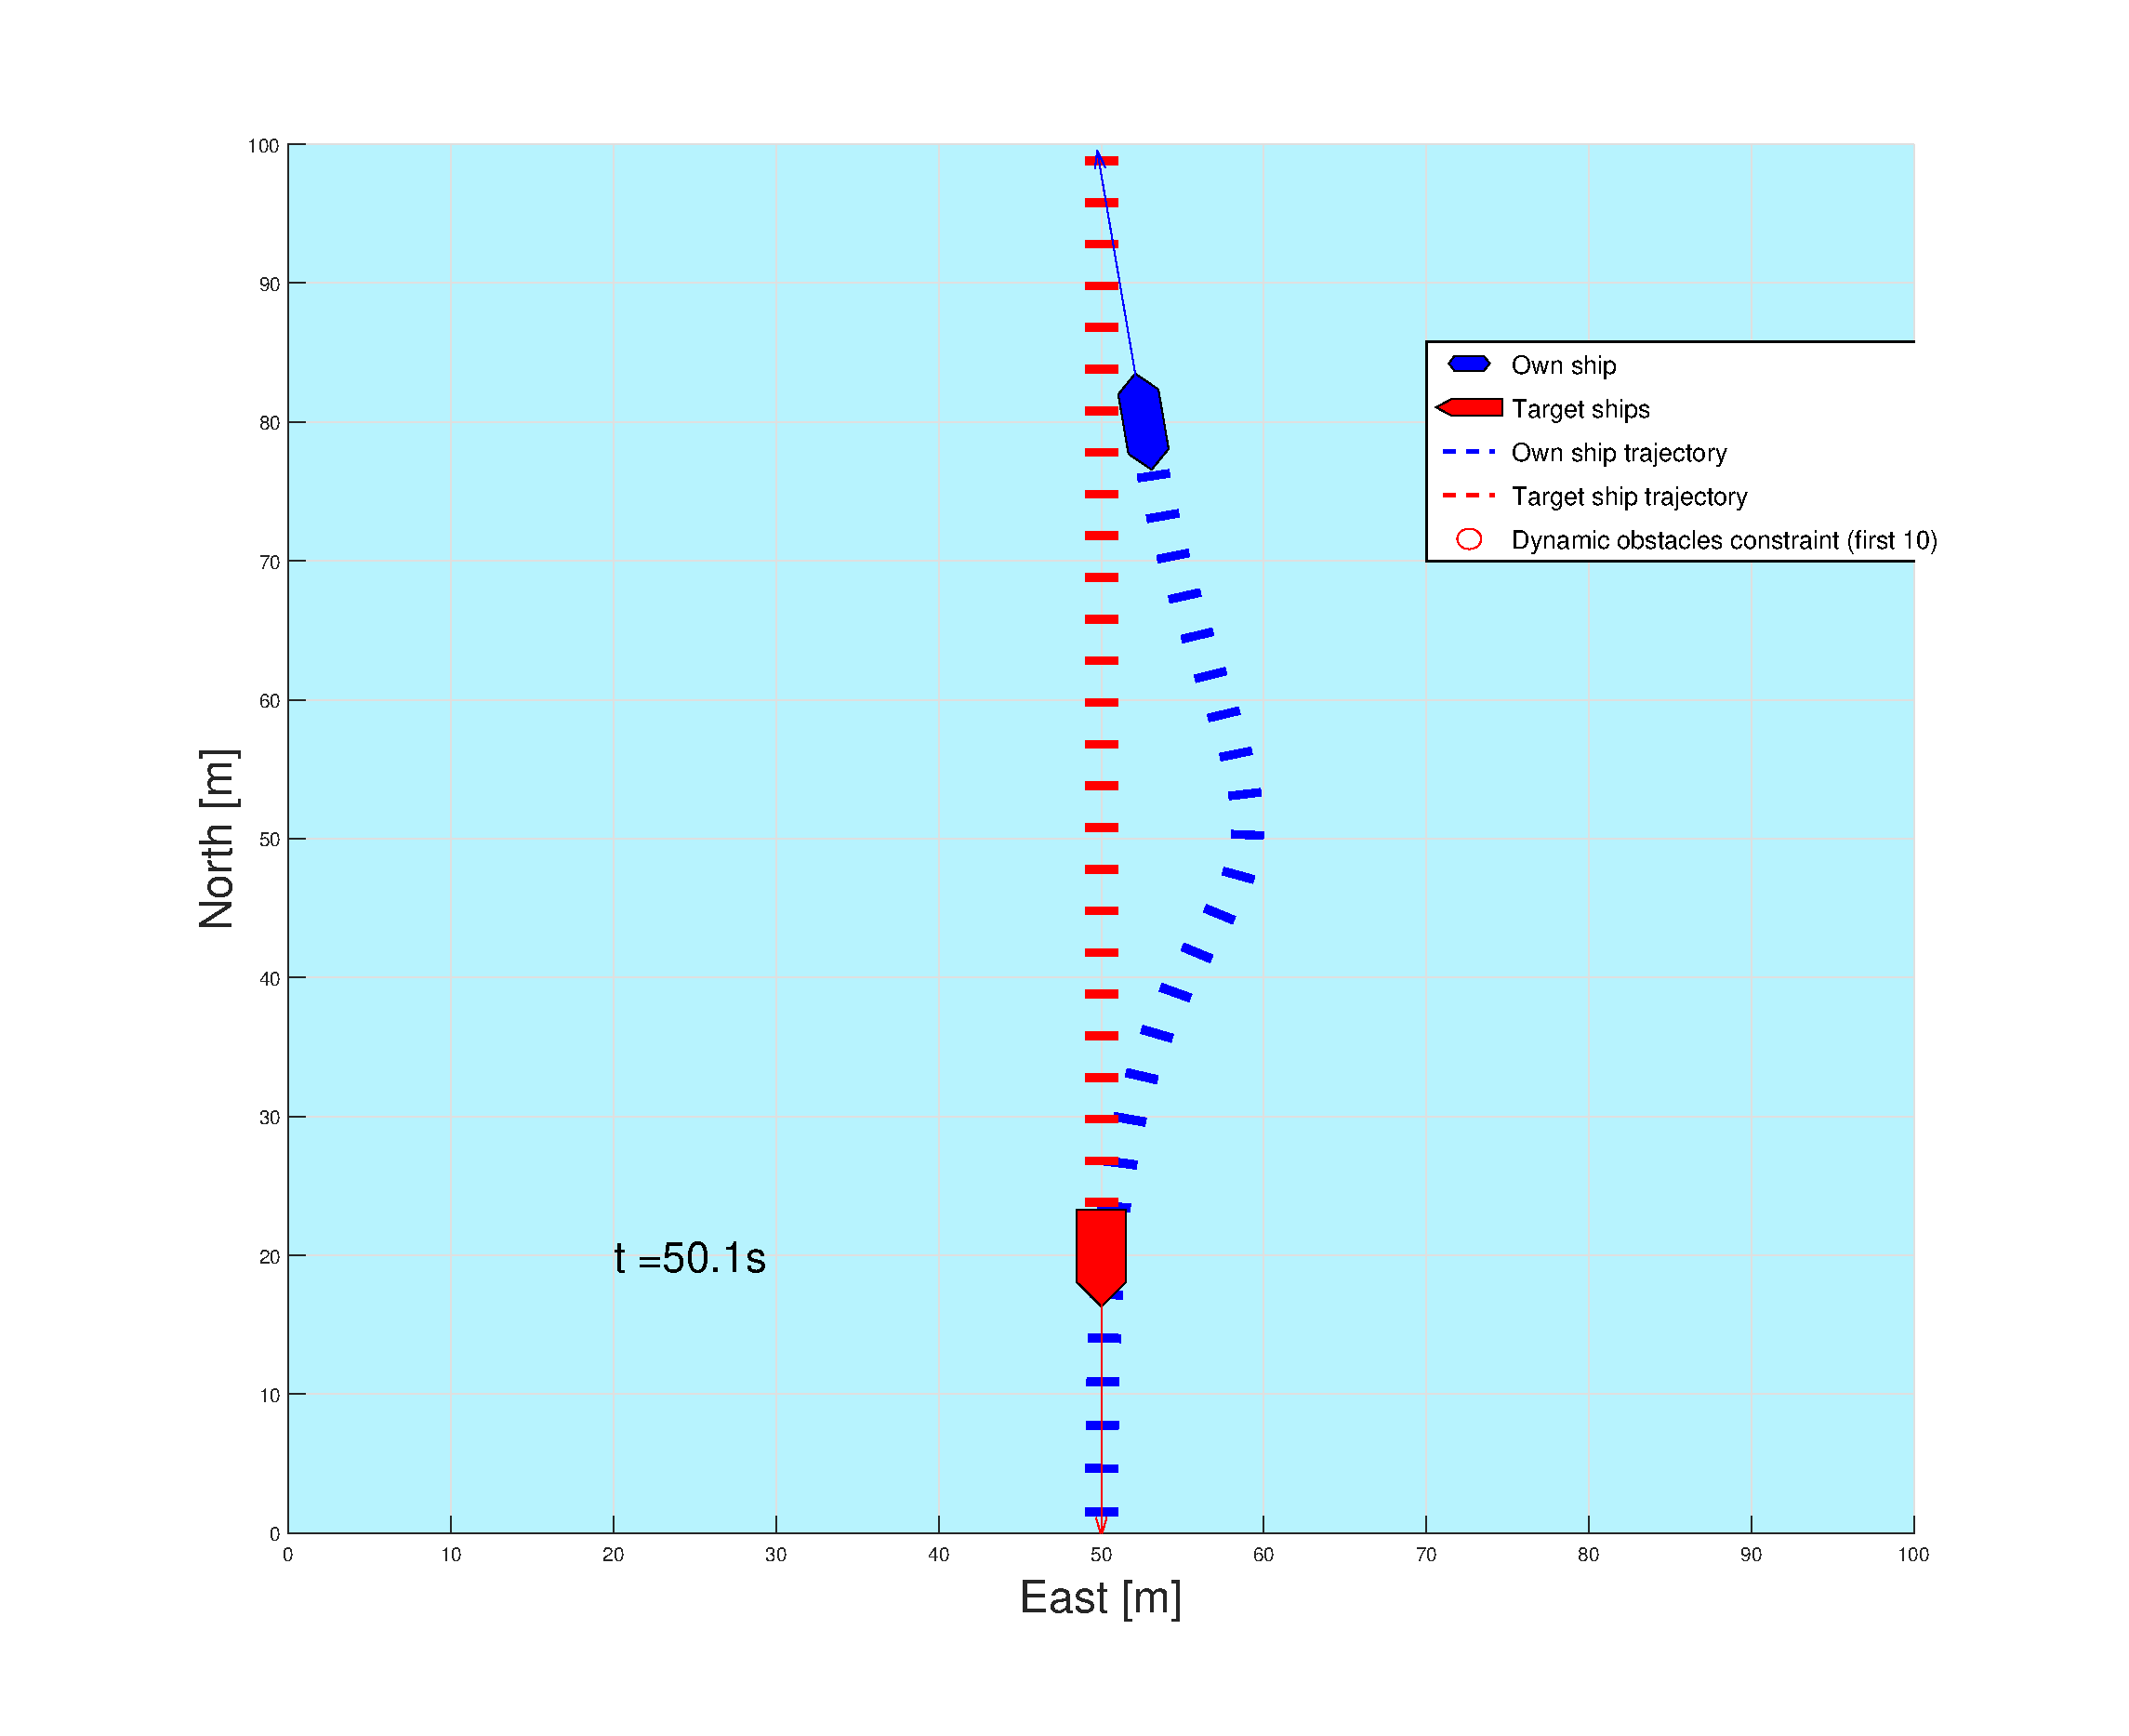
\includegraphics[width=\textwidth]{Images/Figures/enkel_HO/_Simple_0fig1_time=50}
%         \subcaption{}
%     \end{subfigure}
%     \hfill
%     \begin{subfigure}[b]{0.499\textwidth}
%         \centering
%         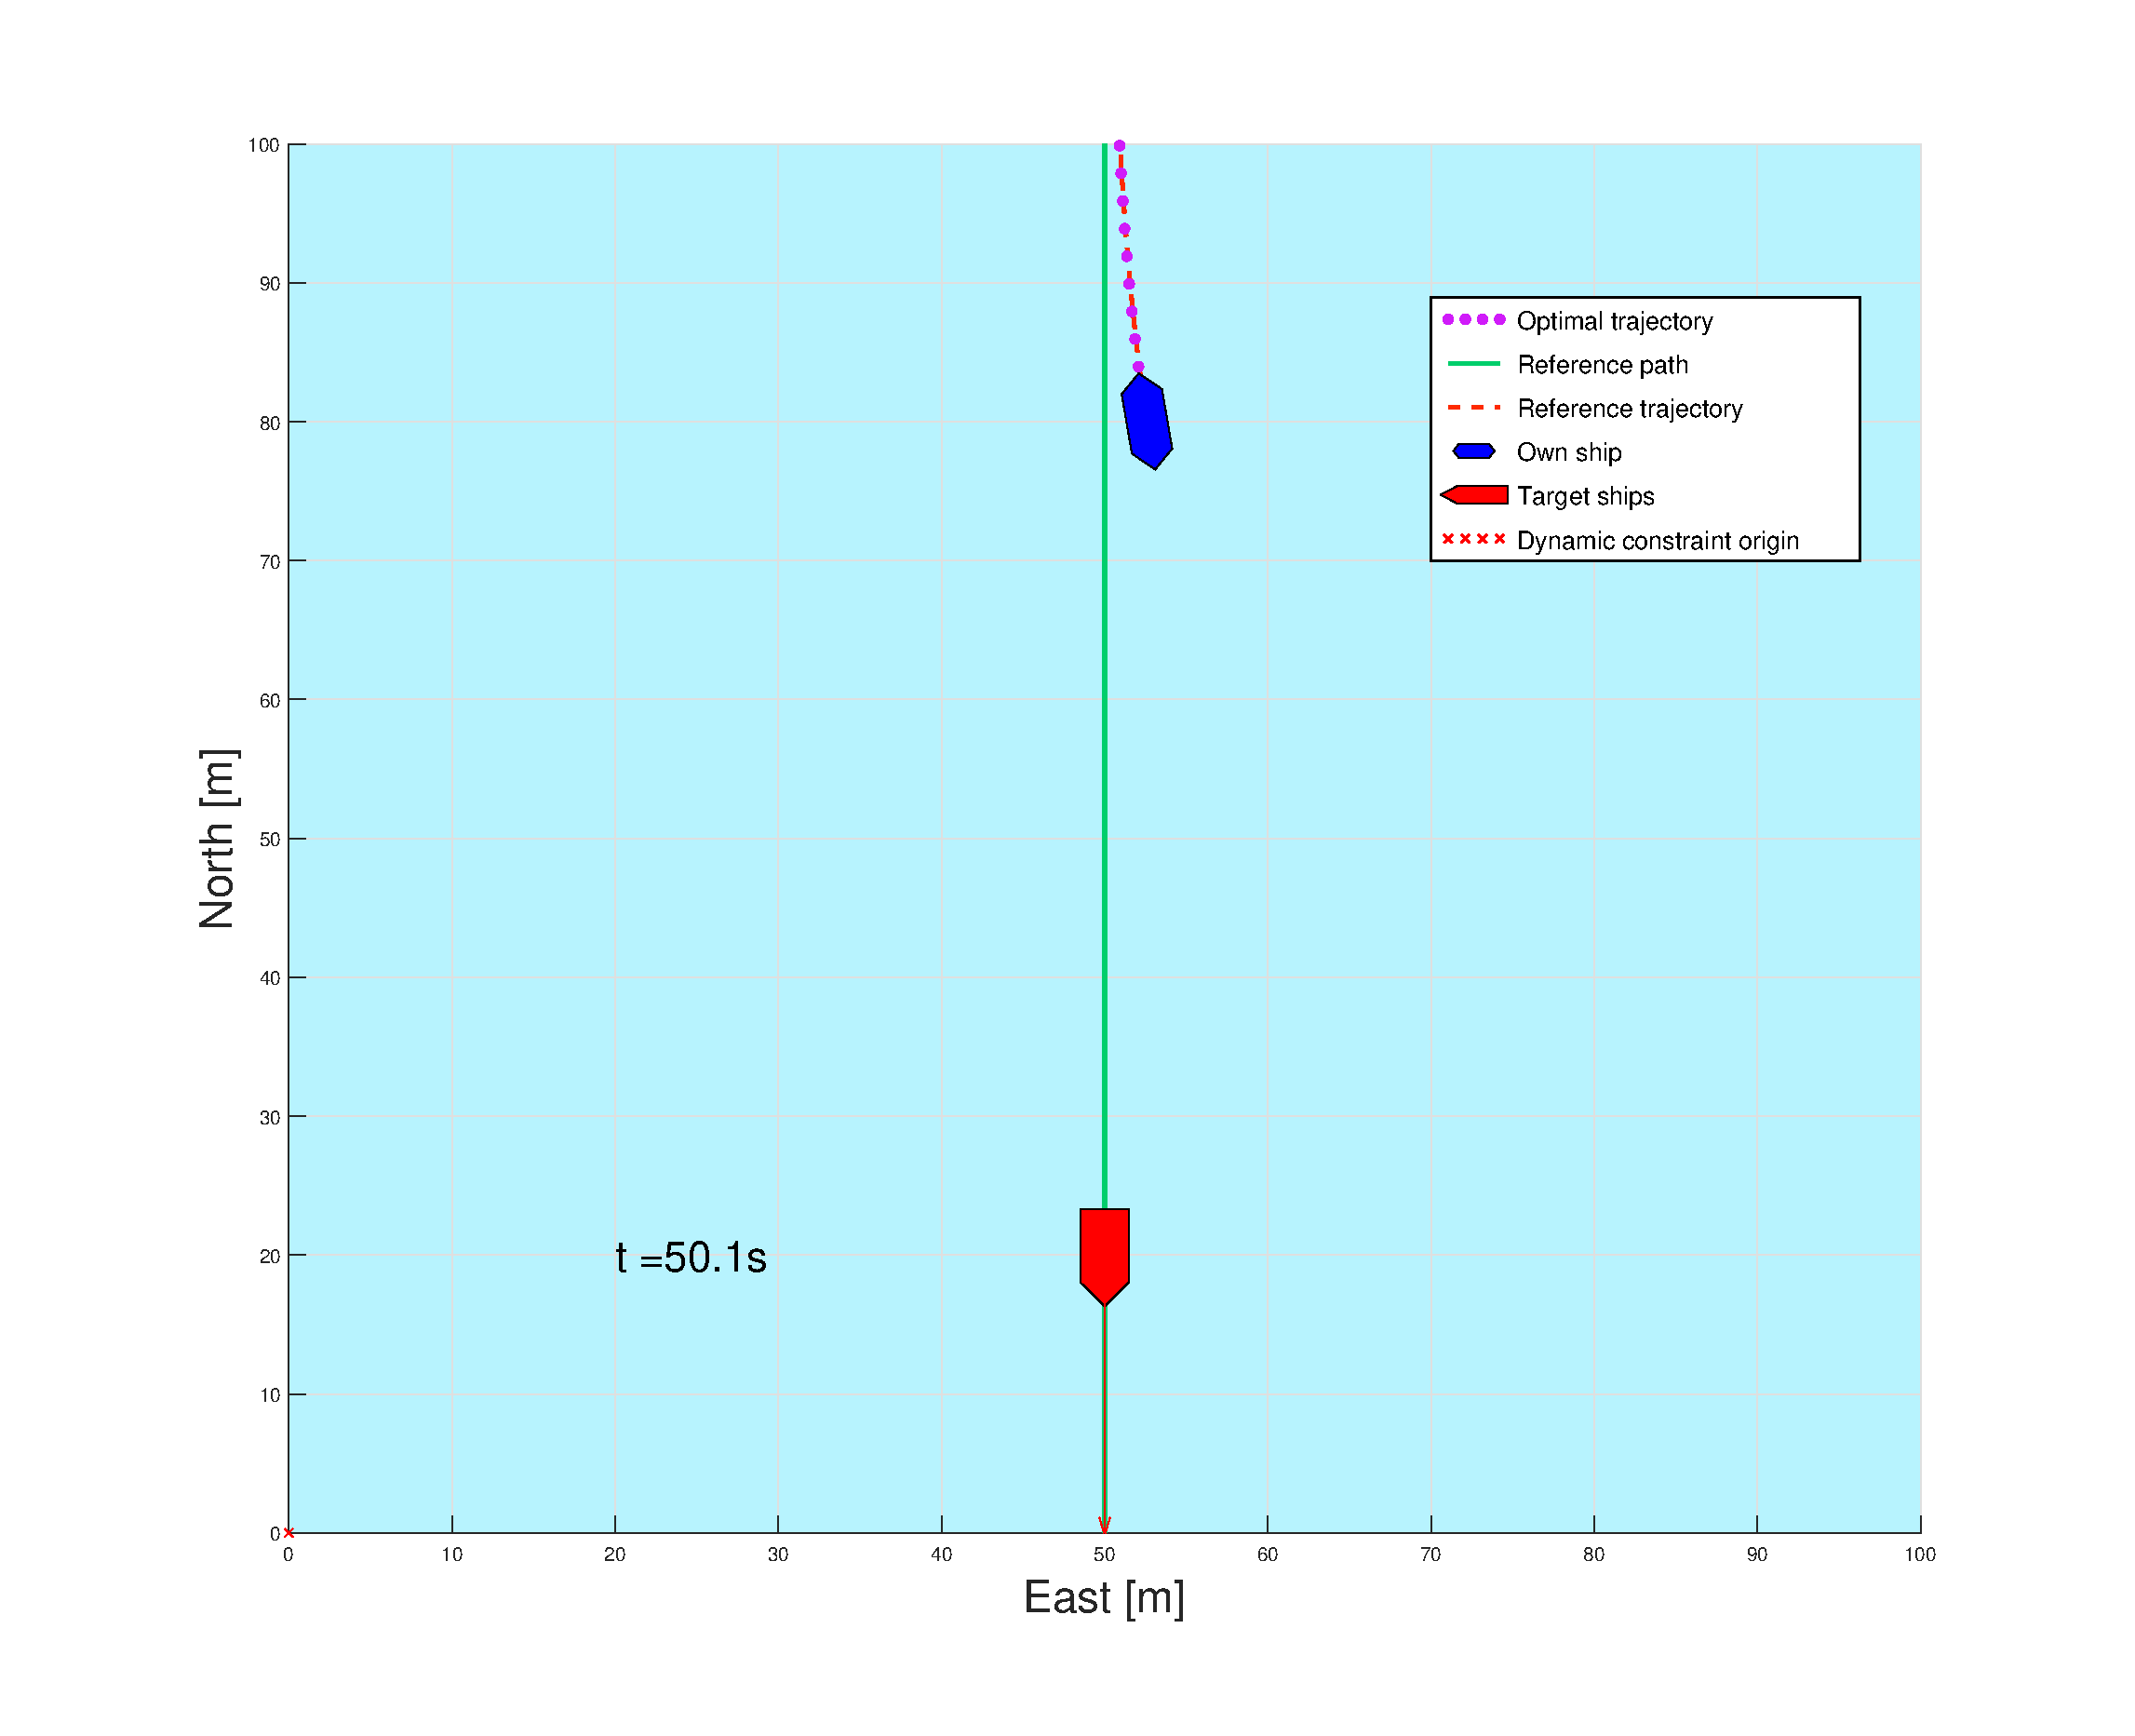
\includegraphics[width=\textwidth]{Images/Figures/enkel_HO/_Simple_0fig999_time=50}
%         \subcaption{}
%     \end{subfigure}
%     \hfill
%     \\
%     \begin{subfigure}[b]{0.49\textwidth}
%         \centering
%         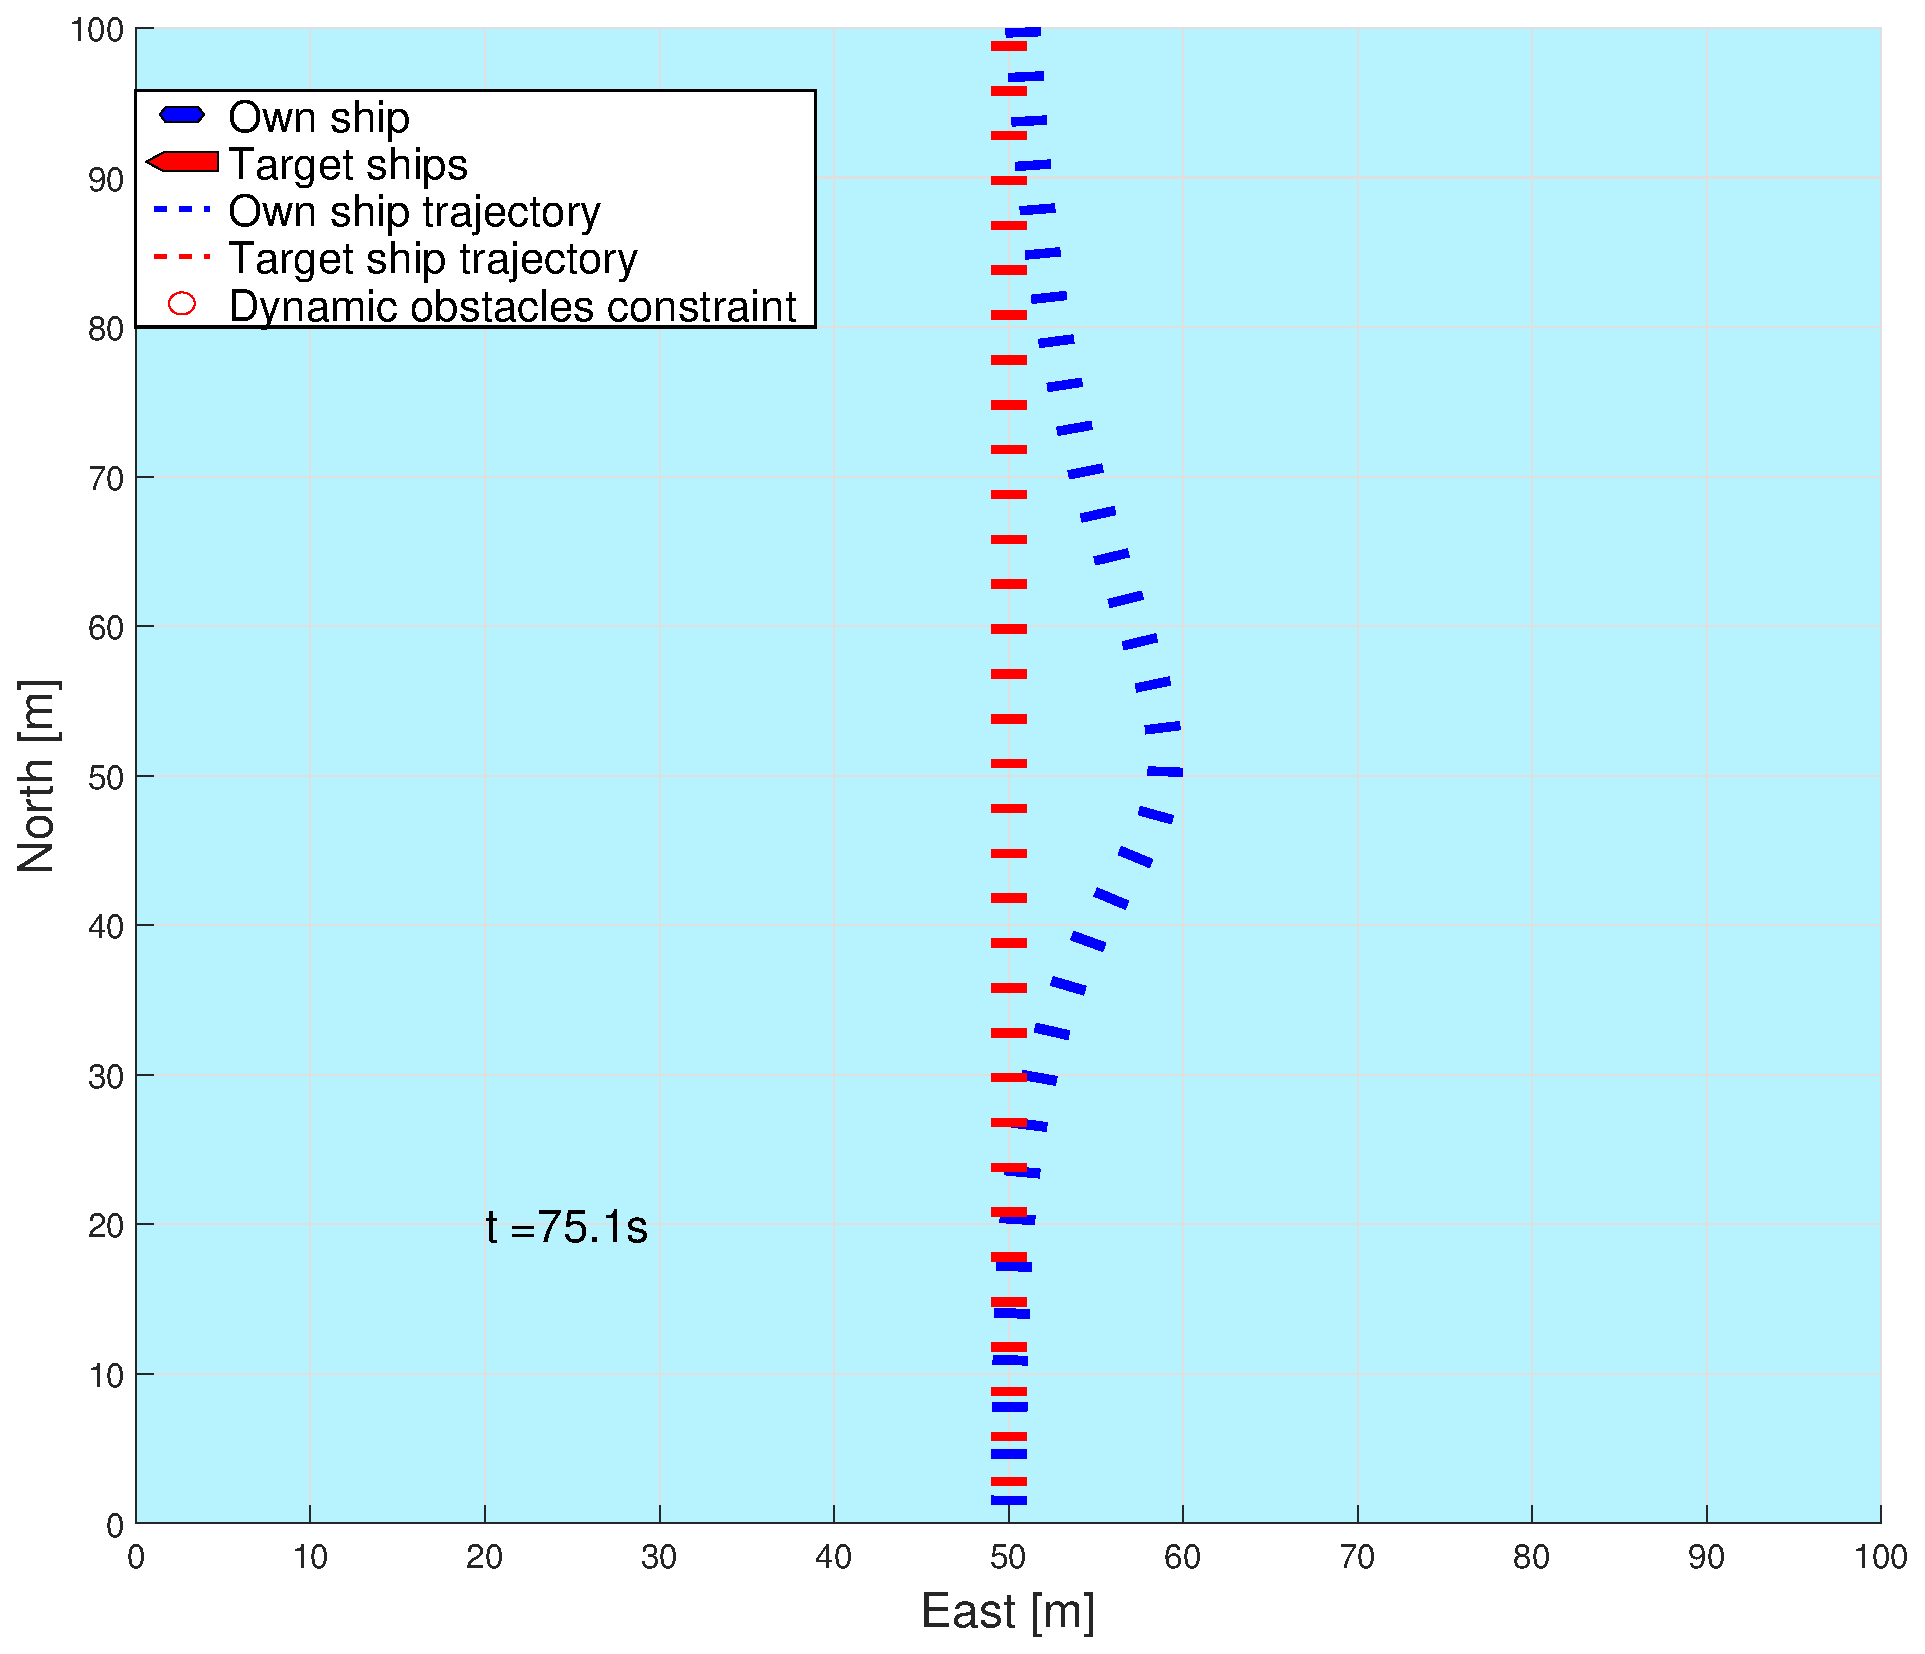
\includegraphics[width=\textwidth]{Images/Figures/enkel_HO/_Simple_0fig1_time=75}
%         \subcaption{}
%     \end{subfigure}
%     \hfill
%     \begin{subfigure}[b]{0.499\textwidth}
%         \centering
%         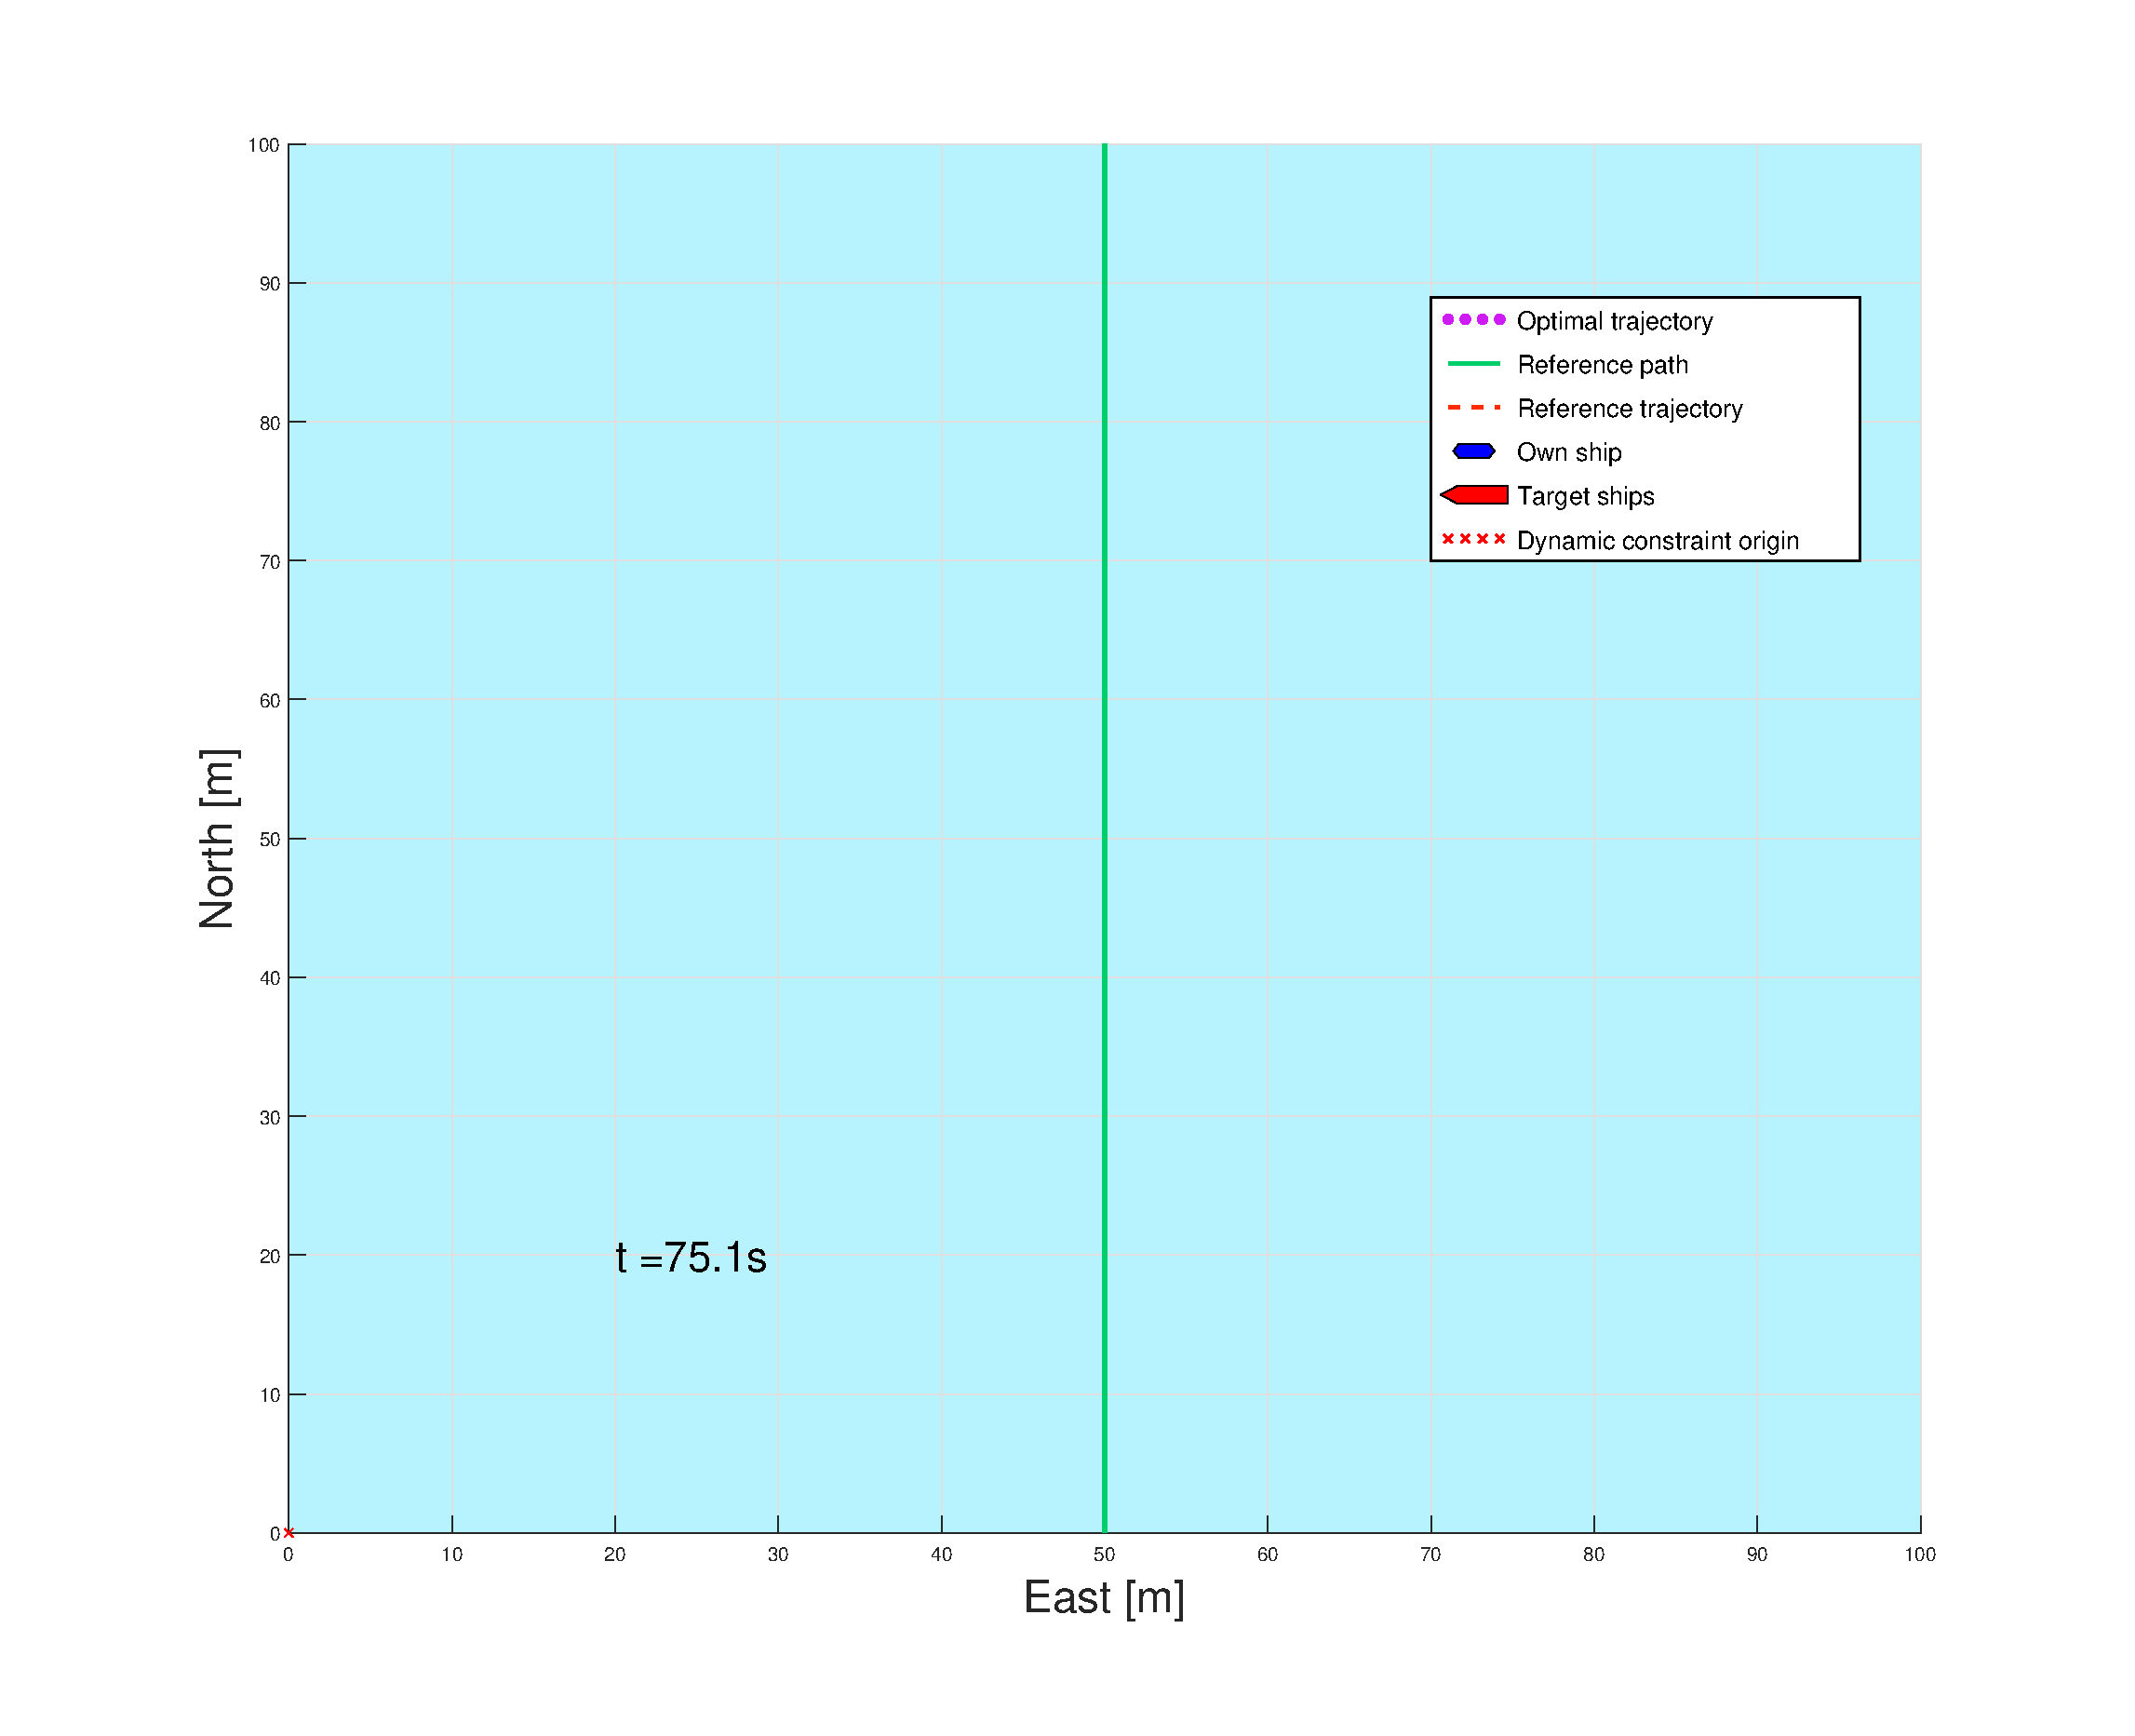
\includegraphics[width=\textwidth]{Images/Figures/enkel_HO/_Simple_0fig999_time=75}
%         \subcaption{}
%     \end{subfigure}
%     \hfill
%     \caption{Simple Head on With Prediction}
% \end{figure}

% \begin{figure}[!b] 
%     \begin{subfigure}[b]{0.49\textwidth}
%         \centering
%         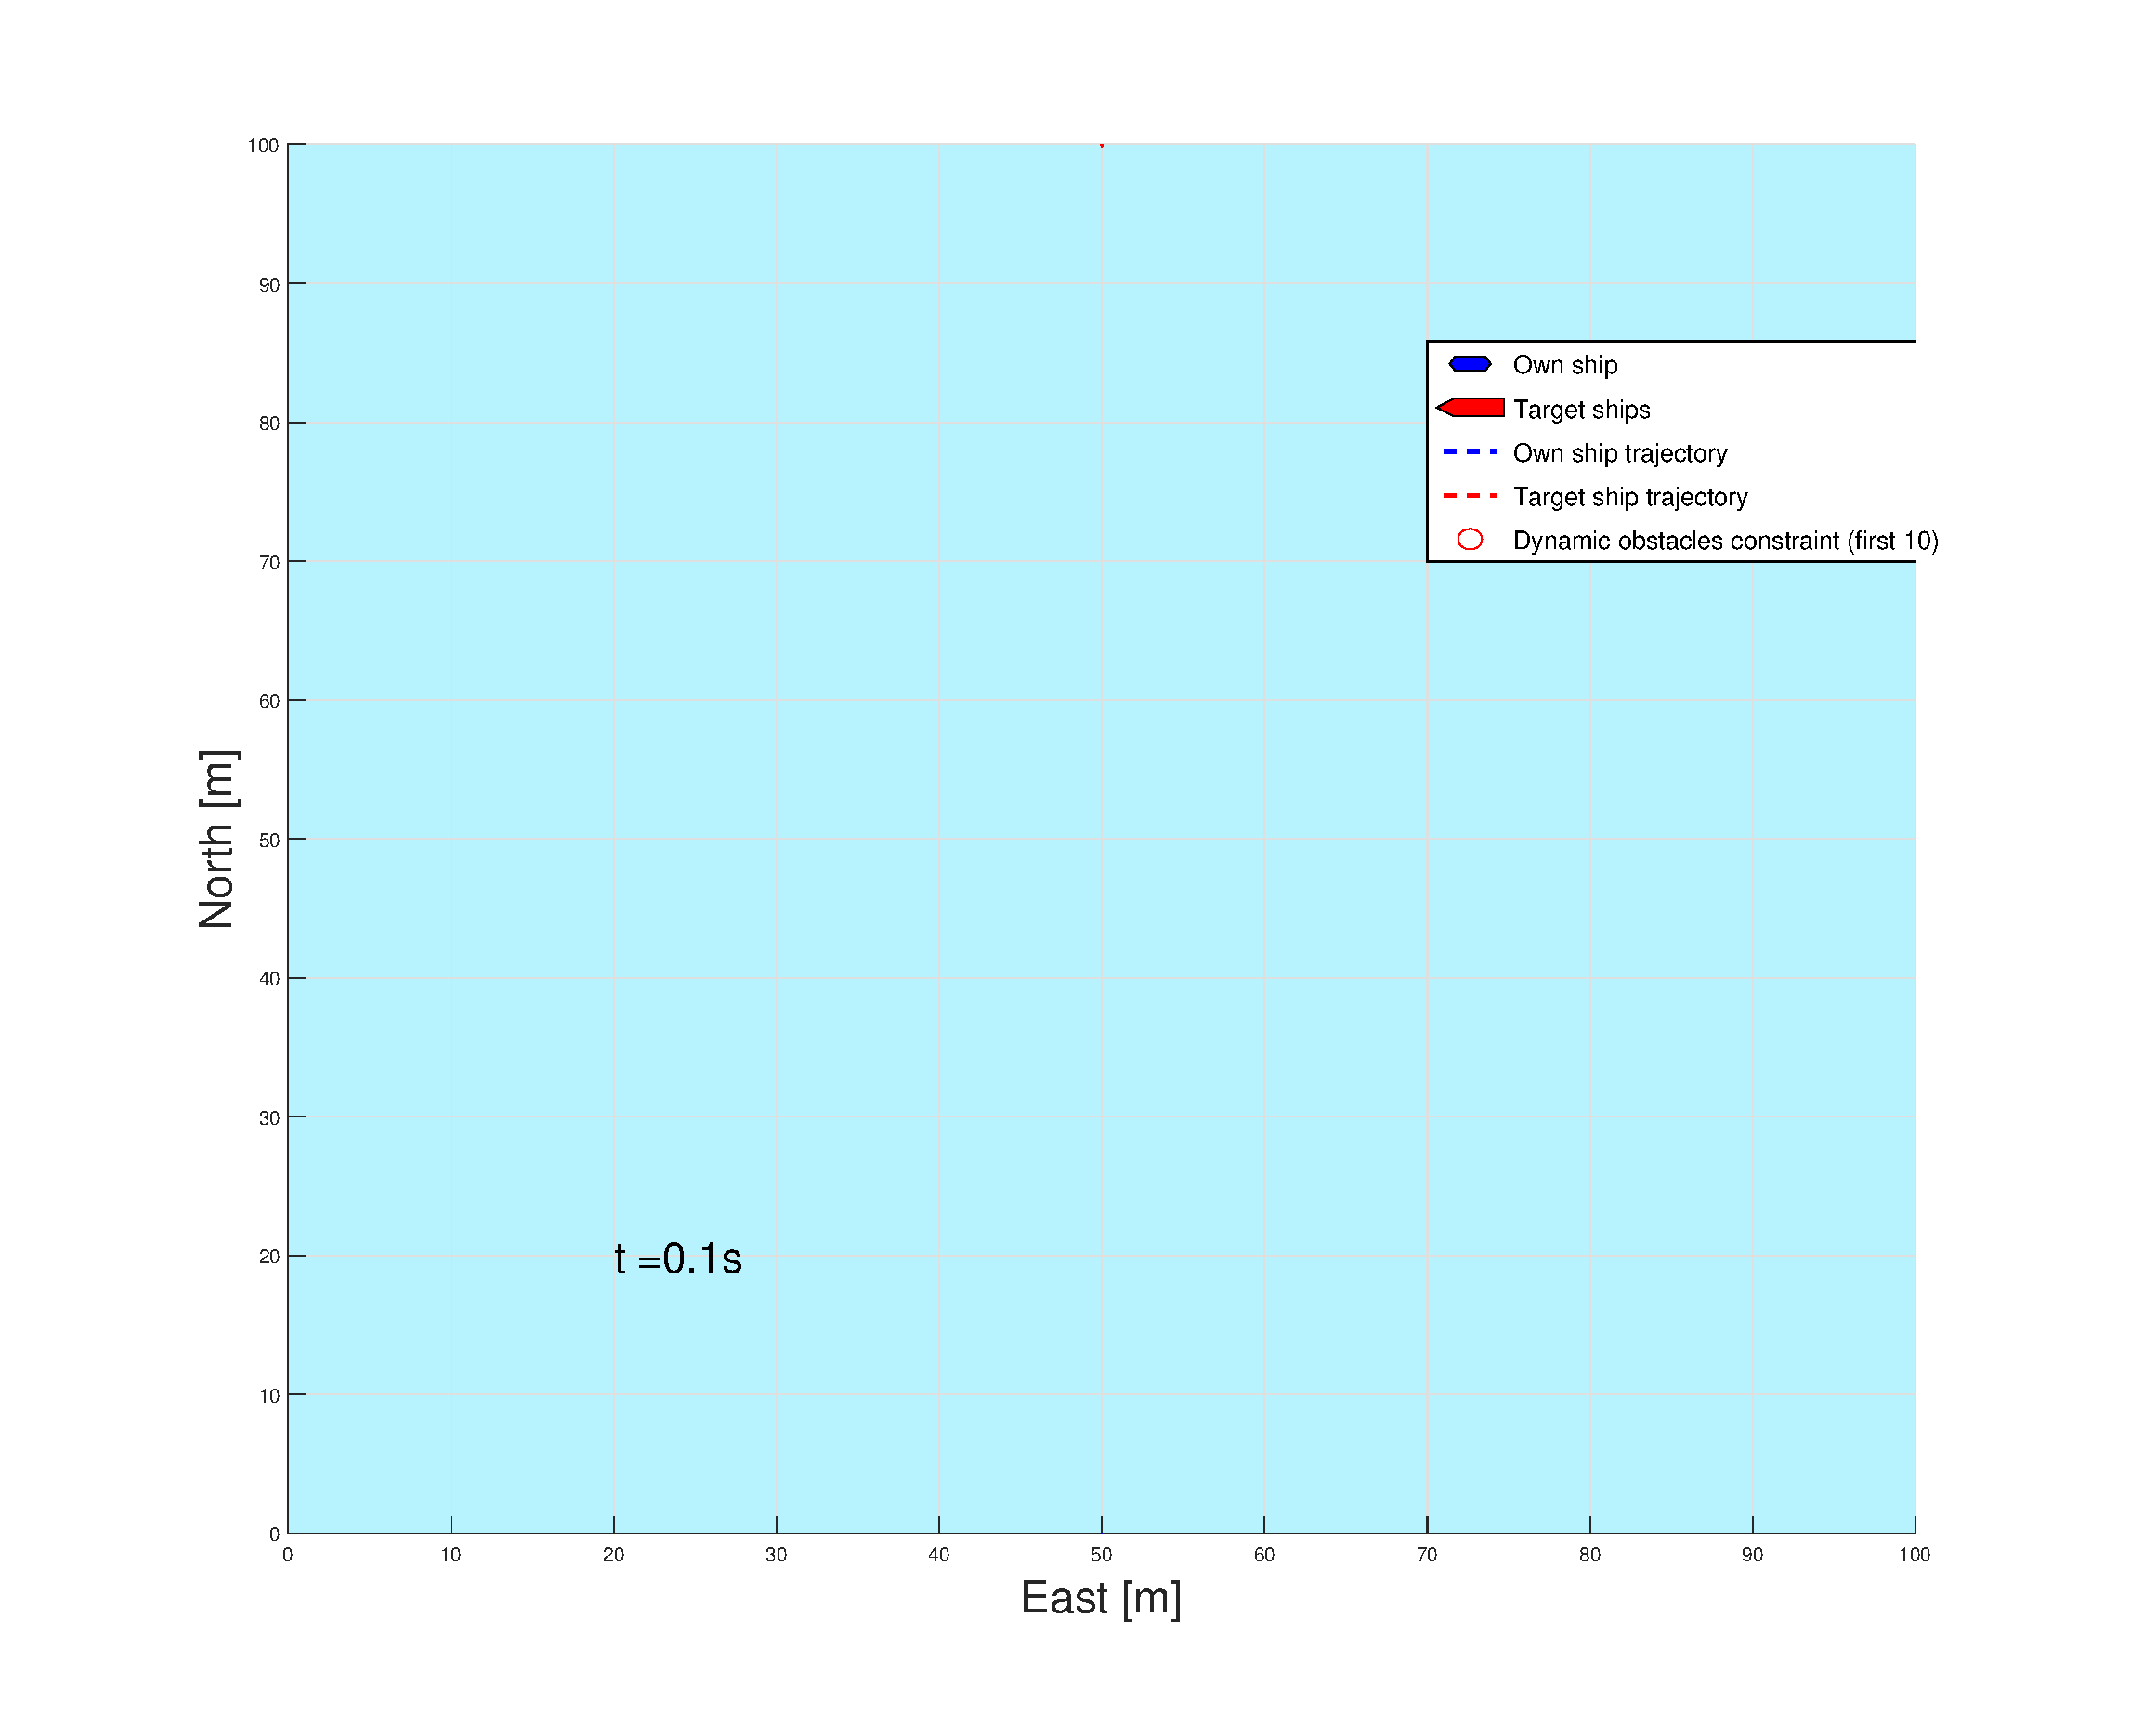
\includegraphics[width=\textwidth]{Images/Figures/enkel_HO/_Simple_1fig1_time=0}
%         \subcaption{}
%     \end{subfigure}
%     \hfill
%     \begin{subfigure}[b]{0.499\textwidth}
%         \centering
%         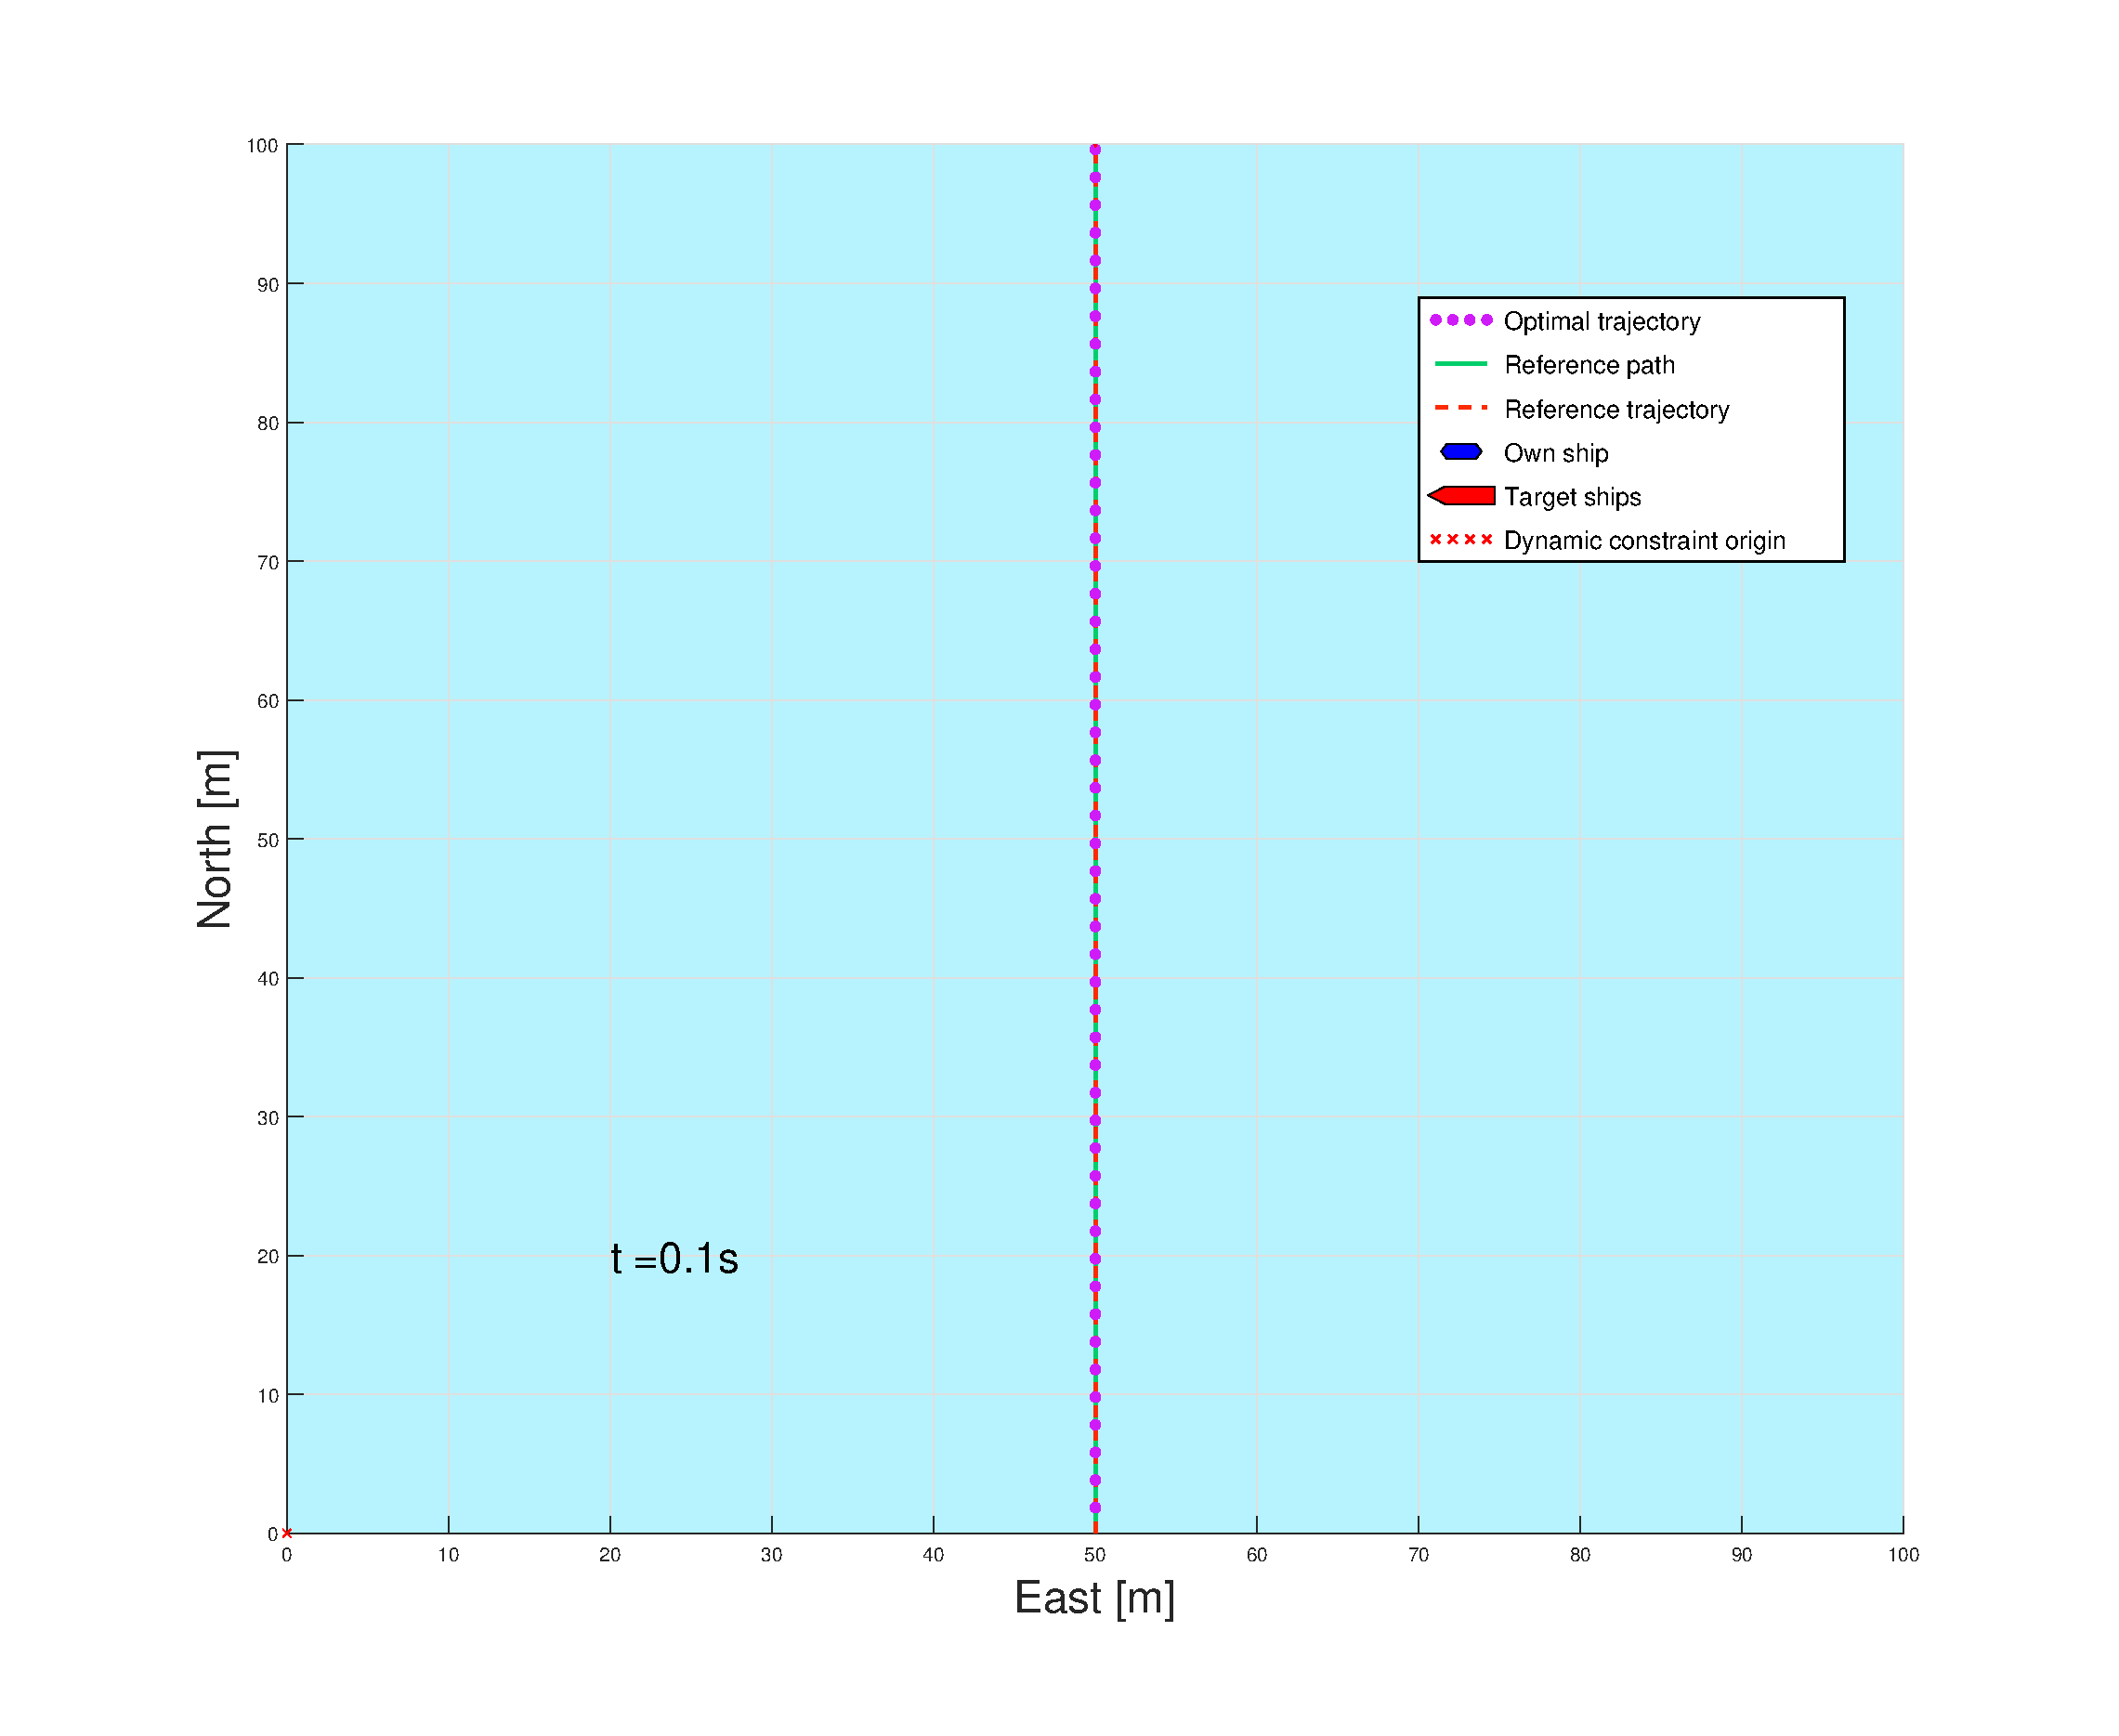
\includegraphics[width=\textwidth]{Images/Figures/enkel_HO/_Simple_1fig999_time=0}
%         \subcaption{}
%     \end{subfigure}
%     \hfill
%     \\
%     \begin{subfigure}[b]{0.49\textwidth}
%         \centering
%         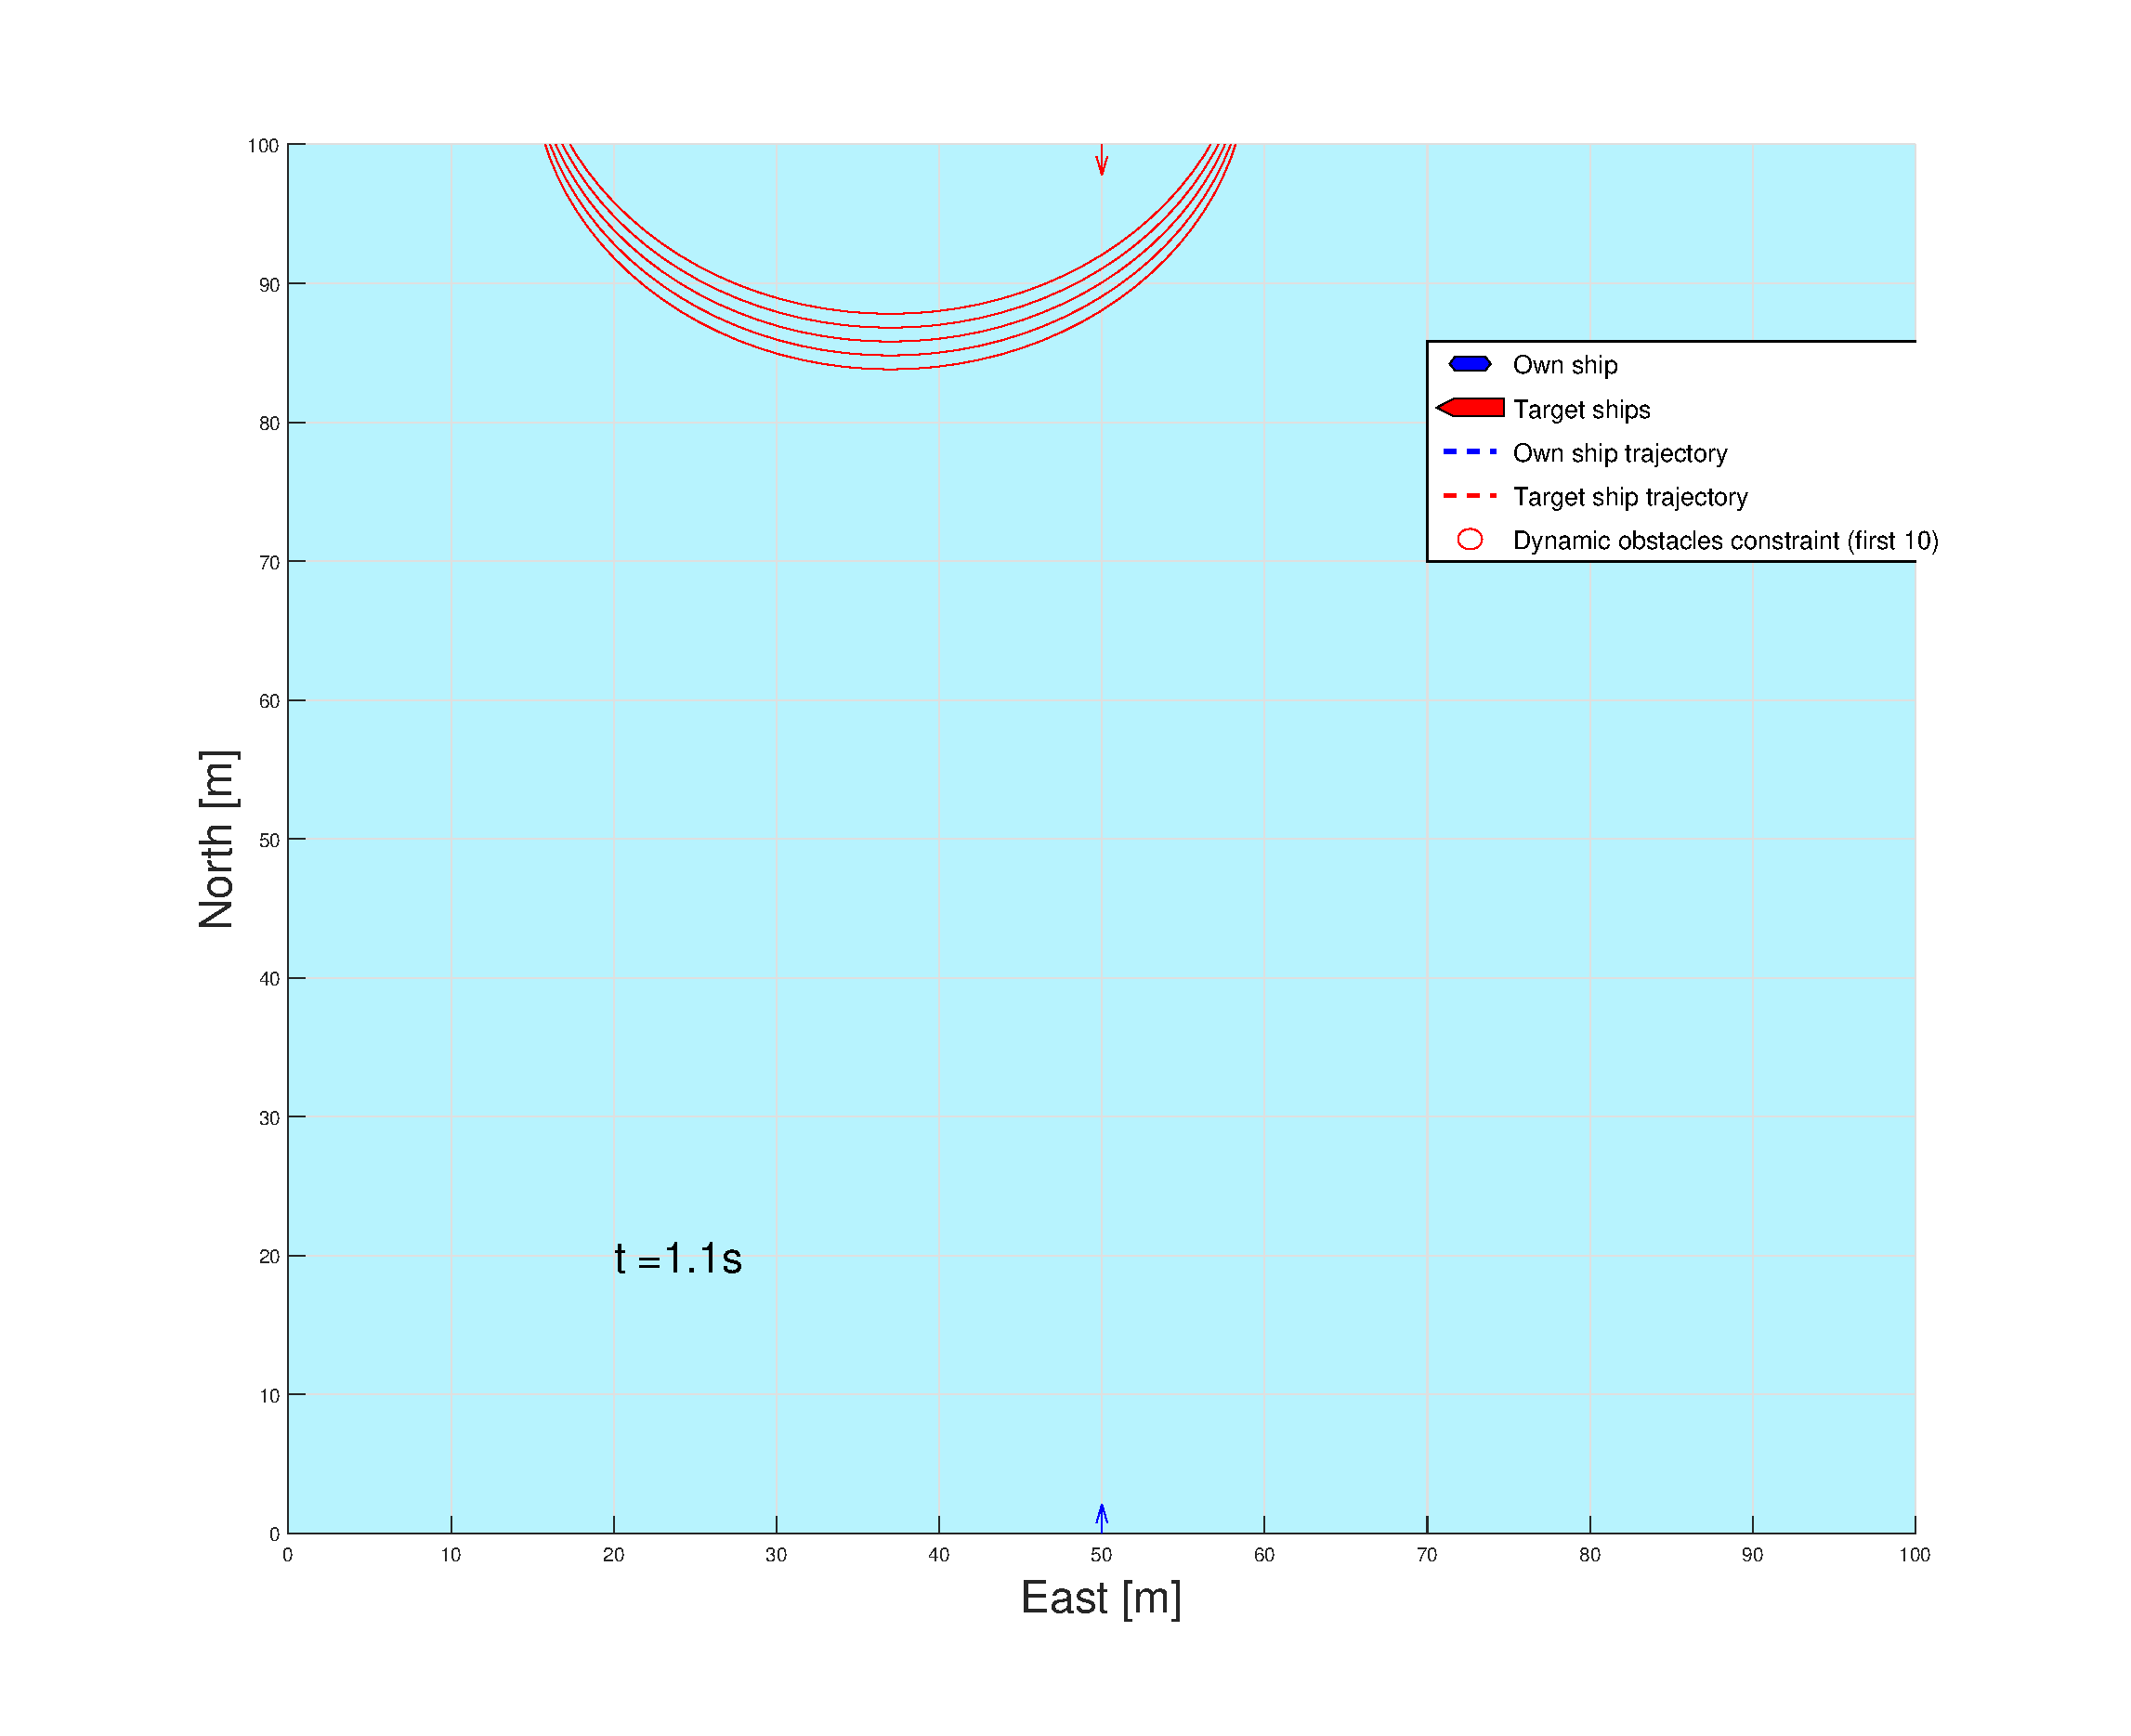
\includegraphics[width=\textwidth]{Images/Figures/enkel_HO/_Simple_1fig1_time=1}
%         \subcaption{}
%     \end{subfigure}
%     \hfill
%     \begin{subfigure}[b]{0.499\textwidth}
%         \centering
%         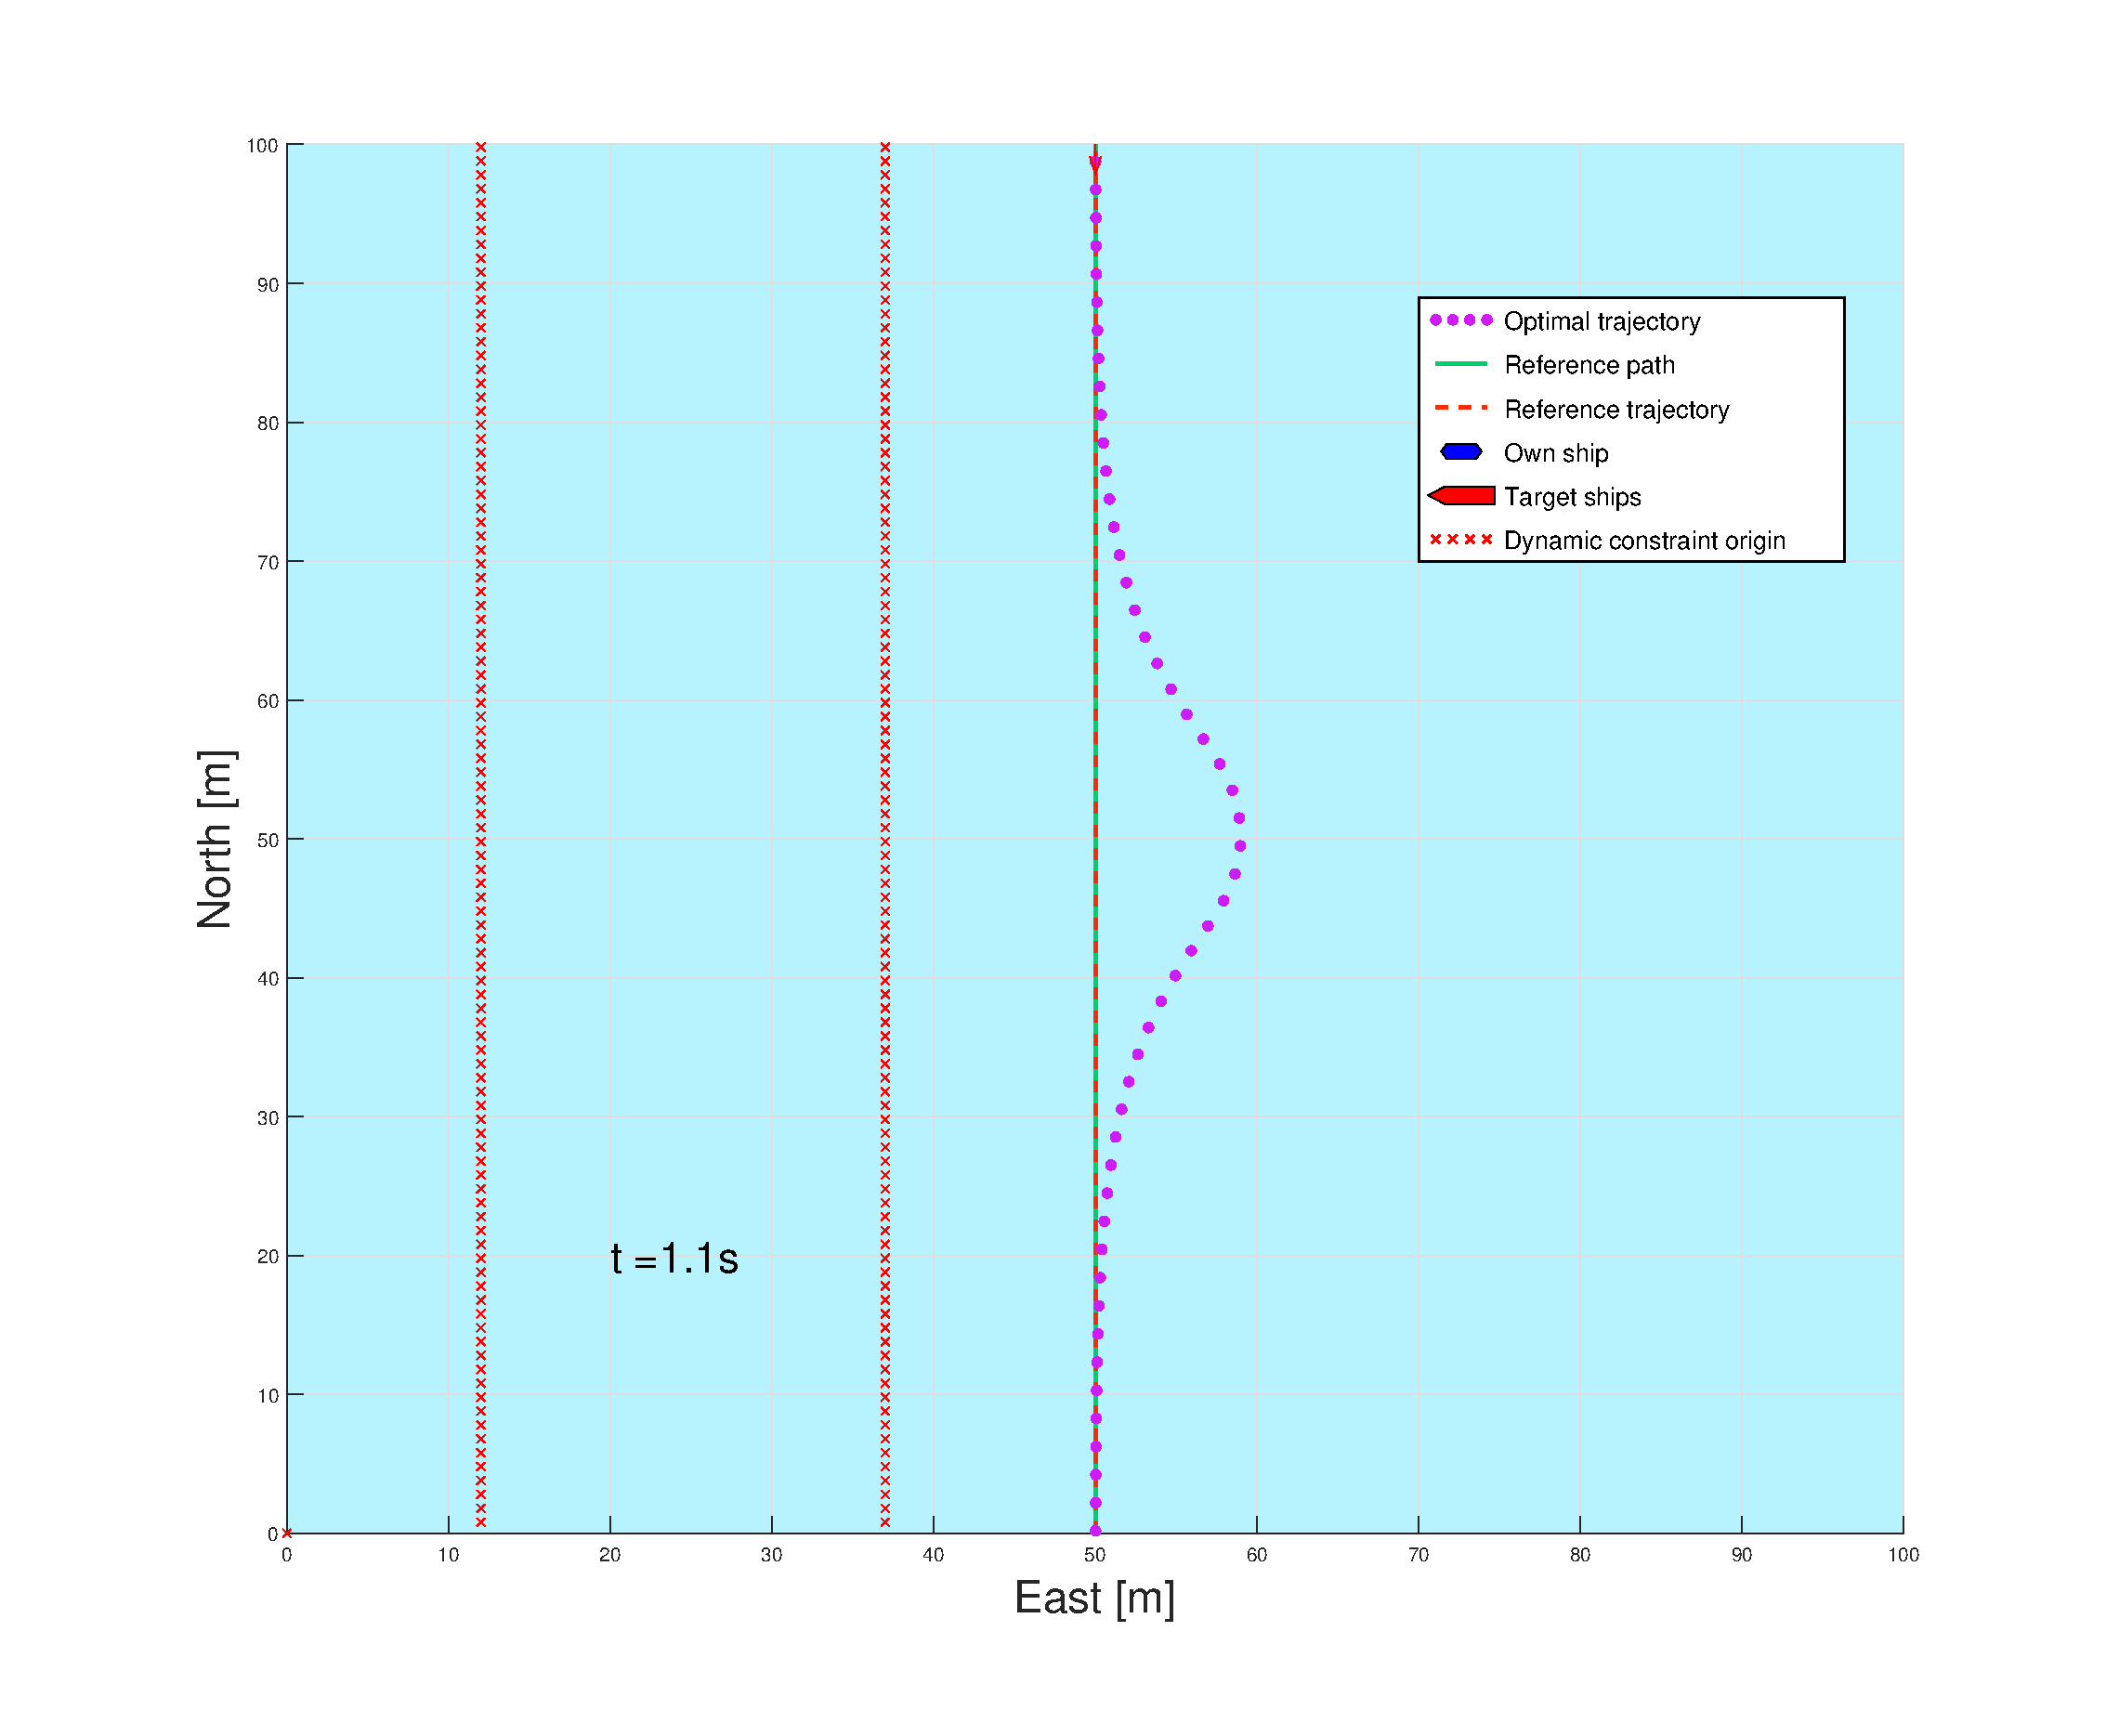
\includegraphics[width=\textwidth]{Images/Figures/enkel_HO/_Simple_1fig999_time=1}
%         \subcaption{}
%     \end{subfigure}
%     \hfill
%     \\
%     \begin{subfigure}[b]{0.49\textwidth}
%         \centering
%         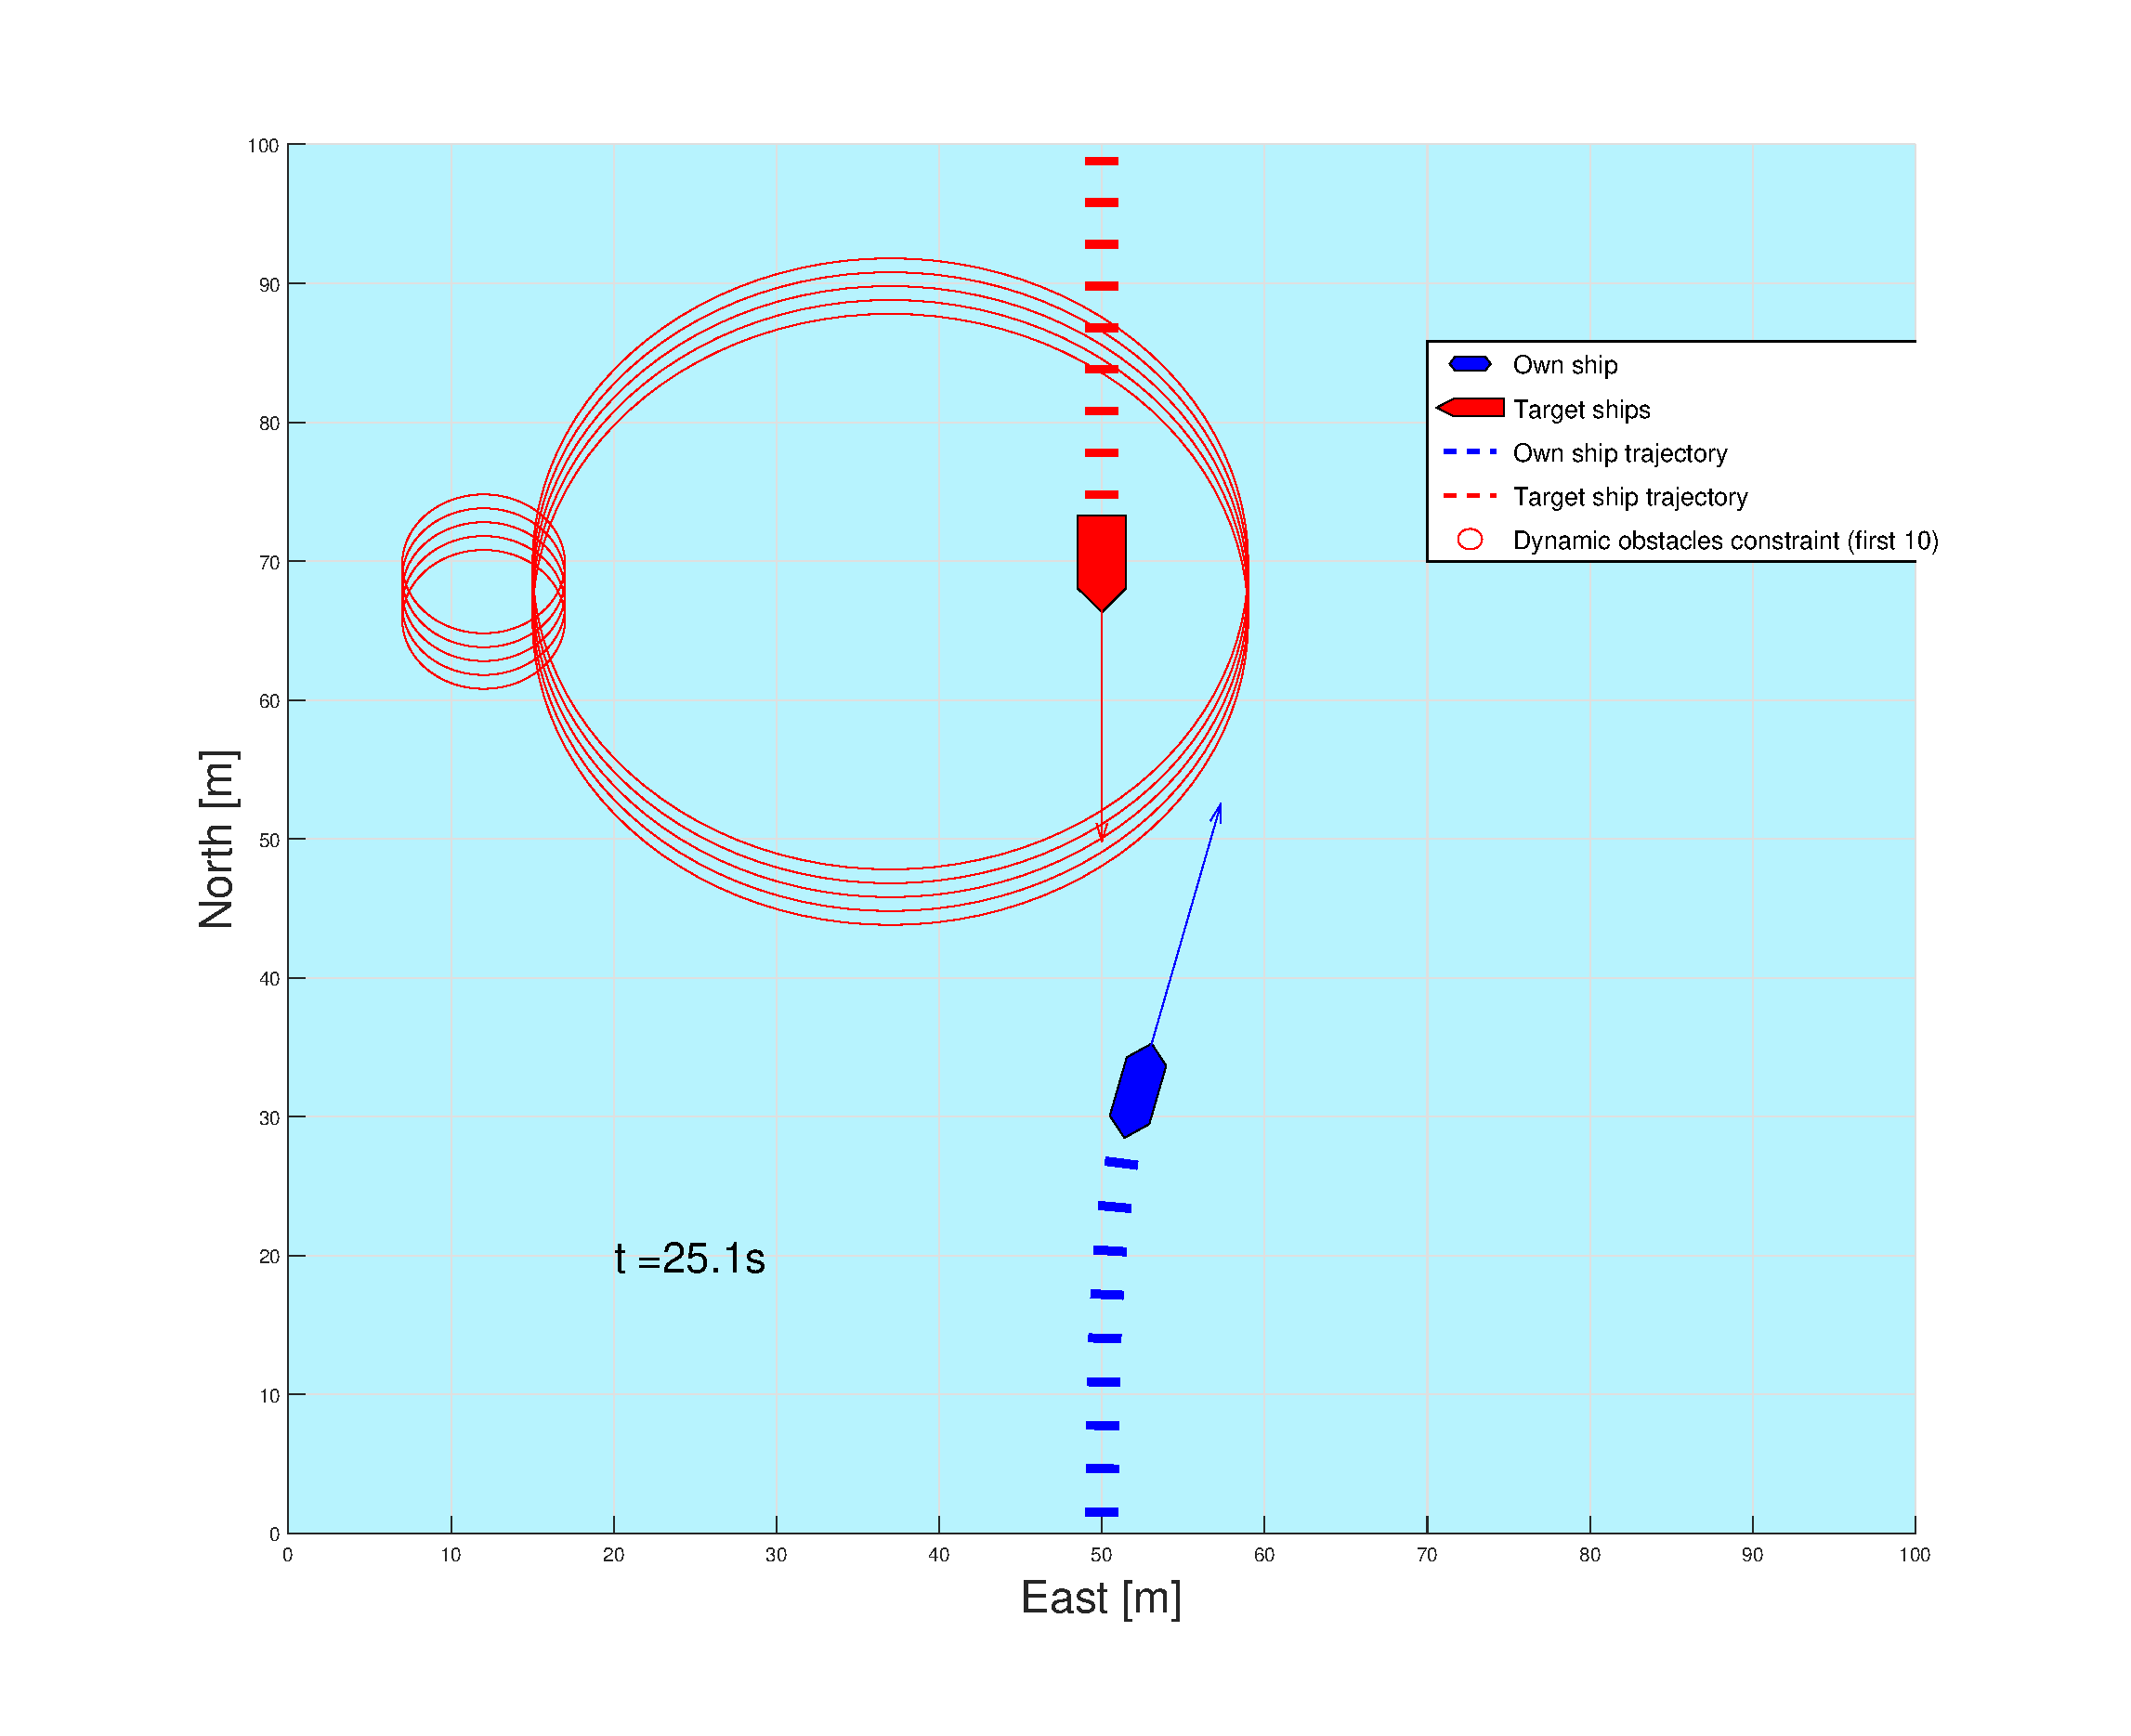
\includegraphics[width=\textwidth]{Images/Figures/enkel_HO/_Simple_1fig1_time=25}
%         \subcaption{}
%     \end{subfigure}
%     \hfill
%     \begin{subfigure}[b]{0.499\textwidth}
%         \centering
%         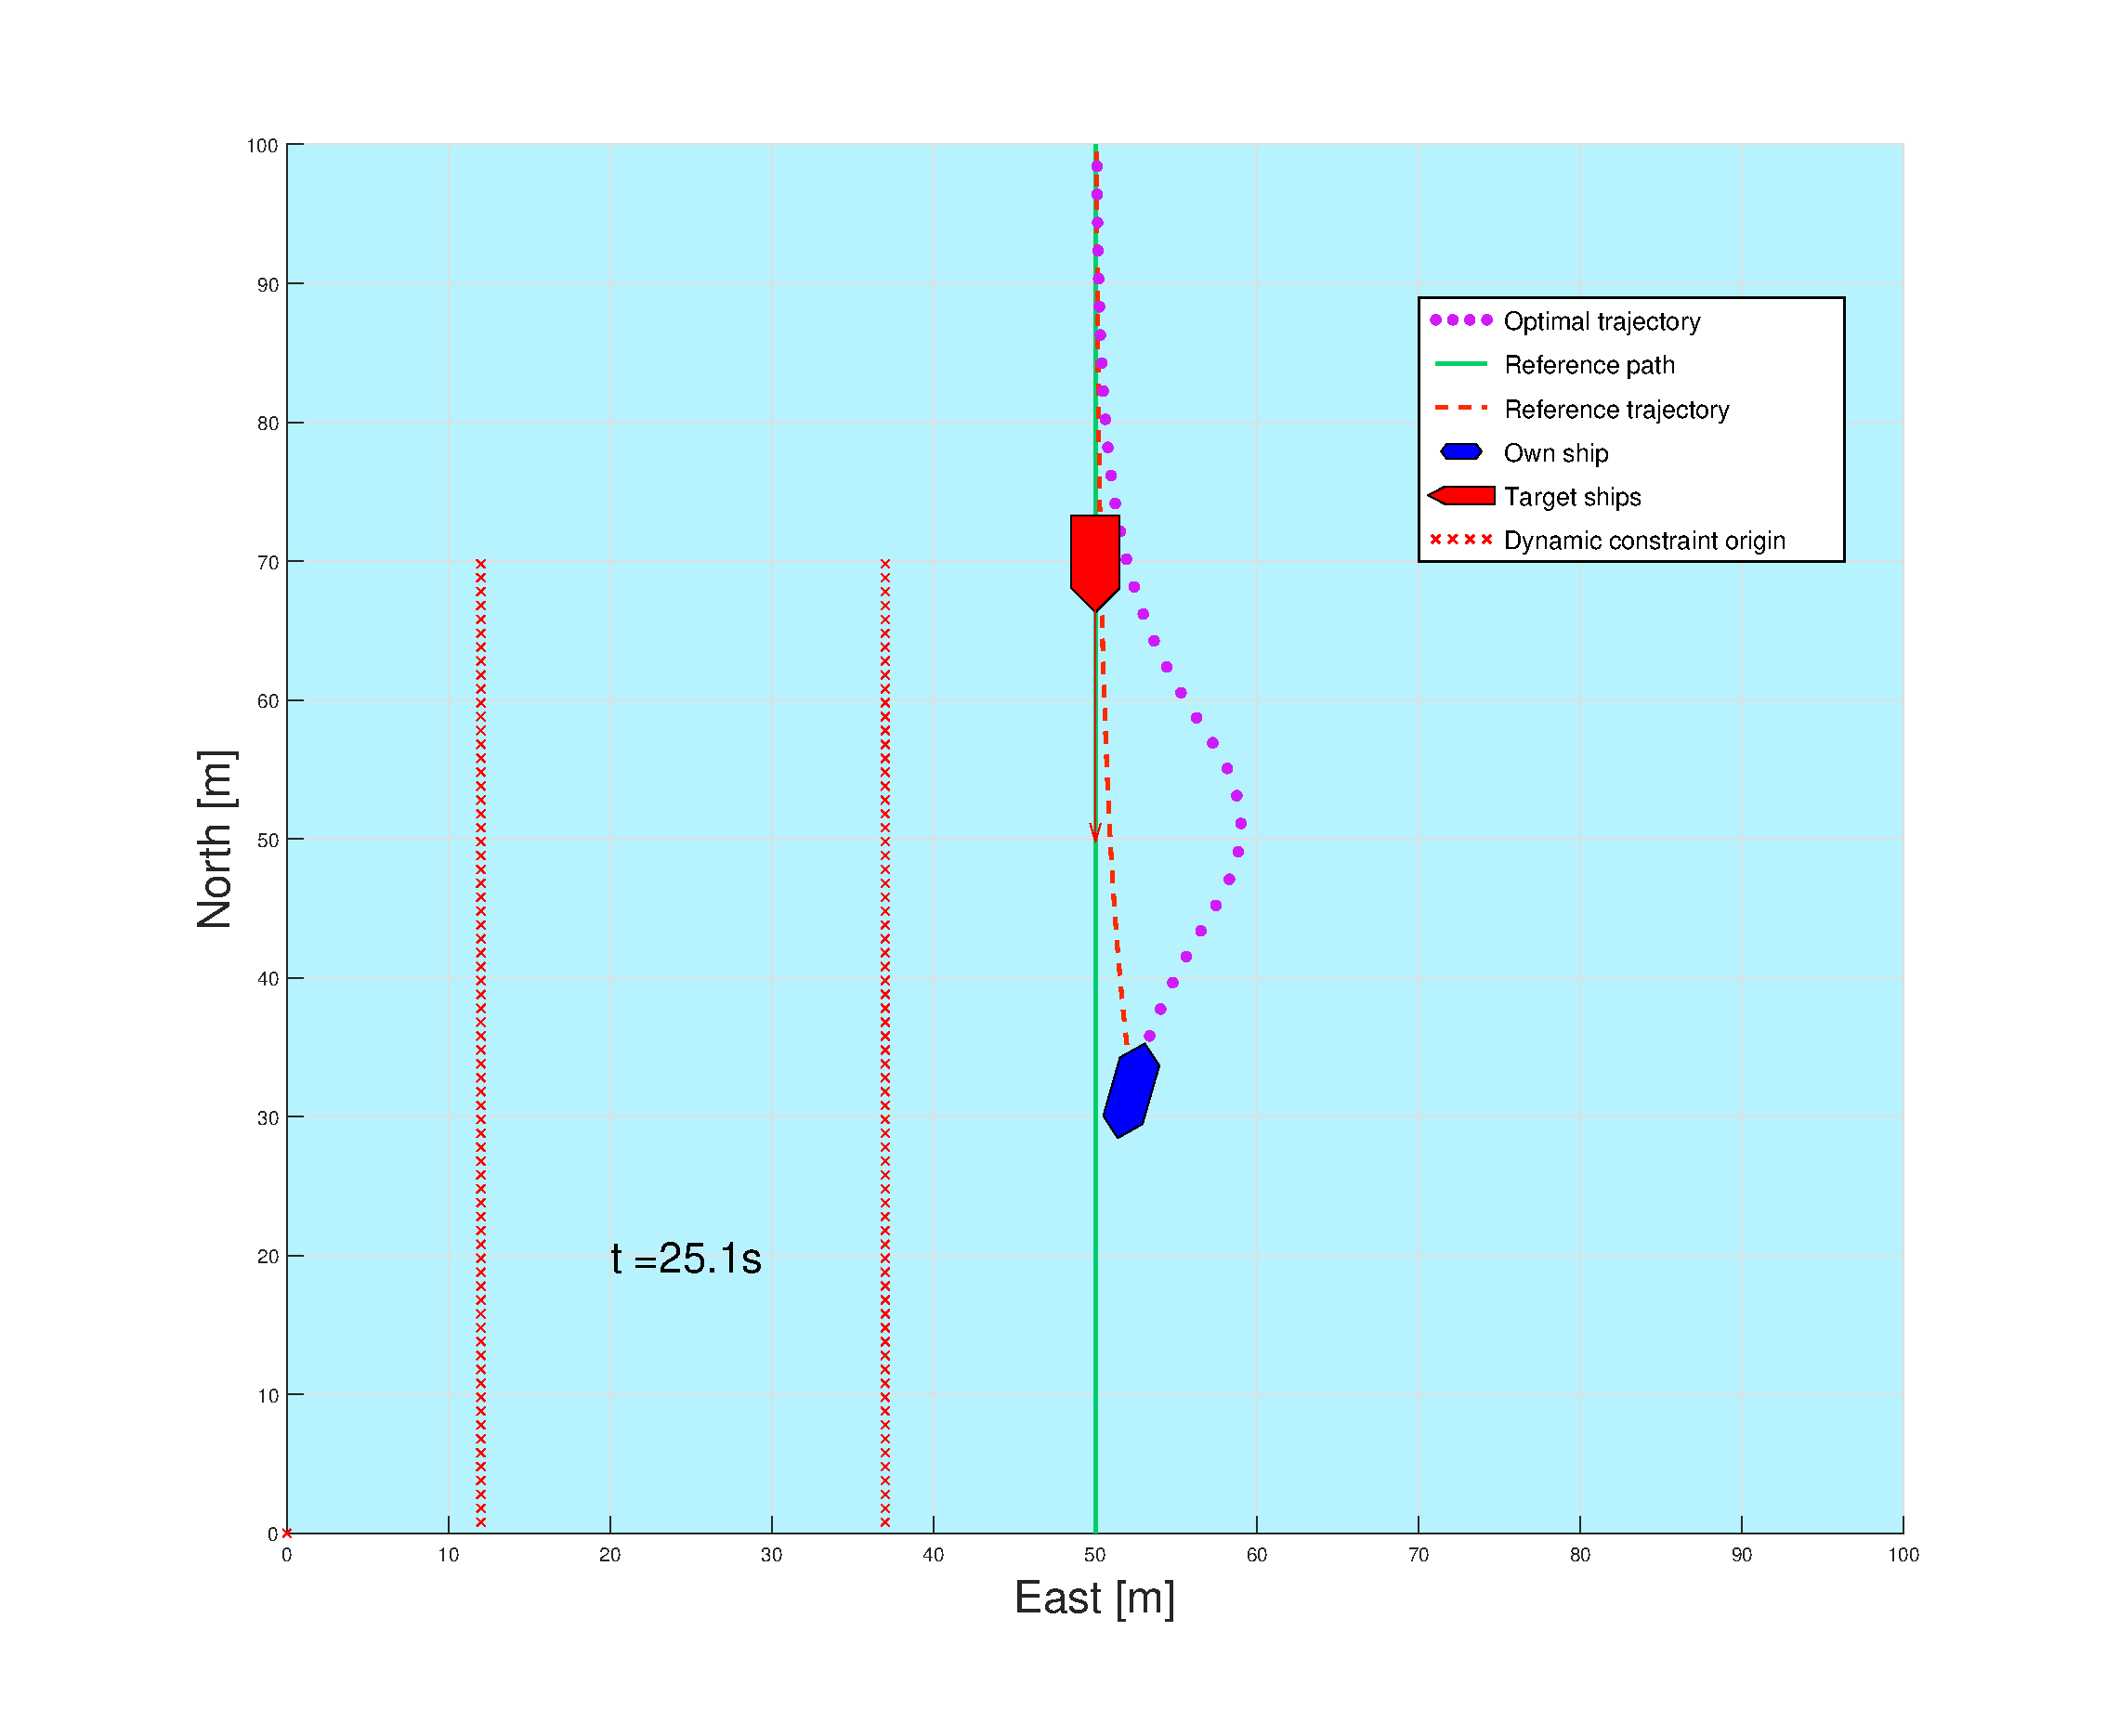
\includegraphics[width=\textwidth]{Images/Figures/enkel_HO/_Simple_1fig999_time=25}
%         \subcaption{}
%     \end{subfigure}
%     \hfill
% \end{figure}%
% \begin{figure}[ht]\ContinuedFloat
%     \begin{subfigure}[b]{0.49\textwidth}
%         \centering
%         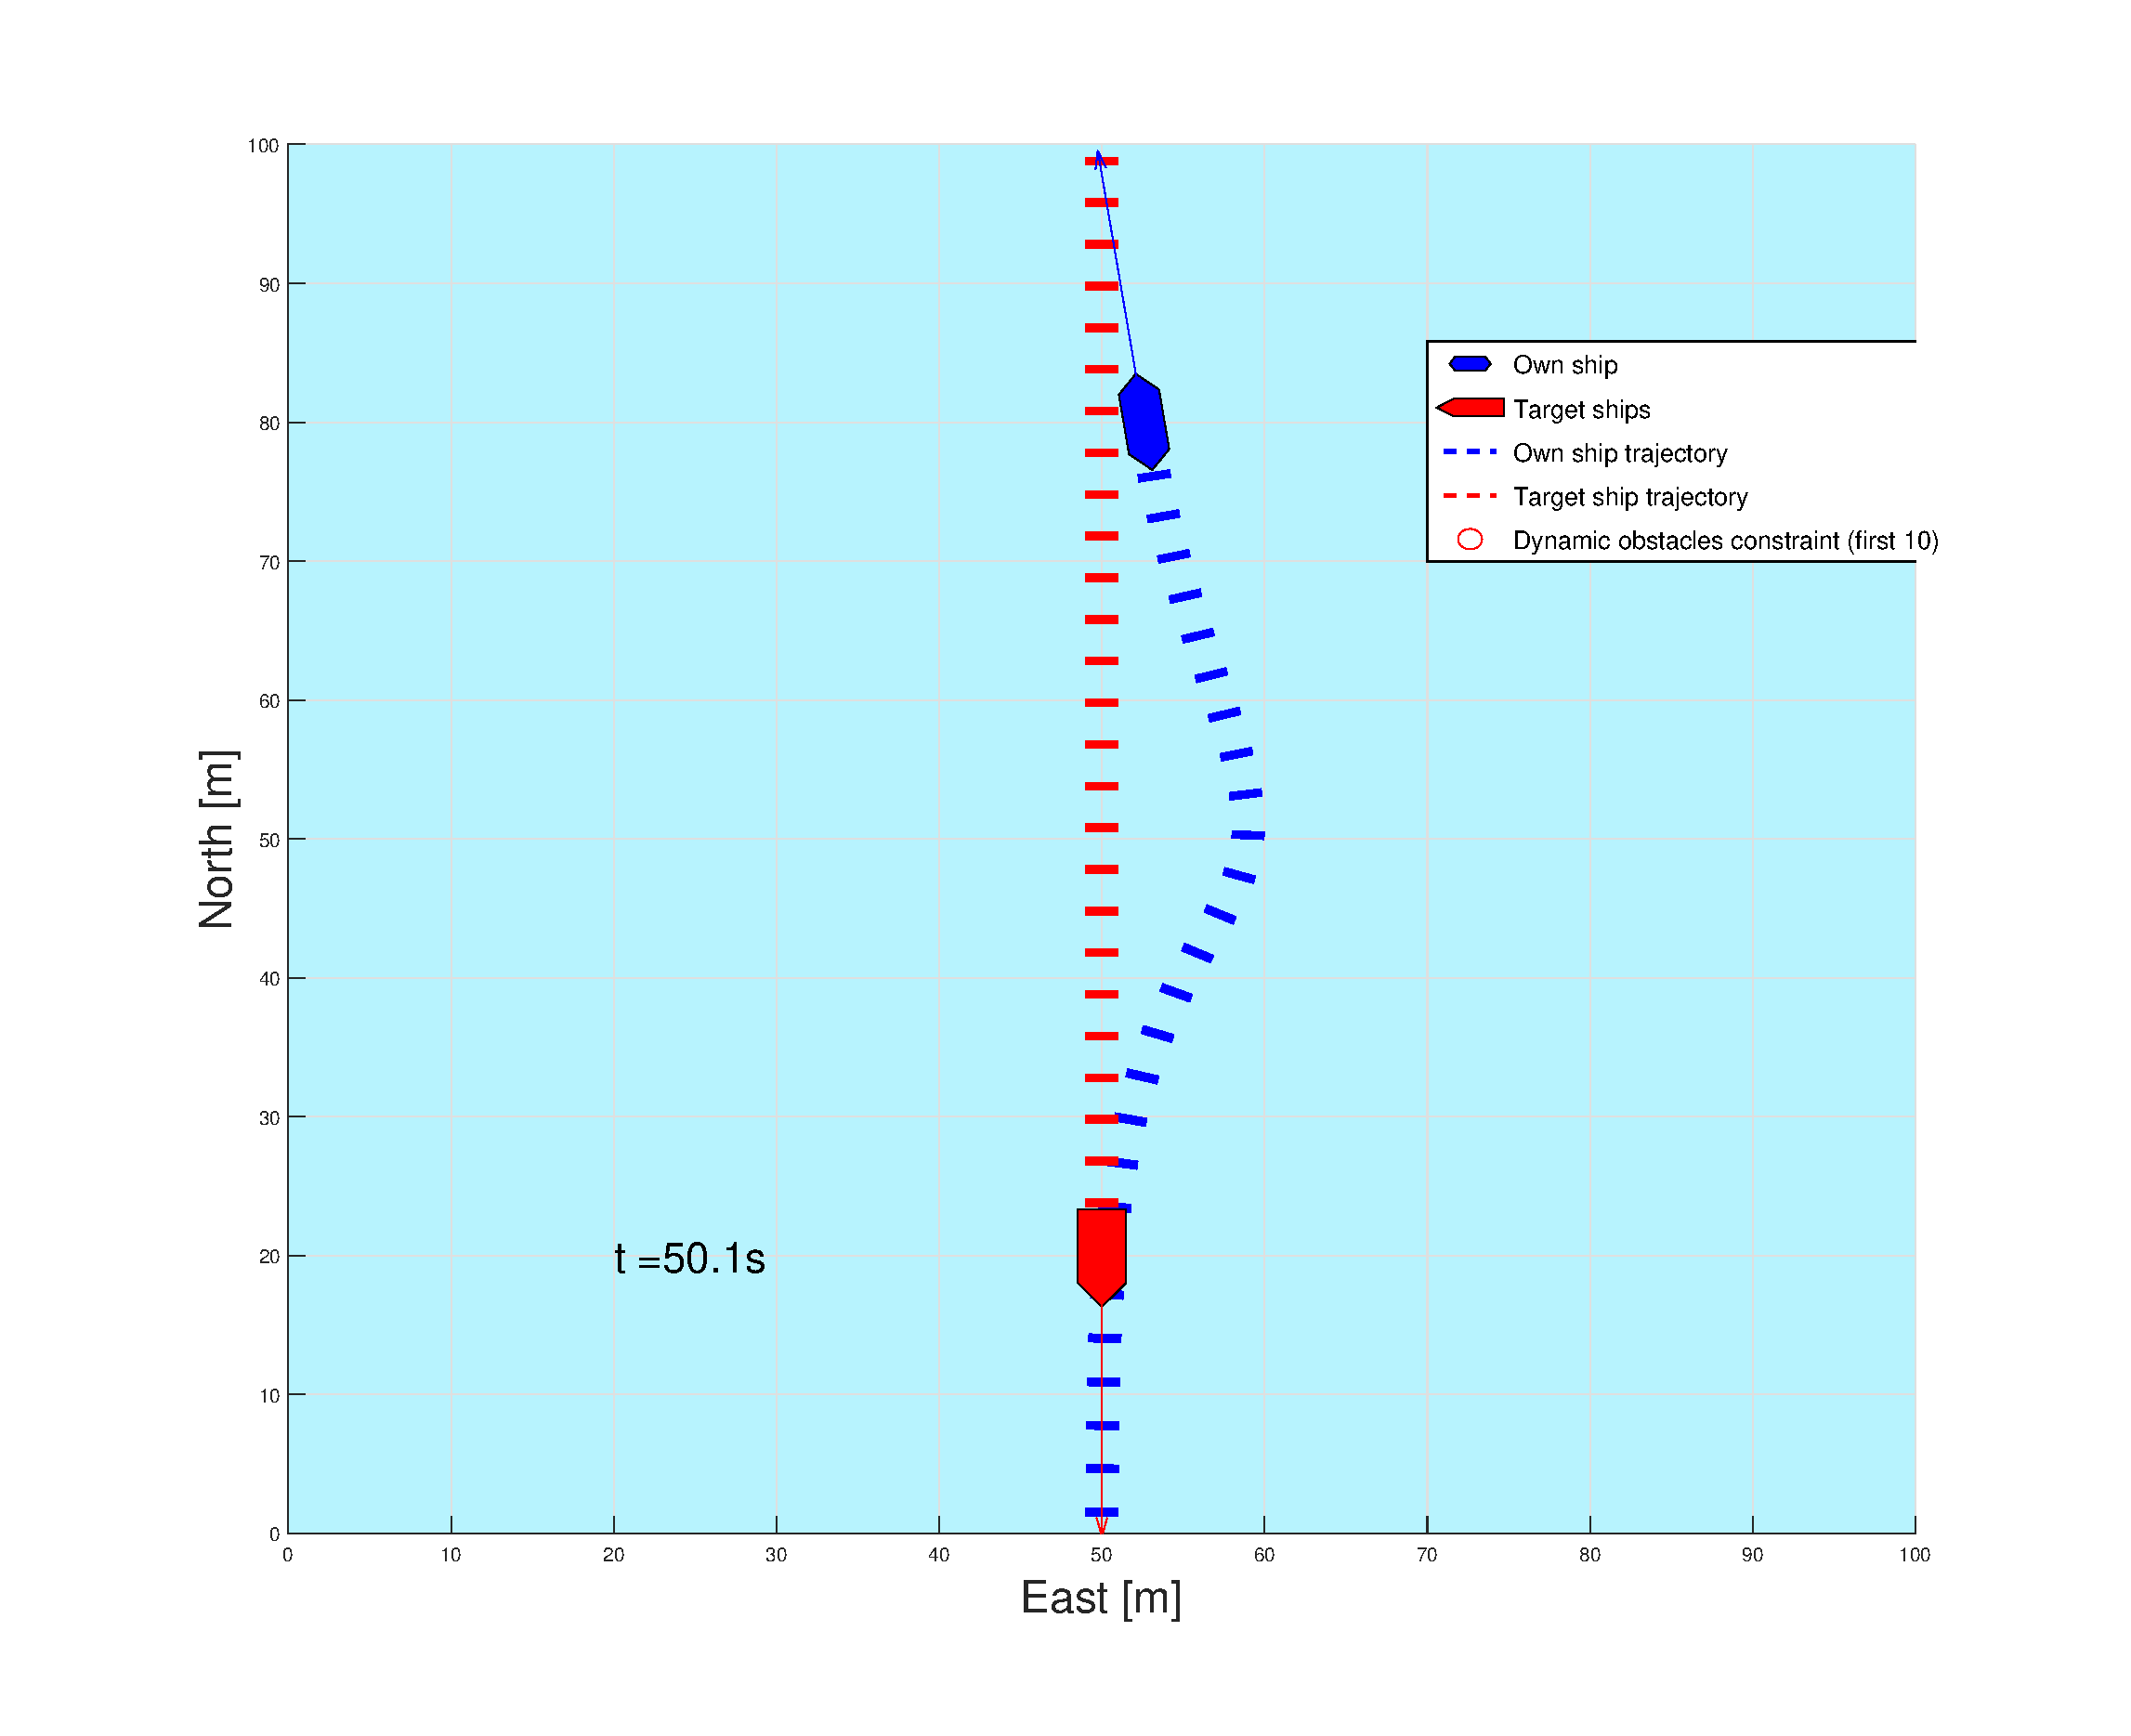
\includegraphics[width=\textwidth]{Images/Figures/enkel_HO/_Simple_1fig1_time=50}
%         \subcaption{}
%     \end{subfigure}
%     \hfill
%     \begin{subfigure}[b]{0.499\textwidth}
%         \centering
%         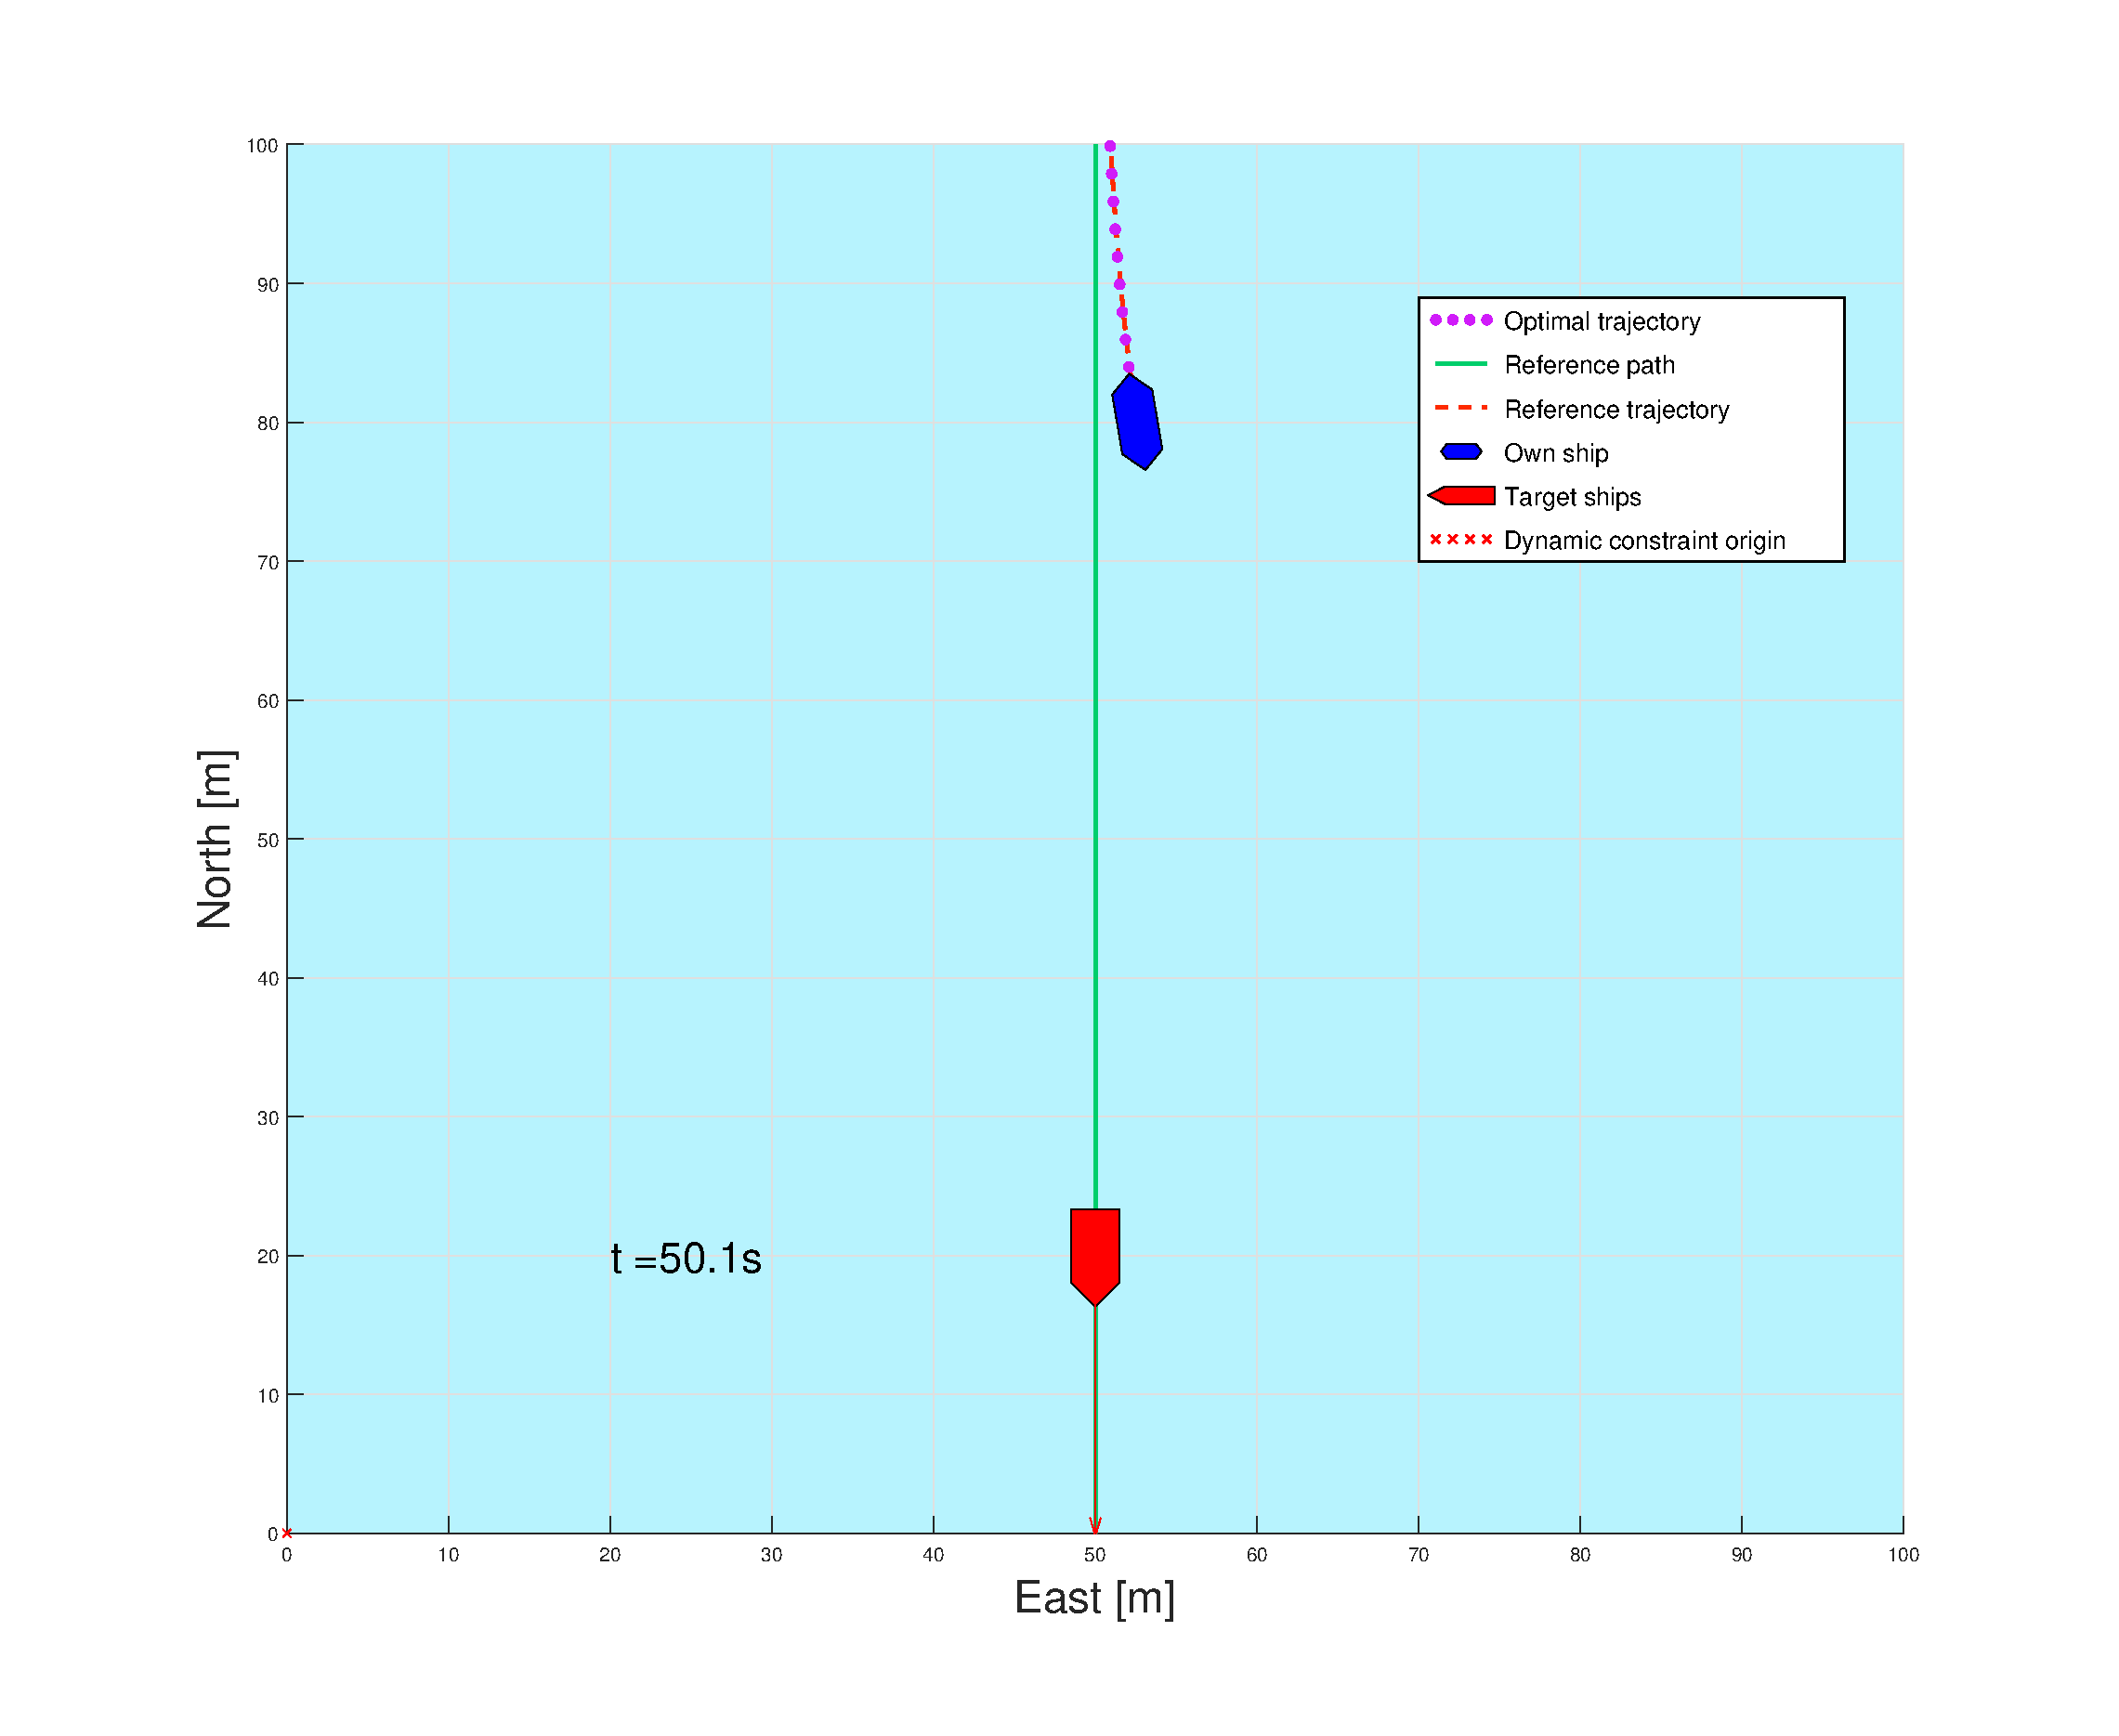
\includegraphics[width=\textwidth]{Images/Figures/enkel_HO/_Simple_1fig999_time=50}
%         \subcaption{}
%     \end{subfigure}
%     \hfill
%     \\
%     \begin{subfigure}[b]{0.49\textwidth}
%         \centering
%         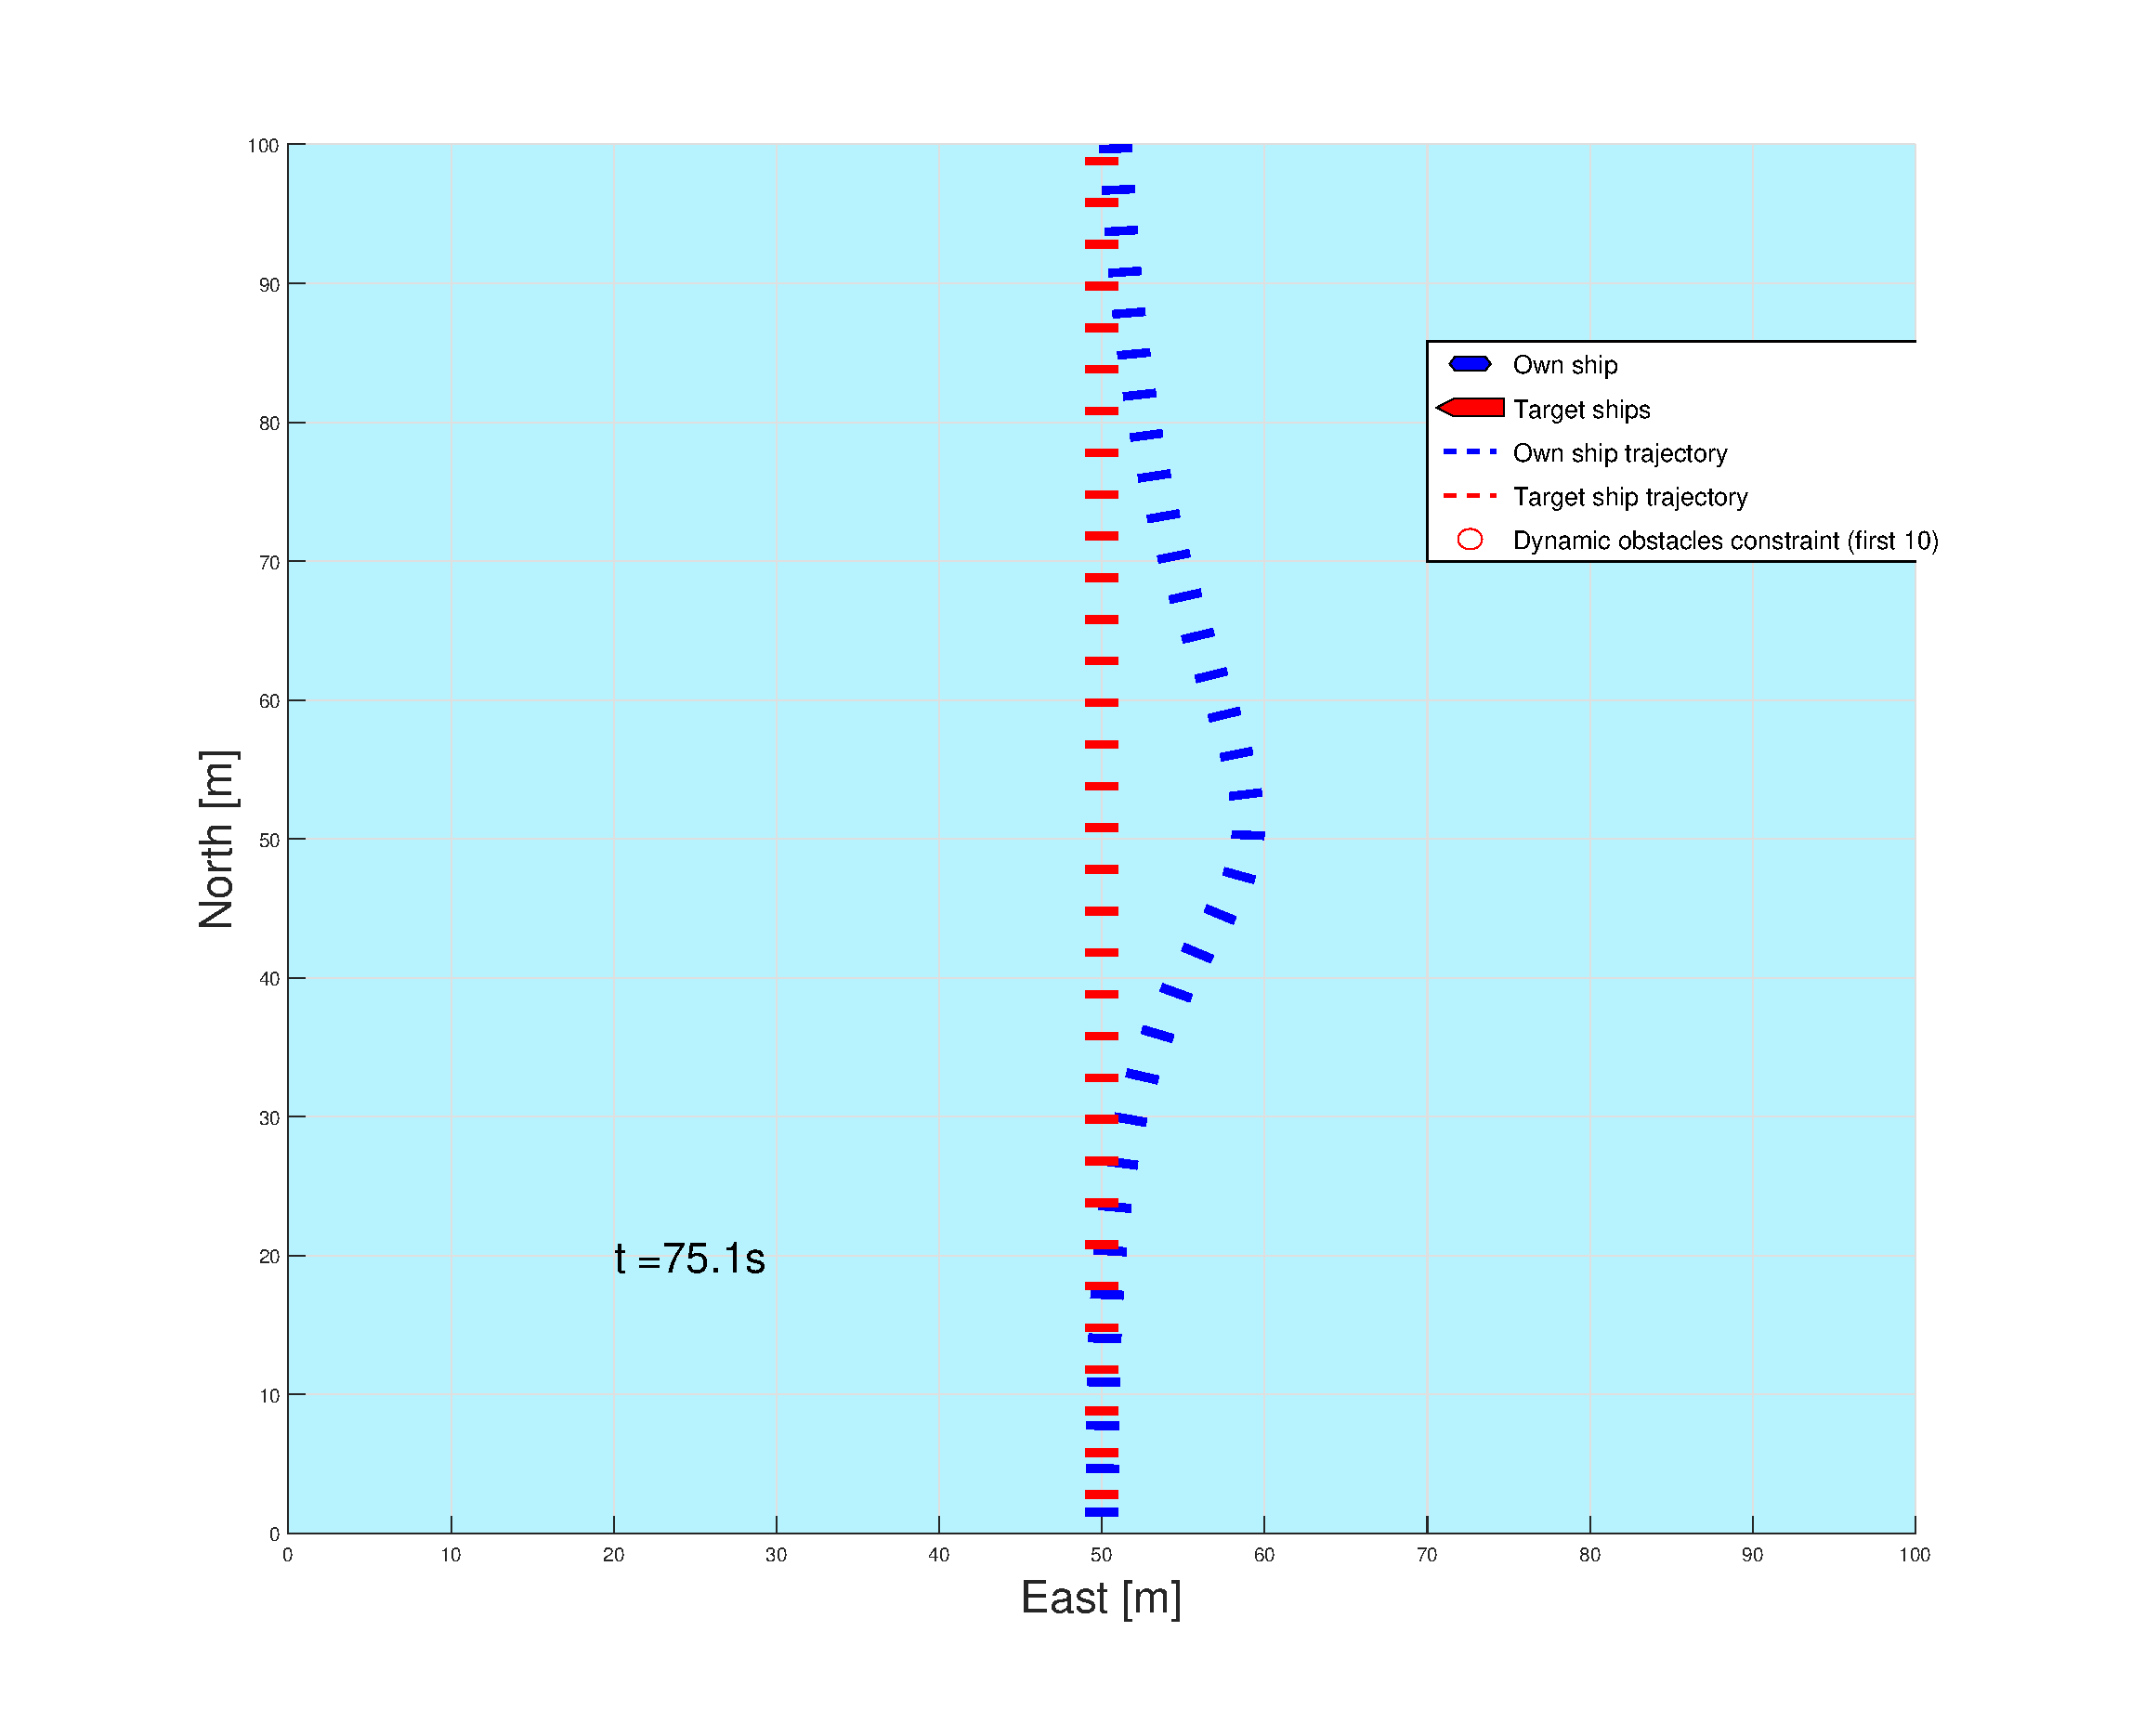
\includegraphics[width=\textwidth]{Images/Figures/enkel_HO/_Simple_1fig1_time=75}
%         \subcaption{}
%     \end{subfigure}
%     \hfill
%     \begin{subfigure}[b]{0.499\textwidth}
%         \centering
%         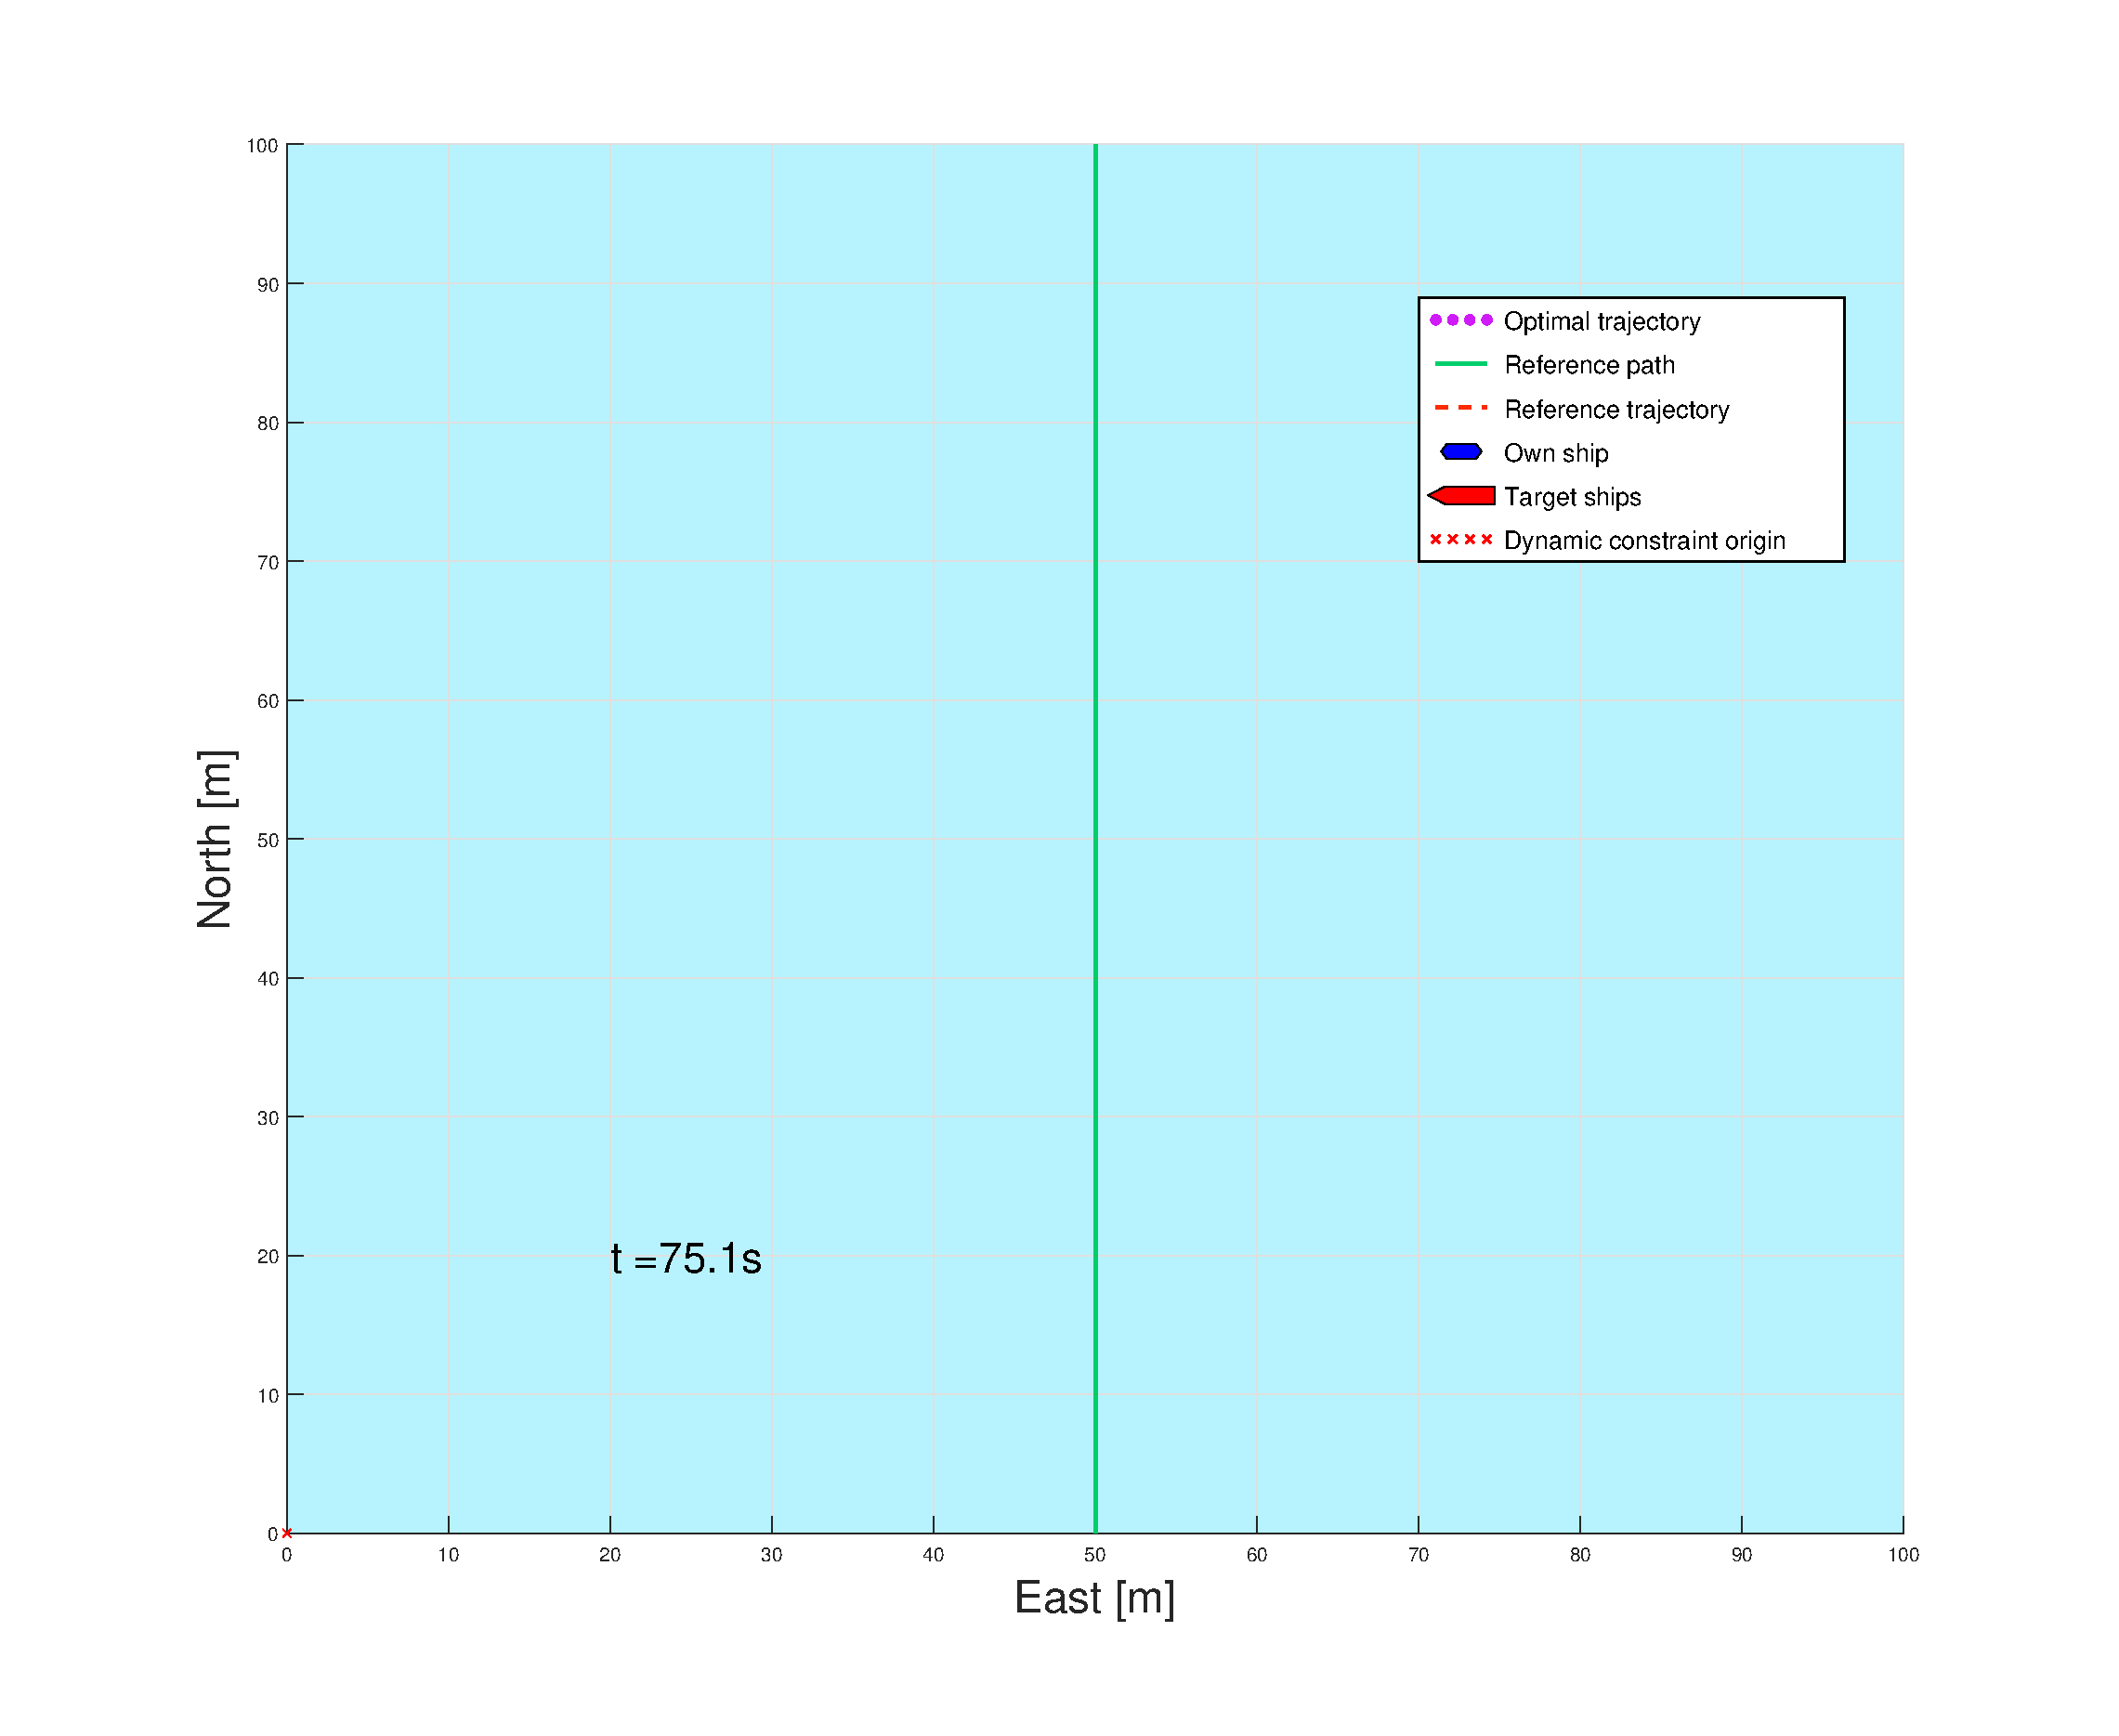
\includegraphics[width=\textwidth]{Images/Figures/enkel_HO/_Simple_1fig999_time=75}
%         \subcaption{}
%     \end{subfigure}
%     \hfill
%     \caption{Simple Head on Without Prediction}
% \end{figure}

\begin{figure}[ht!] % SIMPLE GIVE WAY
    % \begin{subfigure}[b]{0.49\textwidth}
    %     \centering
    %     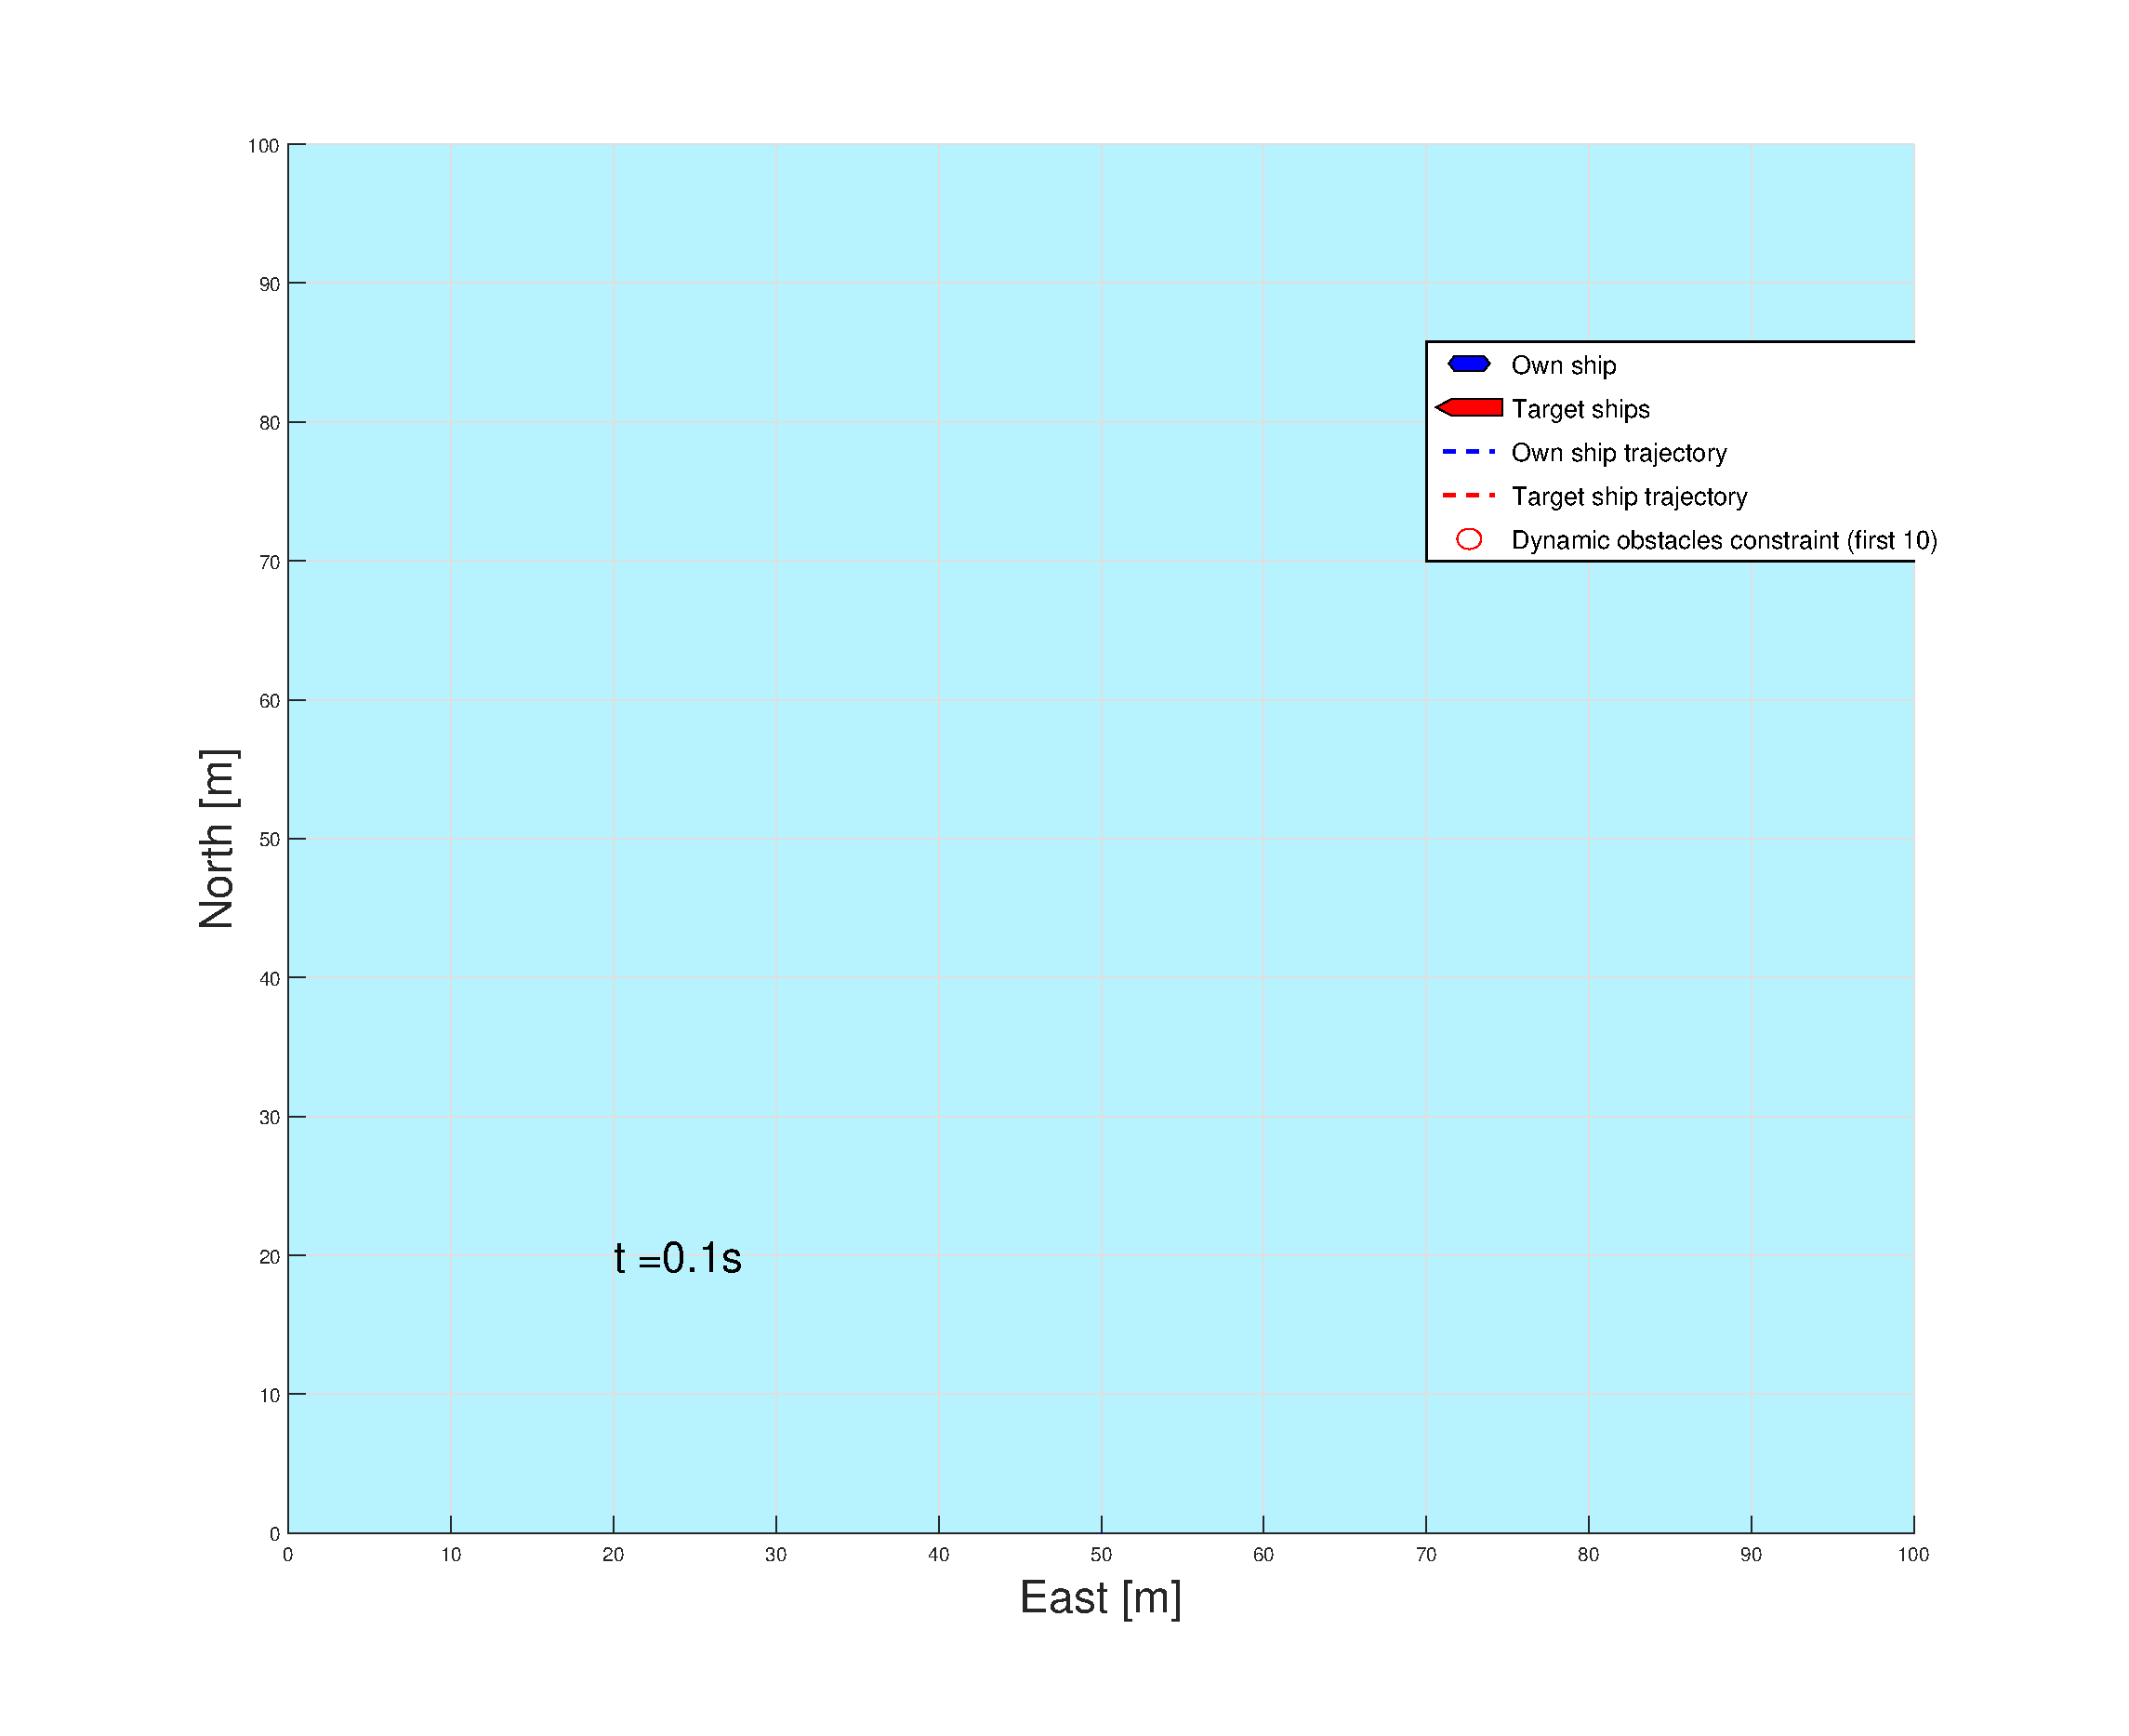
\includegraphics[width=\textwidth]{Images/Figures/enkel_GW/_Simple_0fig1_time=0}
    %     \subcaption{}
    % \end{subfigure}
    % \hfill
    % \begin{subfigure}[b]{0.499\textwidth}
    %     \centering
    %     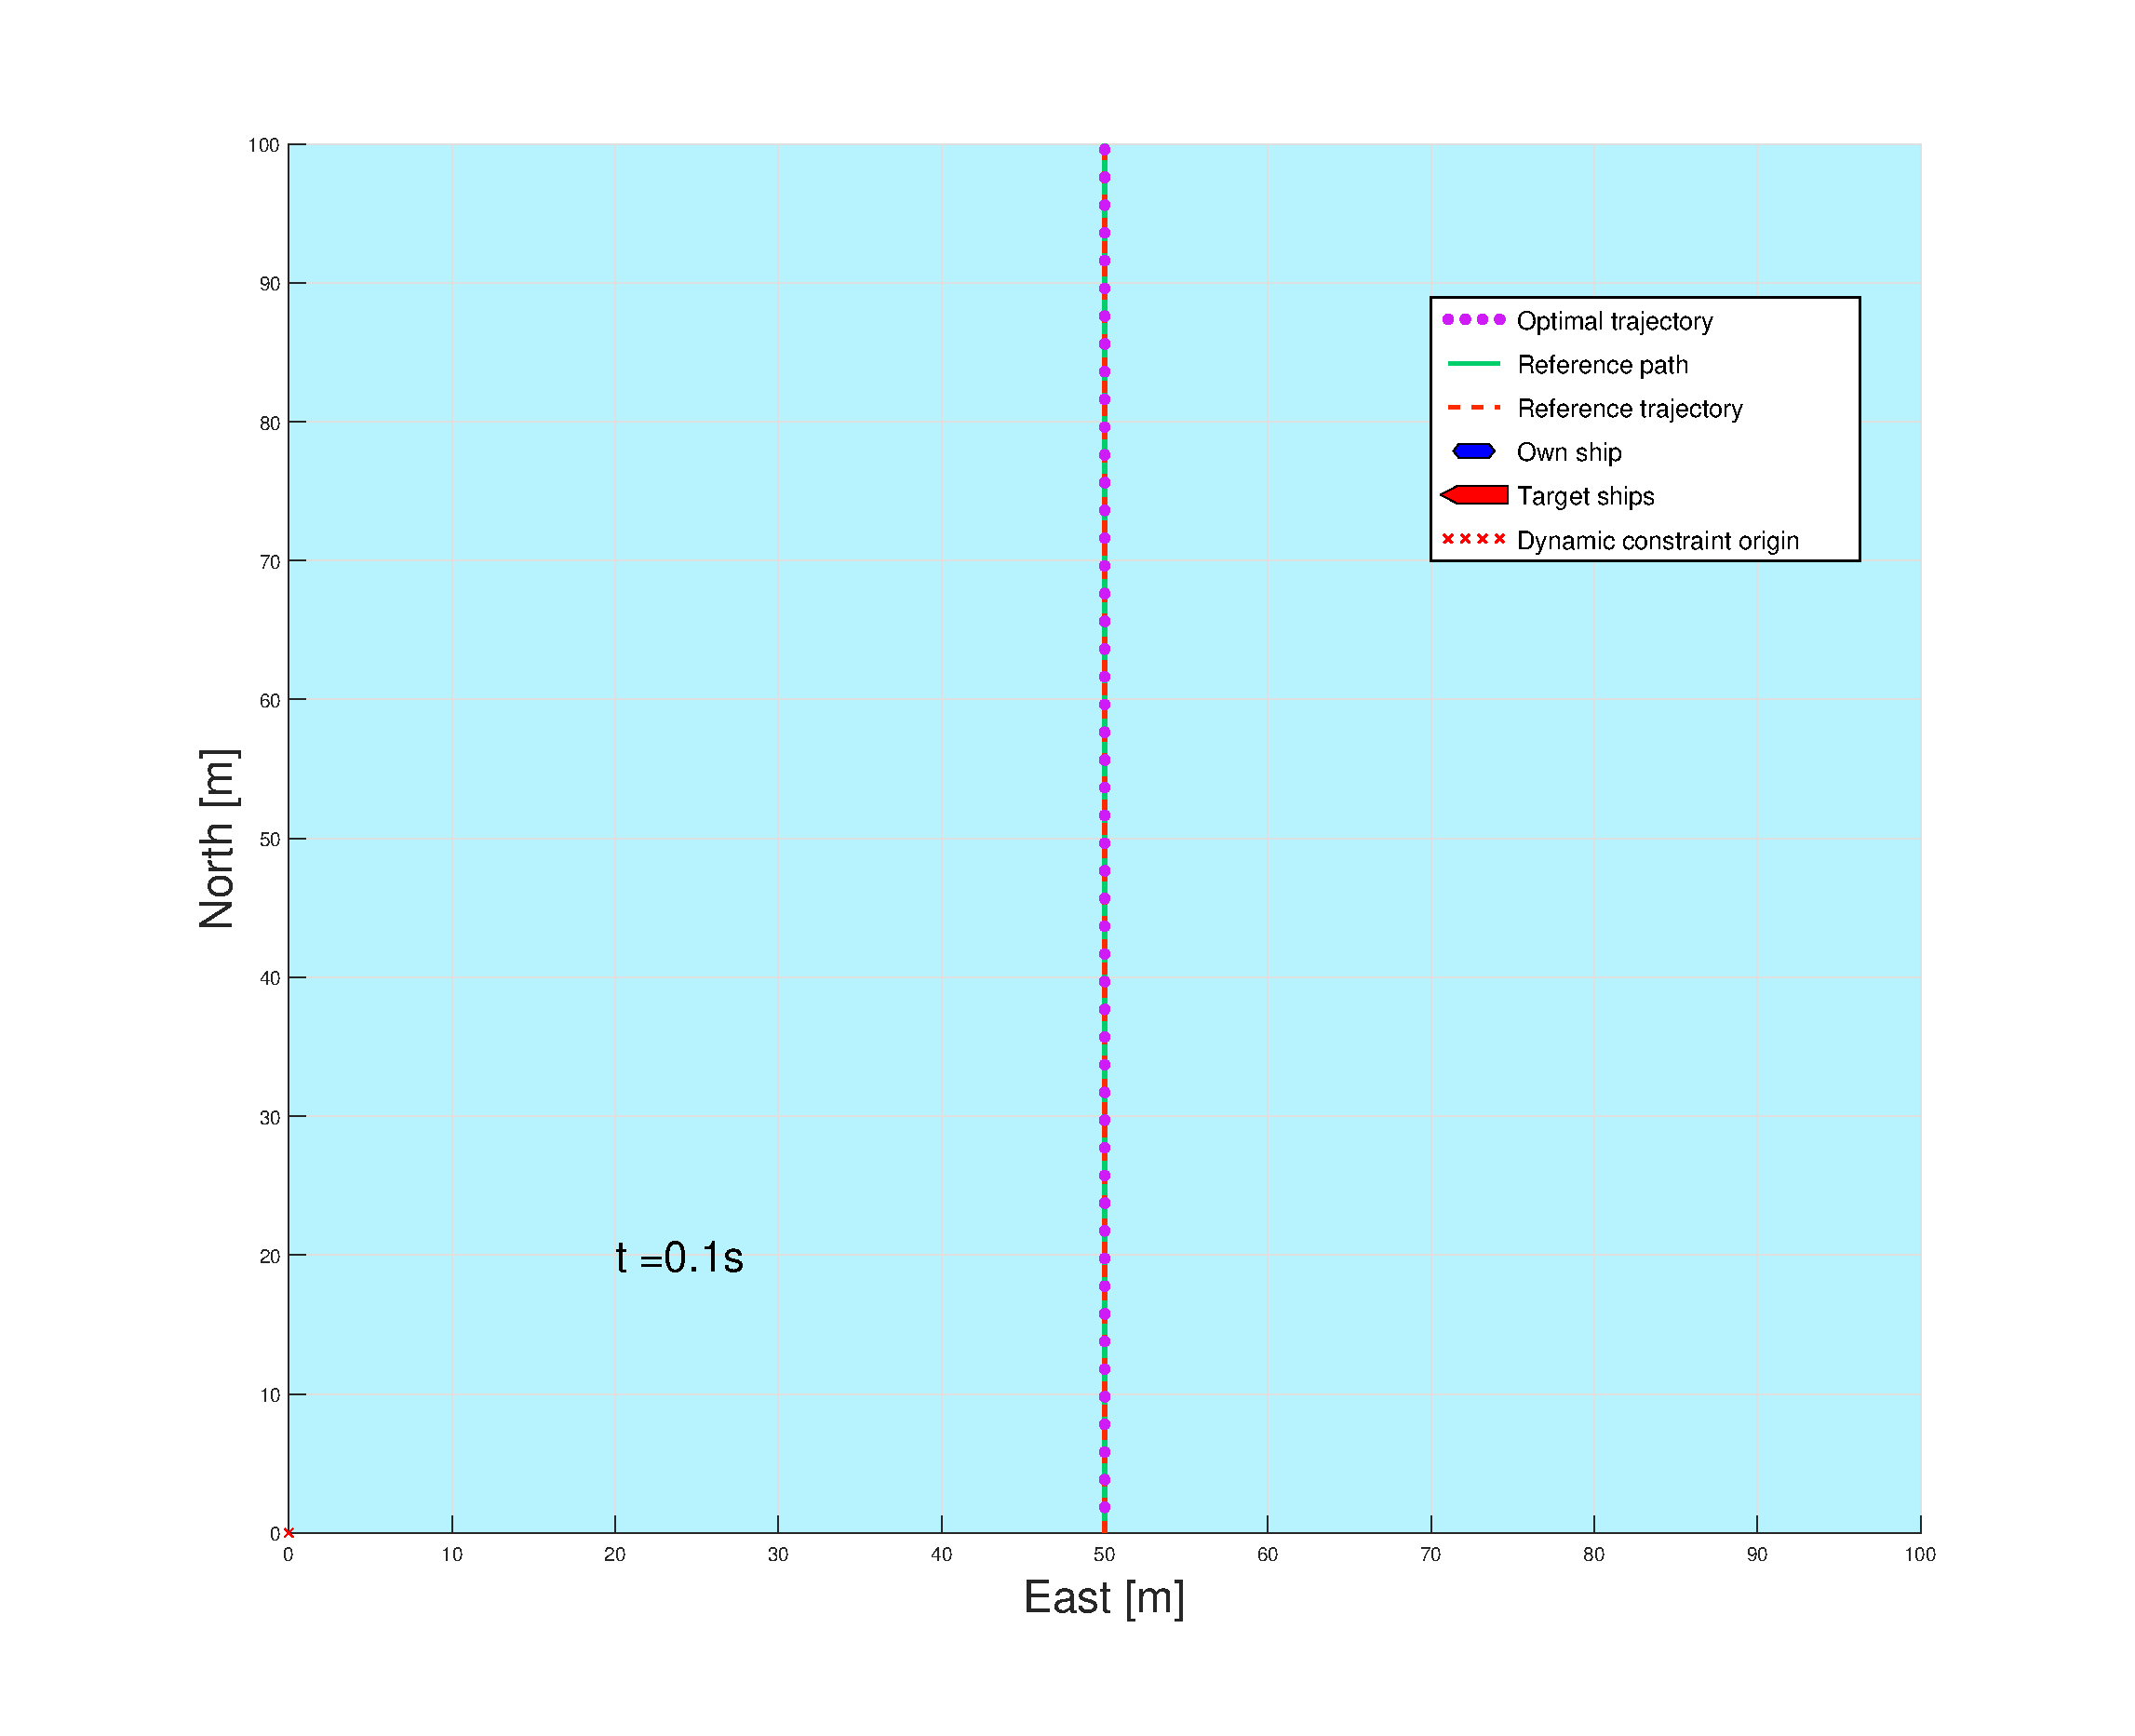
\includegraphics[width=\textwidth]{Images/Figures/enkel_GW/_Simple_0fig999_time=0}
    %     \subcaption{}
    % \end{subfigure}
    % \hfill
    % \\
    \begin{subfigure}[b]{0.49\textwidth}
        \centering
        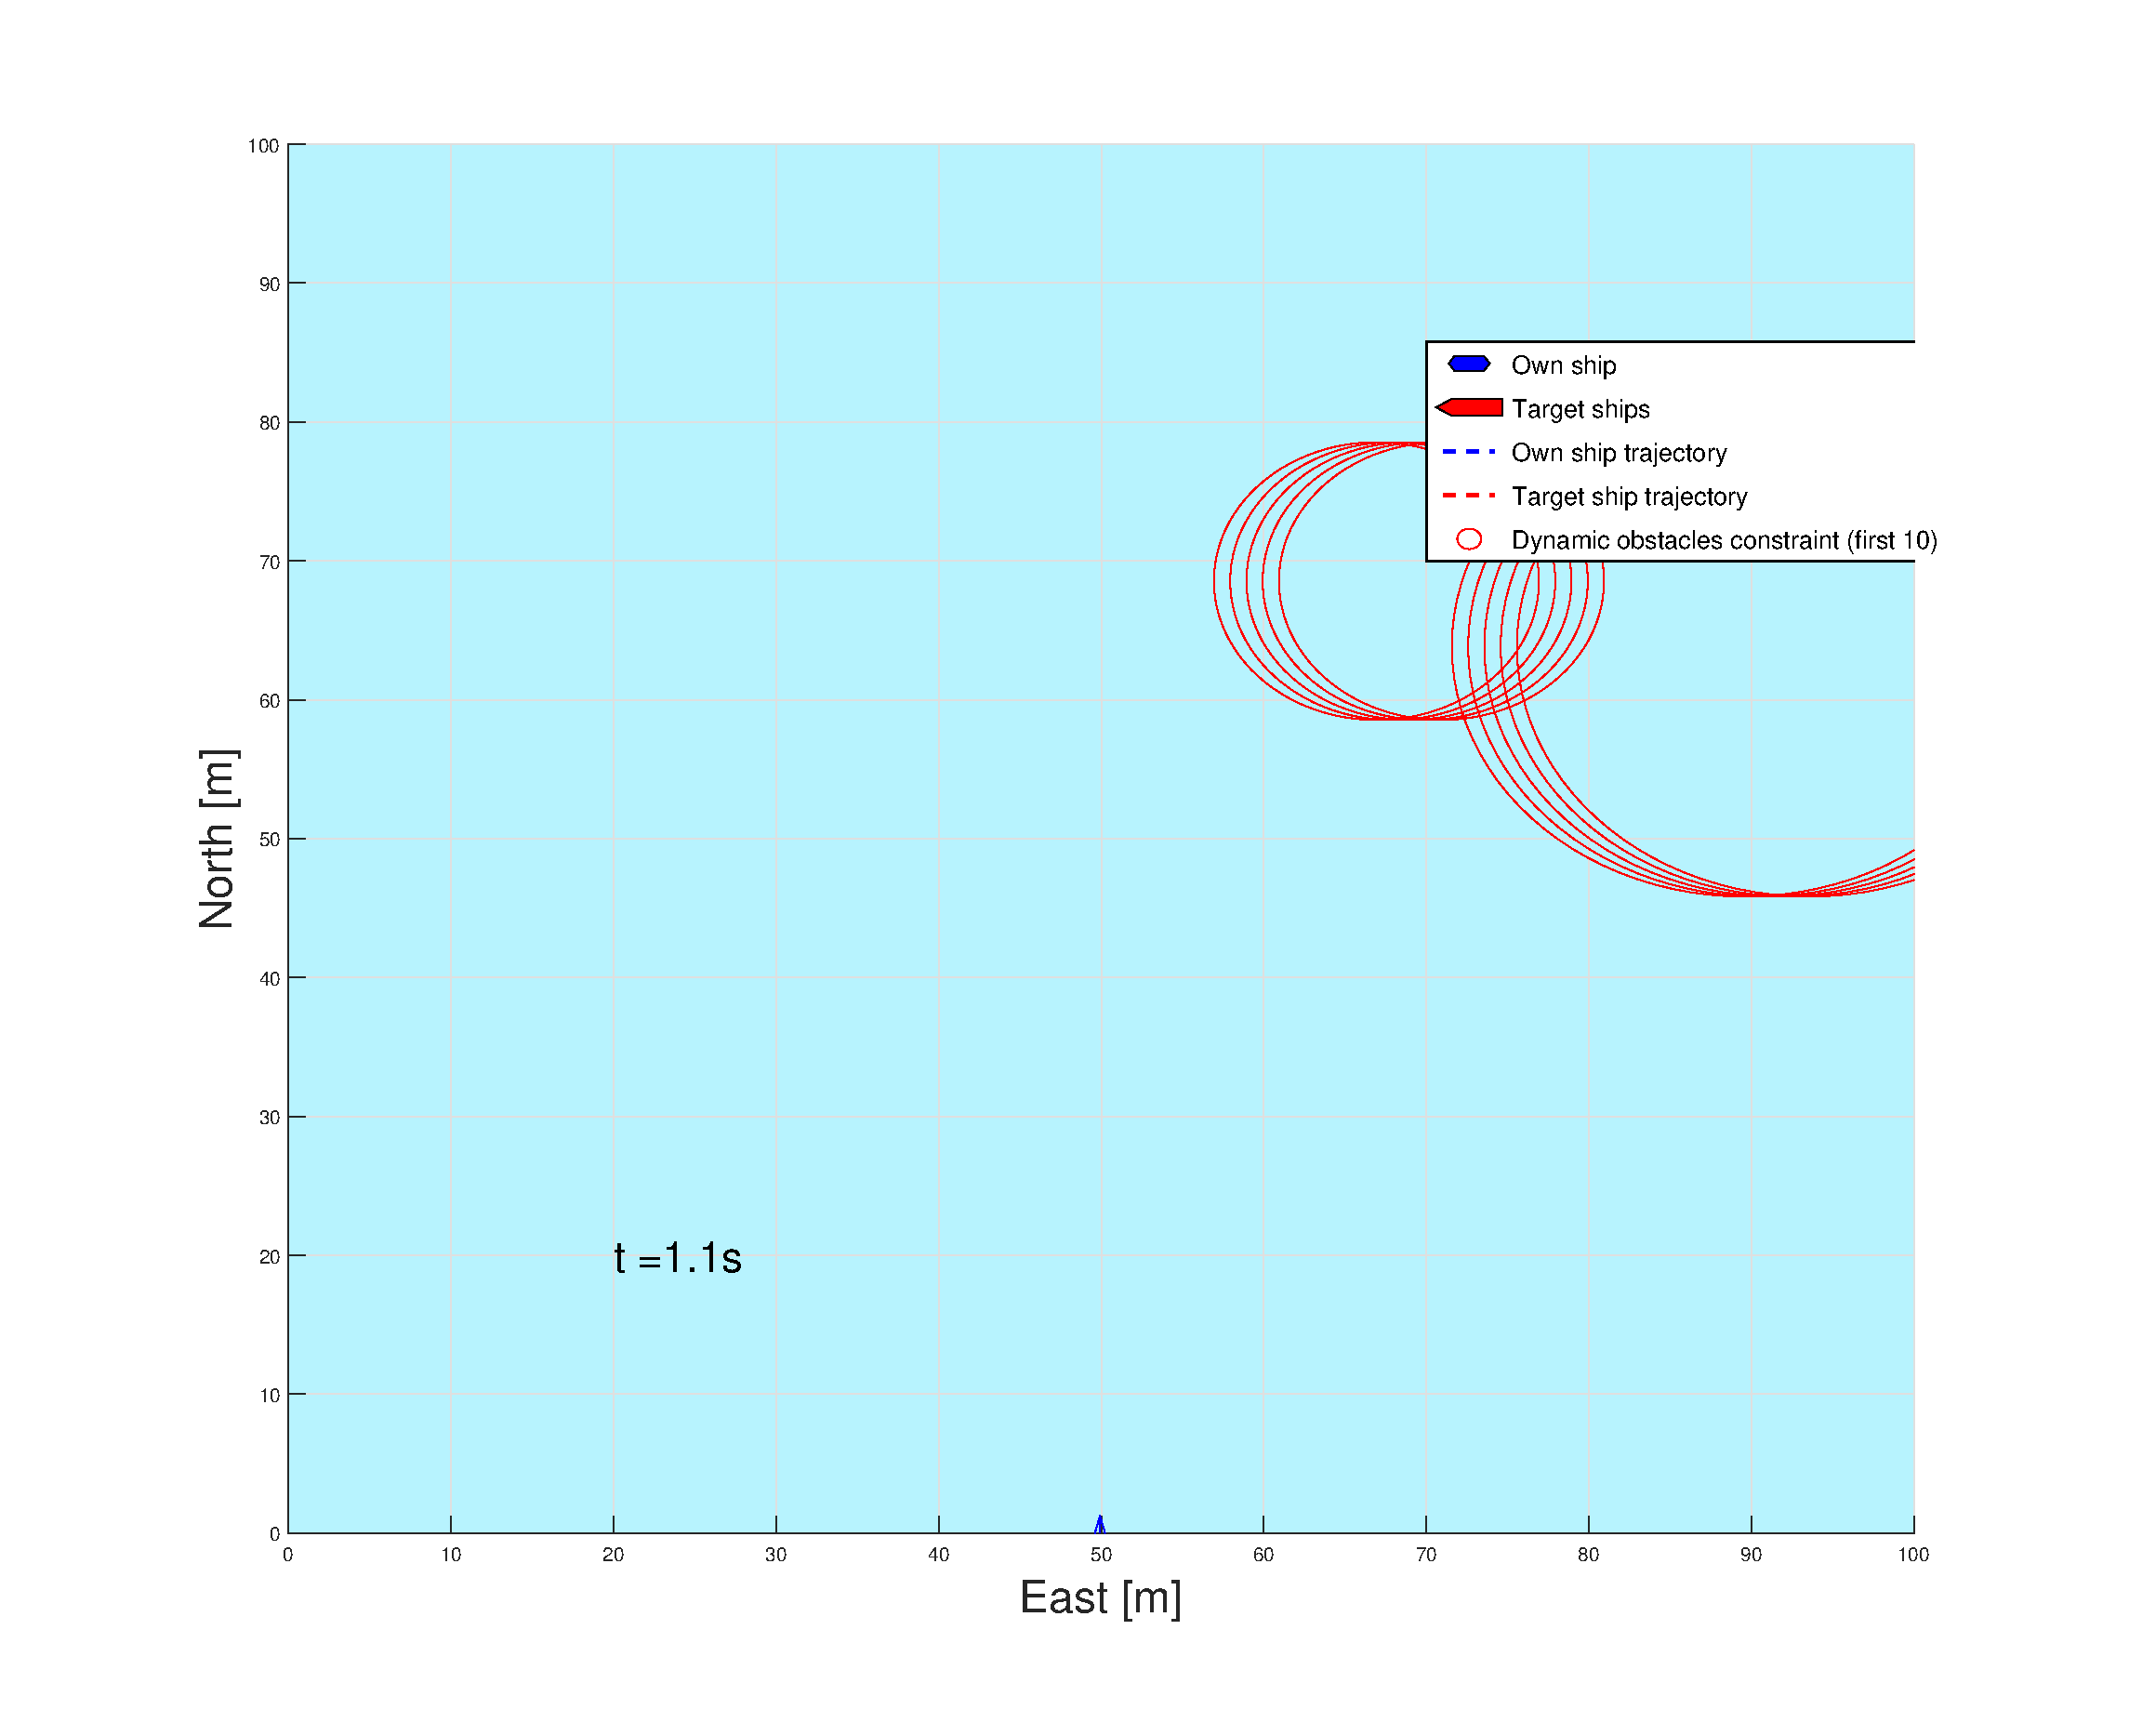
\includegraphics[width=\textwidth]{Images/Figures/enkel_GW/_Simple_0fig1_time=1}
        \subcaption{}
    \end{subfigure}
    \hfill
    \begin{subfigure}[b]{0.499\textwidth}
        \centering
        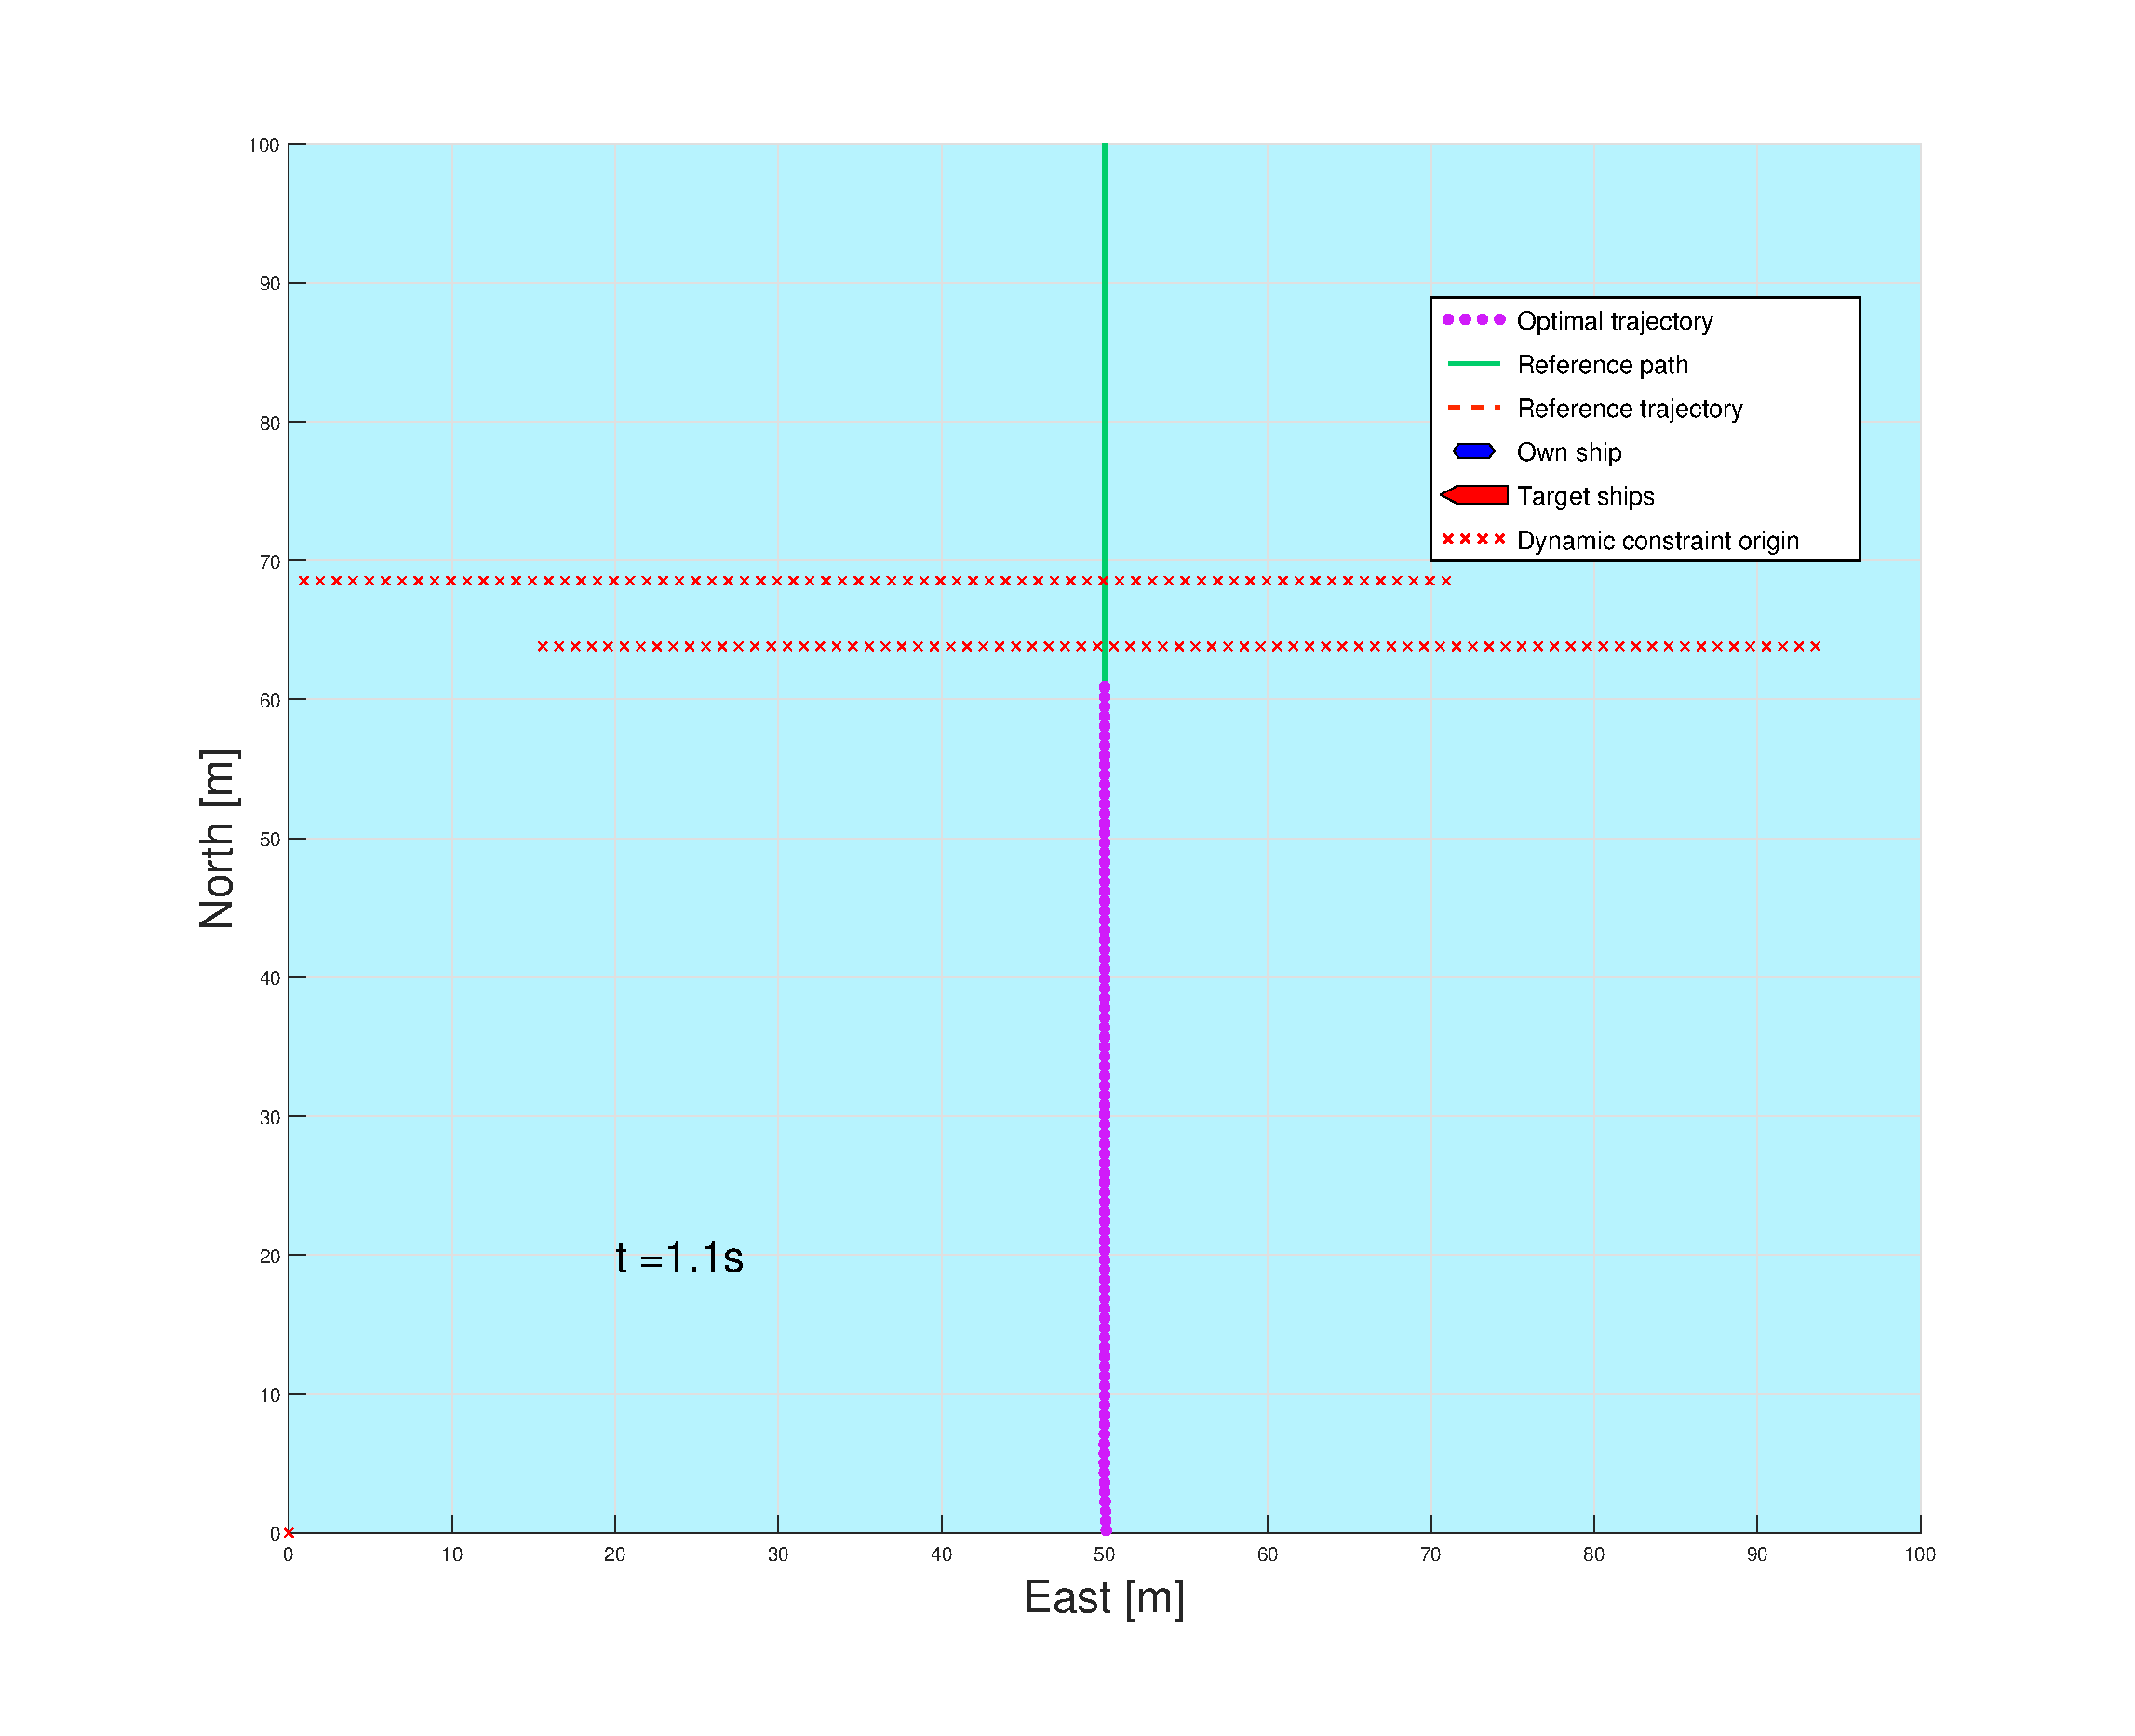
\includegraphics[width=\textwidth]{Images/Figures/enkel_GW/_Simple_0fig999_time=1}
        \subcaption{}
    \end{subfigure}
    \hfill
    \\
    \begin{subfigure}[b]{0.49\textwidth}
        \centering
        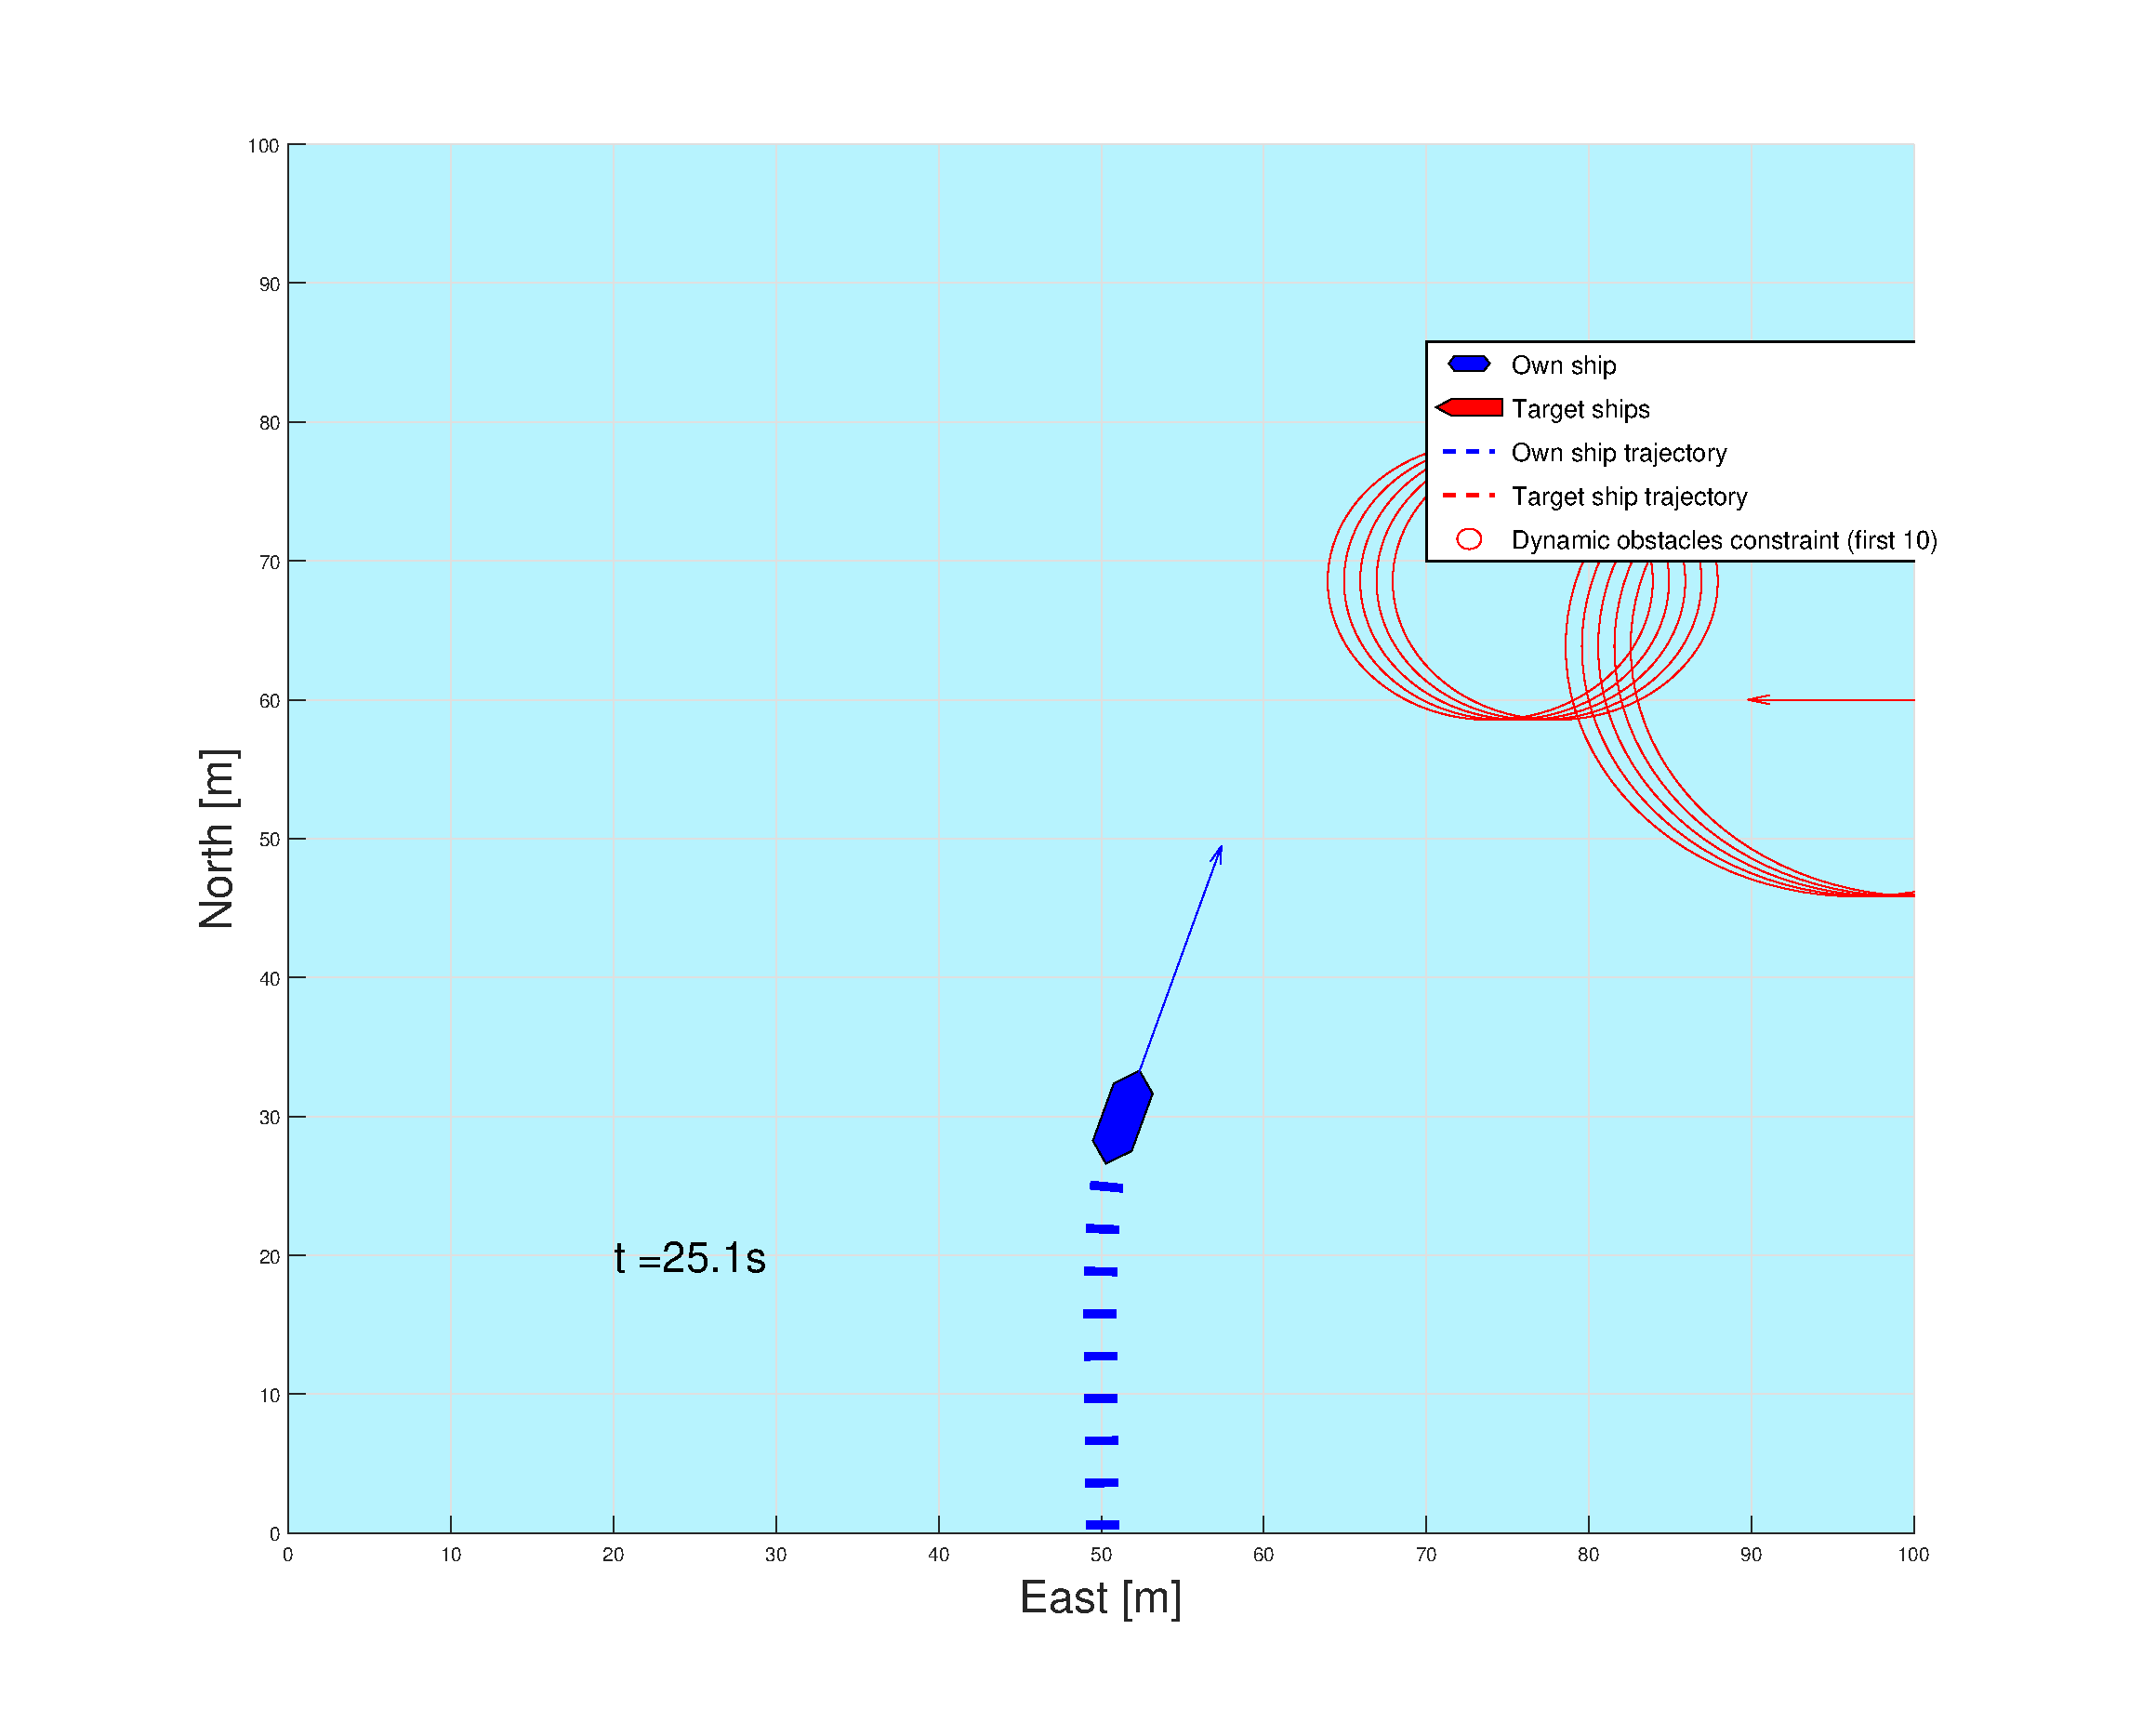
\includegraphics[width=\textwidth]{Images/Figures/enkel_GW/_Simple_0fig1_time=25}
        \subcaption{}
    \end{subfigure}
    \hfill
    \begin{subfigure}[b]{0.499\textwidth}
        \centering
        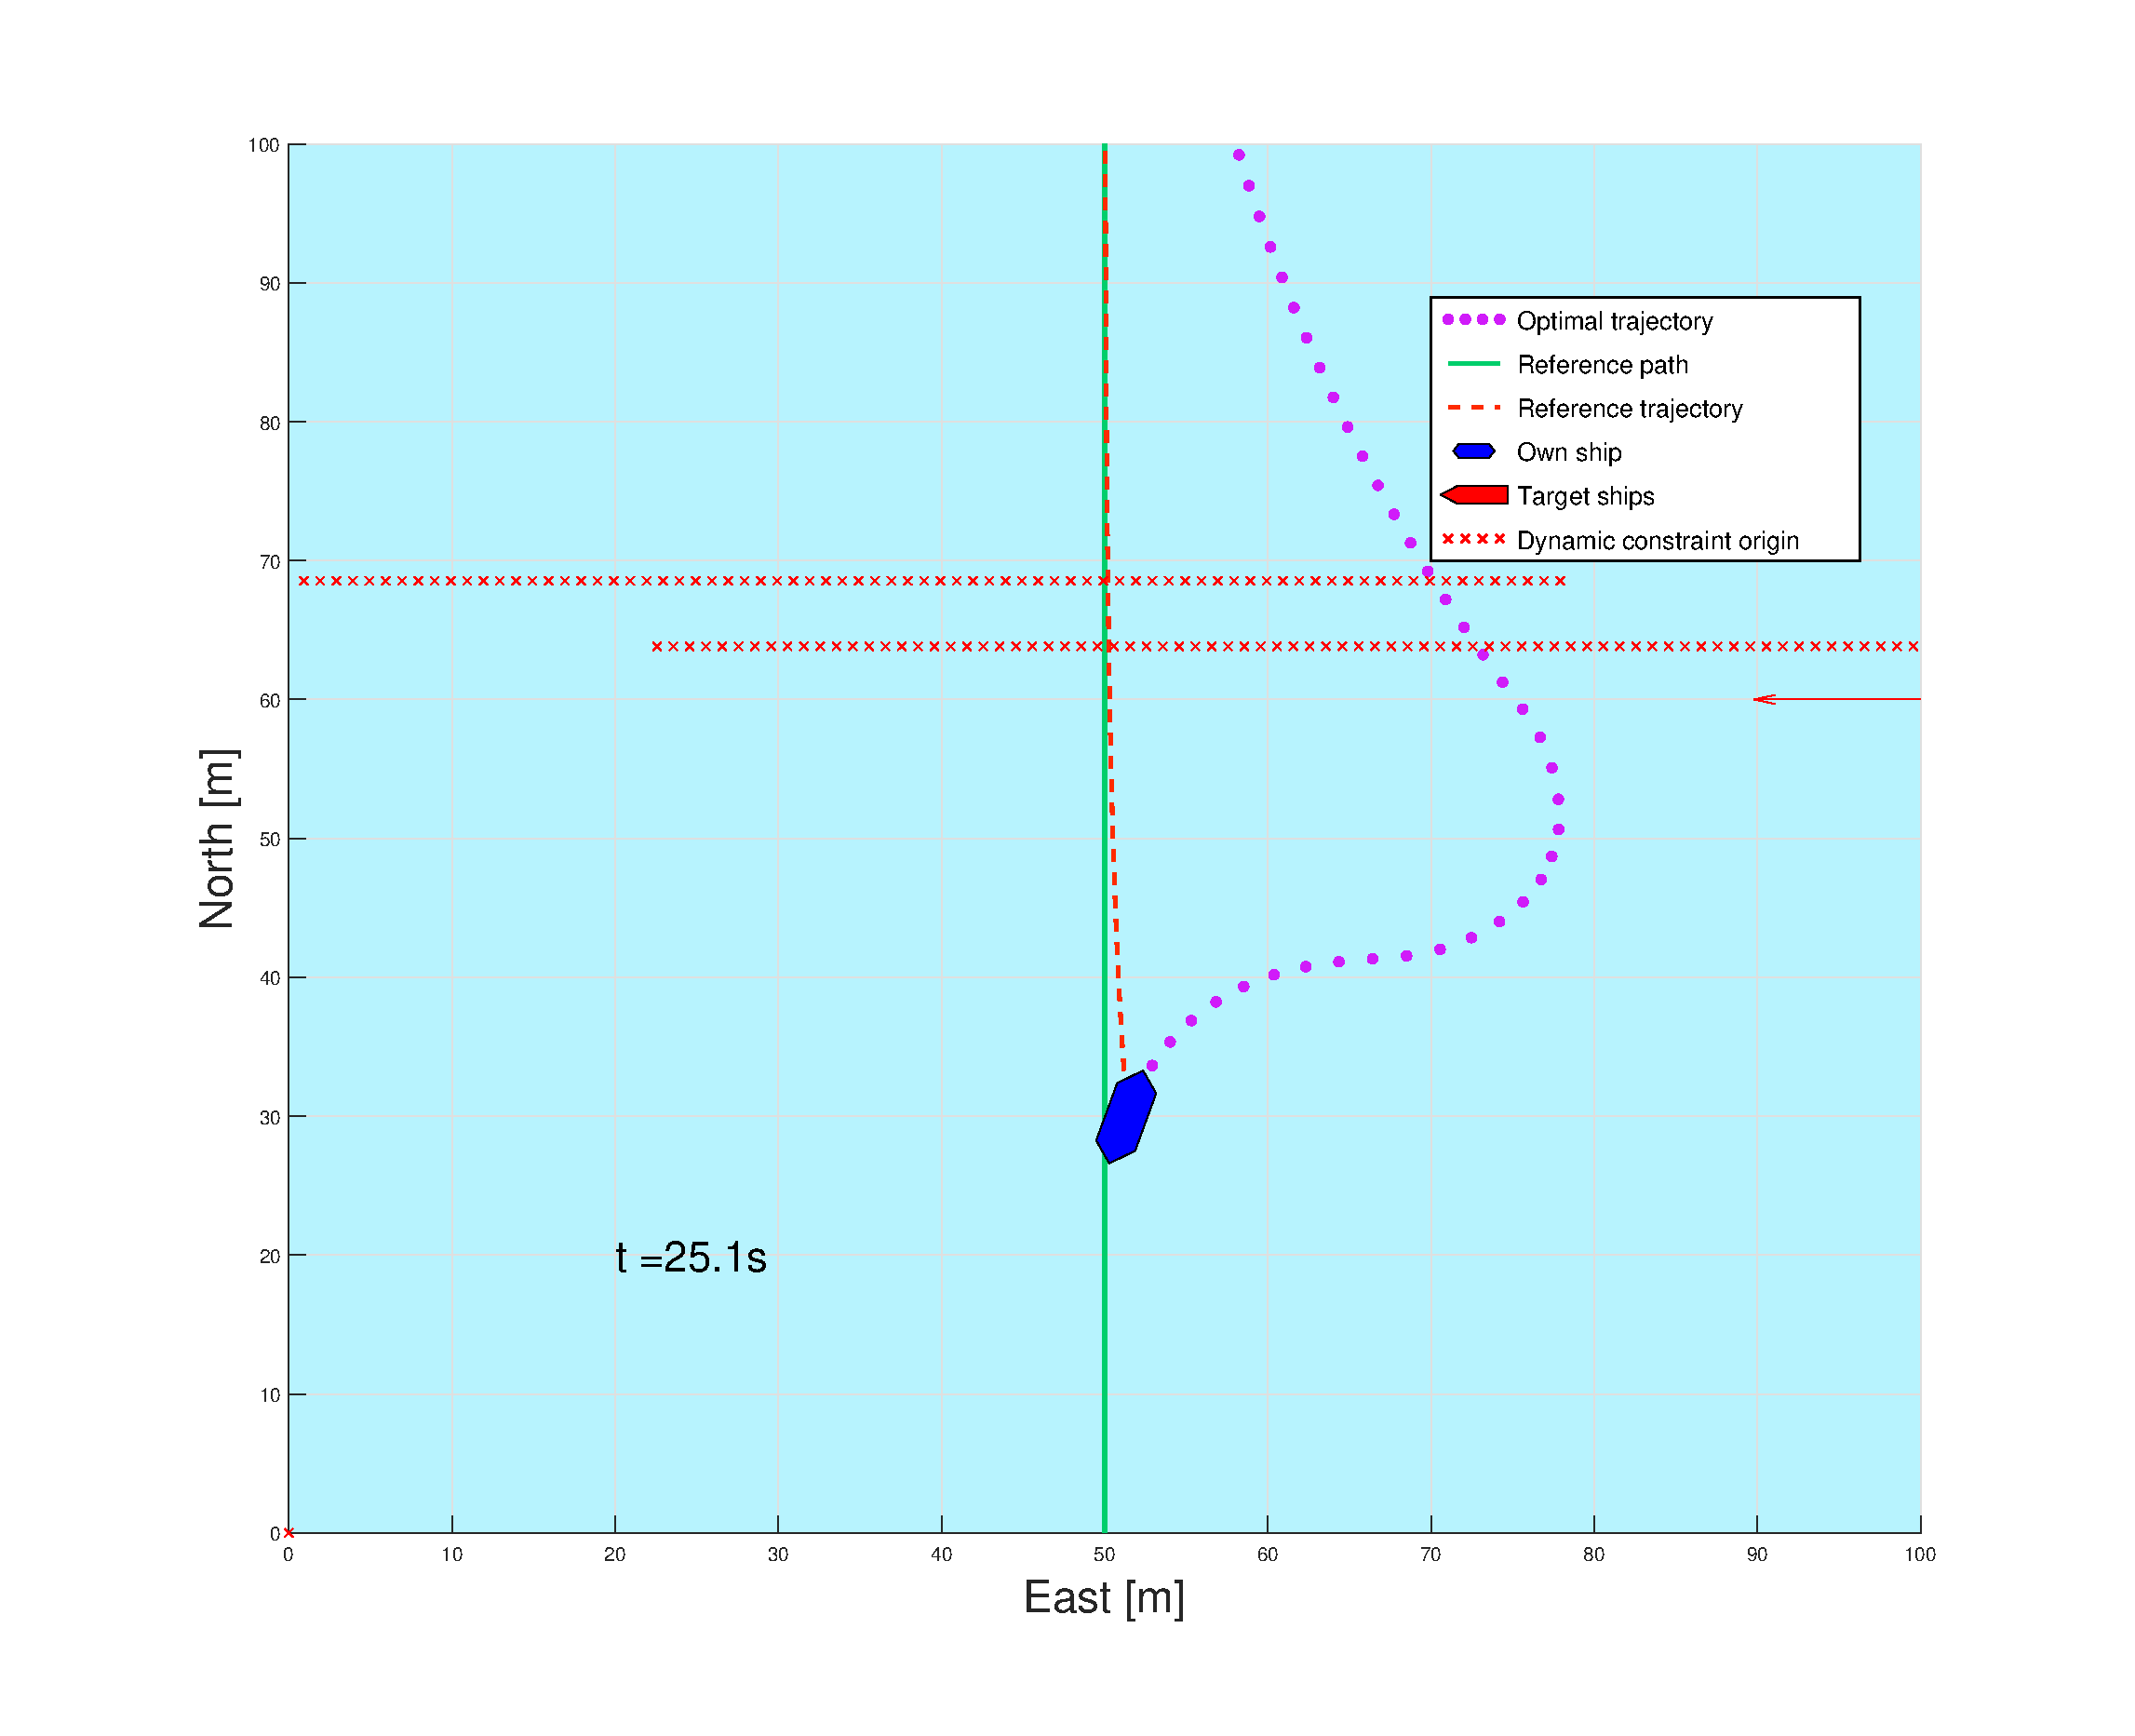
\includegraphics[width=\textwidth]{Images/Figures/enkel_GW/_Simple_0fig999_time=25}
        \subcaption{}
    \end{subfigure}
    \hfill
    \\
    \begin{subfigure}[b]{0.49\textwidth}
        \centering
        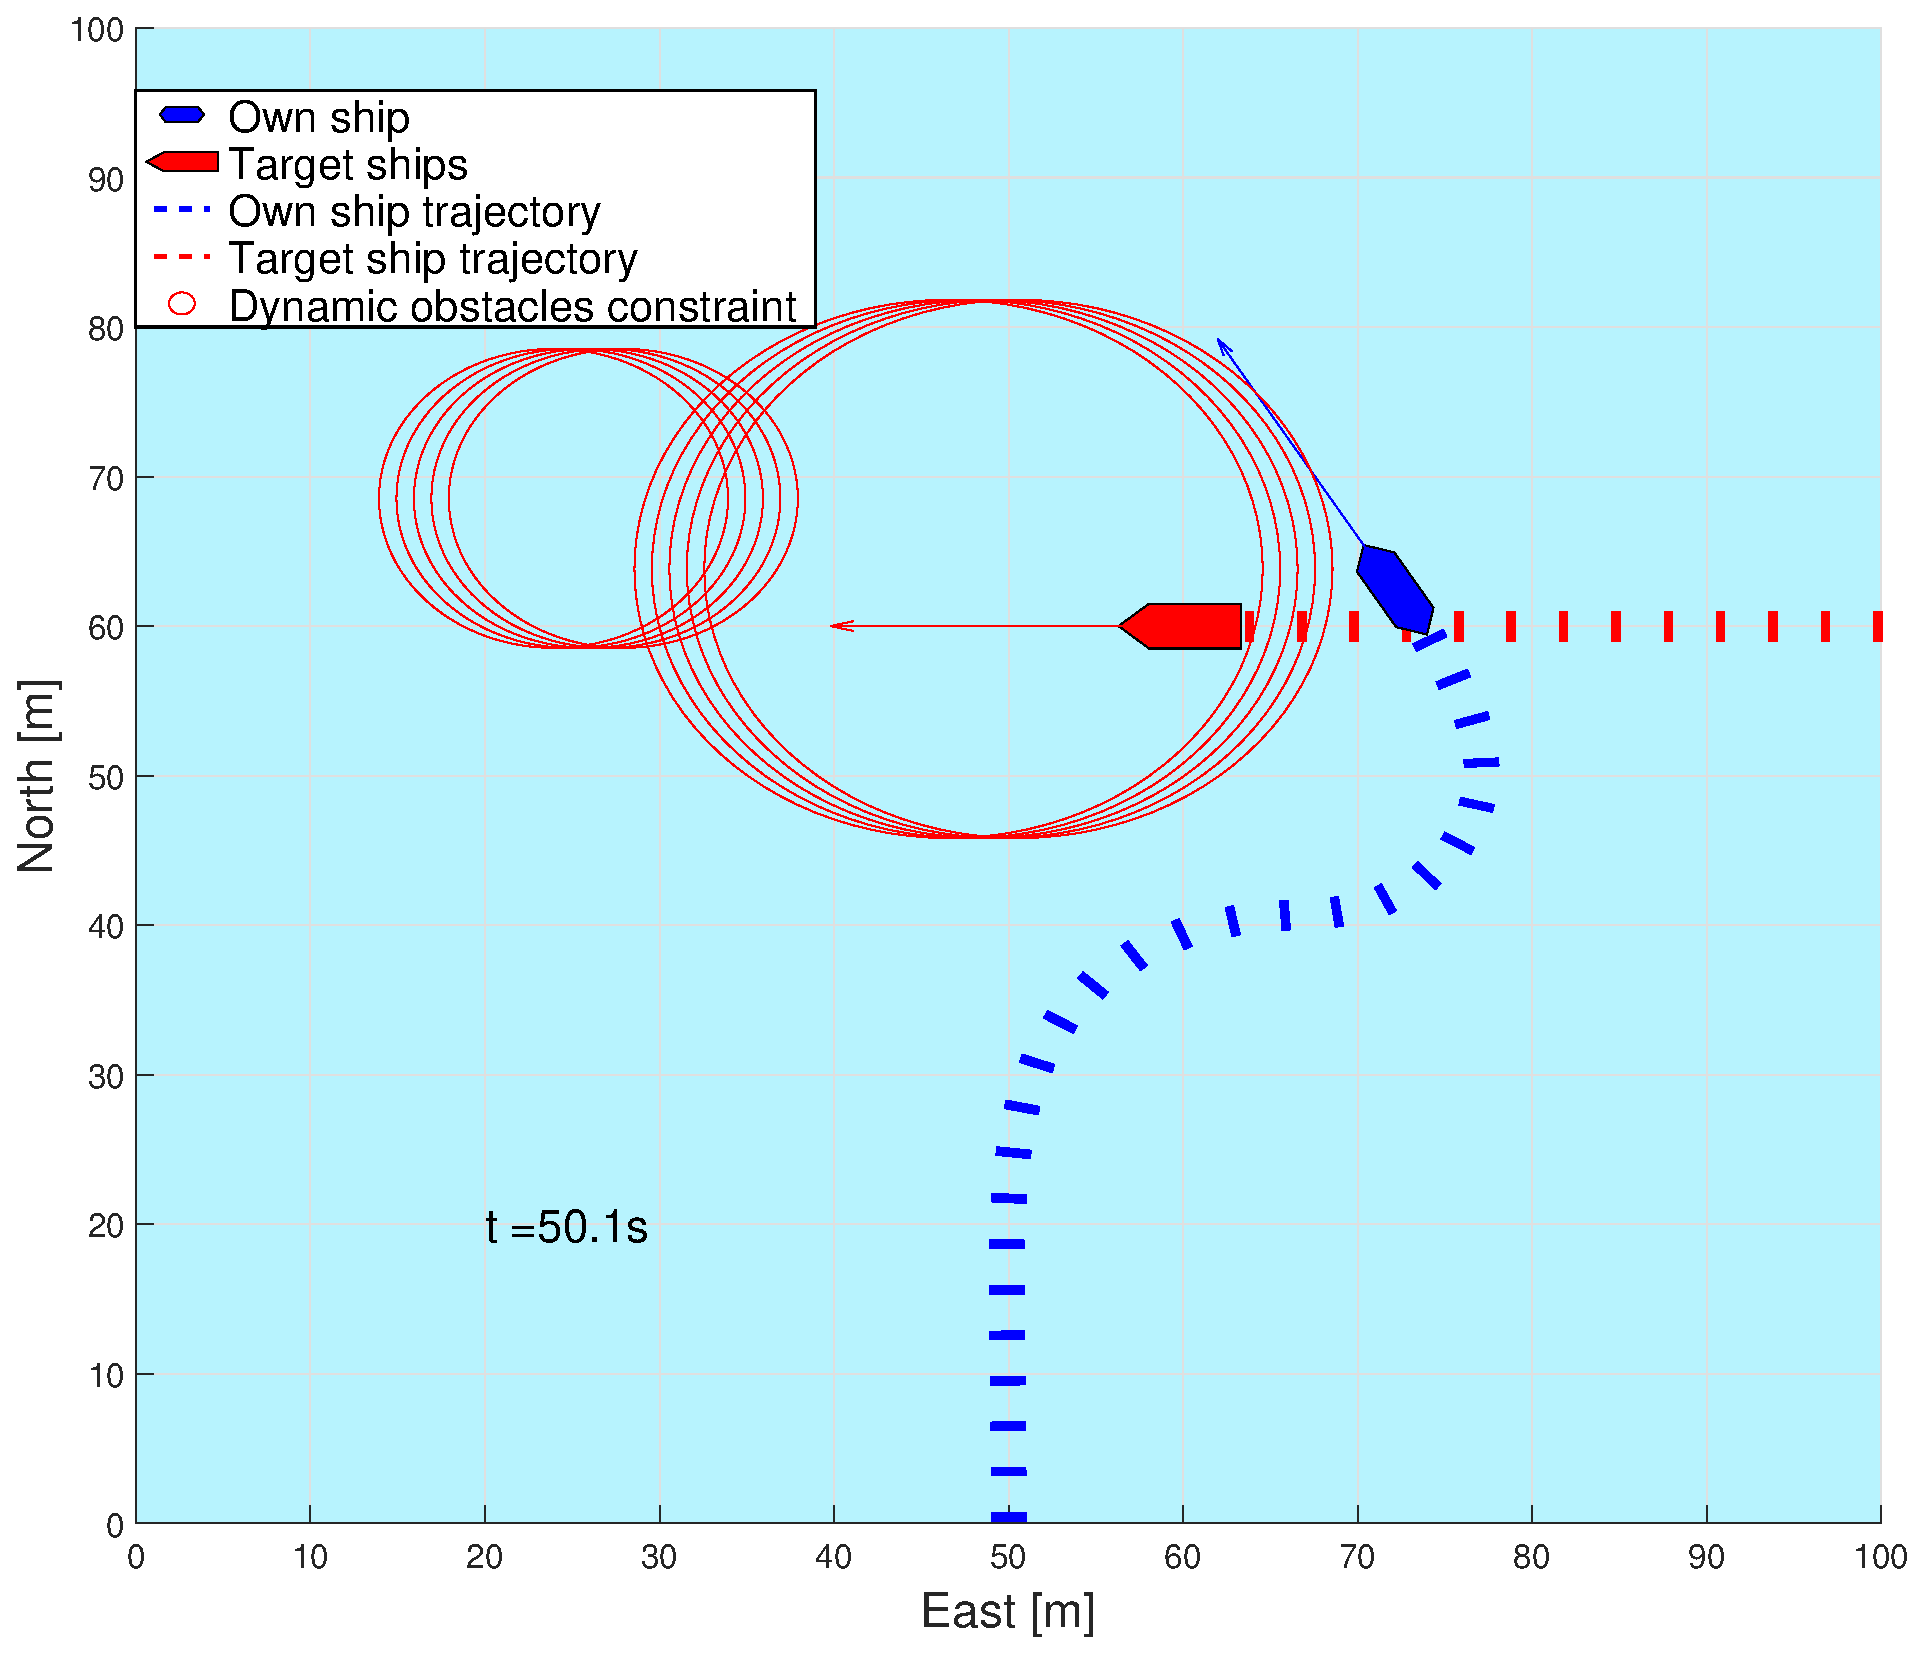
\includegraphics[width=\textwidth]{Images/Figures/enkel_GW/_Simple_0fig1_time=50}
        \subcaption{}
    \end{subfigure}
    \hfill
    \begin{subfigure}[b]{0.499\textwidth}
        \centering
        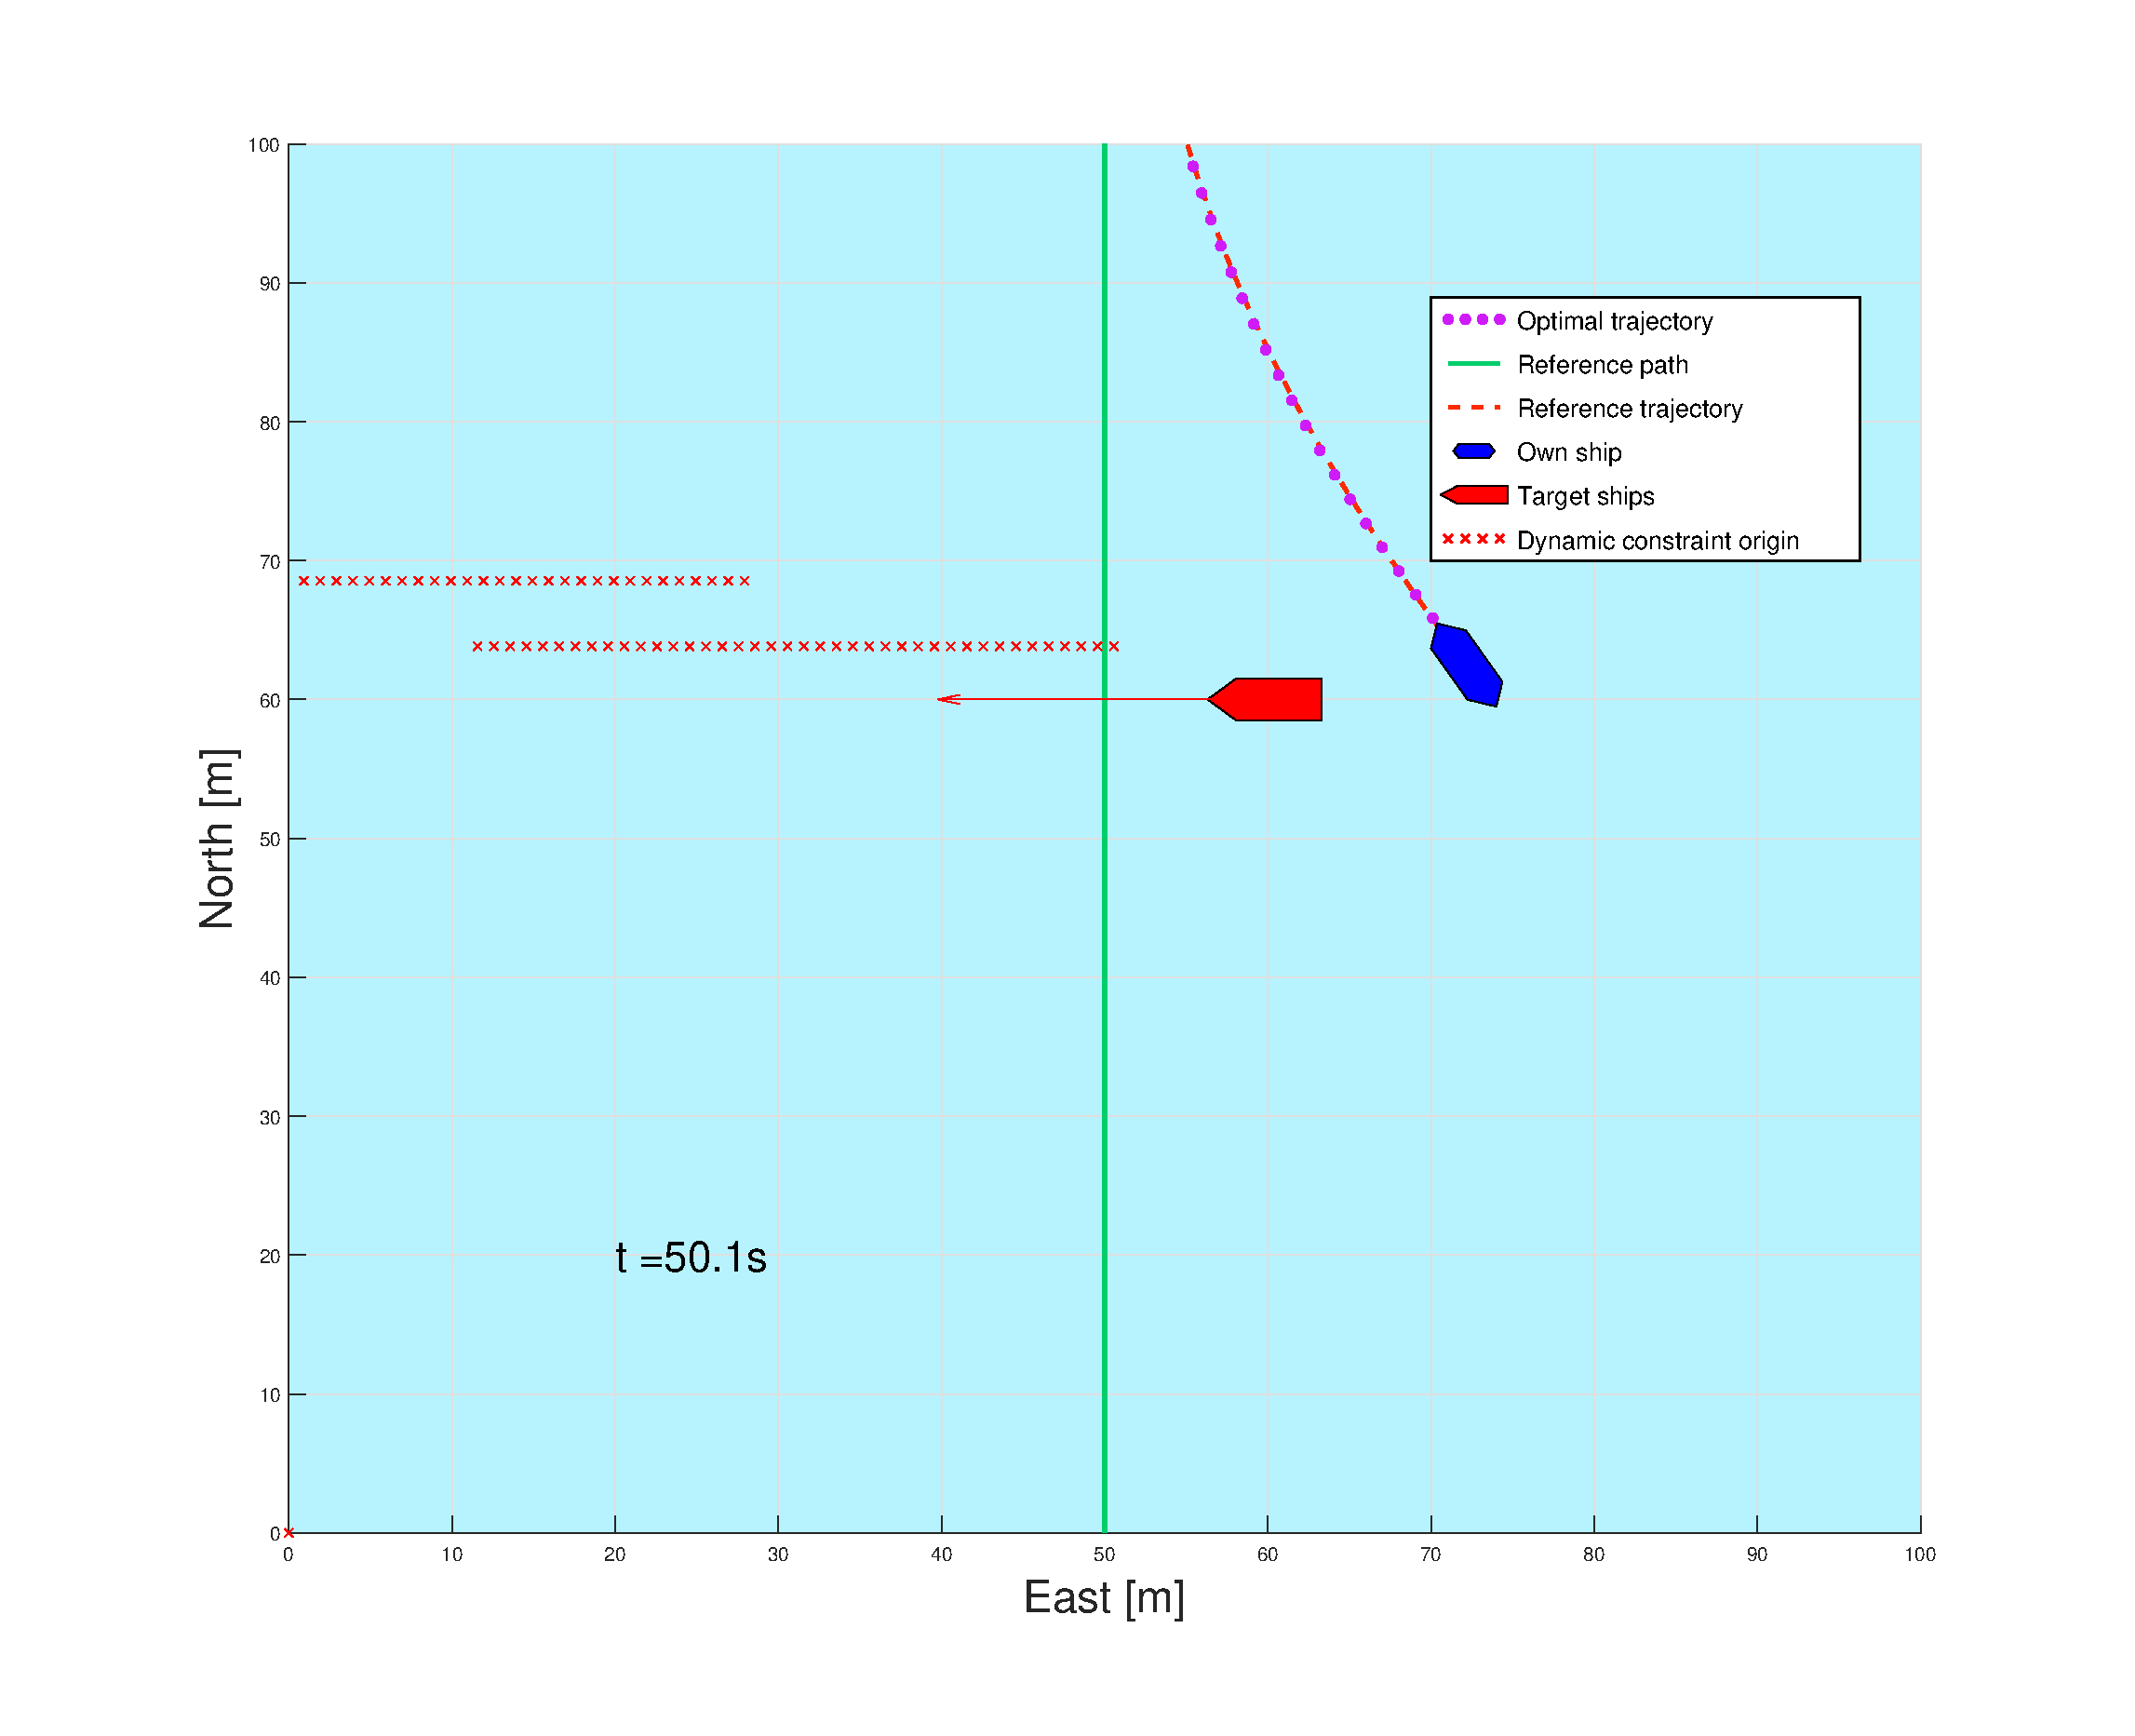
\includegraphics[width=\textwidth]{Images/Figures/enkel_GW/_Simple_0fig999_time=50}
        \subcaption{}
    \end{subfigure}
    \hfill
    \caption{Simple Give Way situation. Result independent of prediction level.}
    \label{FIG: simple GW}
\end{figure}%
% \begin{figure}[ht]\ContinuedFloat
%     \begin{subfigure}[b]{0.49\textwidth}
%         \centering
%         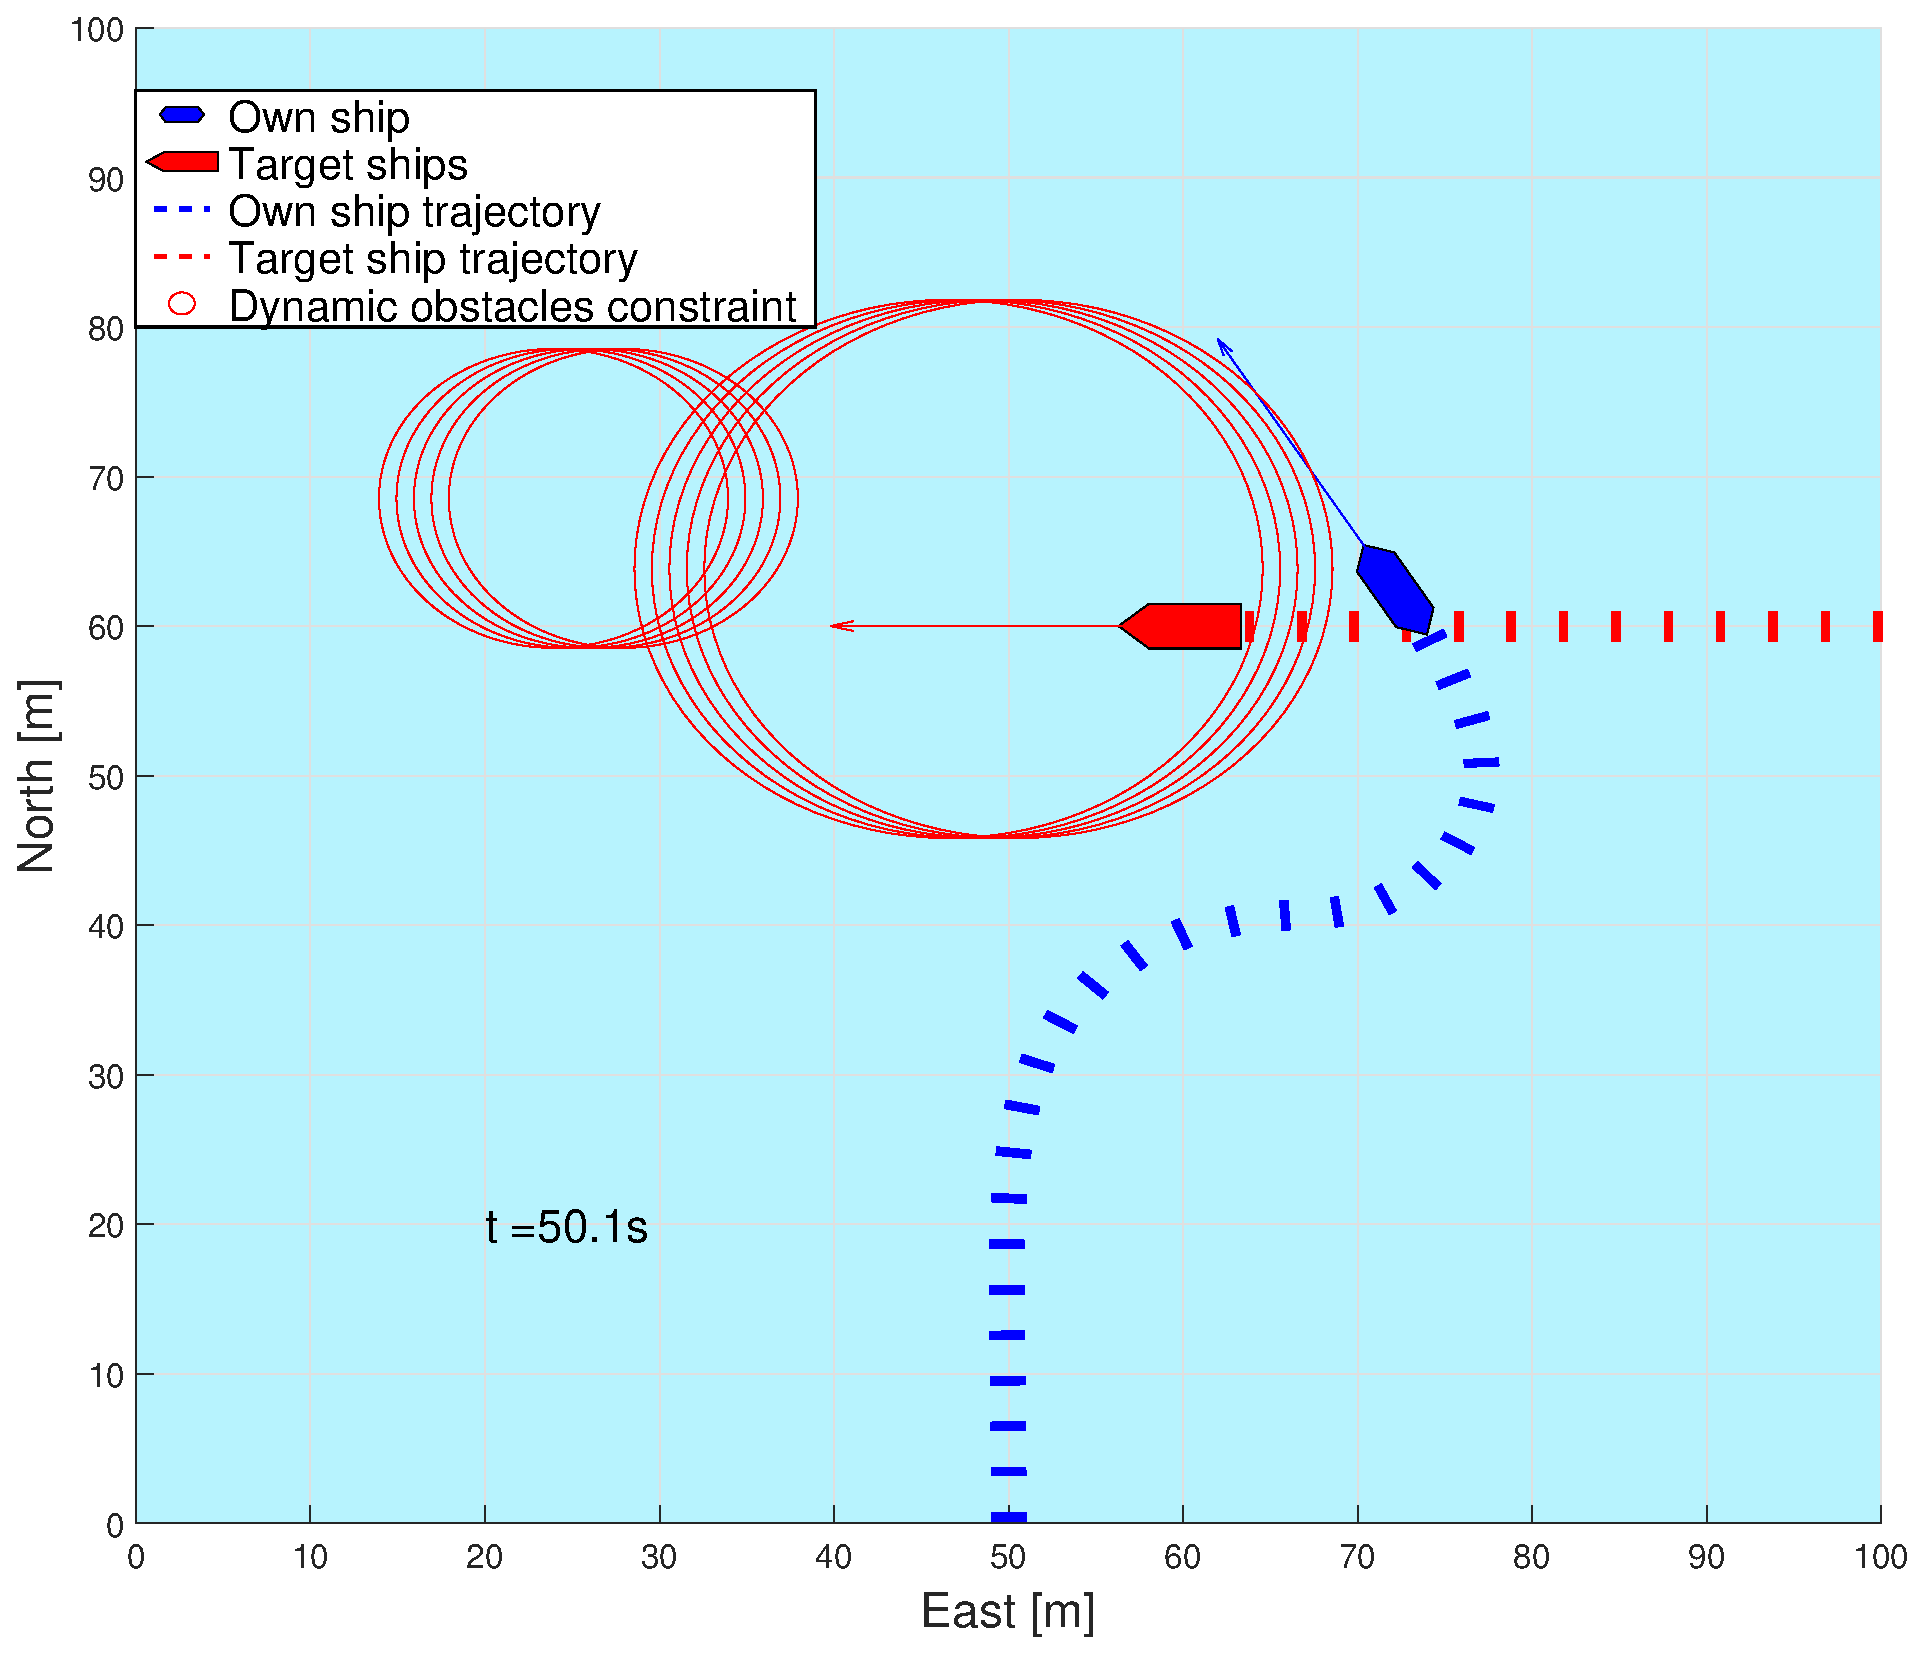
\includegraphics[width=\textwidth]{Images/Figures/enkel_GW/_Simple_0fig1_time=50}
%         \subcaption{}
%     \end{subfigure}
%     \hfill
%     \begin{subfigure}[b]{0.499\textwidth}
%         \centering
%         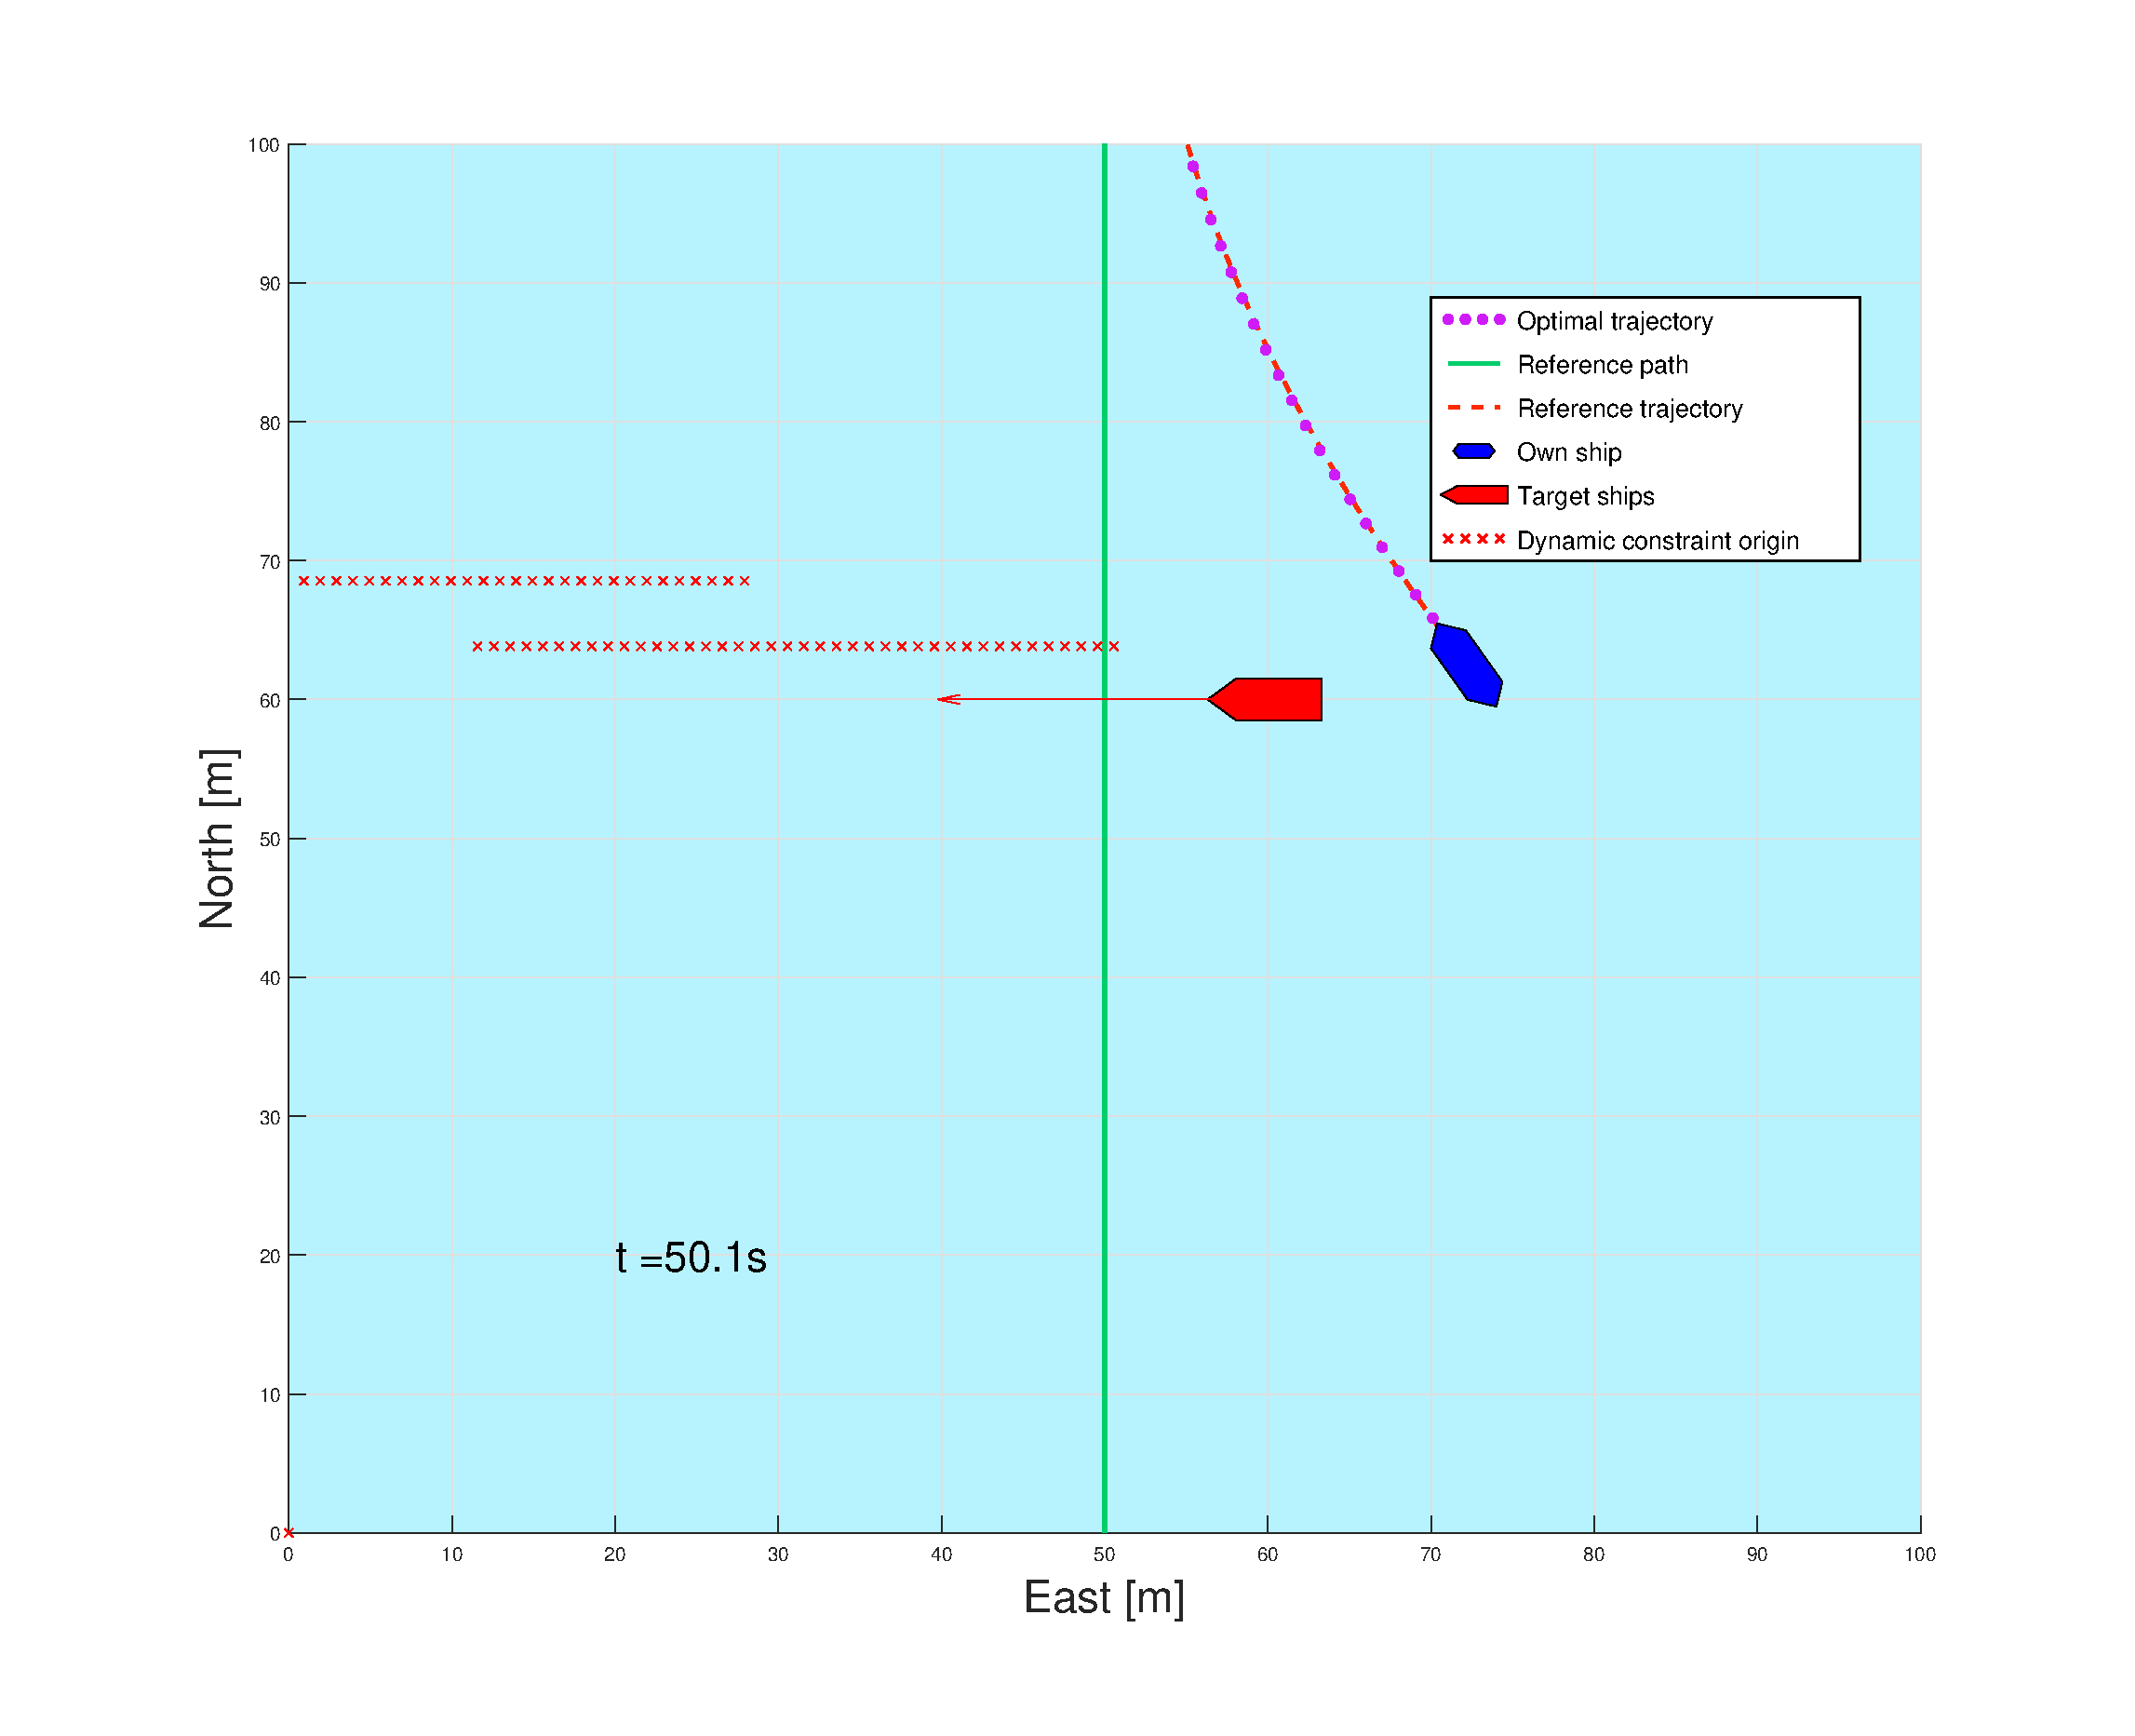
\includegraphics[width=\textwidth]{Images/Figures/enkel_GW/_Simple_0fig999_time=50}
%         \subcaption{}
%     \end{subfigure}
%     \hfill
%     \\
%     \begin{subfigure}[b]{0.49\textwidth}
%         \centering
%         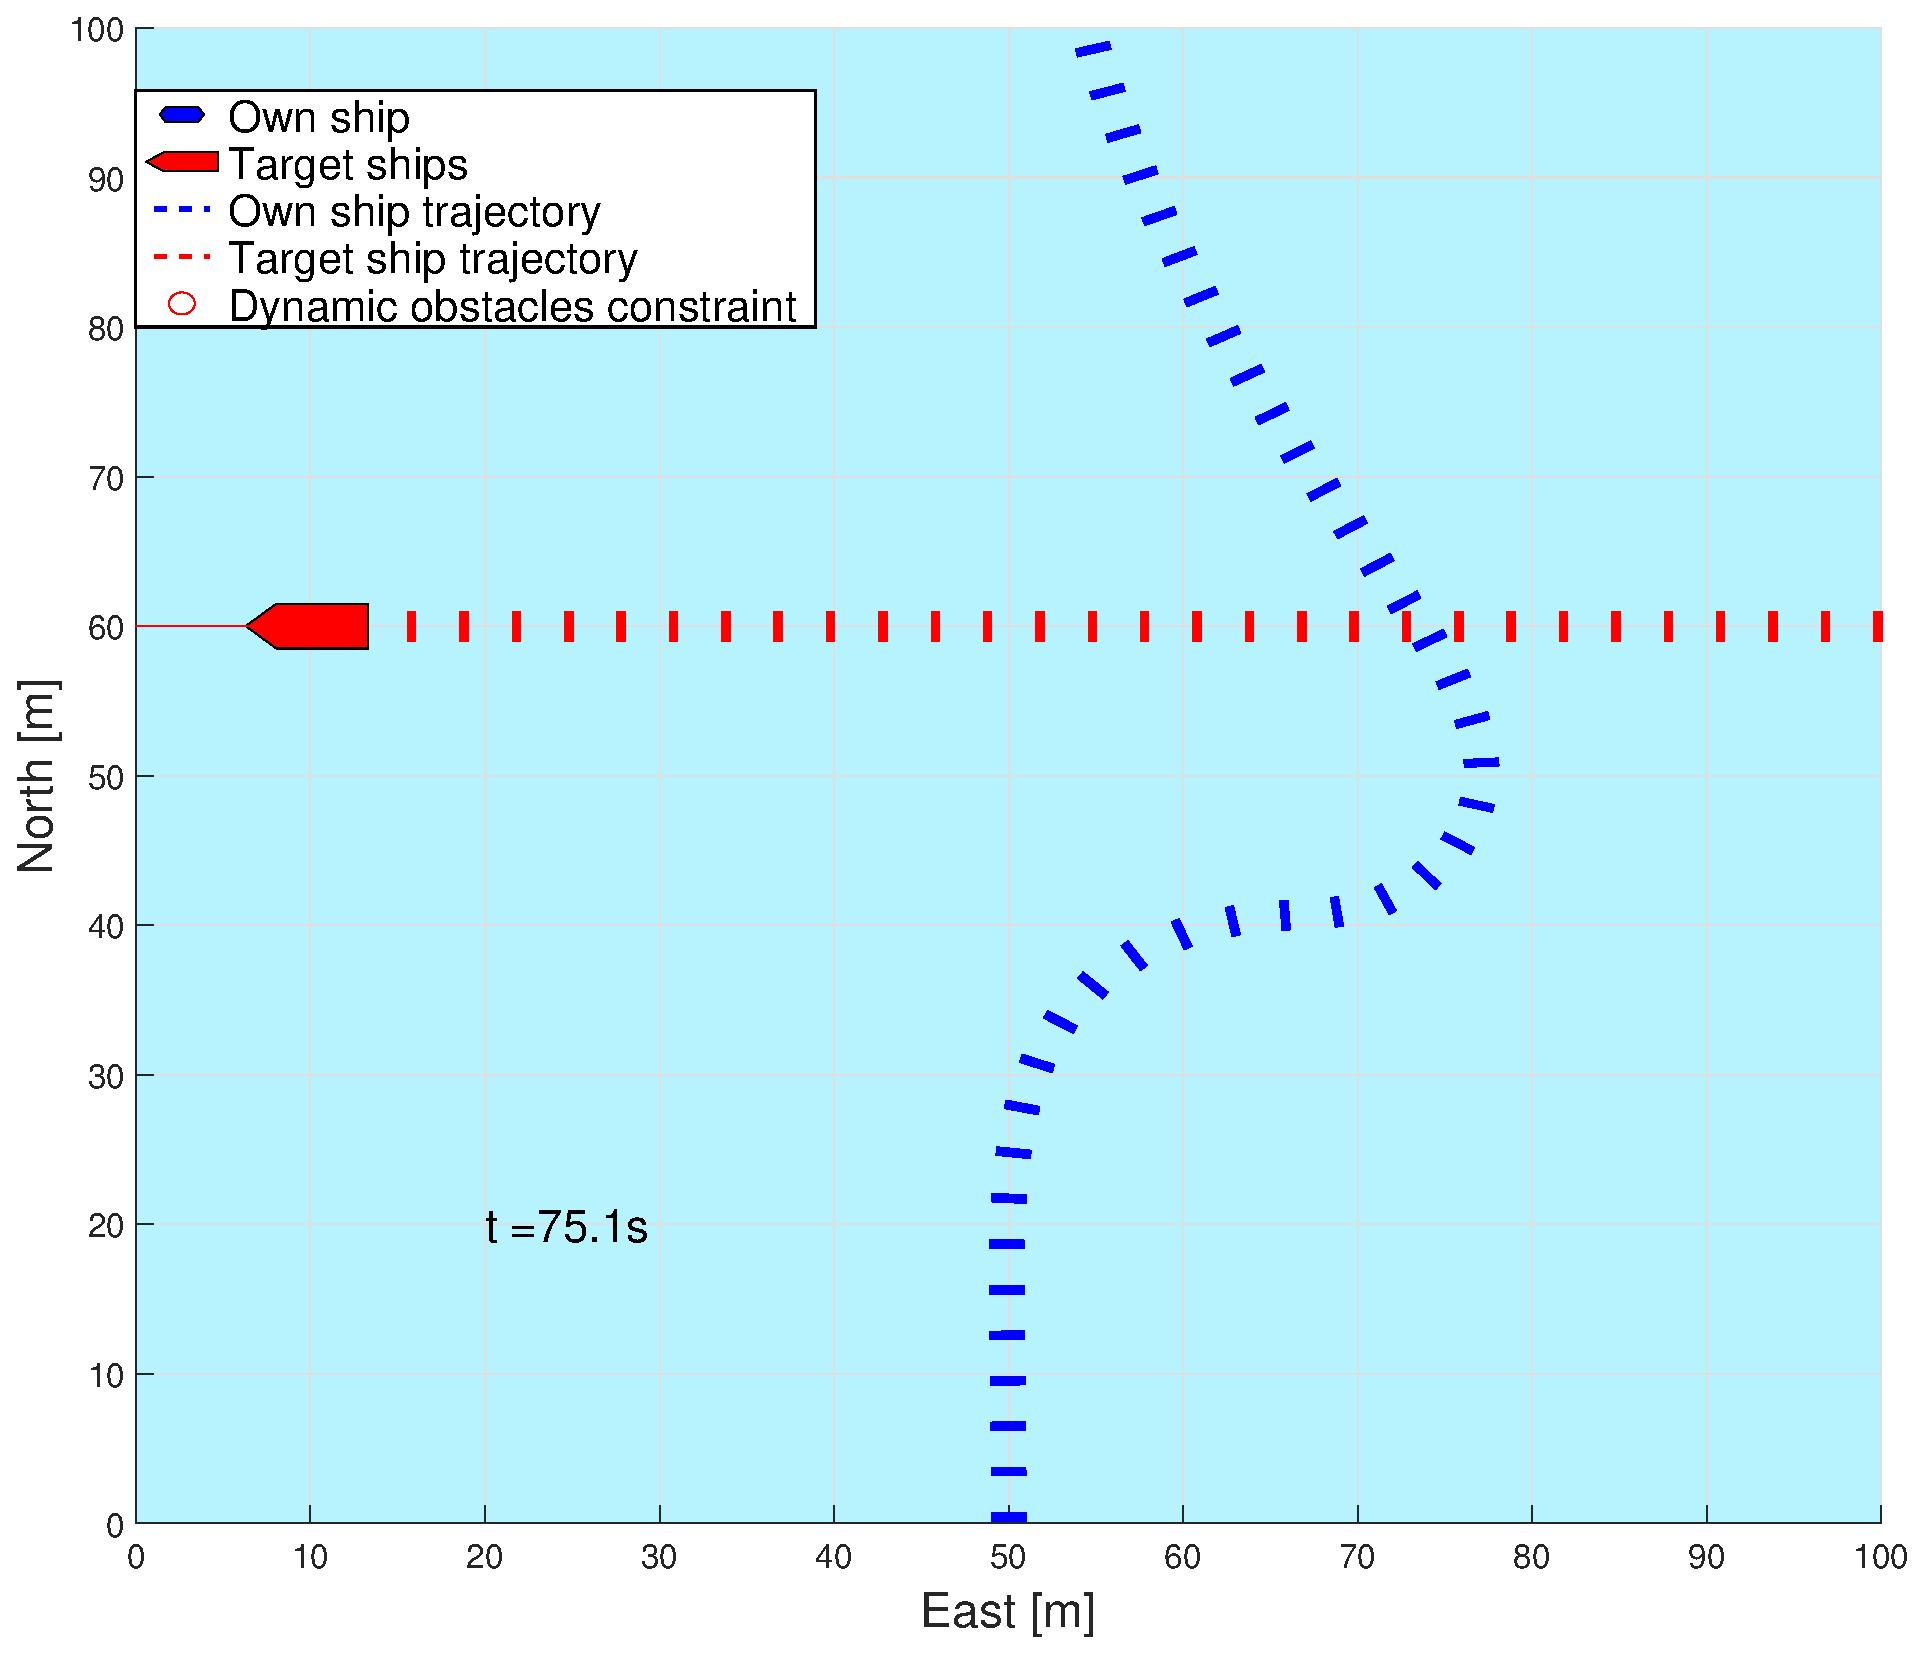
\includegraphics[width=\textwidth]{Images/Figures/enkel_GW/_Simple_0fig1_time=75}
%         \subcaption{}
%     \end{subfigure}
%     \hfill
%     \begin{subfigure}[b]{0.499\textwidth}
%         \centering
%         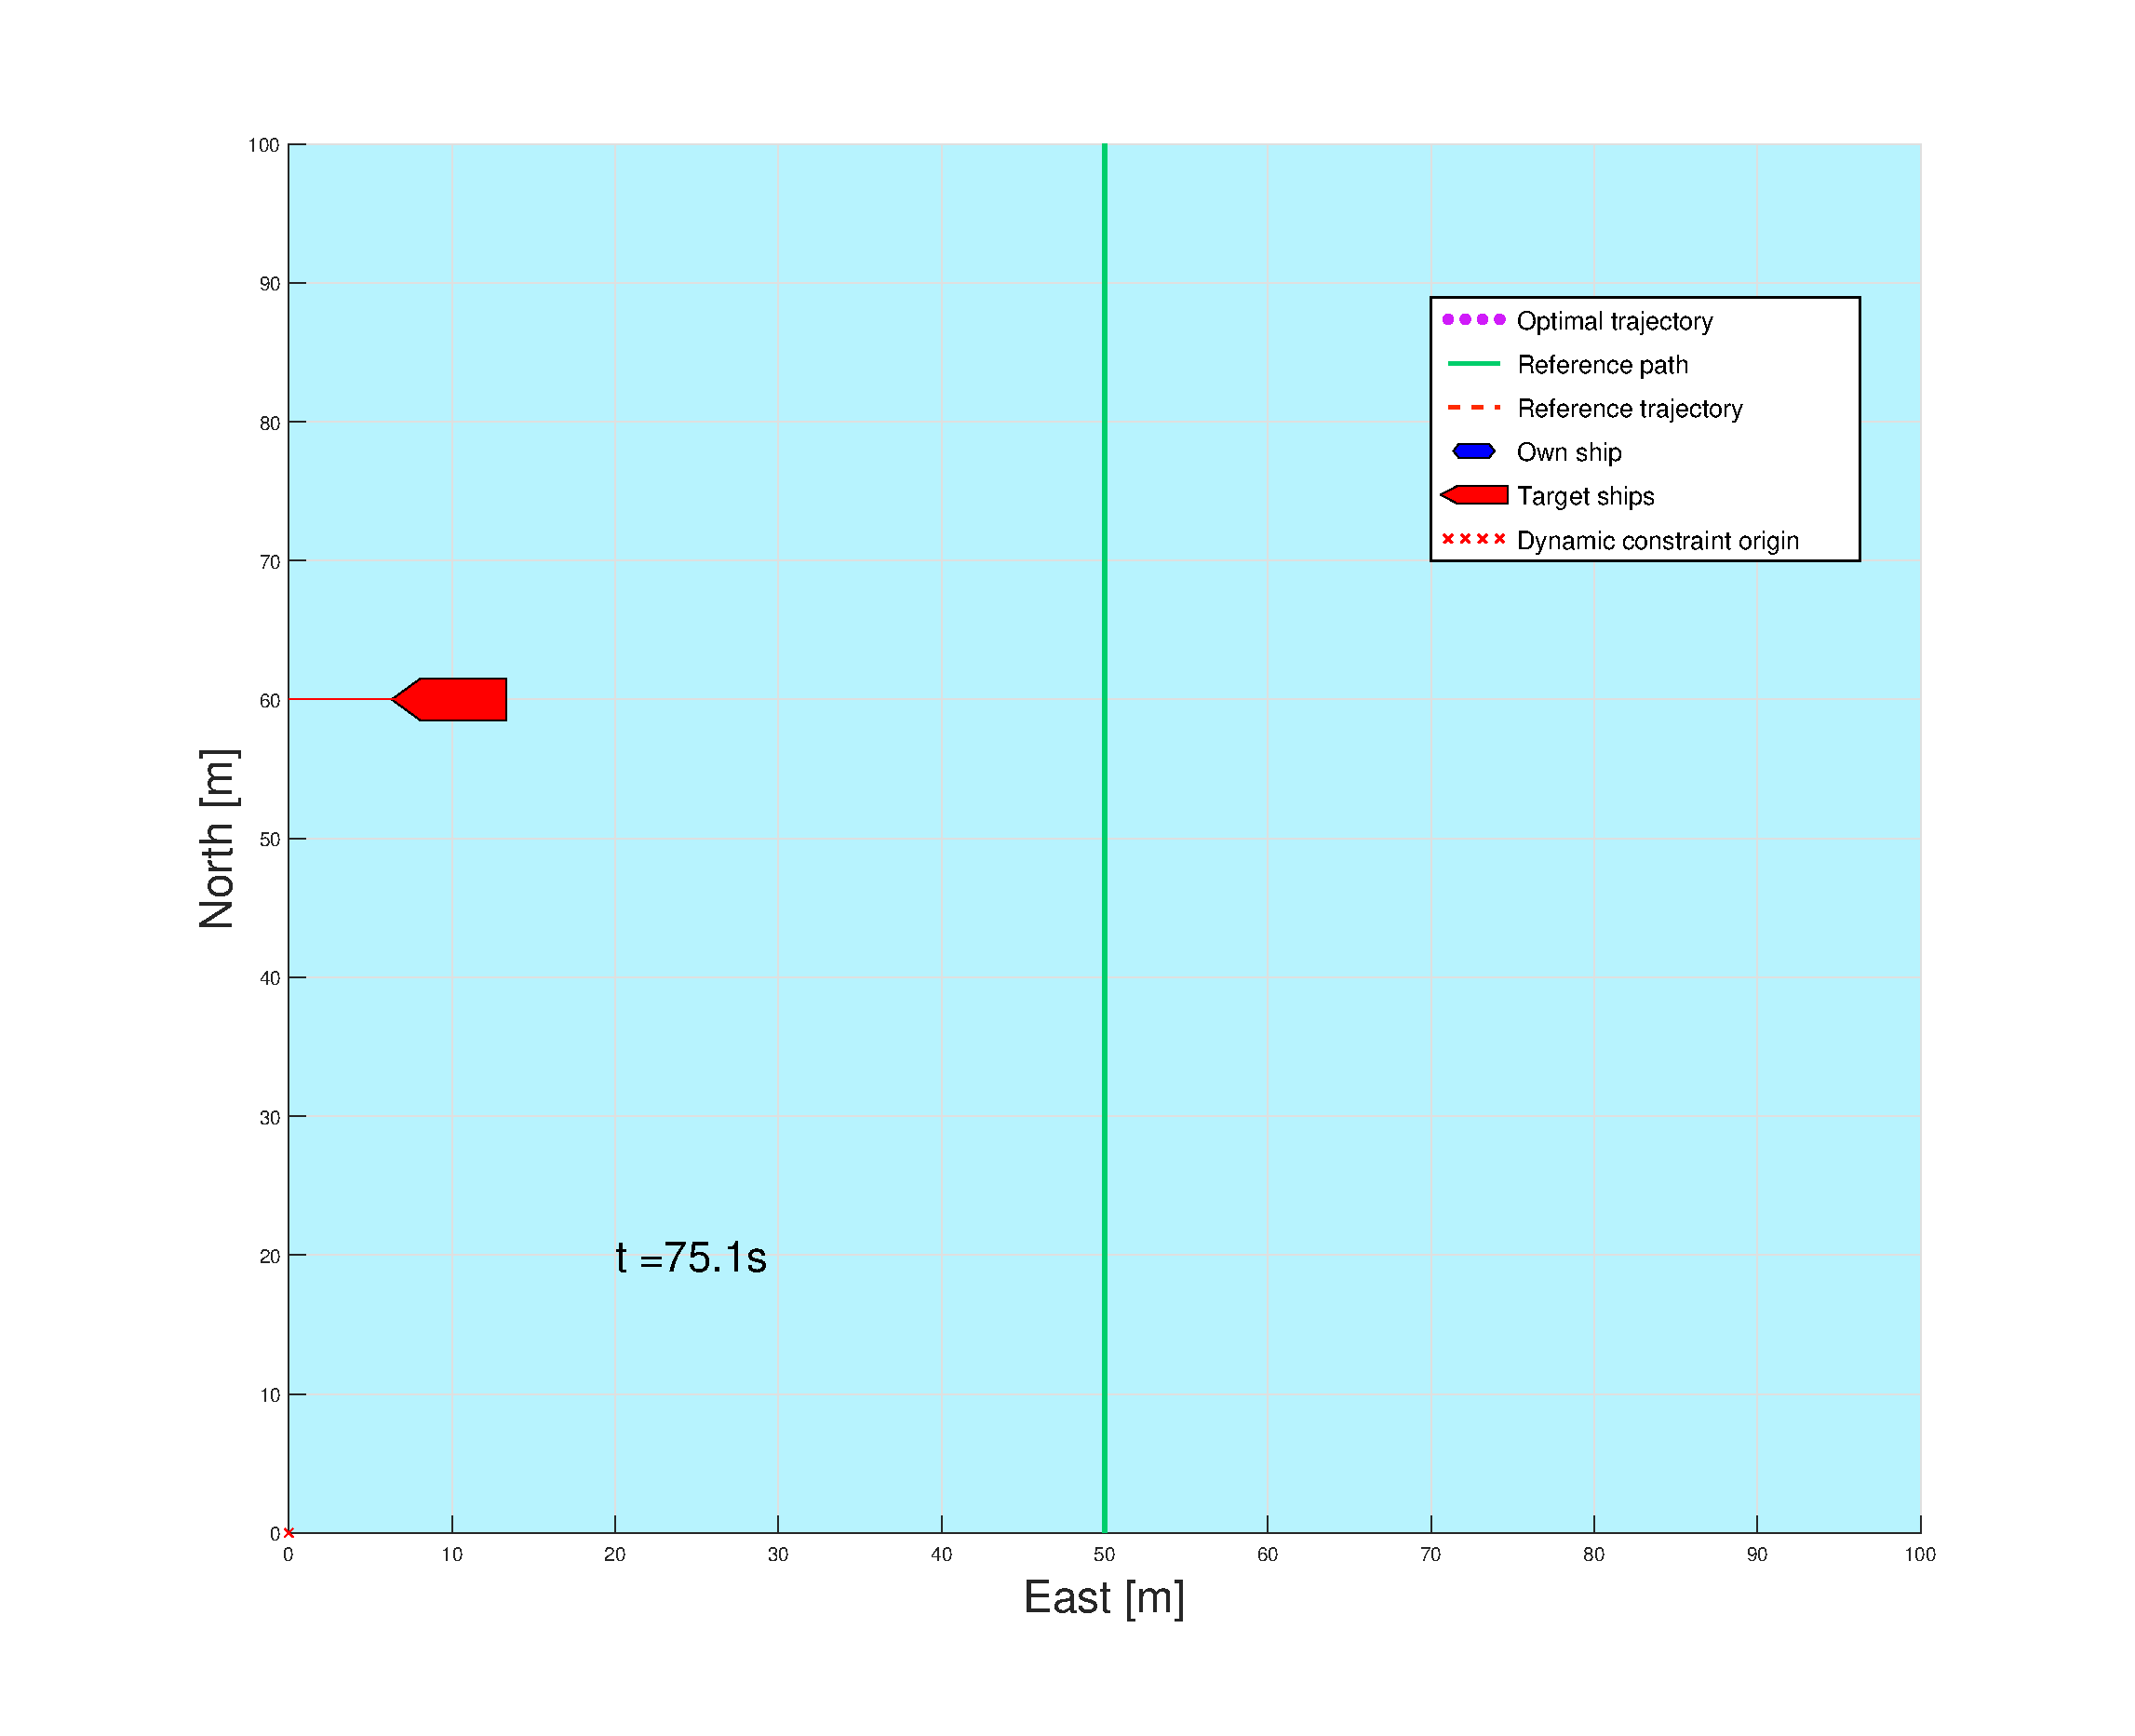
\includegraphics[width=\textwidth]{Images/Figures/enkel_GW/_Simple_0fig999_time=75}
%         \subcaption{}
%     \end{subfigure}
%     \hfill
%     \caption{Simple Give Way With Prediction}
% \end{figure}

% \begin{figure}[!b] 
%     \begin{subfigure}[b]{0.49\textwidth}
%         \centering
%         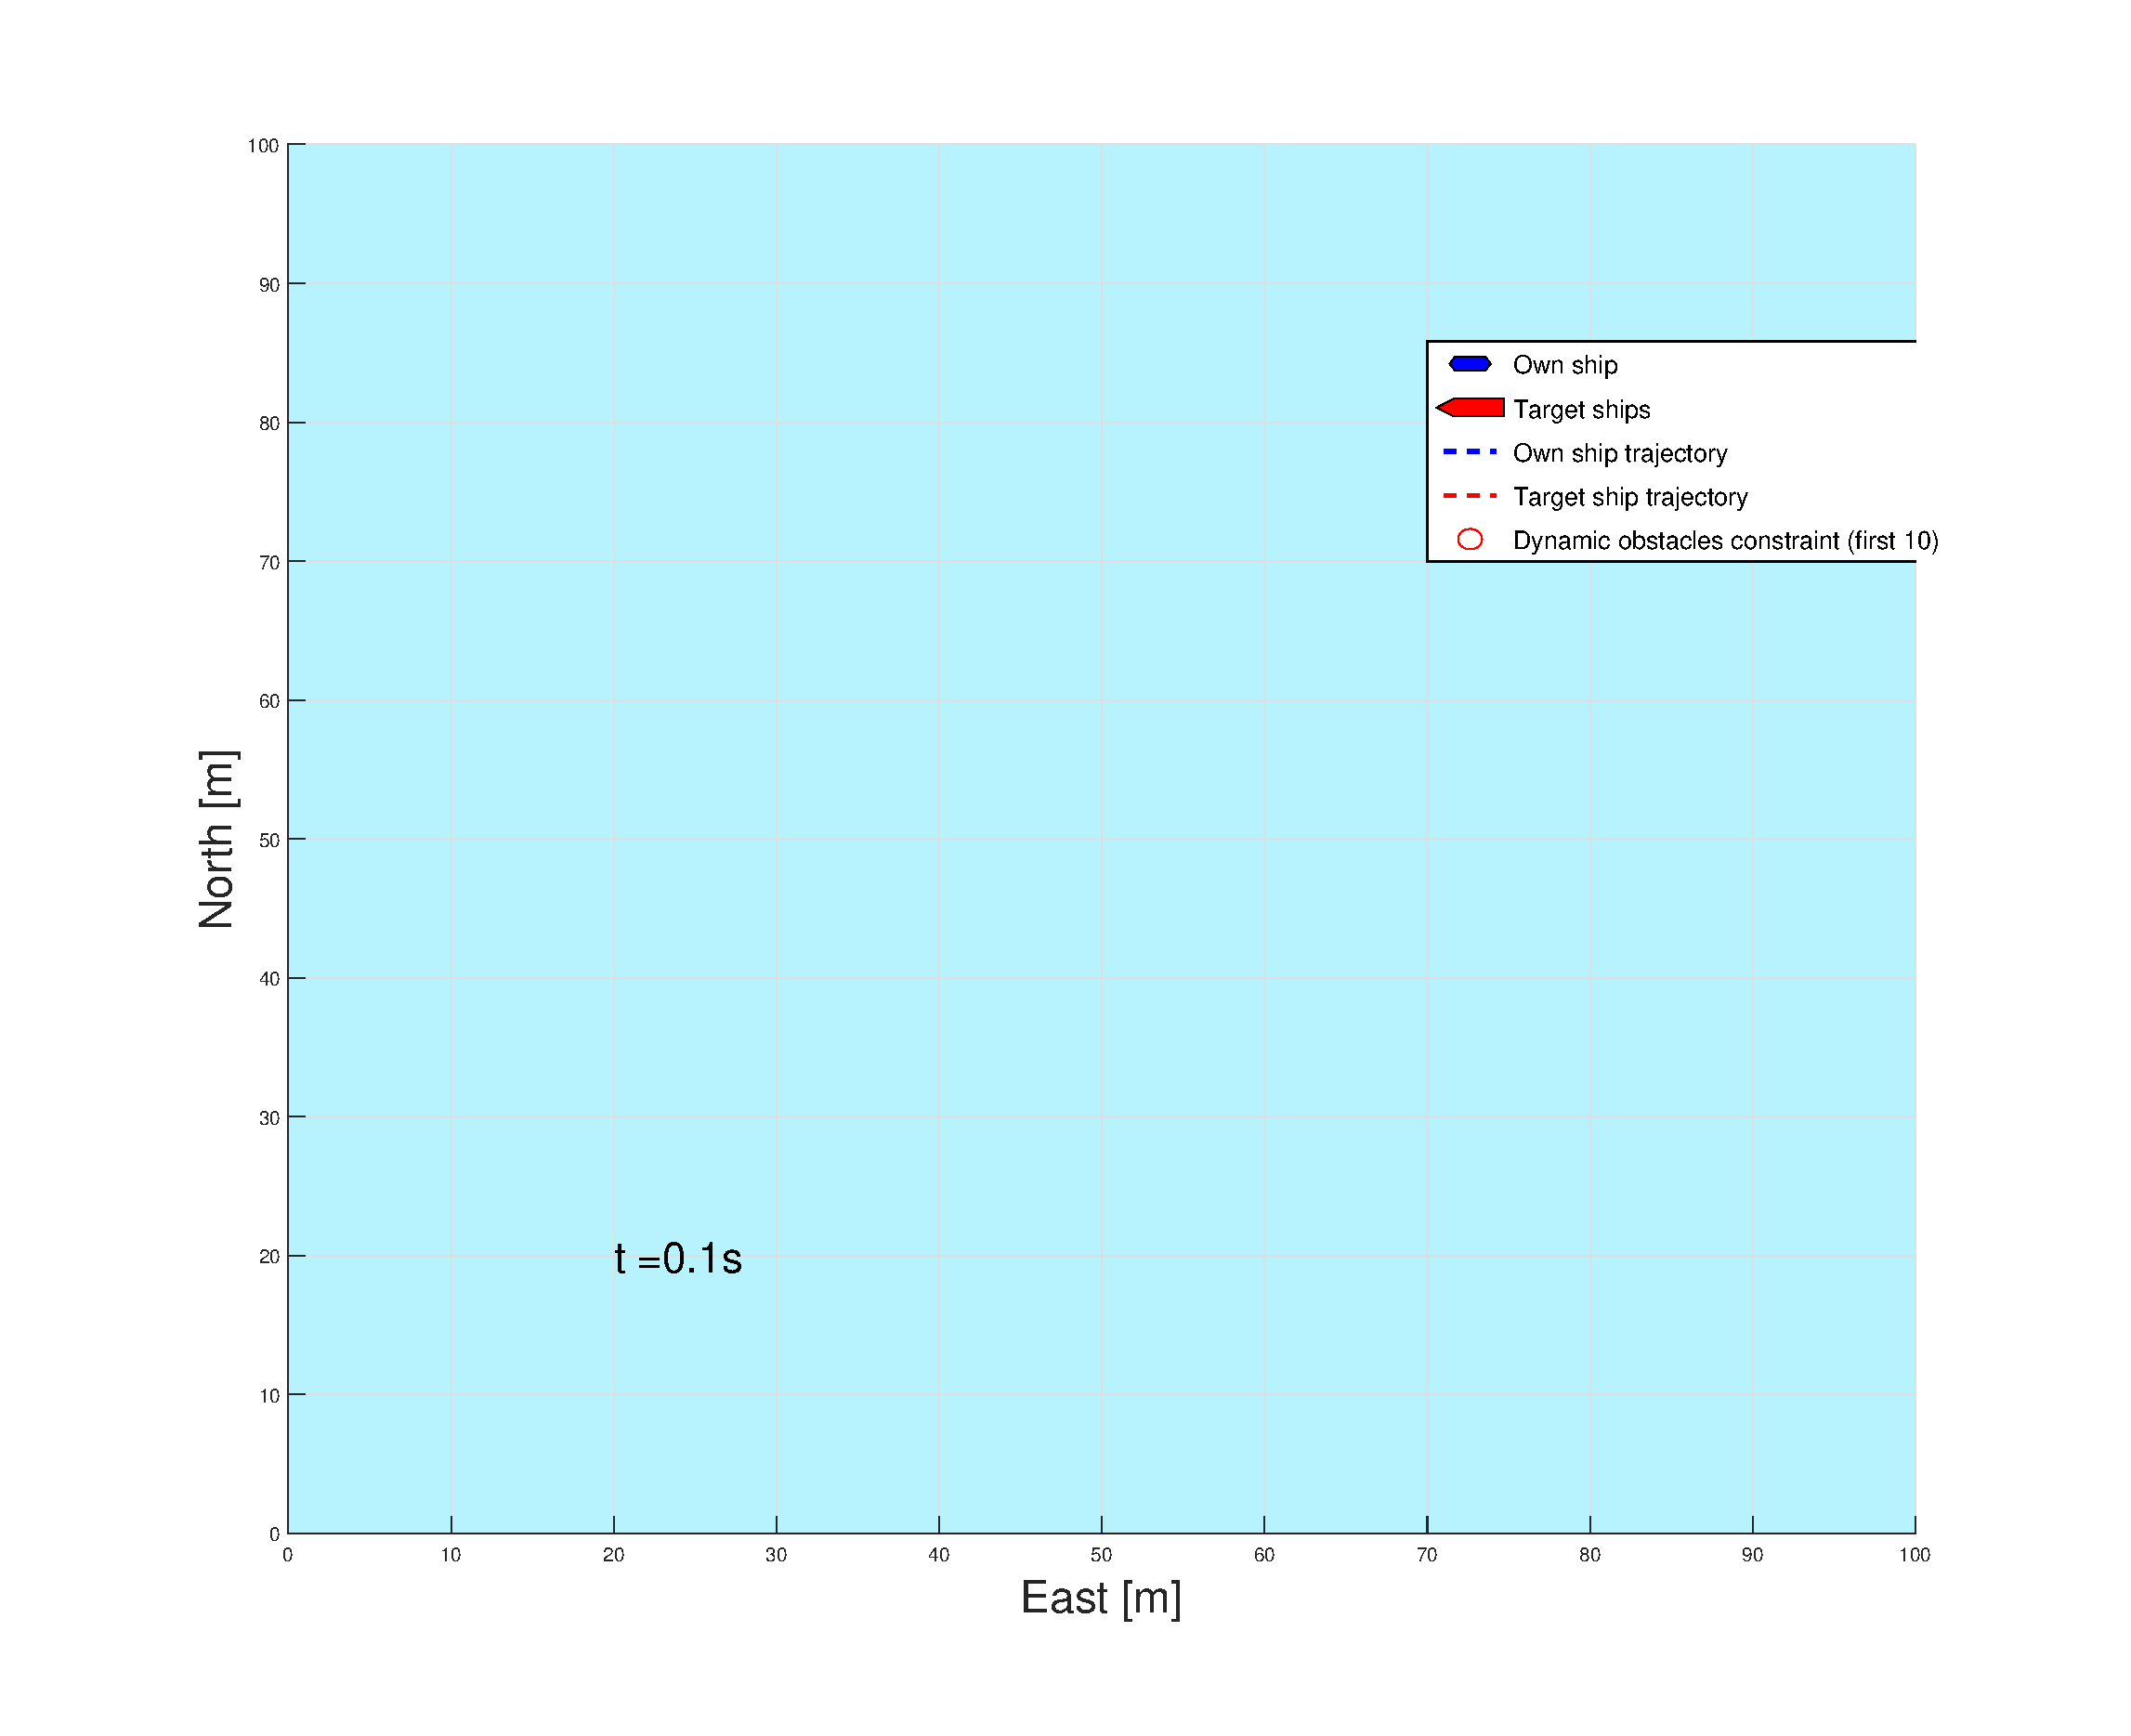
\includegraphics[width=\textwidth]{Images/Figures/enkel_GW/_Simple_1fig1_time=0}
%         \subcaption{}
%     \end{subfigure}
%     \hfill
%     \begin{subfigure}[b]{0.499\textwidth}
%         \centering
%         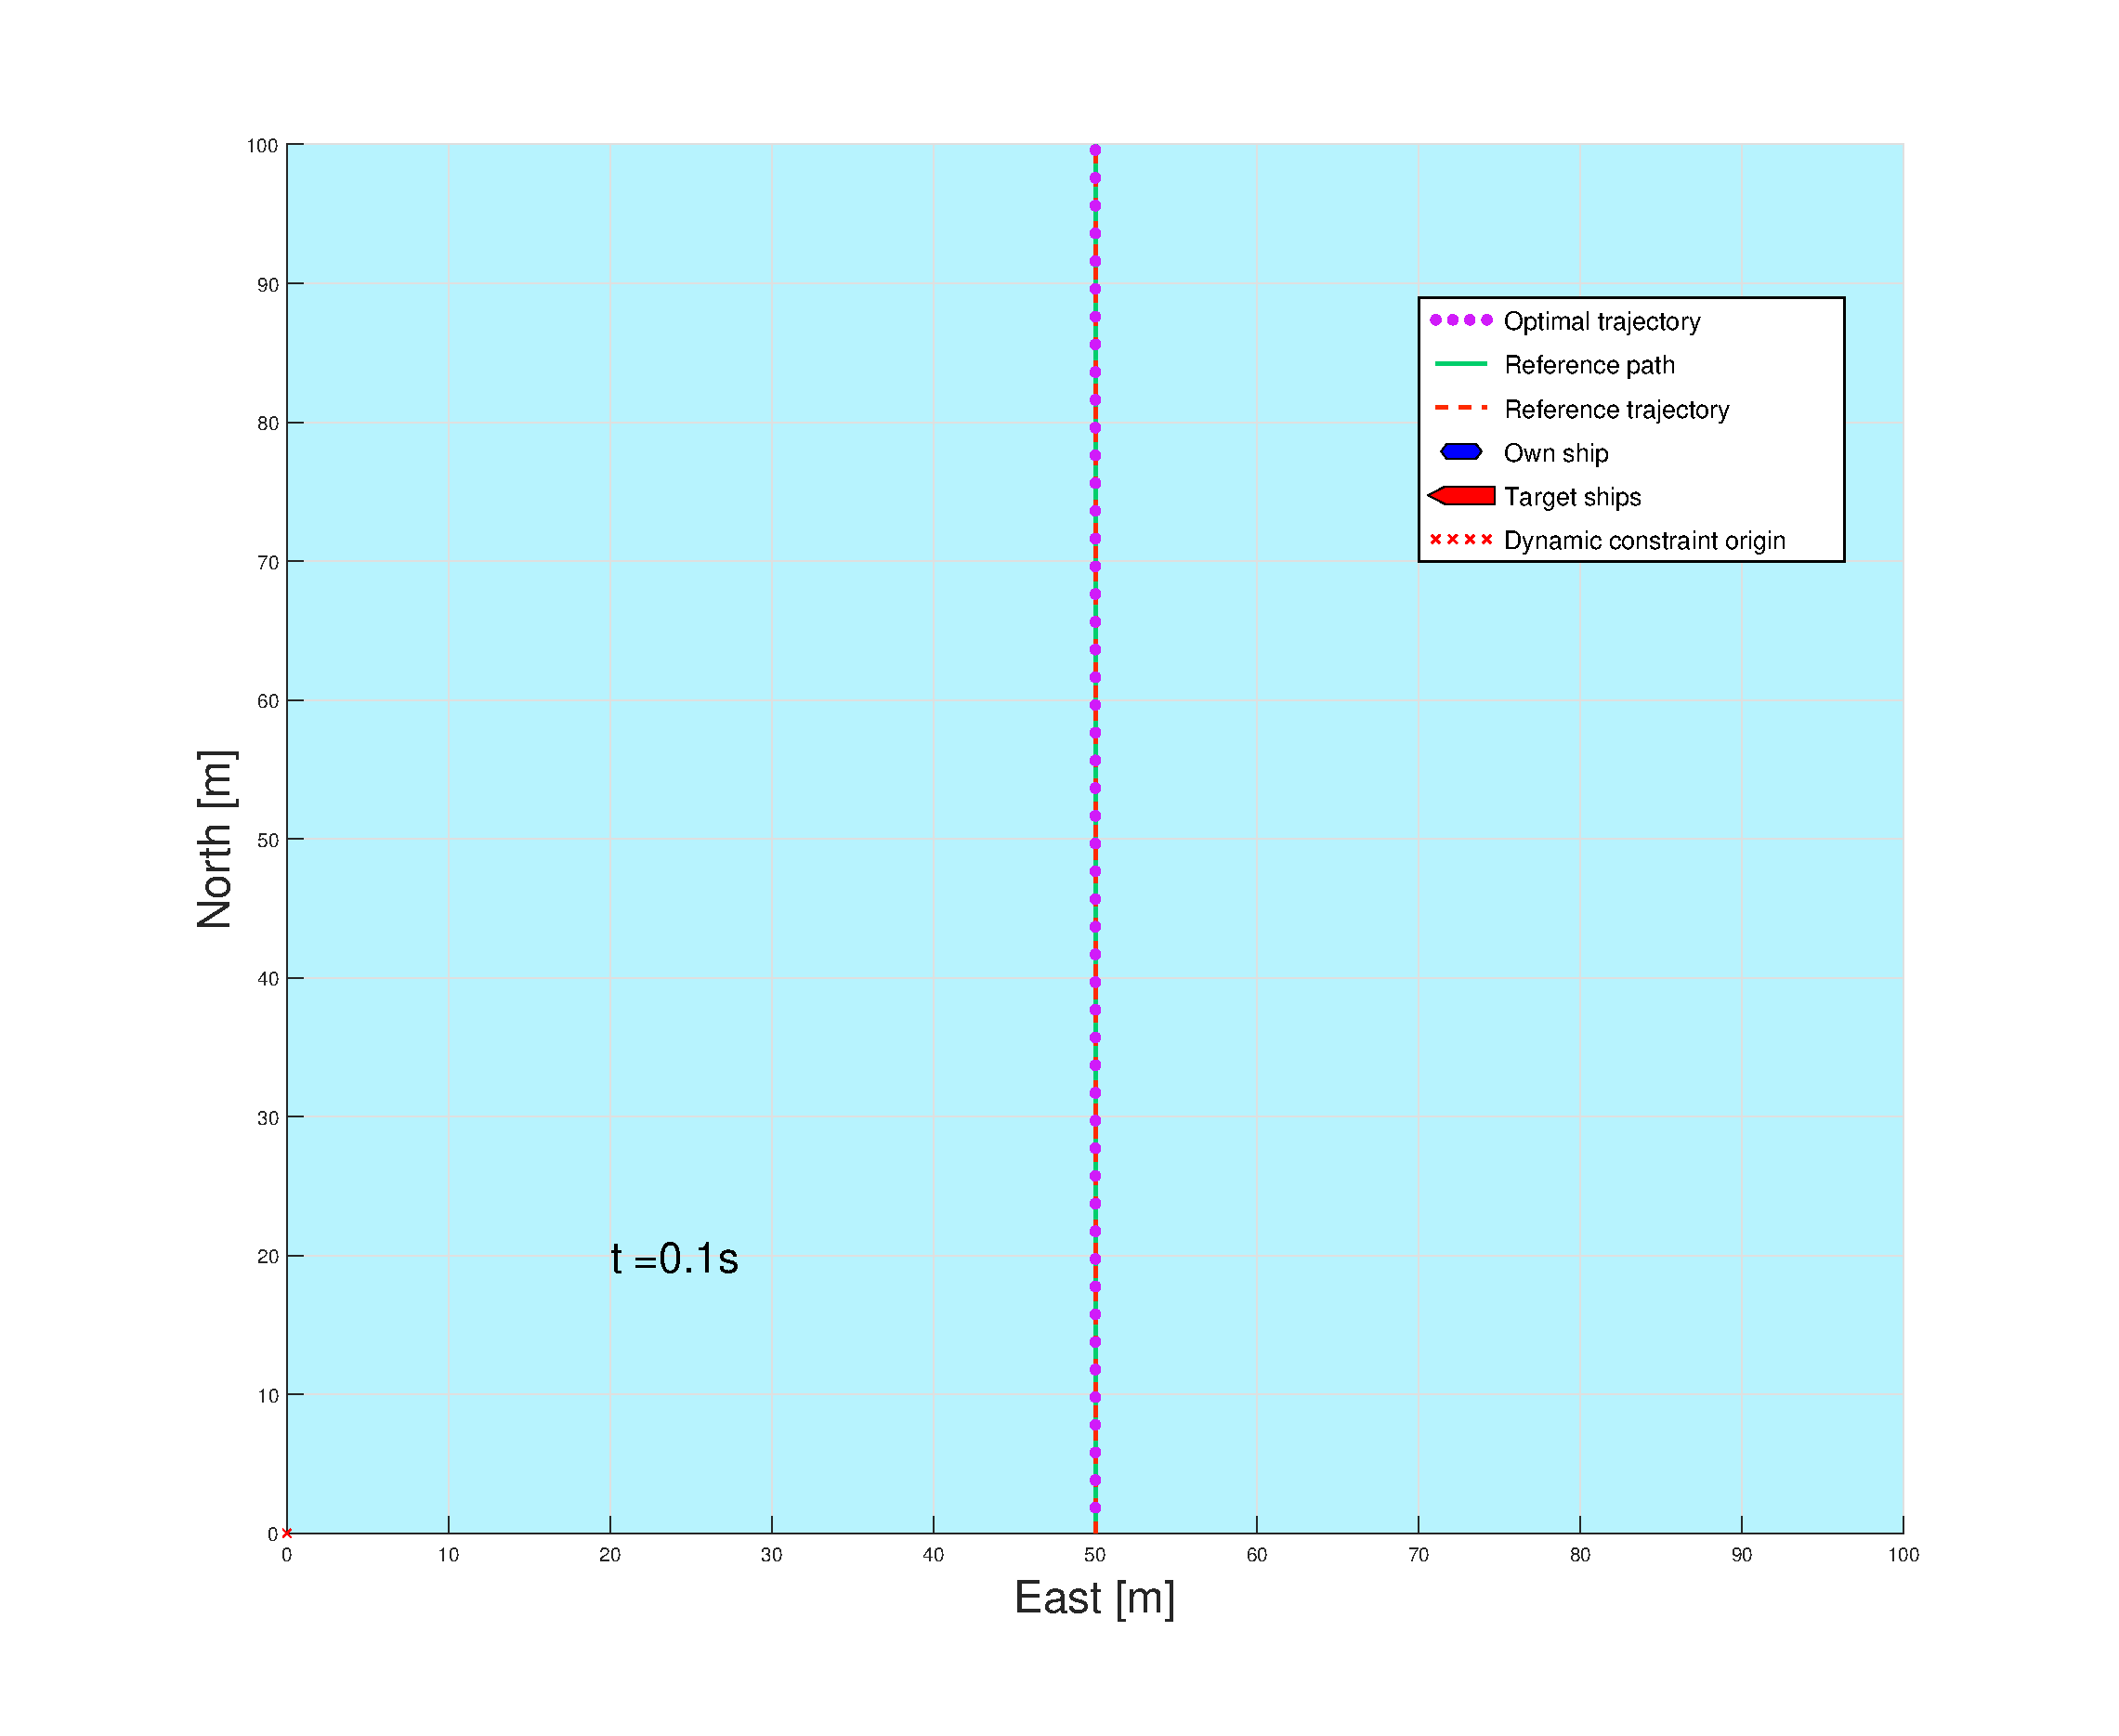
\includegraphics[width=\textwidth]{Images/Figures/enkel_GW/_Simple_1fig999_time=0}
%         \subcaption{}
%     \end{subfigure}
%     \hfill
%     \\
%     \begin{subfigure}[b]{0.49\textwidth}
%         \centering
%         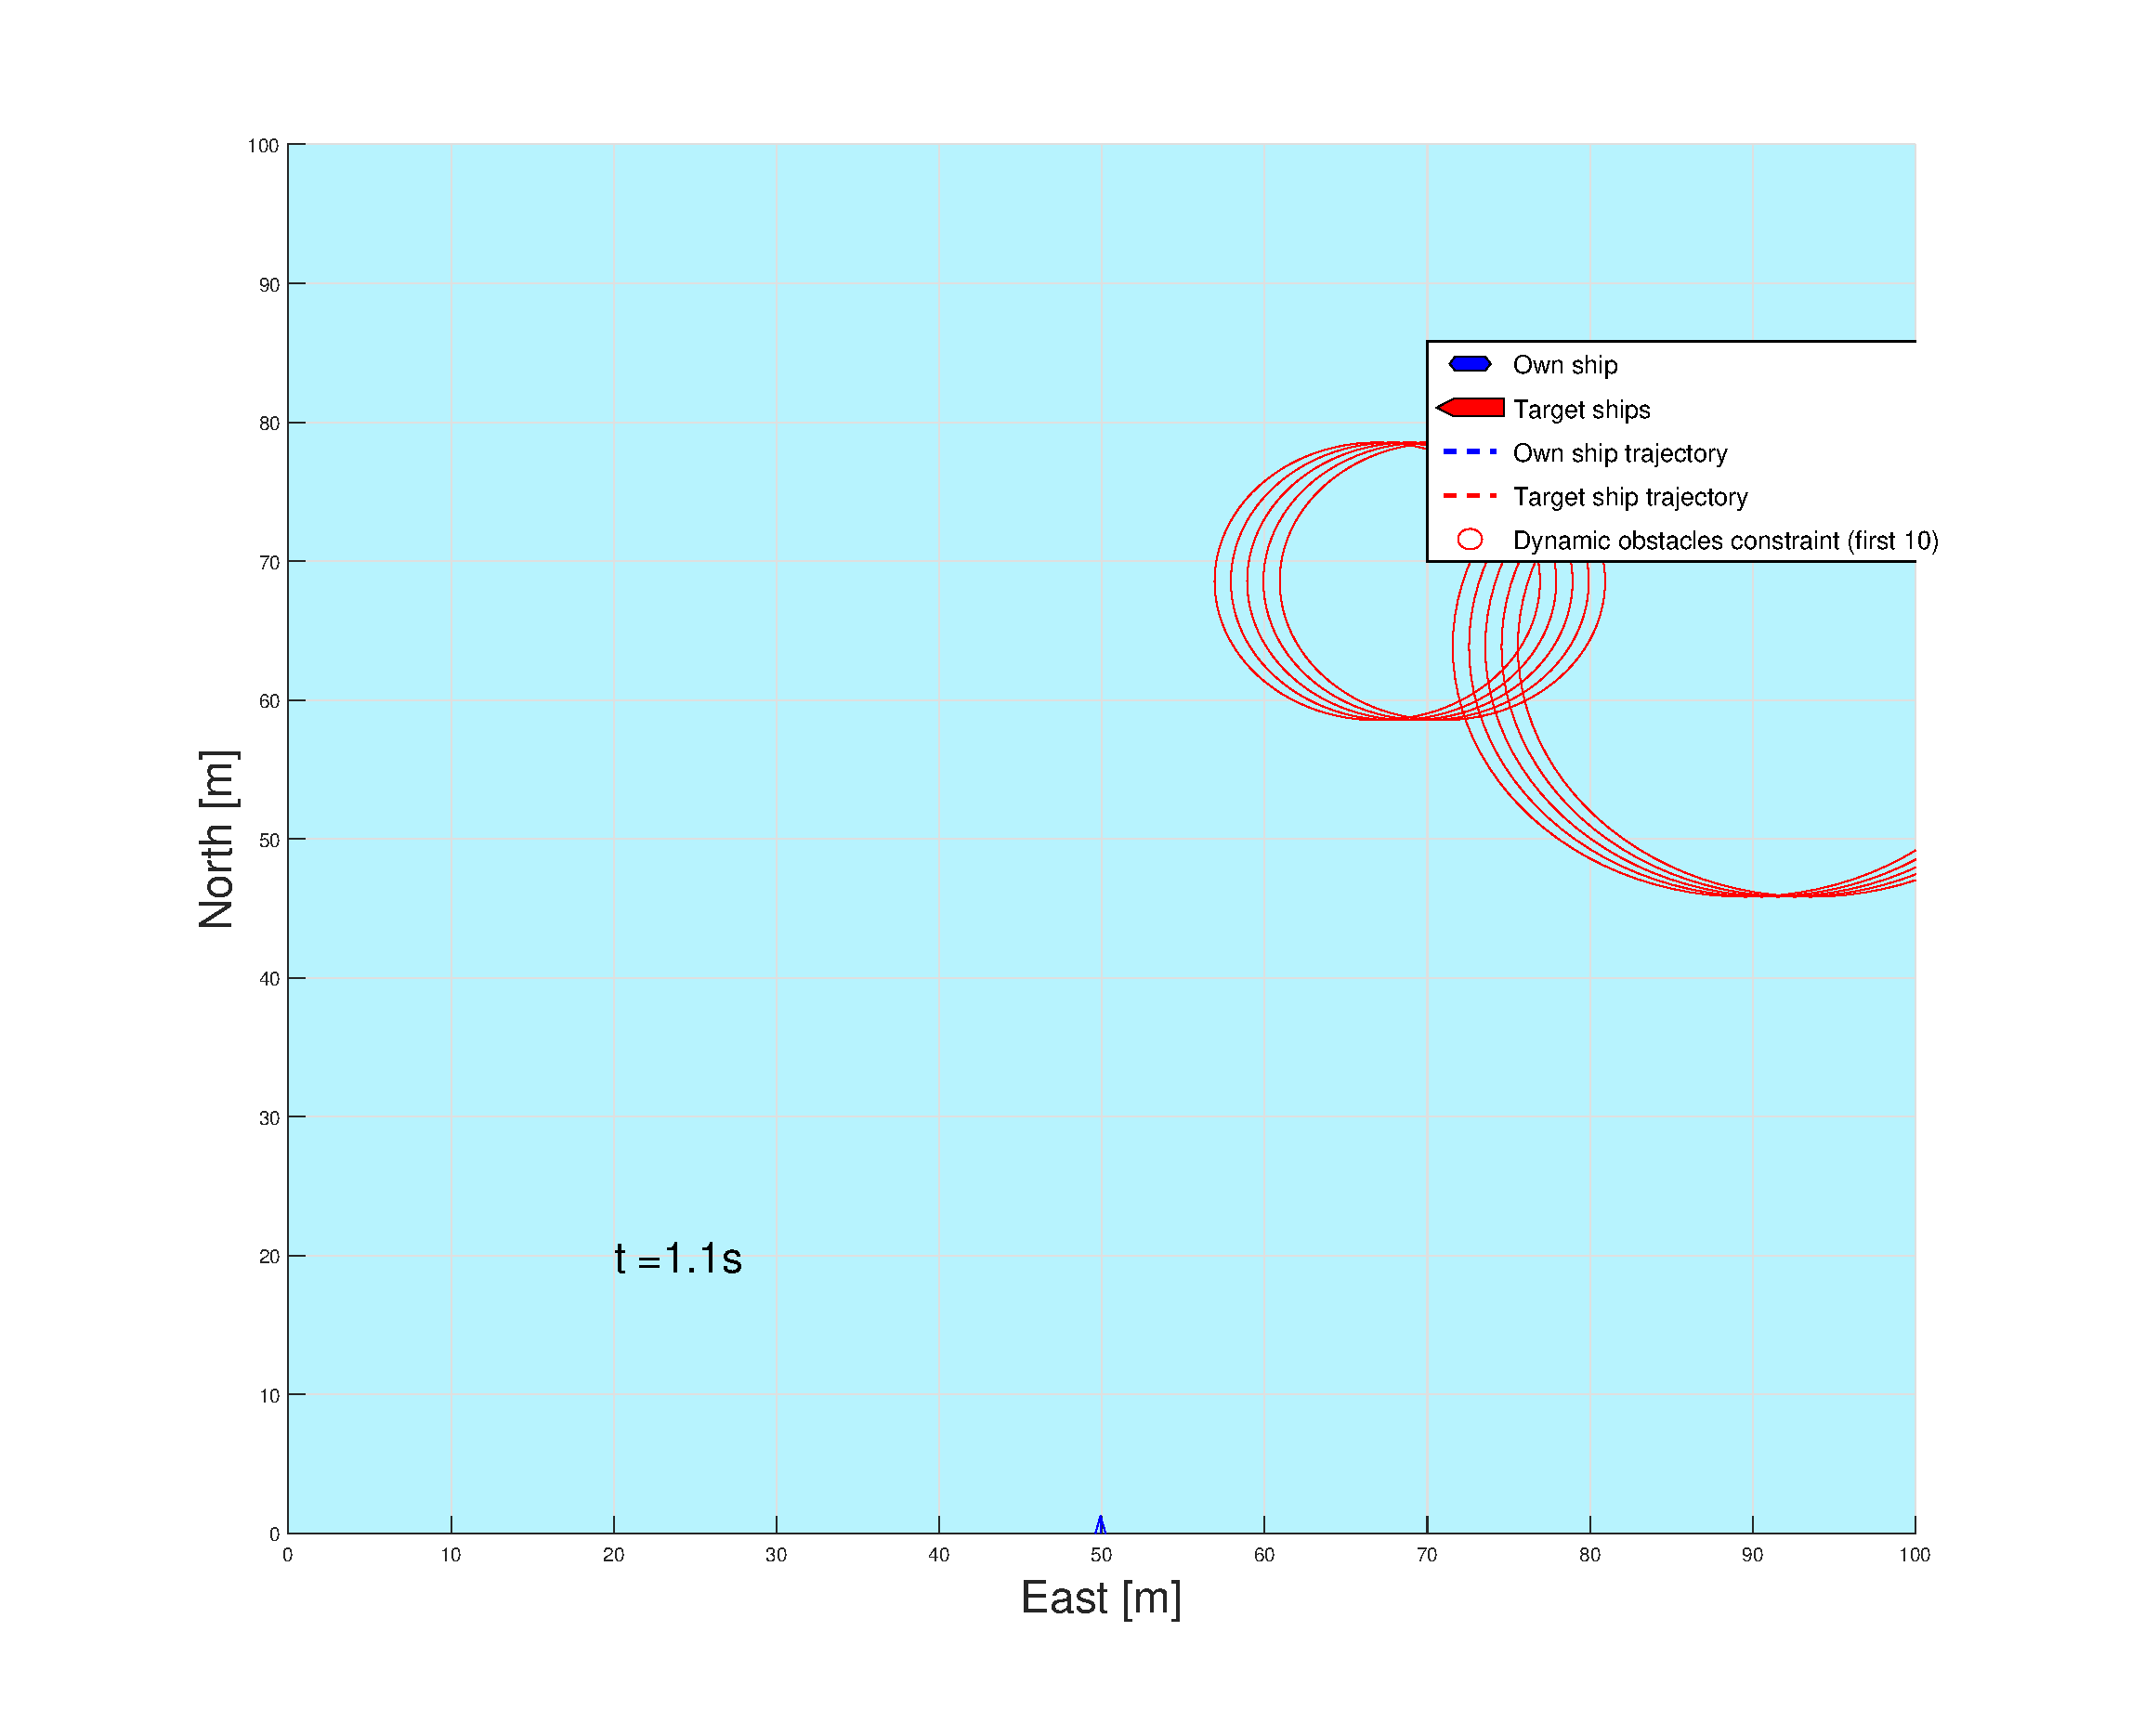
\includegraphics[width=\textwidth]{Images/Figures/enkel_GW/_Simple_1fig1_time=1}
%         \subcaption{}
%     \end{subfigure}
%     \hfill
%     \begin{subfigure}[b]{0.499\textwidth}
%         \centering
%         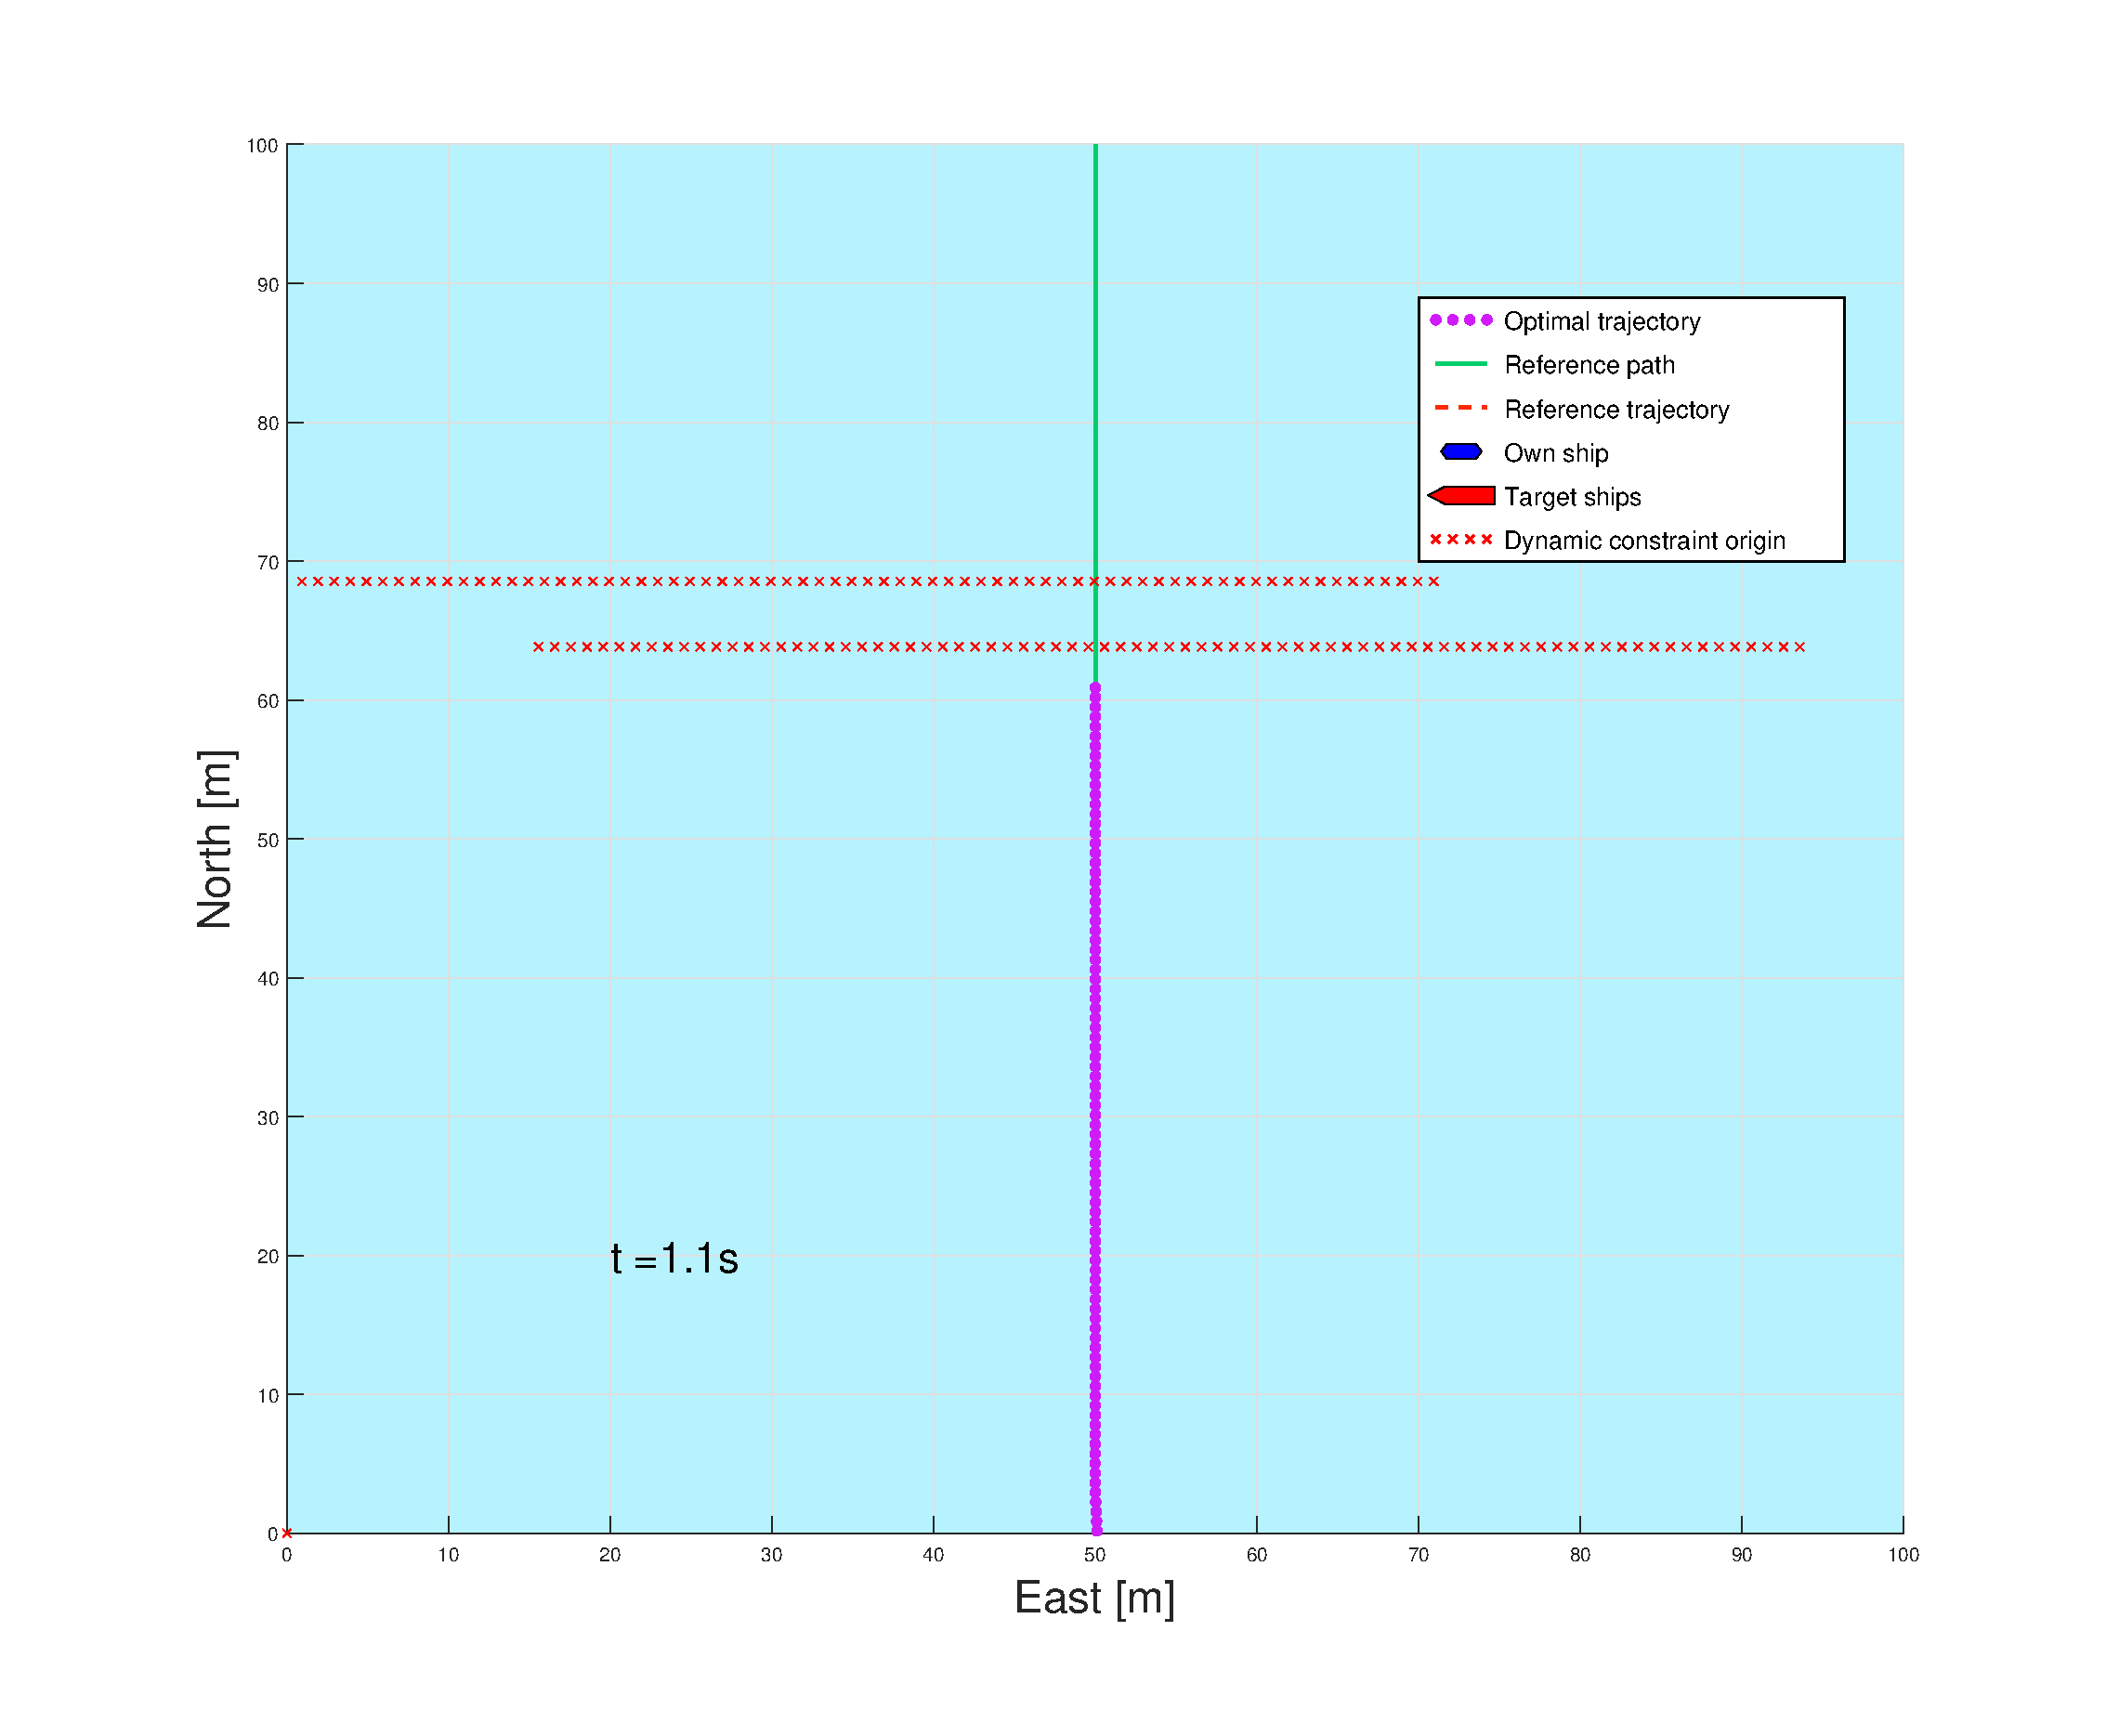
\includegraphics[width=\textwidth]{Images/Figures/enkel_GW/_Simple_1fig999_time=1}
%         \subcaption{}
%     \end{subfigure}
%     \hfill
%     \\
%     \begin{subfigure}[b]{0.49\textwidth}
%         \centering
%         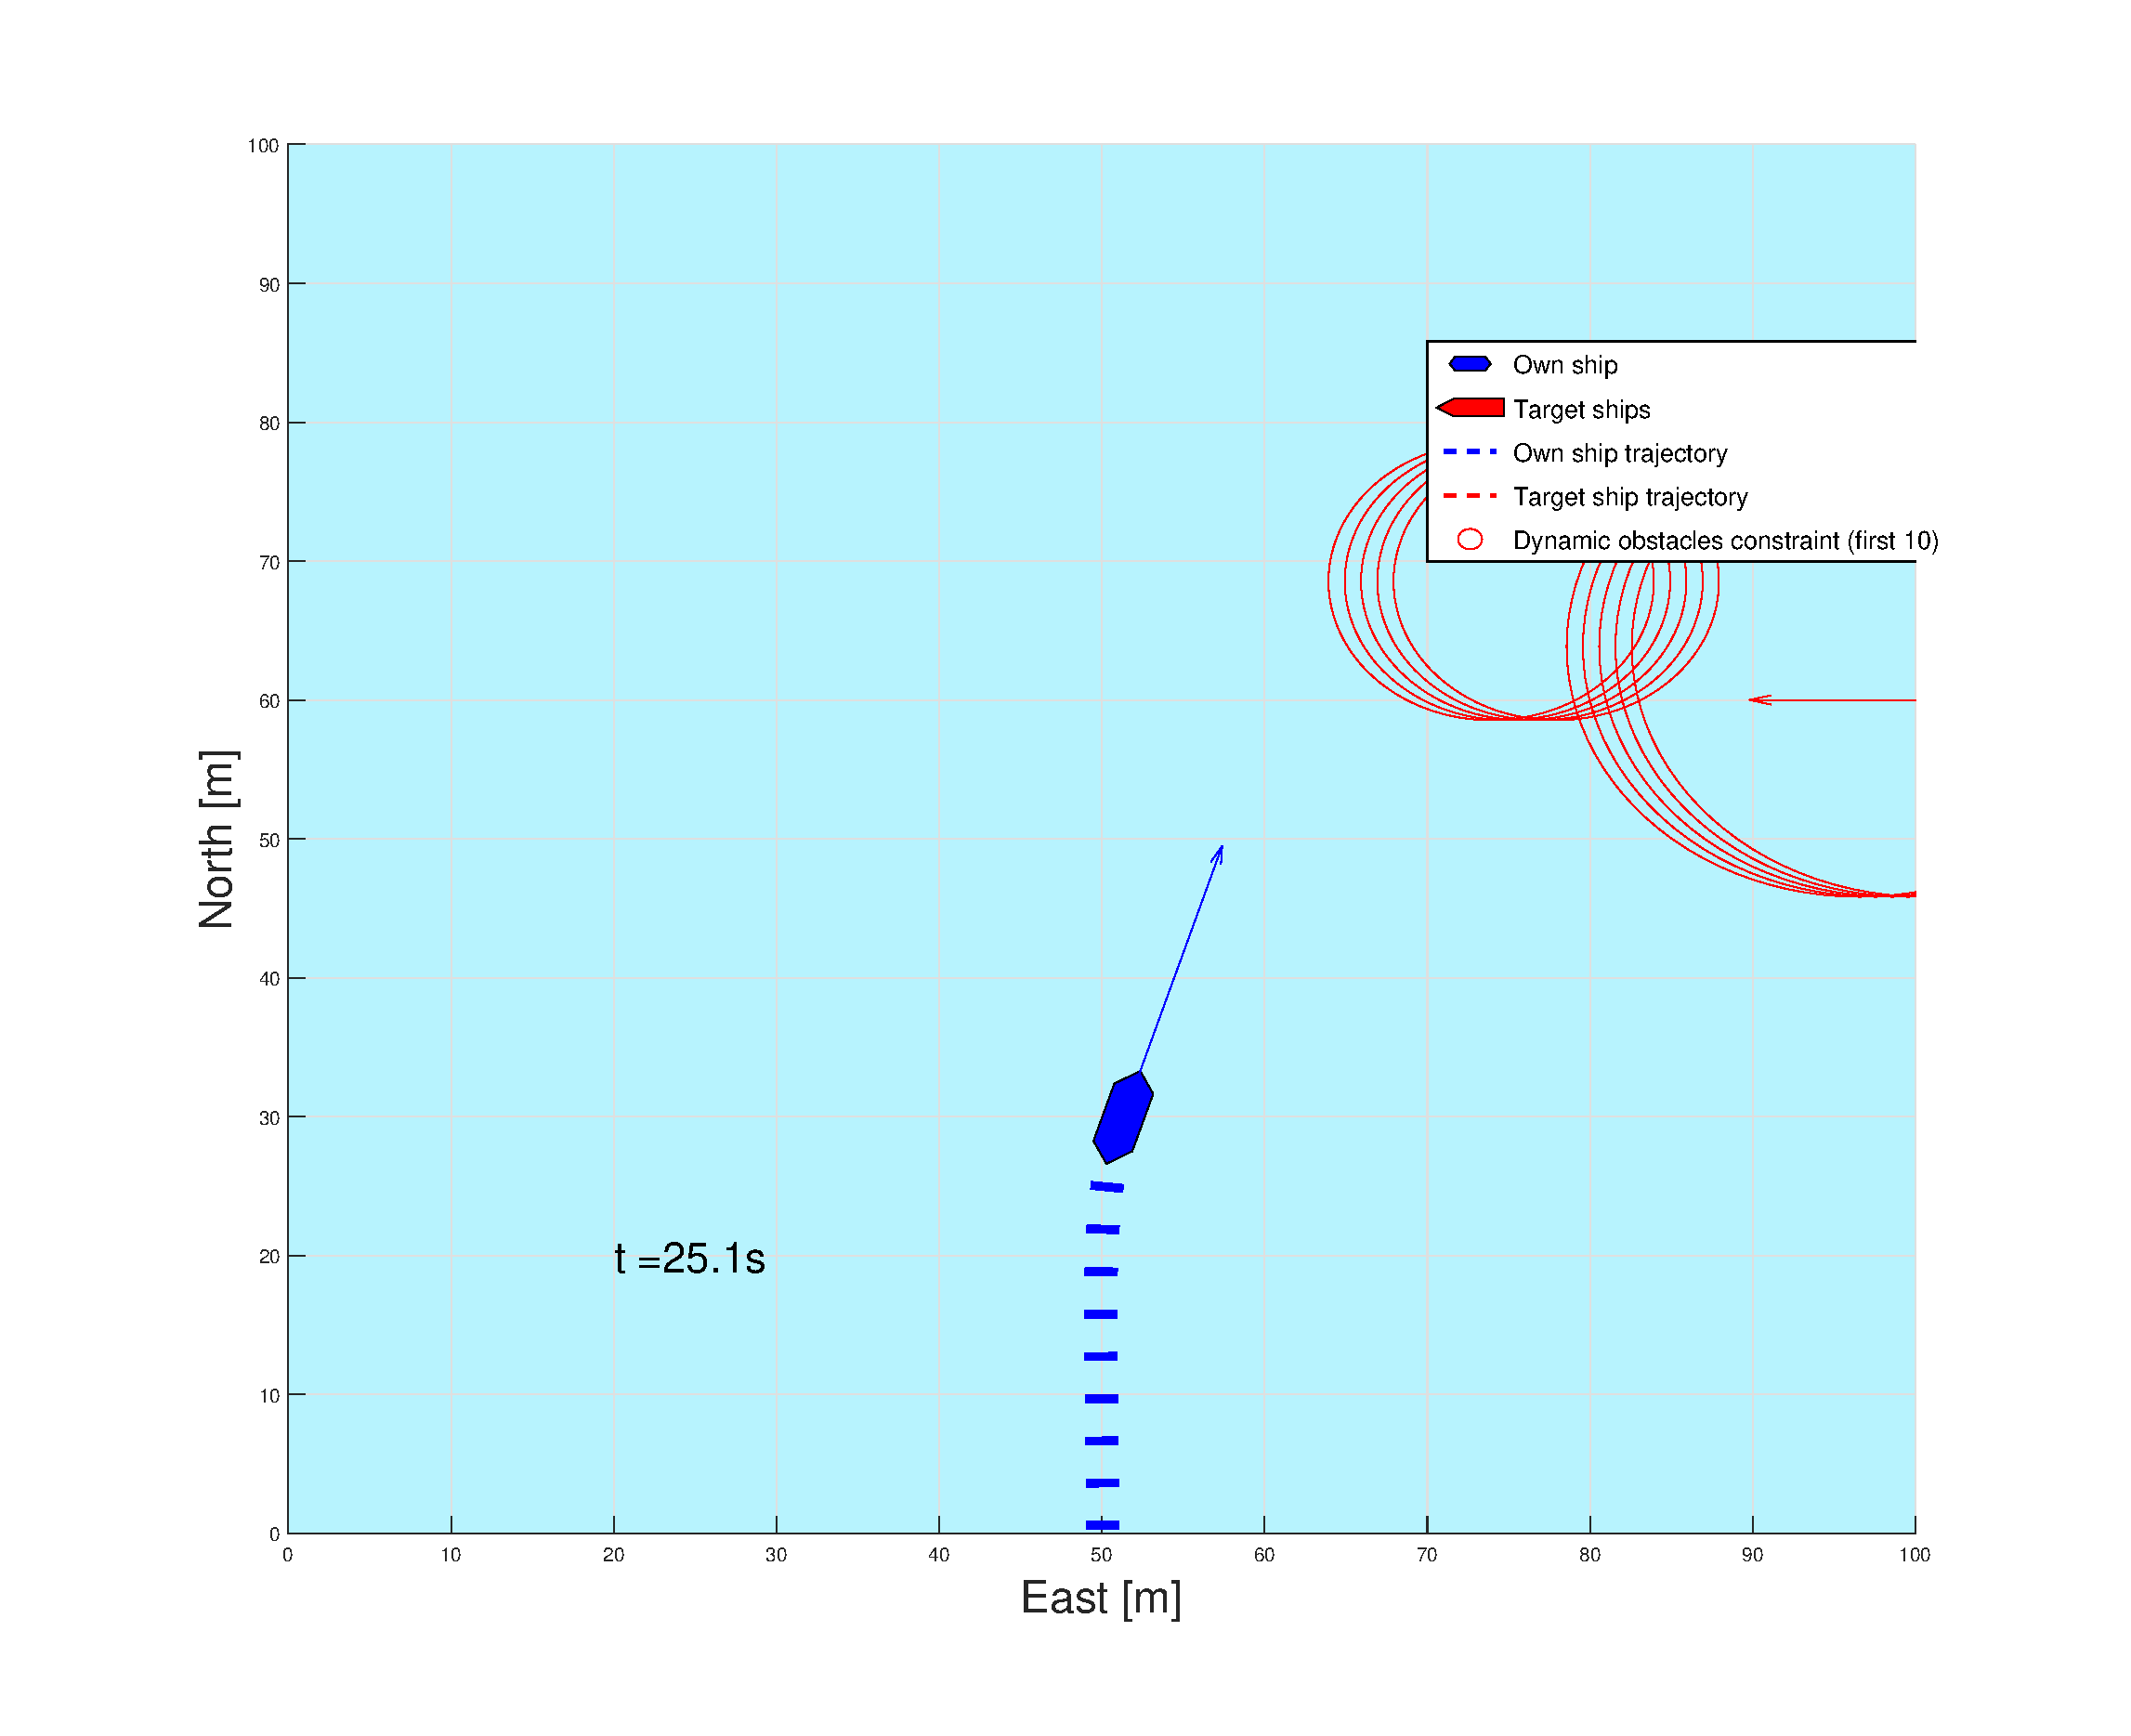
\includegraphics[width=\textwidth]{Images/Figures/enkel_GW/_Simple_1fig1_time=25}
%         \subcaption{}
%     \end{subfigure}
%     \hfill
%     \begin{subfigure}[b]{0.499\textwidth}
%         \centering
%         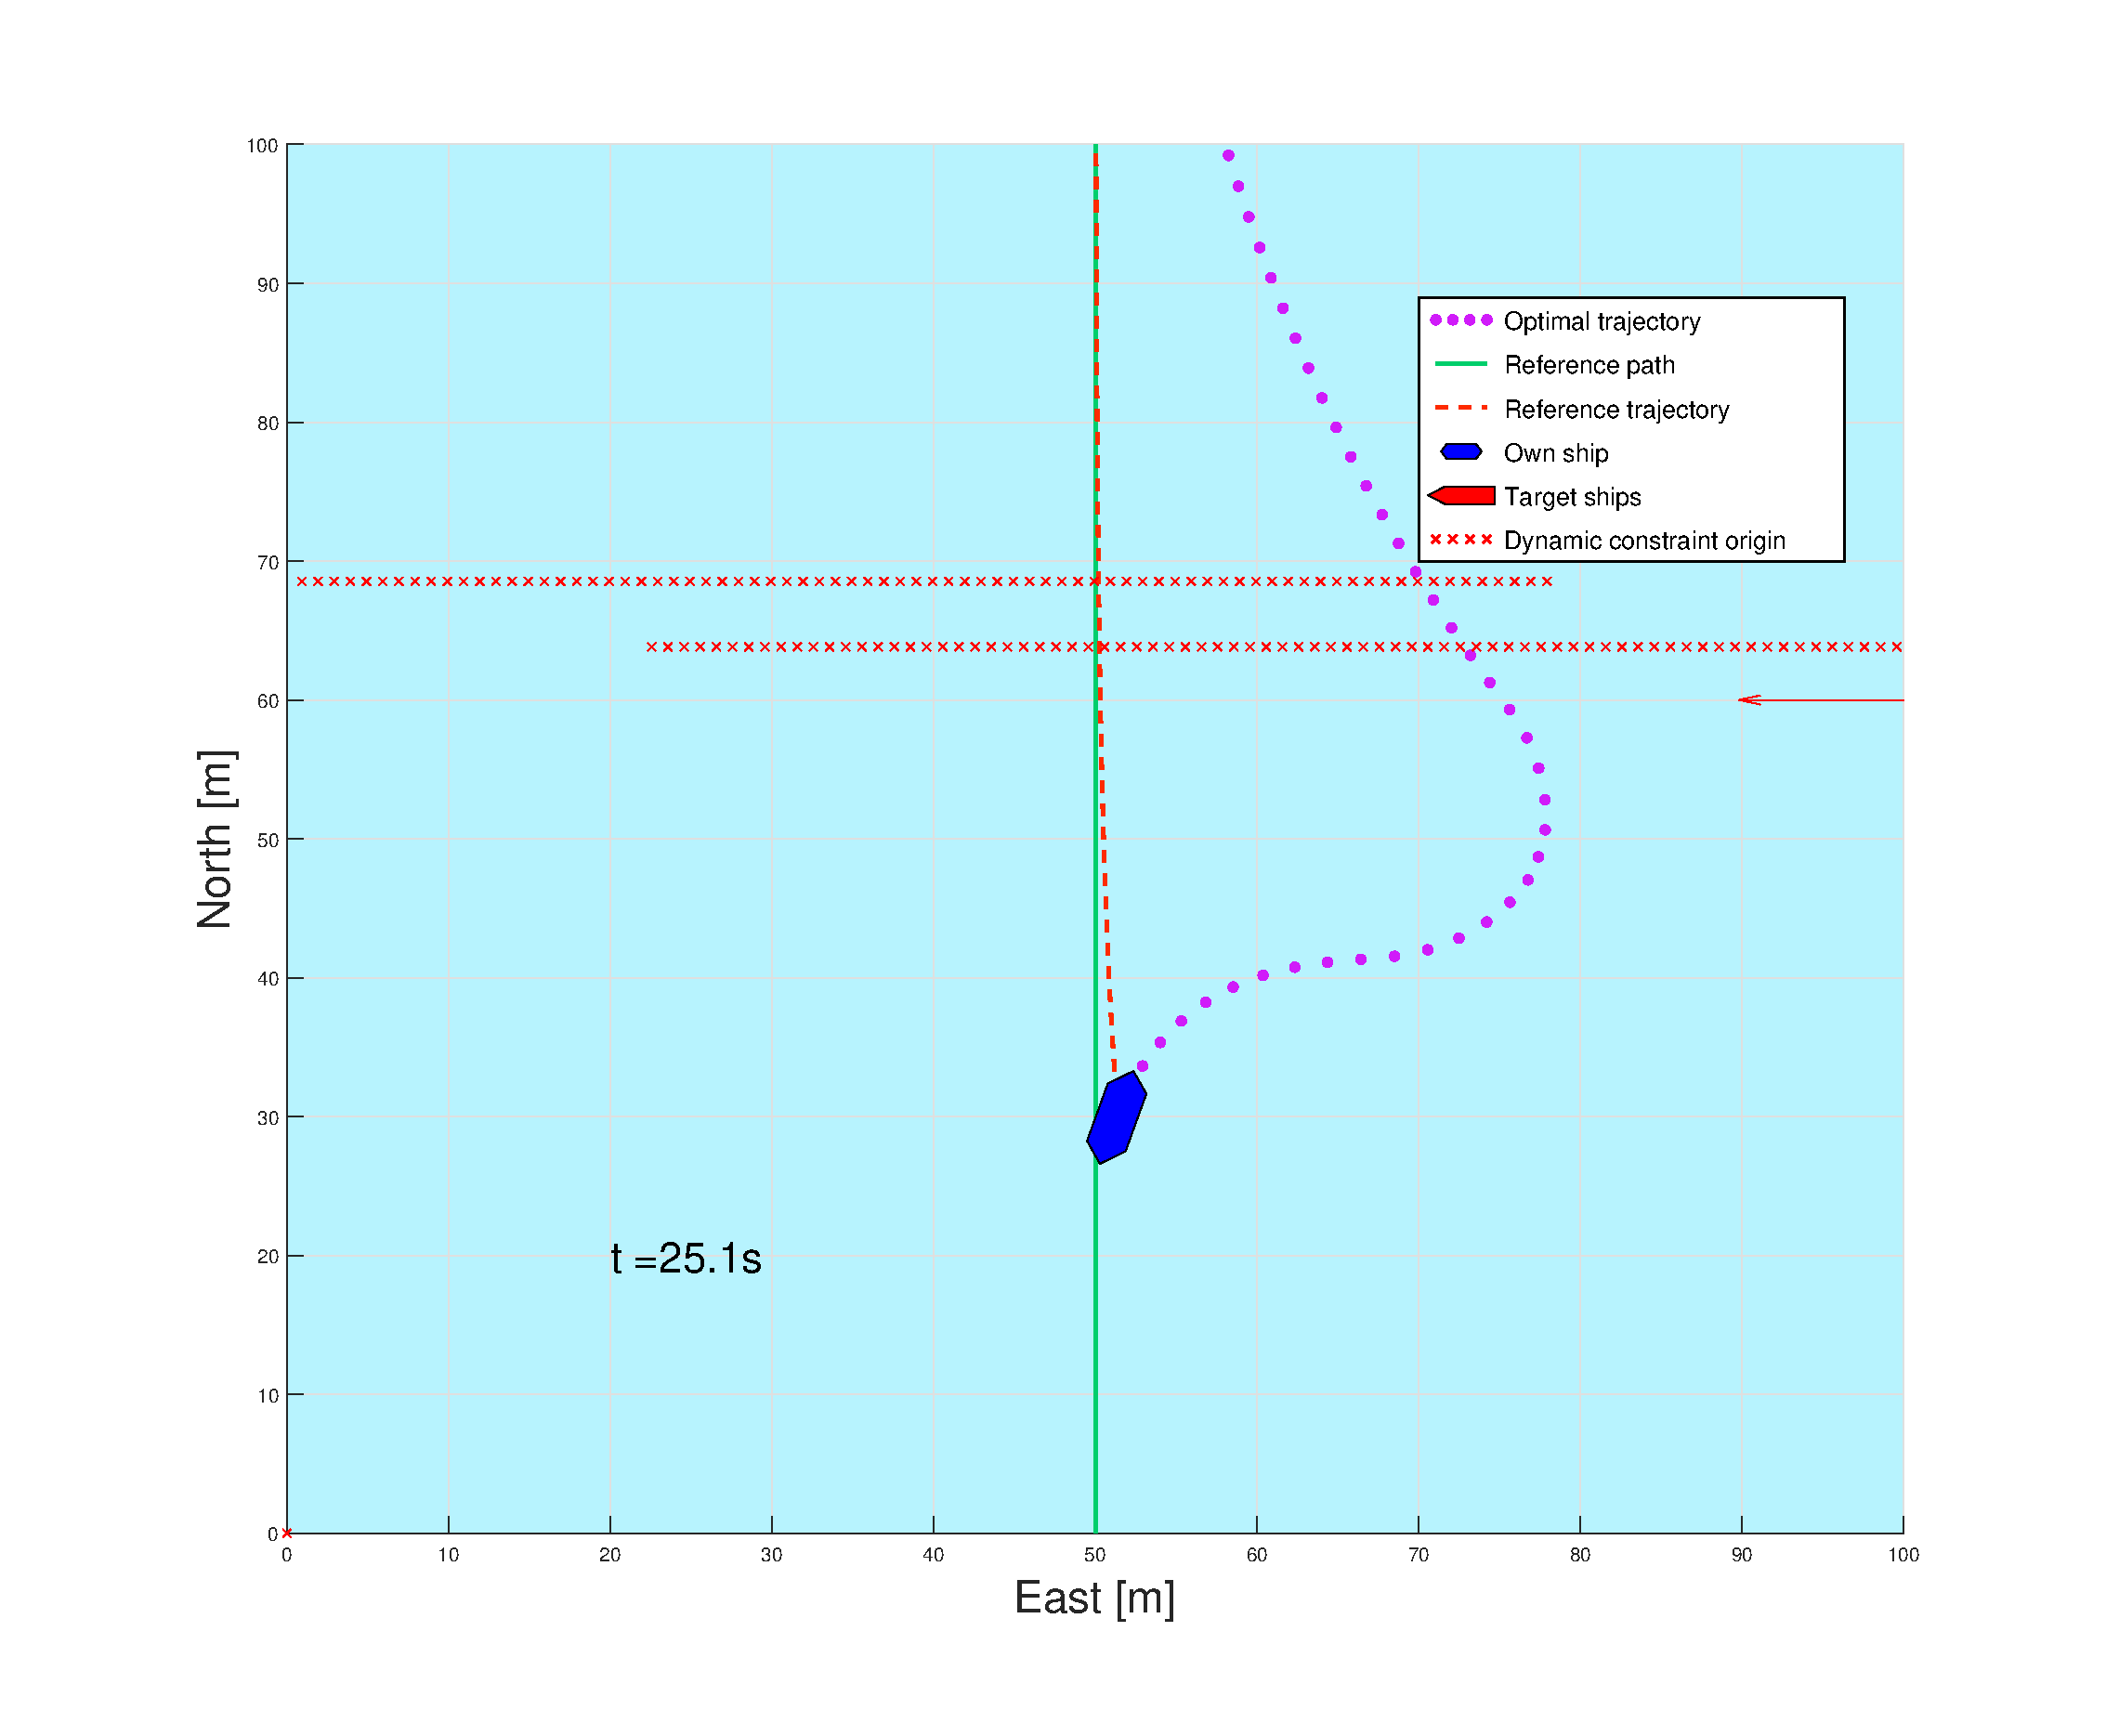
\includegraphics[width=\textwidth]{Images/Figures/enkel_GW/_Simple_1fig999_time=25}
%         \subcaption{}
%     \end{subfigure}
%     \hfill
% \end{figure}%
% \begin{figure}[ht]\ContinuedFloat
%     \begin{subfigure}[b]{0.49\textwidth}
%         \centering
%         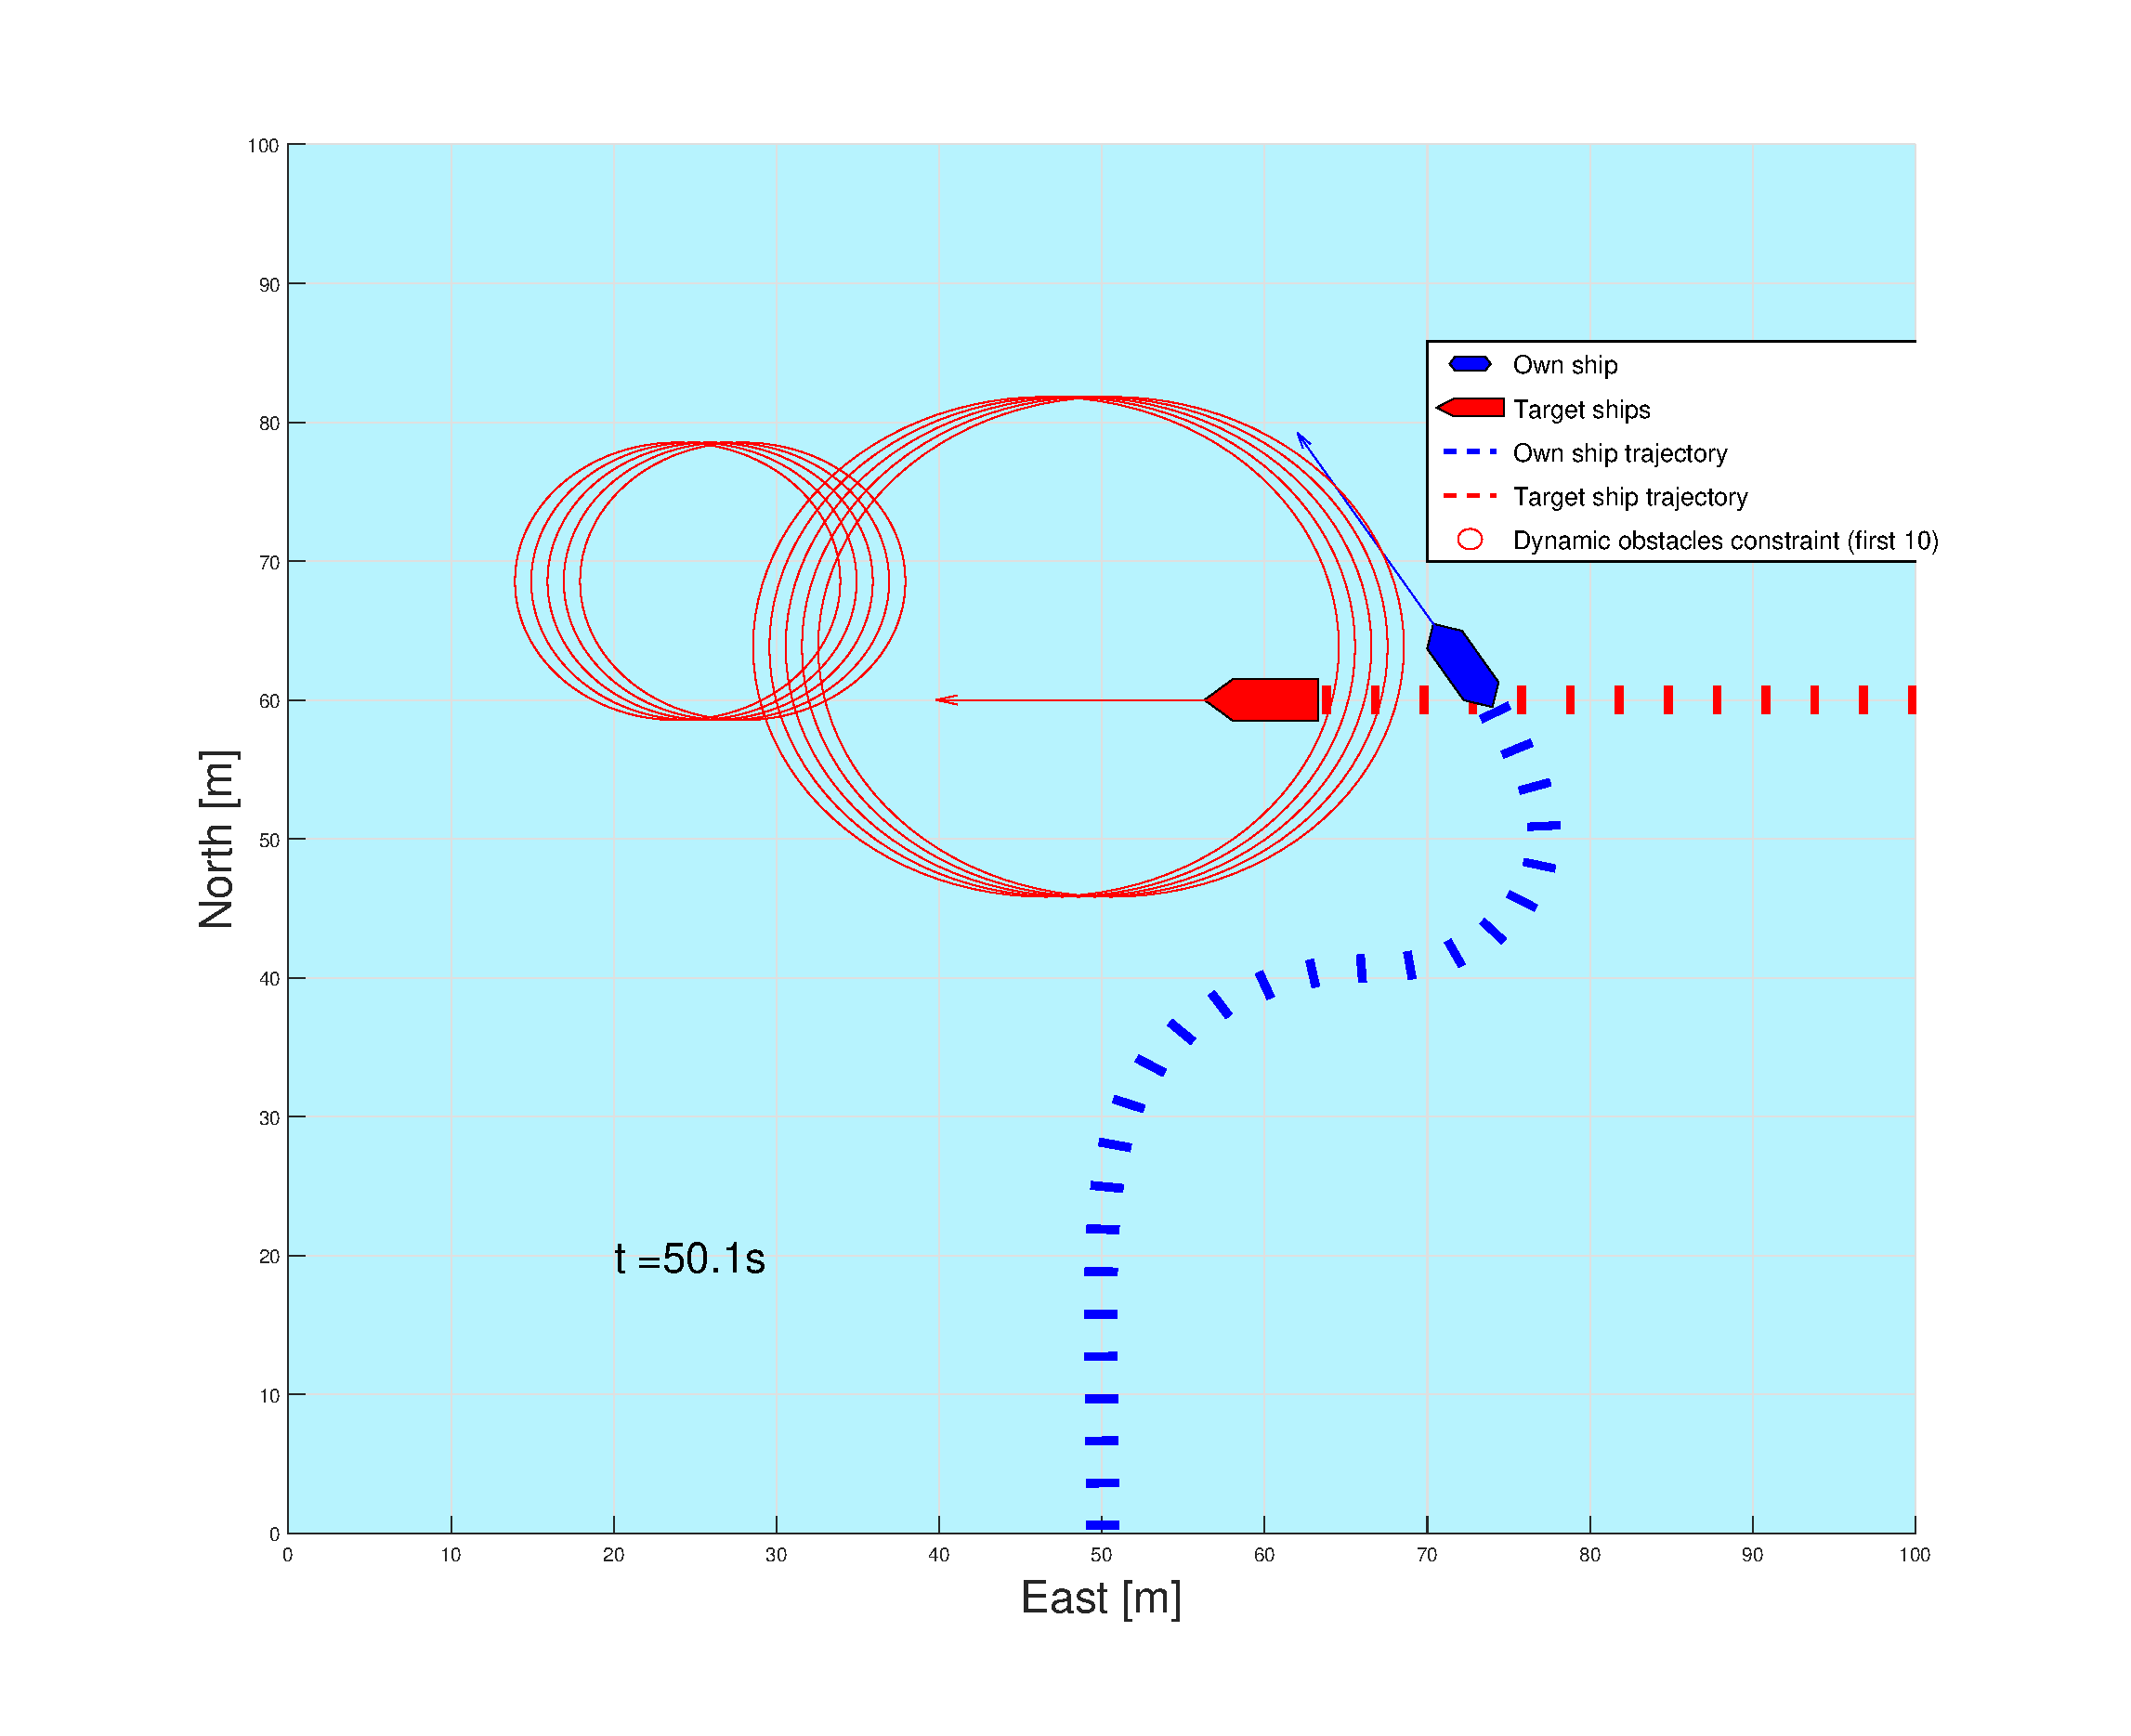
\includegraphics[width=\textwidth]{Images/Figures/enkel_GW/_Simple_1fig1_time=50}
%         \subcaption{}
%     \end{subfigure}
%     \hfill
%     \begin{subfigure}[b]{0.499\textwidth}
%         \centering
%         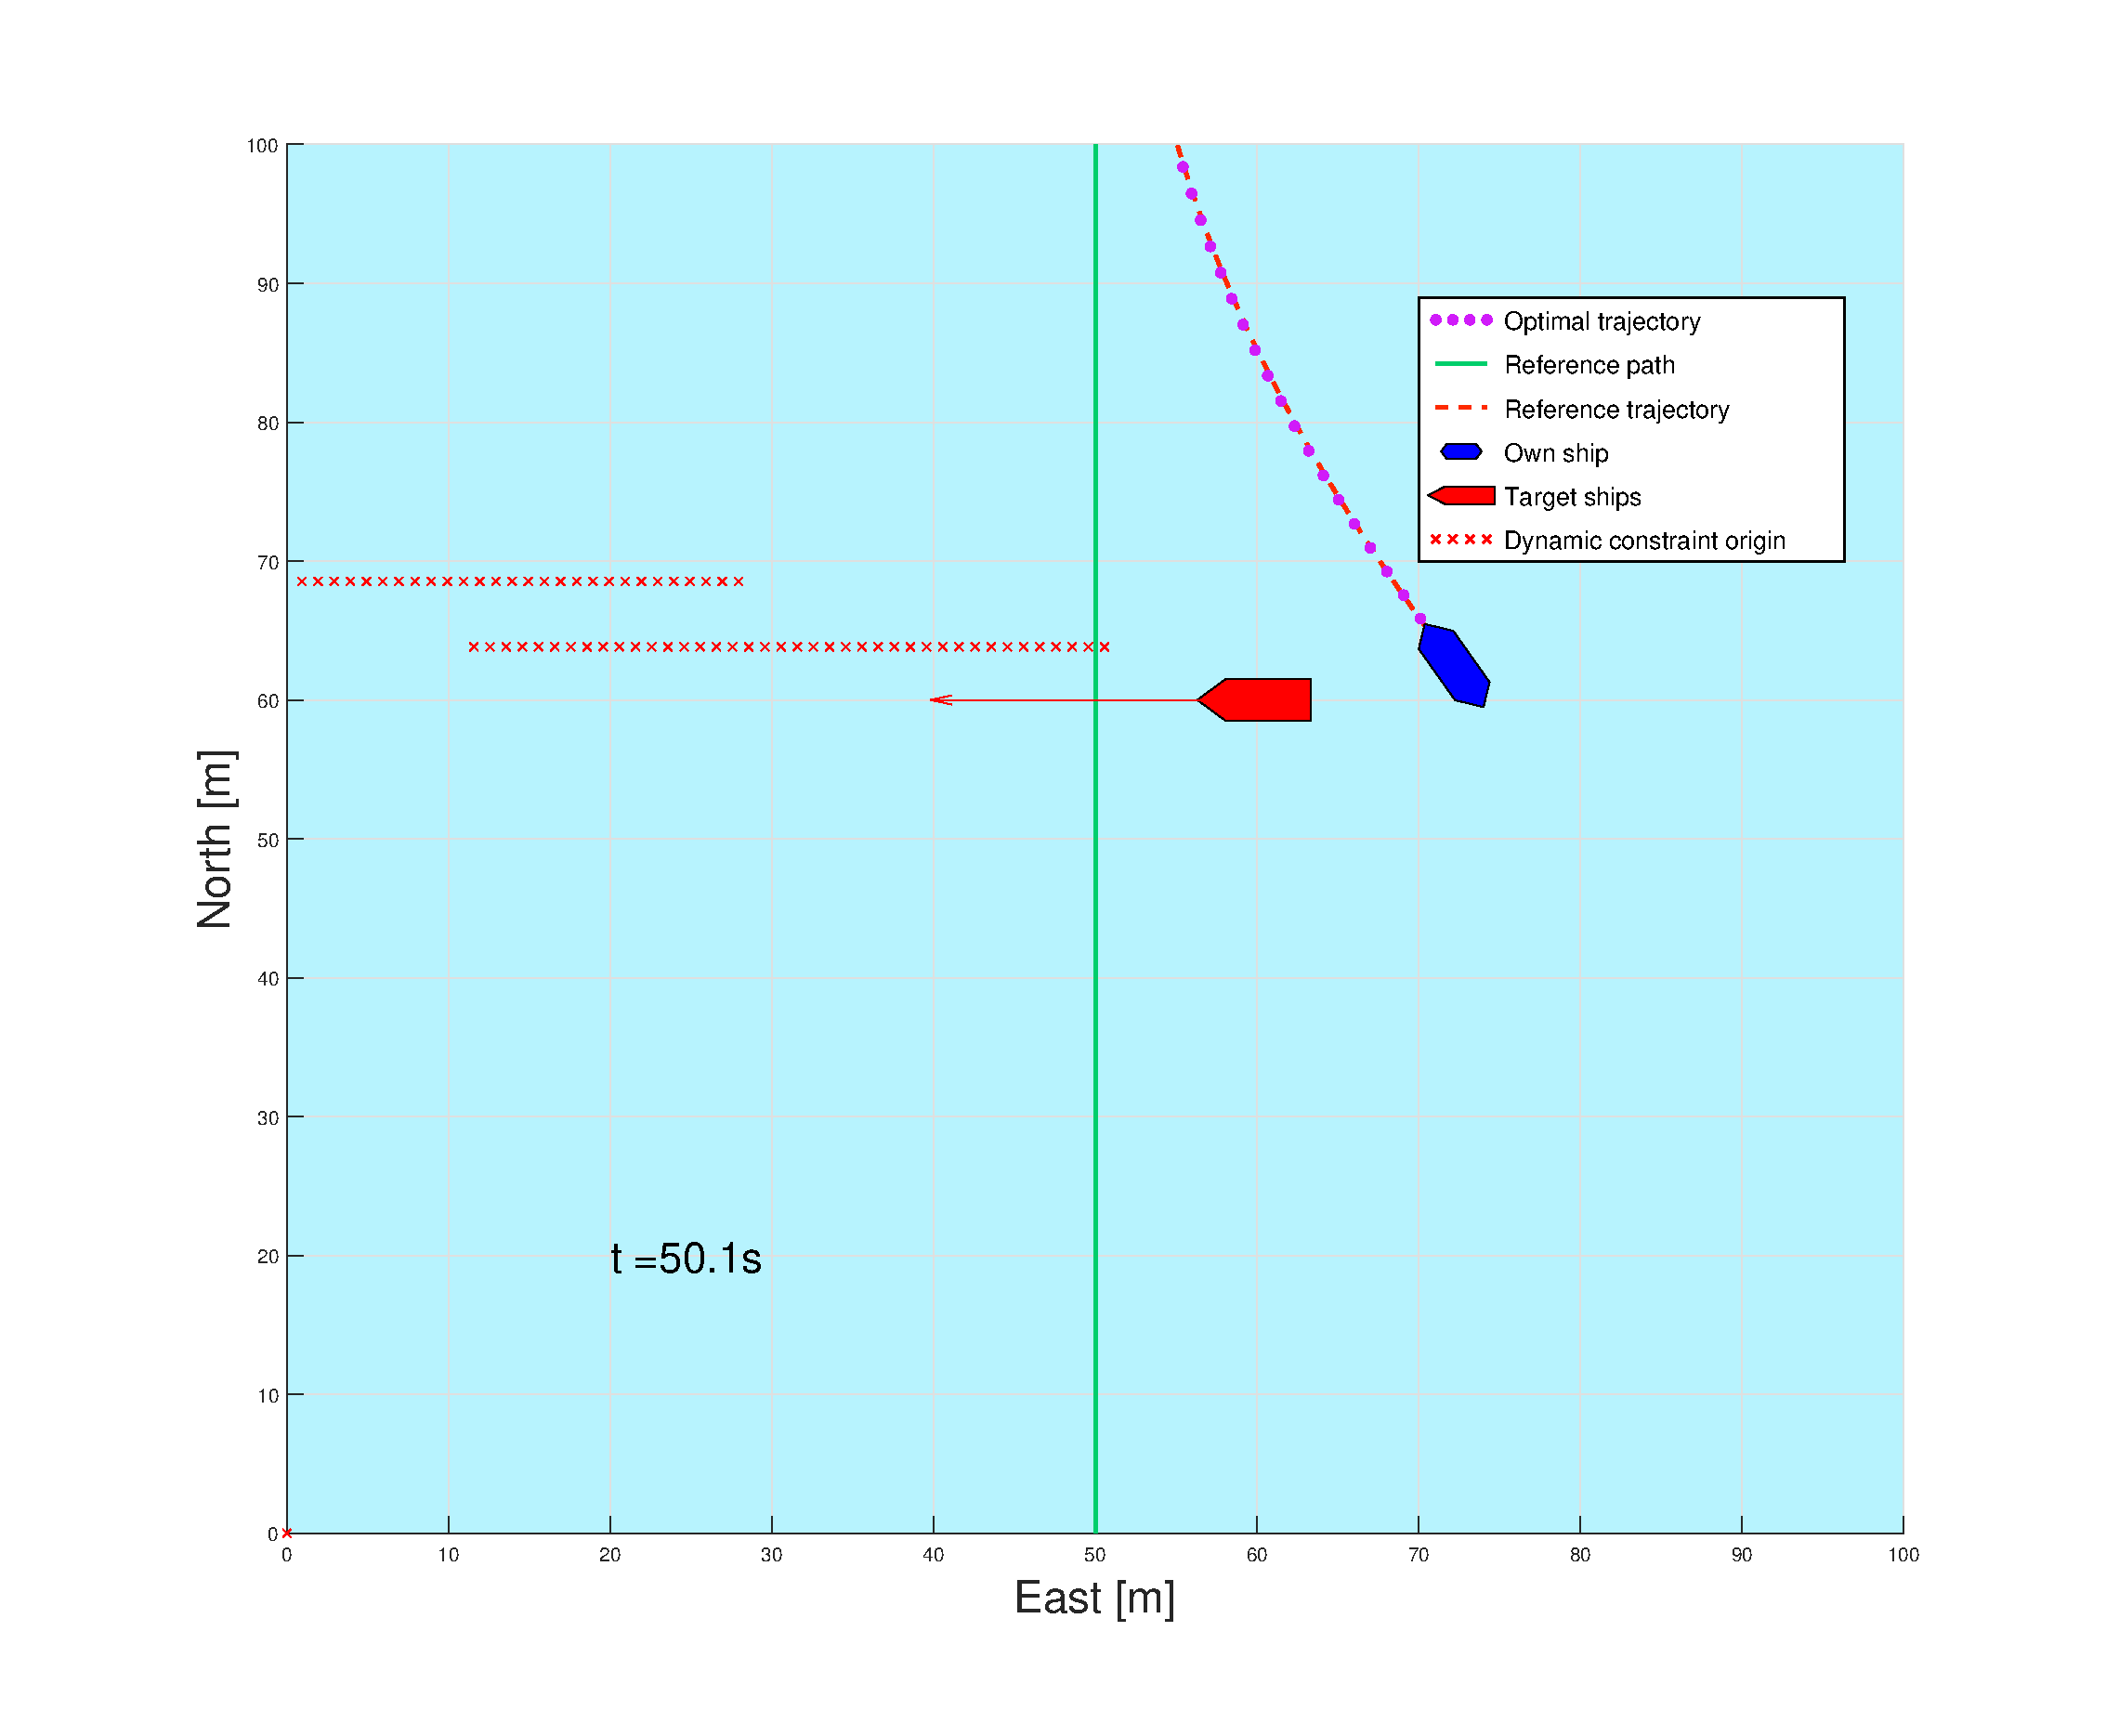
\includegraphics[width=\textwidth]{Images/Figures/enkel_GW/_Simple_1fig999_time=50}
%         \subcaption{}
%     \end{subfigure}
%     \hfill
%     \\
%     \begin{subfigure}[b]{0.49\textwidth}
%         \centering
%         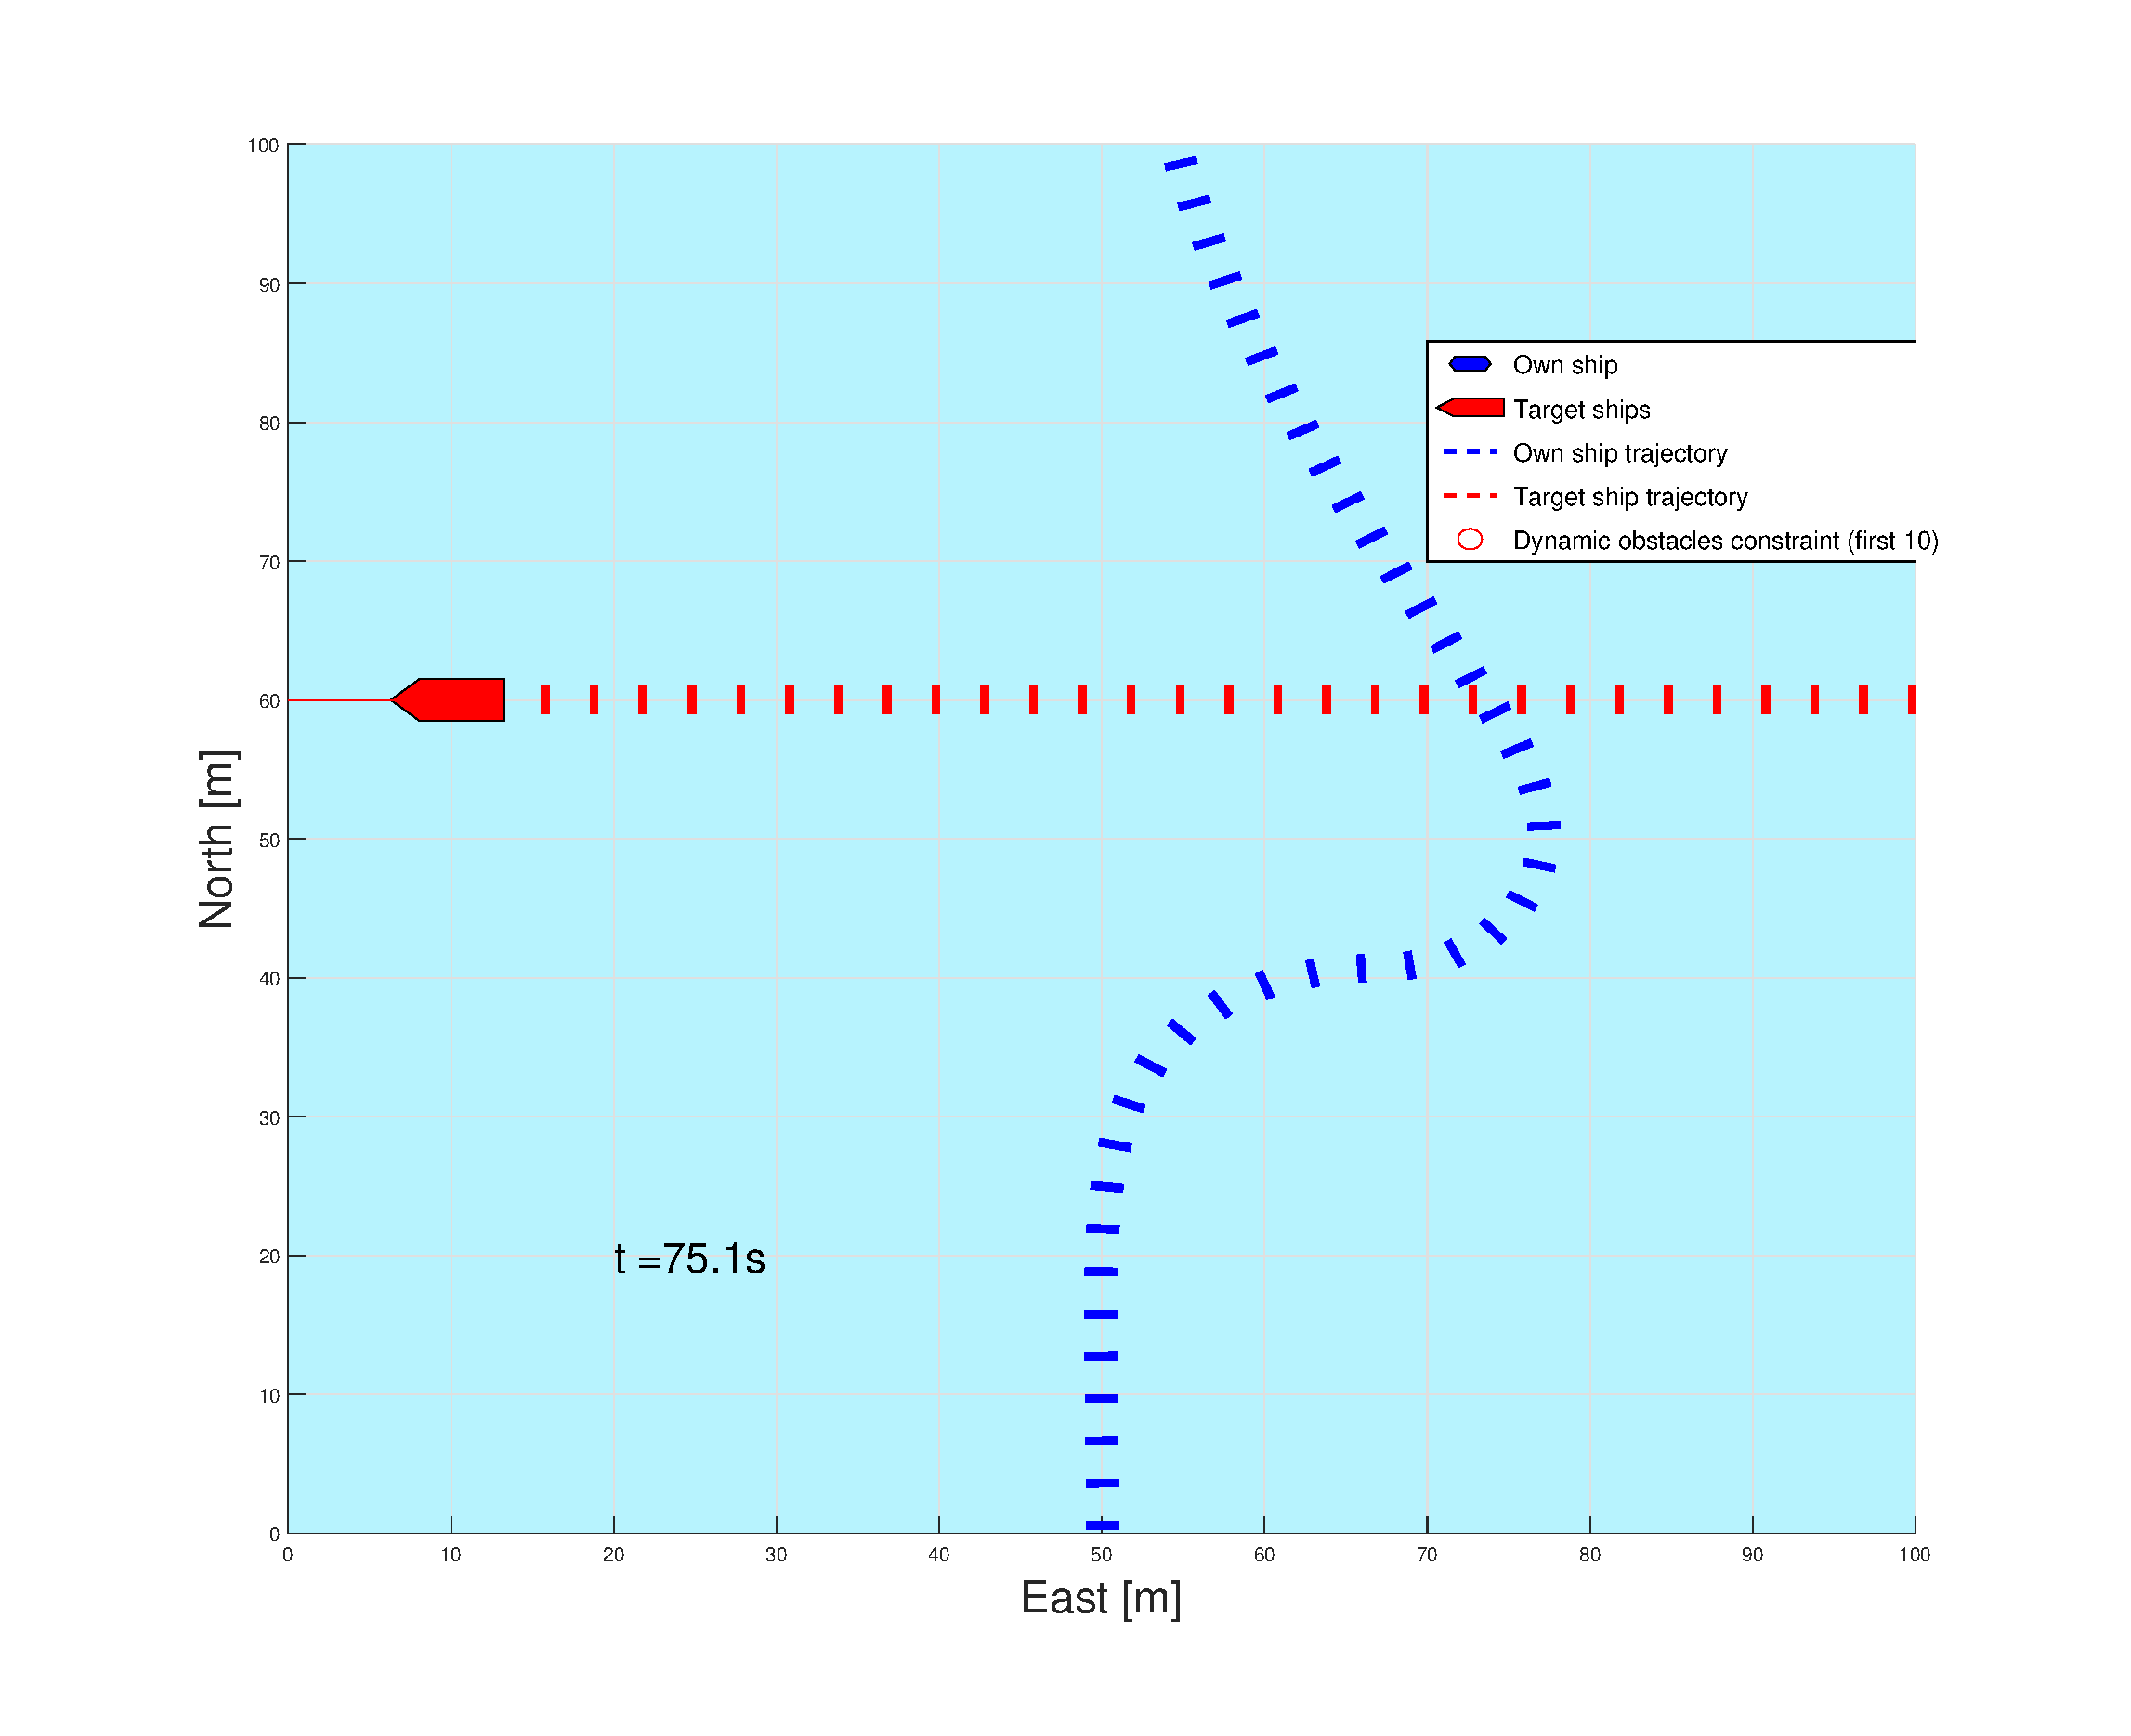
\includegraphics[width=\textwidth]{Images/Figures/enkel_GW/_Simple_1fig1_time=75}
%         \subcaption{}
%     \end{subfigure}
%     \hfill
%     \begin{subfigure}[b]{0.499\textwidth}
%         \centering
%         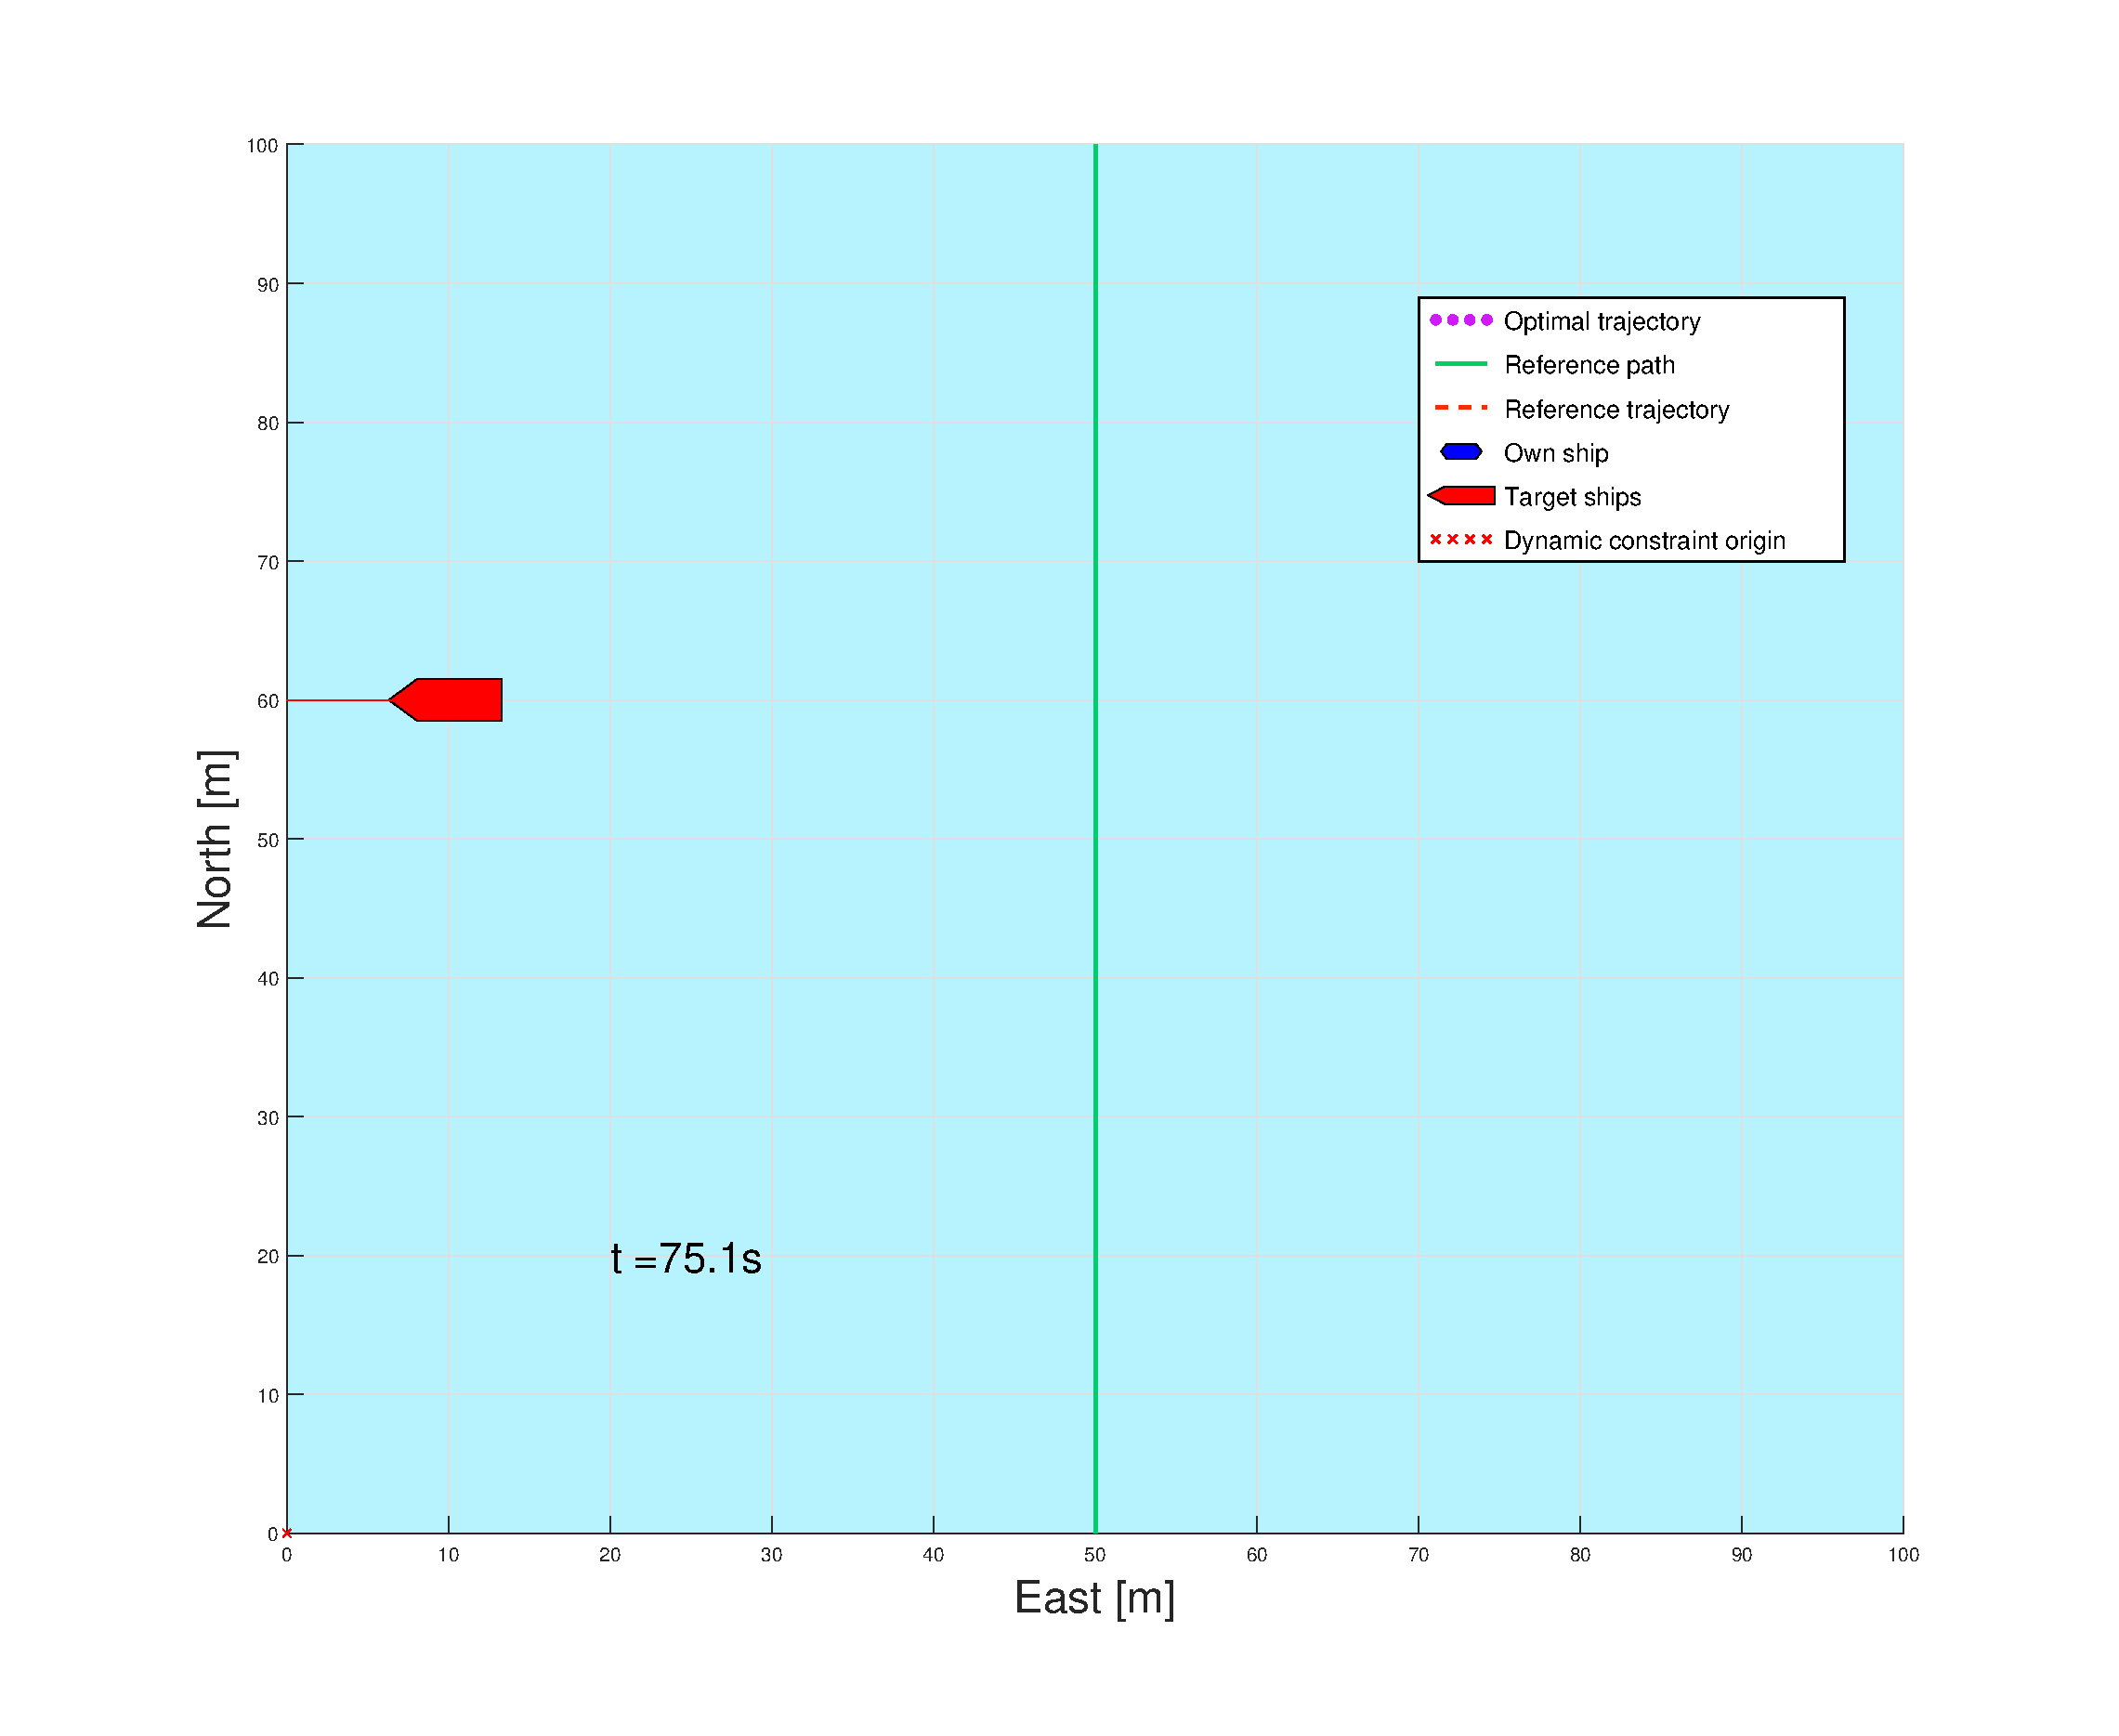
\includegraphics[width=\textwidth]{Images/Figures/enkel_GW/_Simple_1fig999_time=75}
%         \subcaption{}
%     \end{subfigure}
%     \hfill
%     \caption{Simple Give Way Without Prediction}
% \end{figure}

\begin{figure}[ht!] % Simple Stand On, with prediction
    % \begin{subfigure}[b]{0.49\textwidth}
    %     \centering
    %     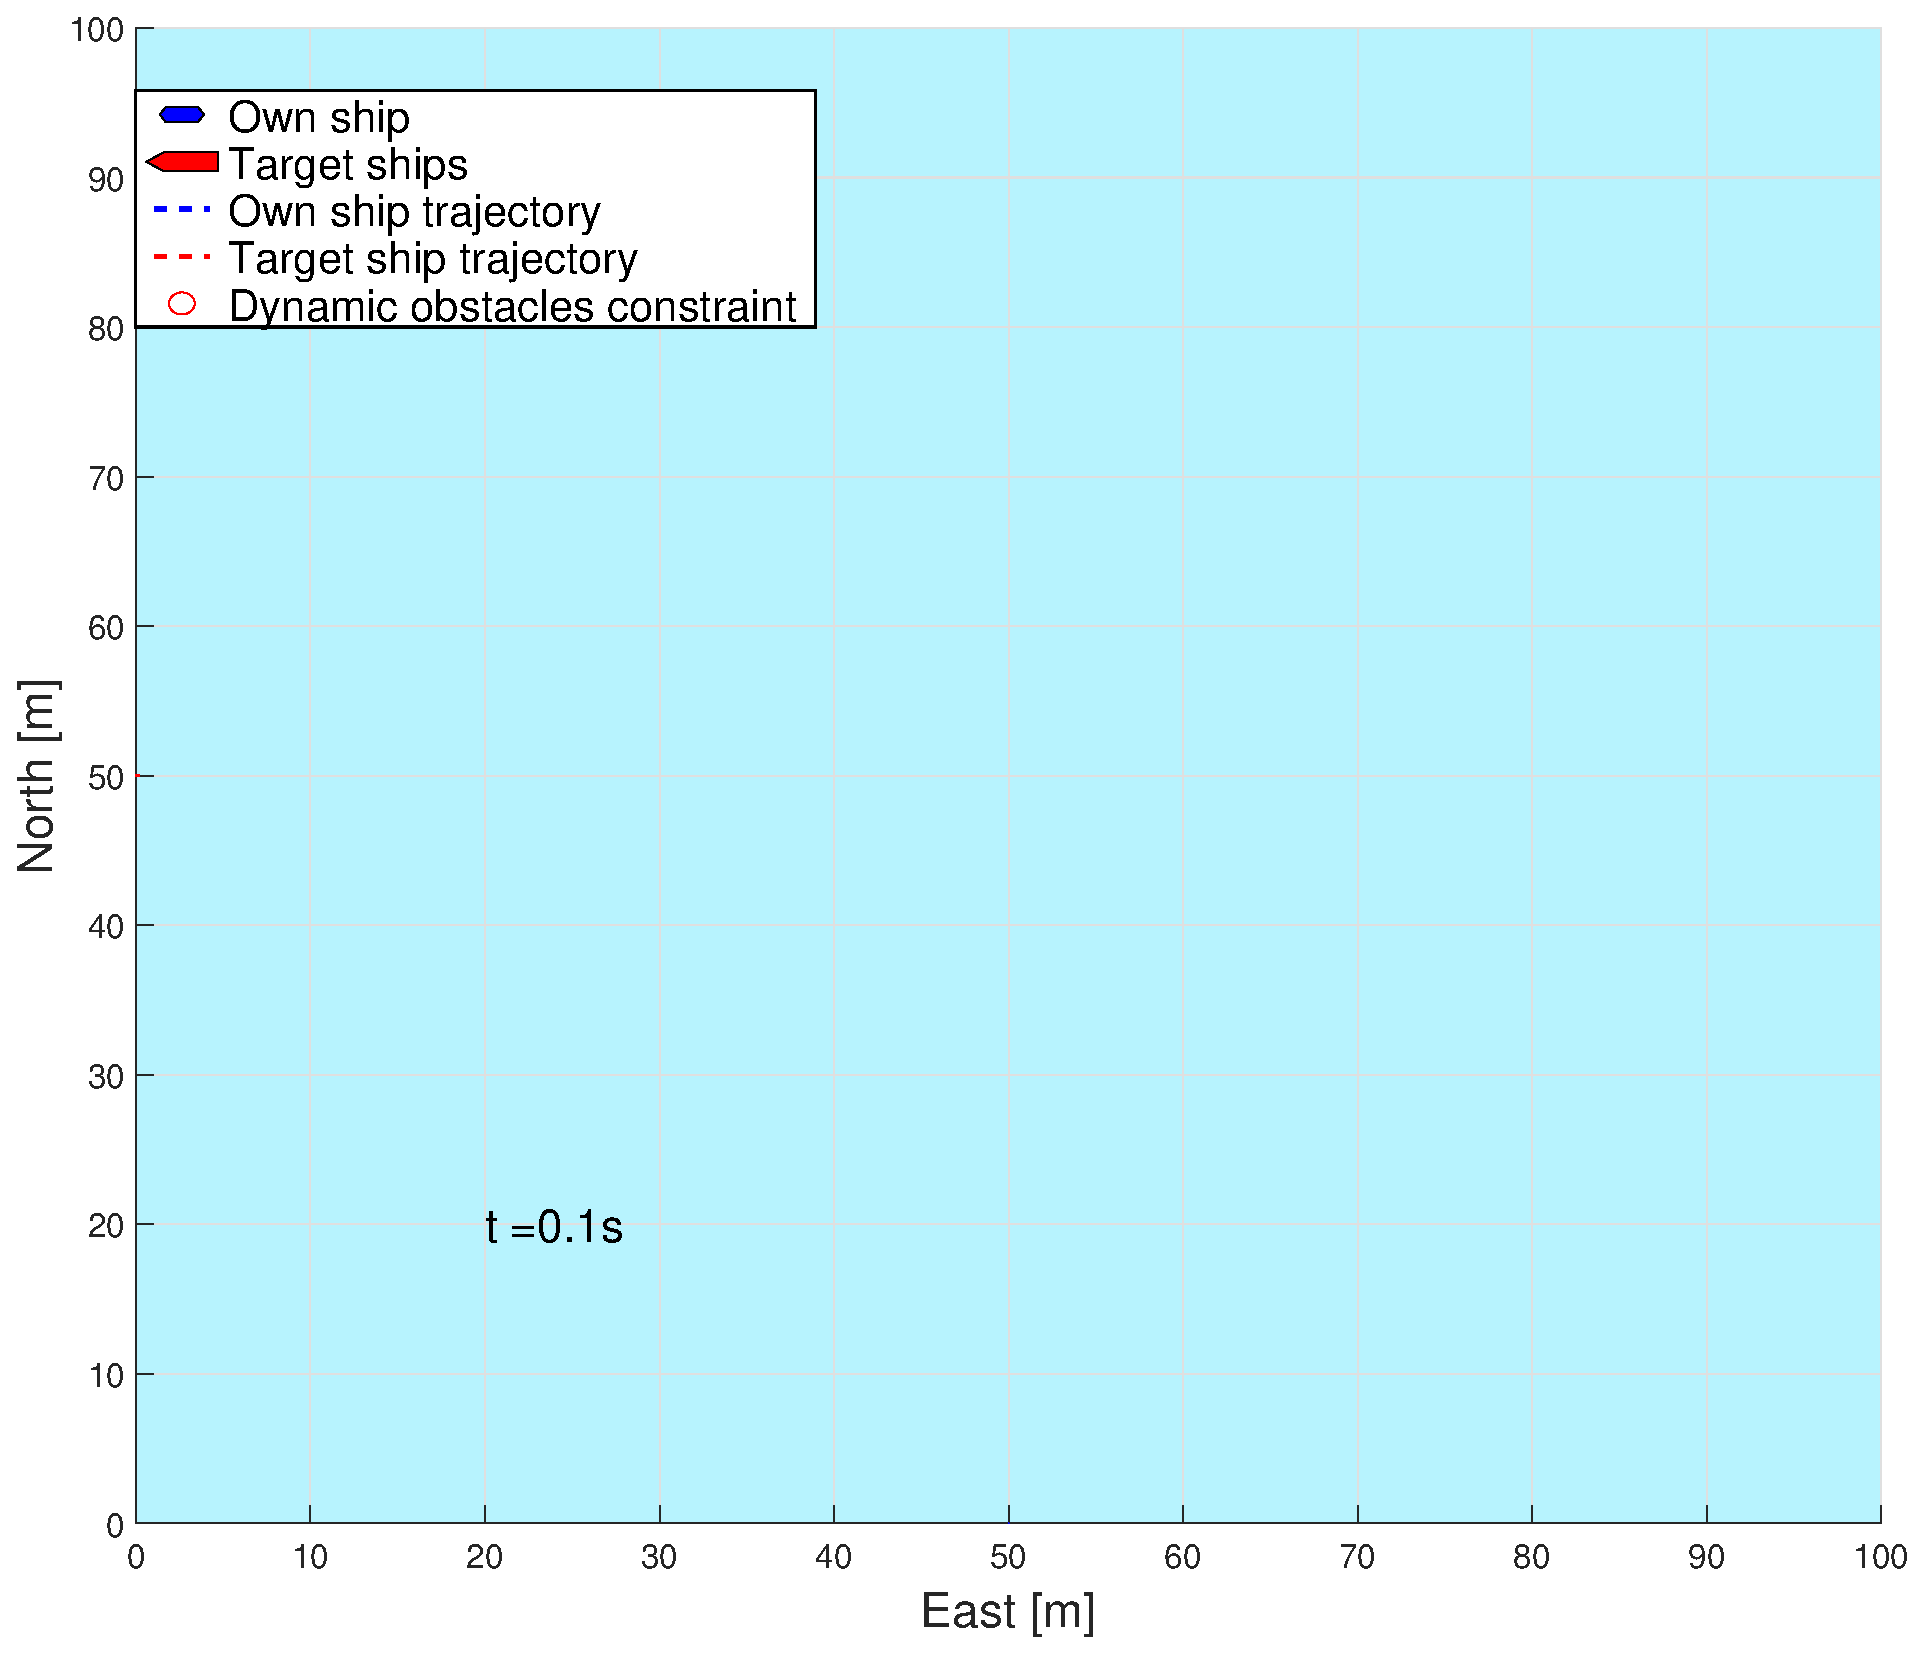
\includegraphics[width=\textwidth]{Images/Figures/enkel_SO/_Simple_0fig1_time=0}
    %     \subcaption{}
    % \end{subfigure}
    % \hfill
    % \begin{subfigure}[b]{0.499\textwidth}
    %     \centering
    %     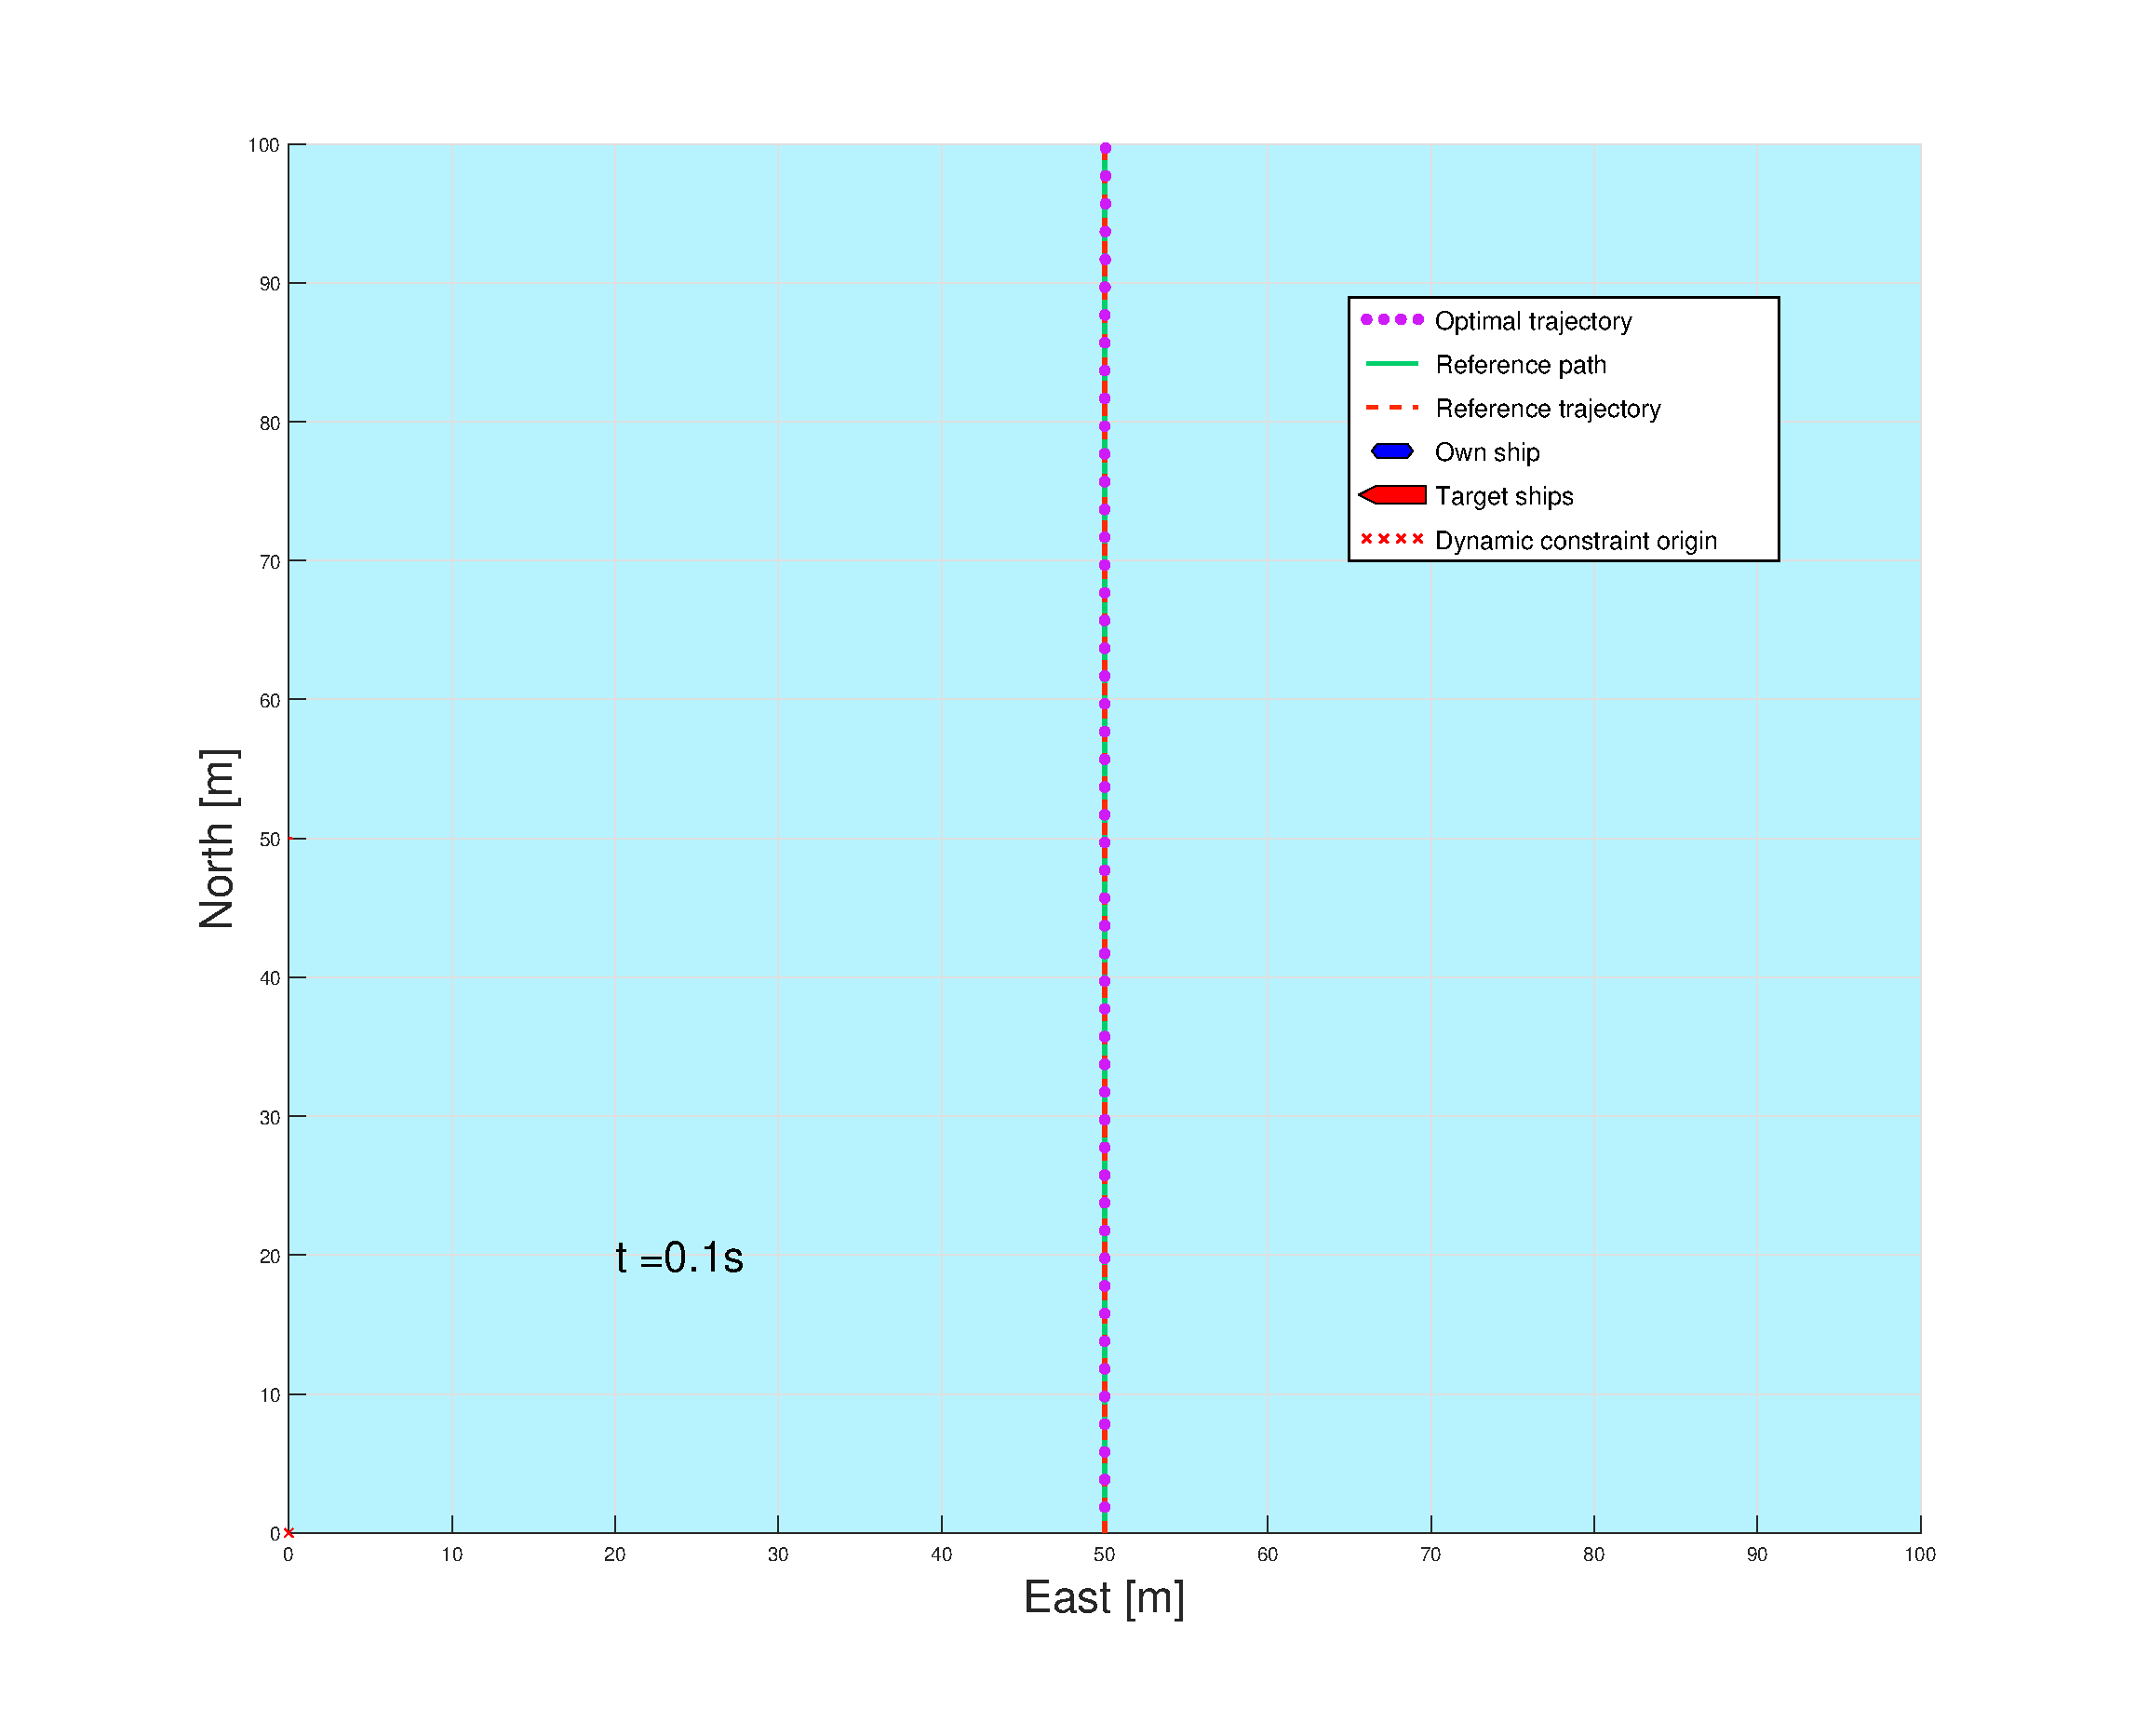
\includegraphics[width=\textwidth]{Images/Figures/enkel_SO/_Simple_0fig999_time=0}
    %     \subcaption{}
    % \end{subfigure}
    % \hfill
    % \\
    \begin{subfigure}[b]{0.49\textwidth}
        \centering
        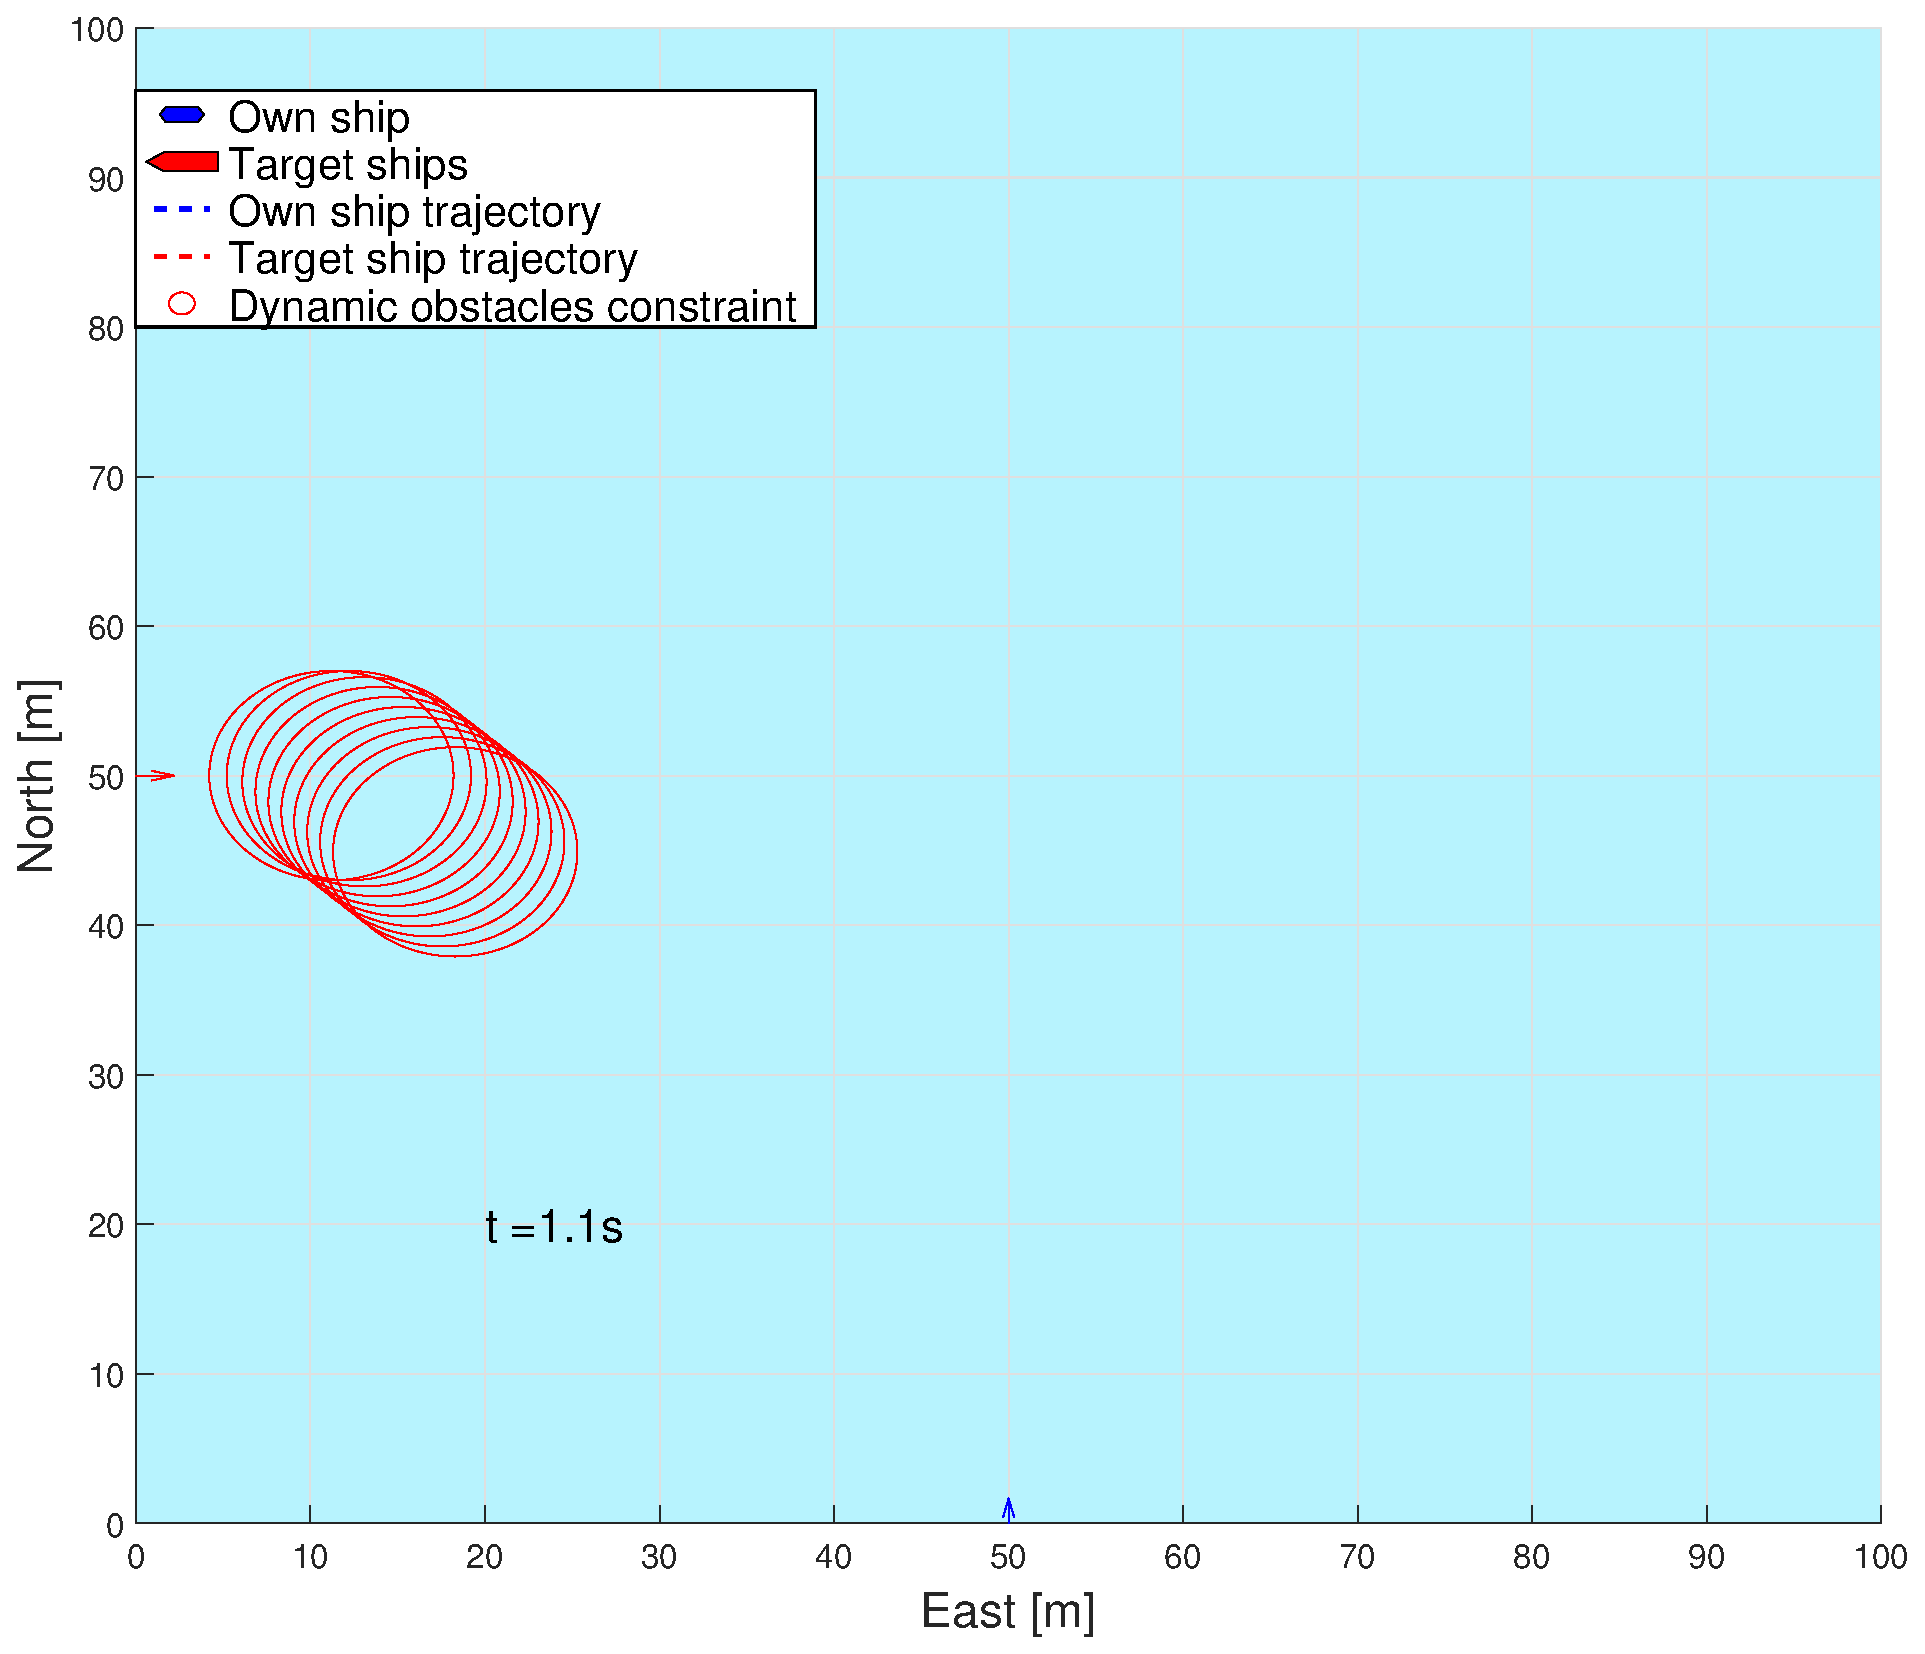
\includegraphics[width=\textwidth]{Images/Figures/enkel_SO/_Simple_0fig1_time=1}
        \subcaption{}
    \end{subfigure}
    \hfill
    \begin{subfigure}[b]{0.499\textwidth}
        \centering
        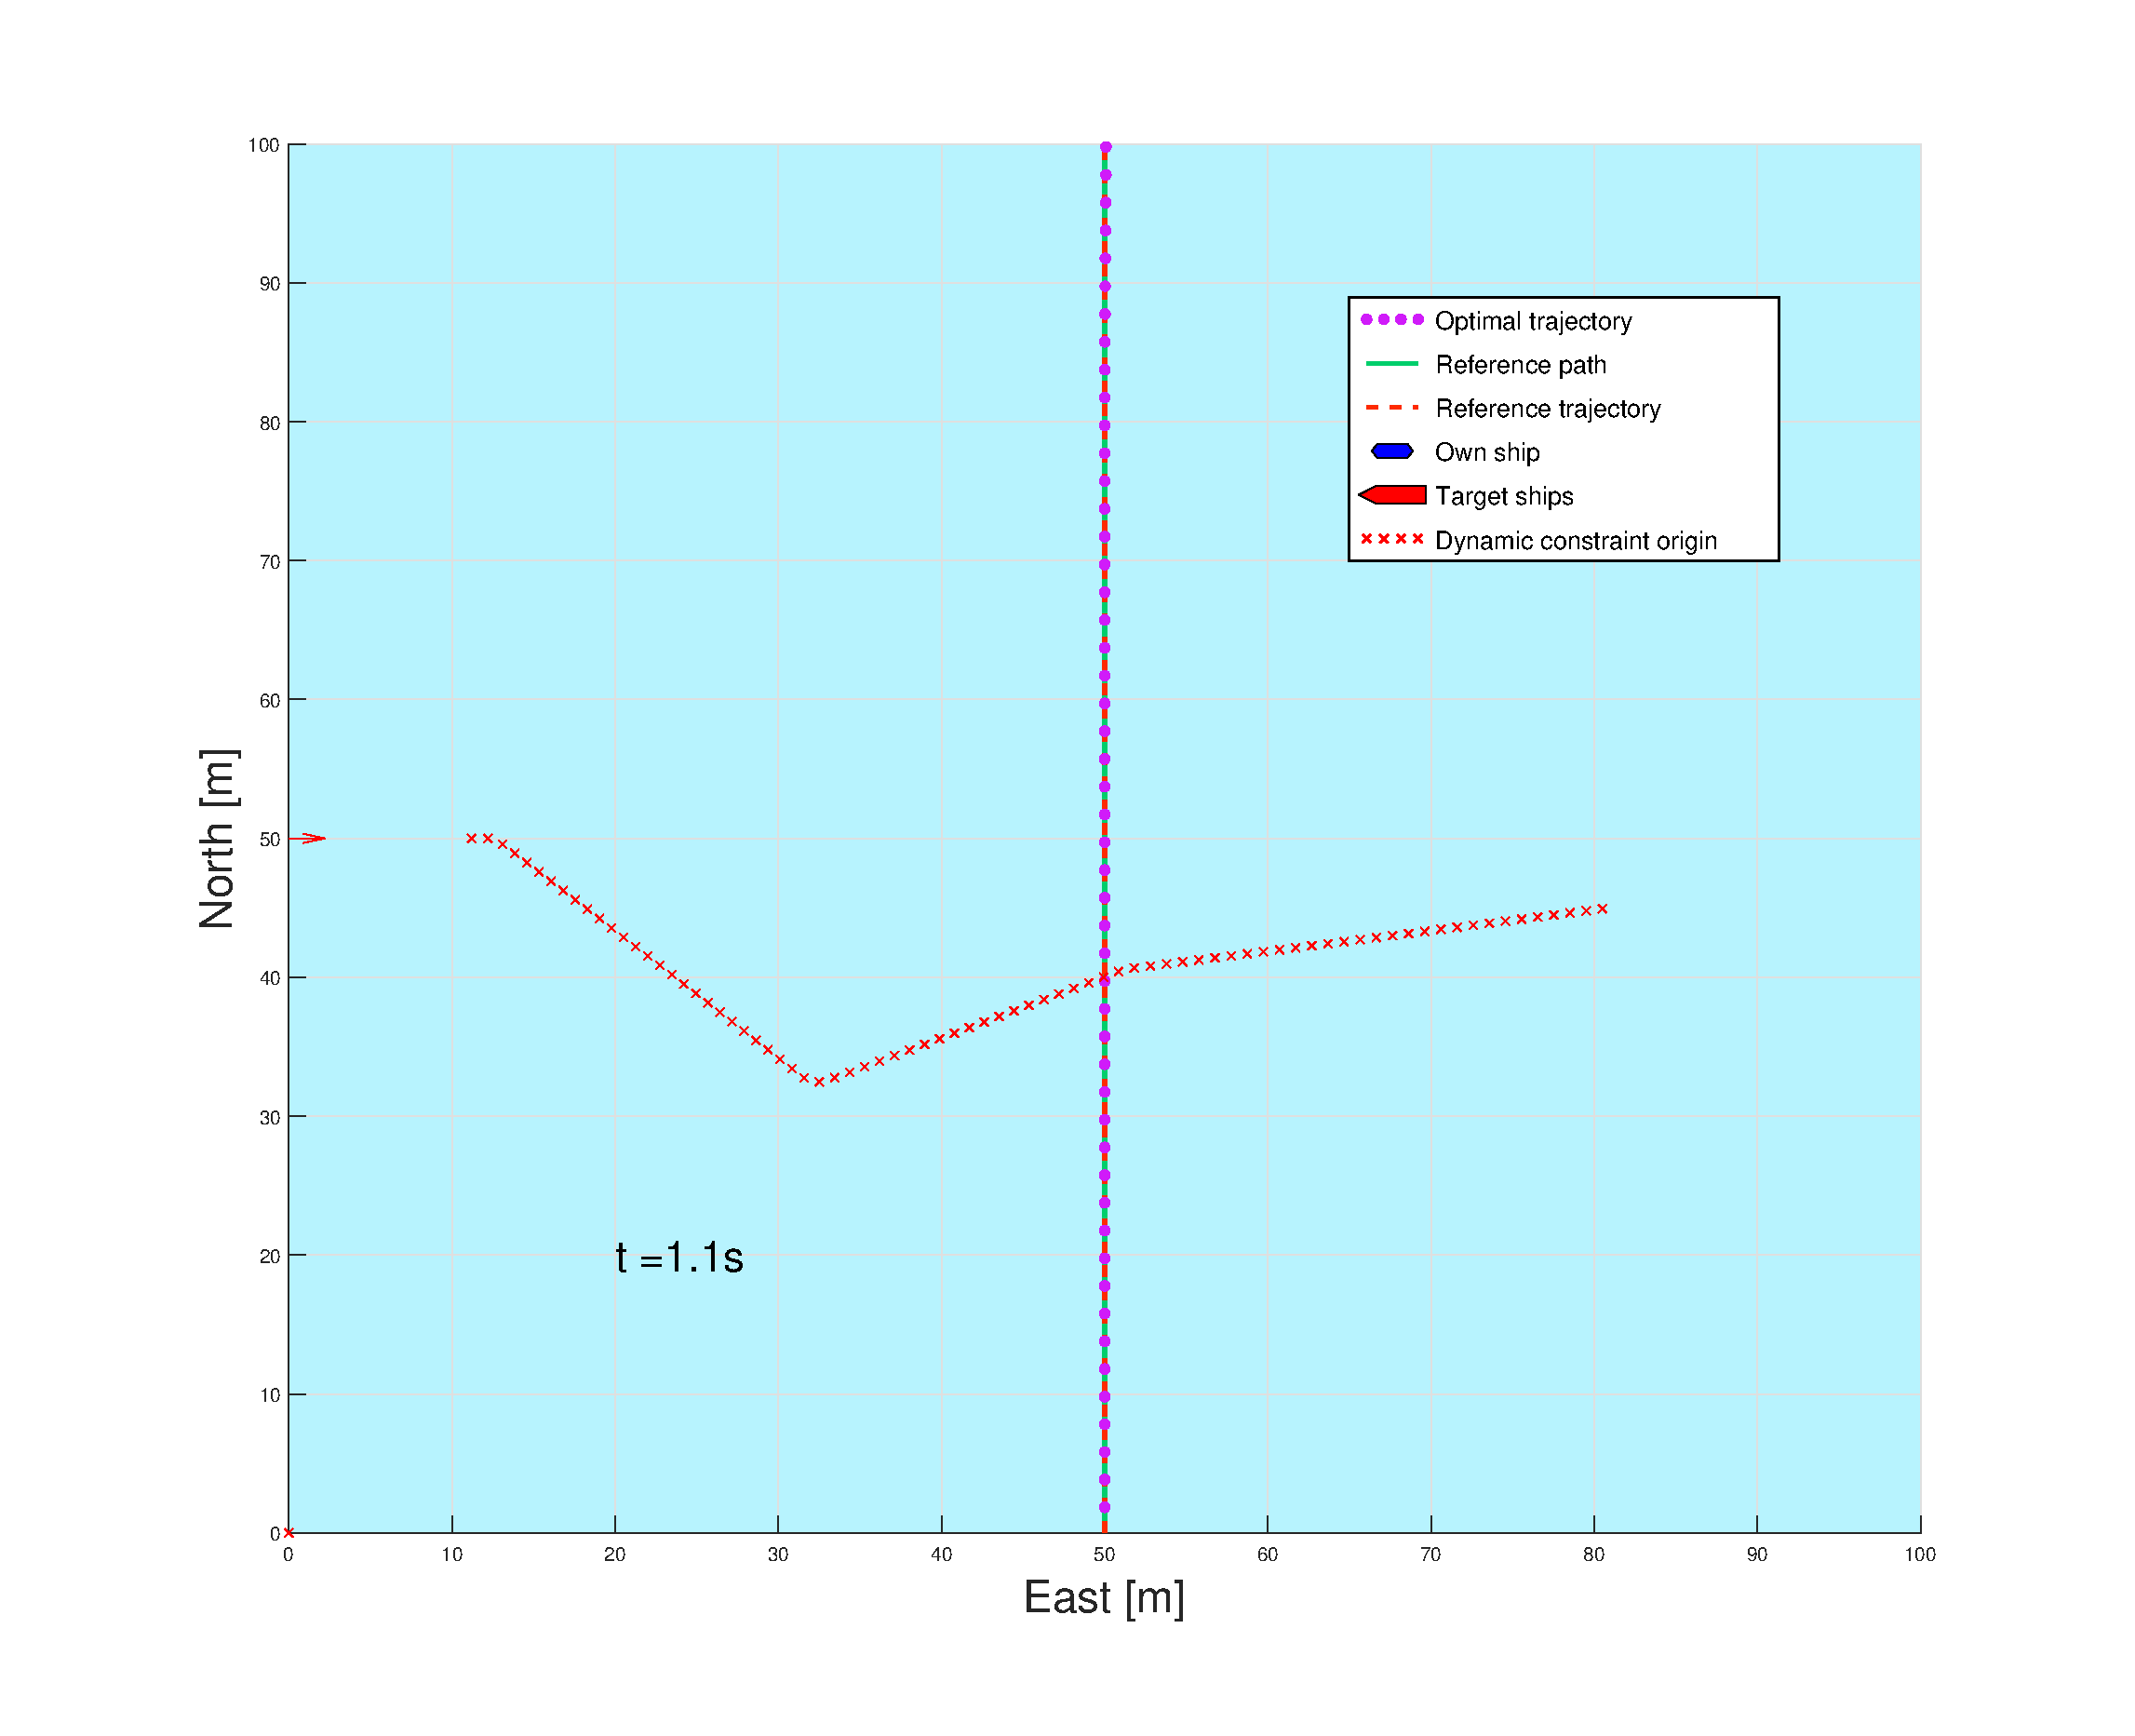
\includegraphics[width=\textwidth]{Images/Figures/enkel_SO/_Simple_0fig999_time=1}
        \subcaption{}
    \end{subfigure}
    \hfill
    \\
    \begin{subfigure}[b]{0.49\textwidth}
        \centering
        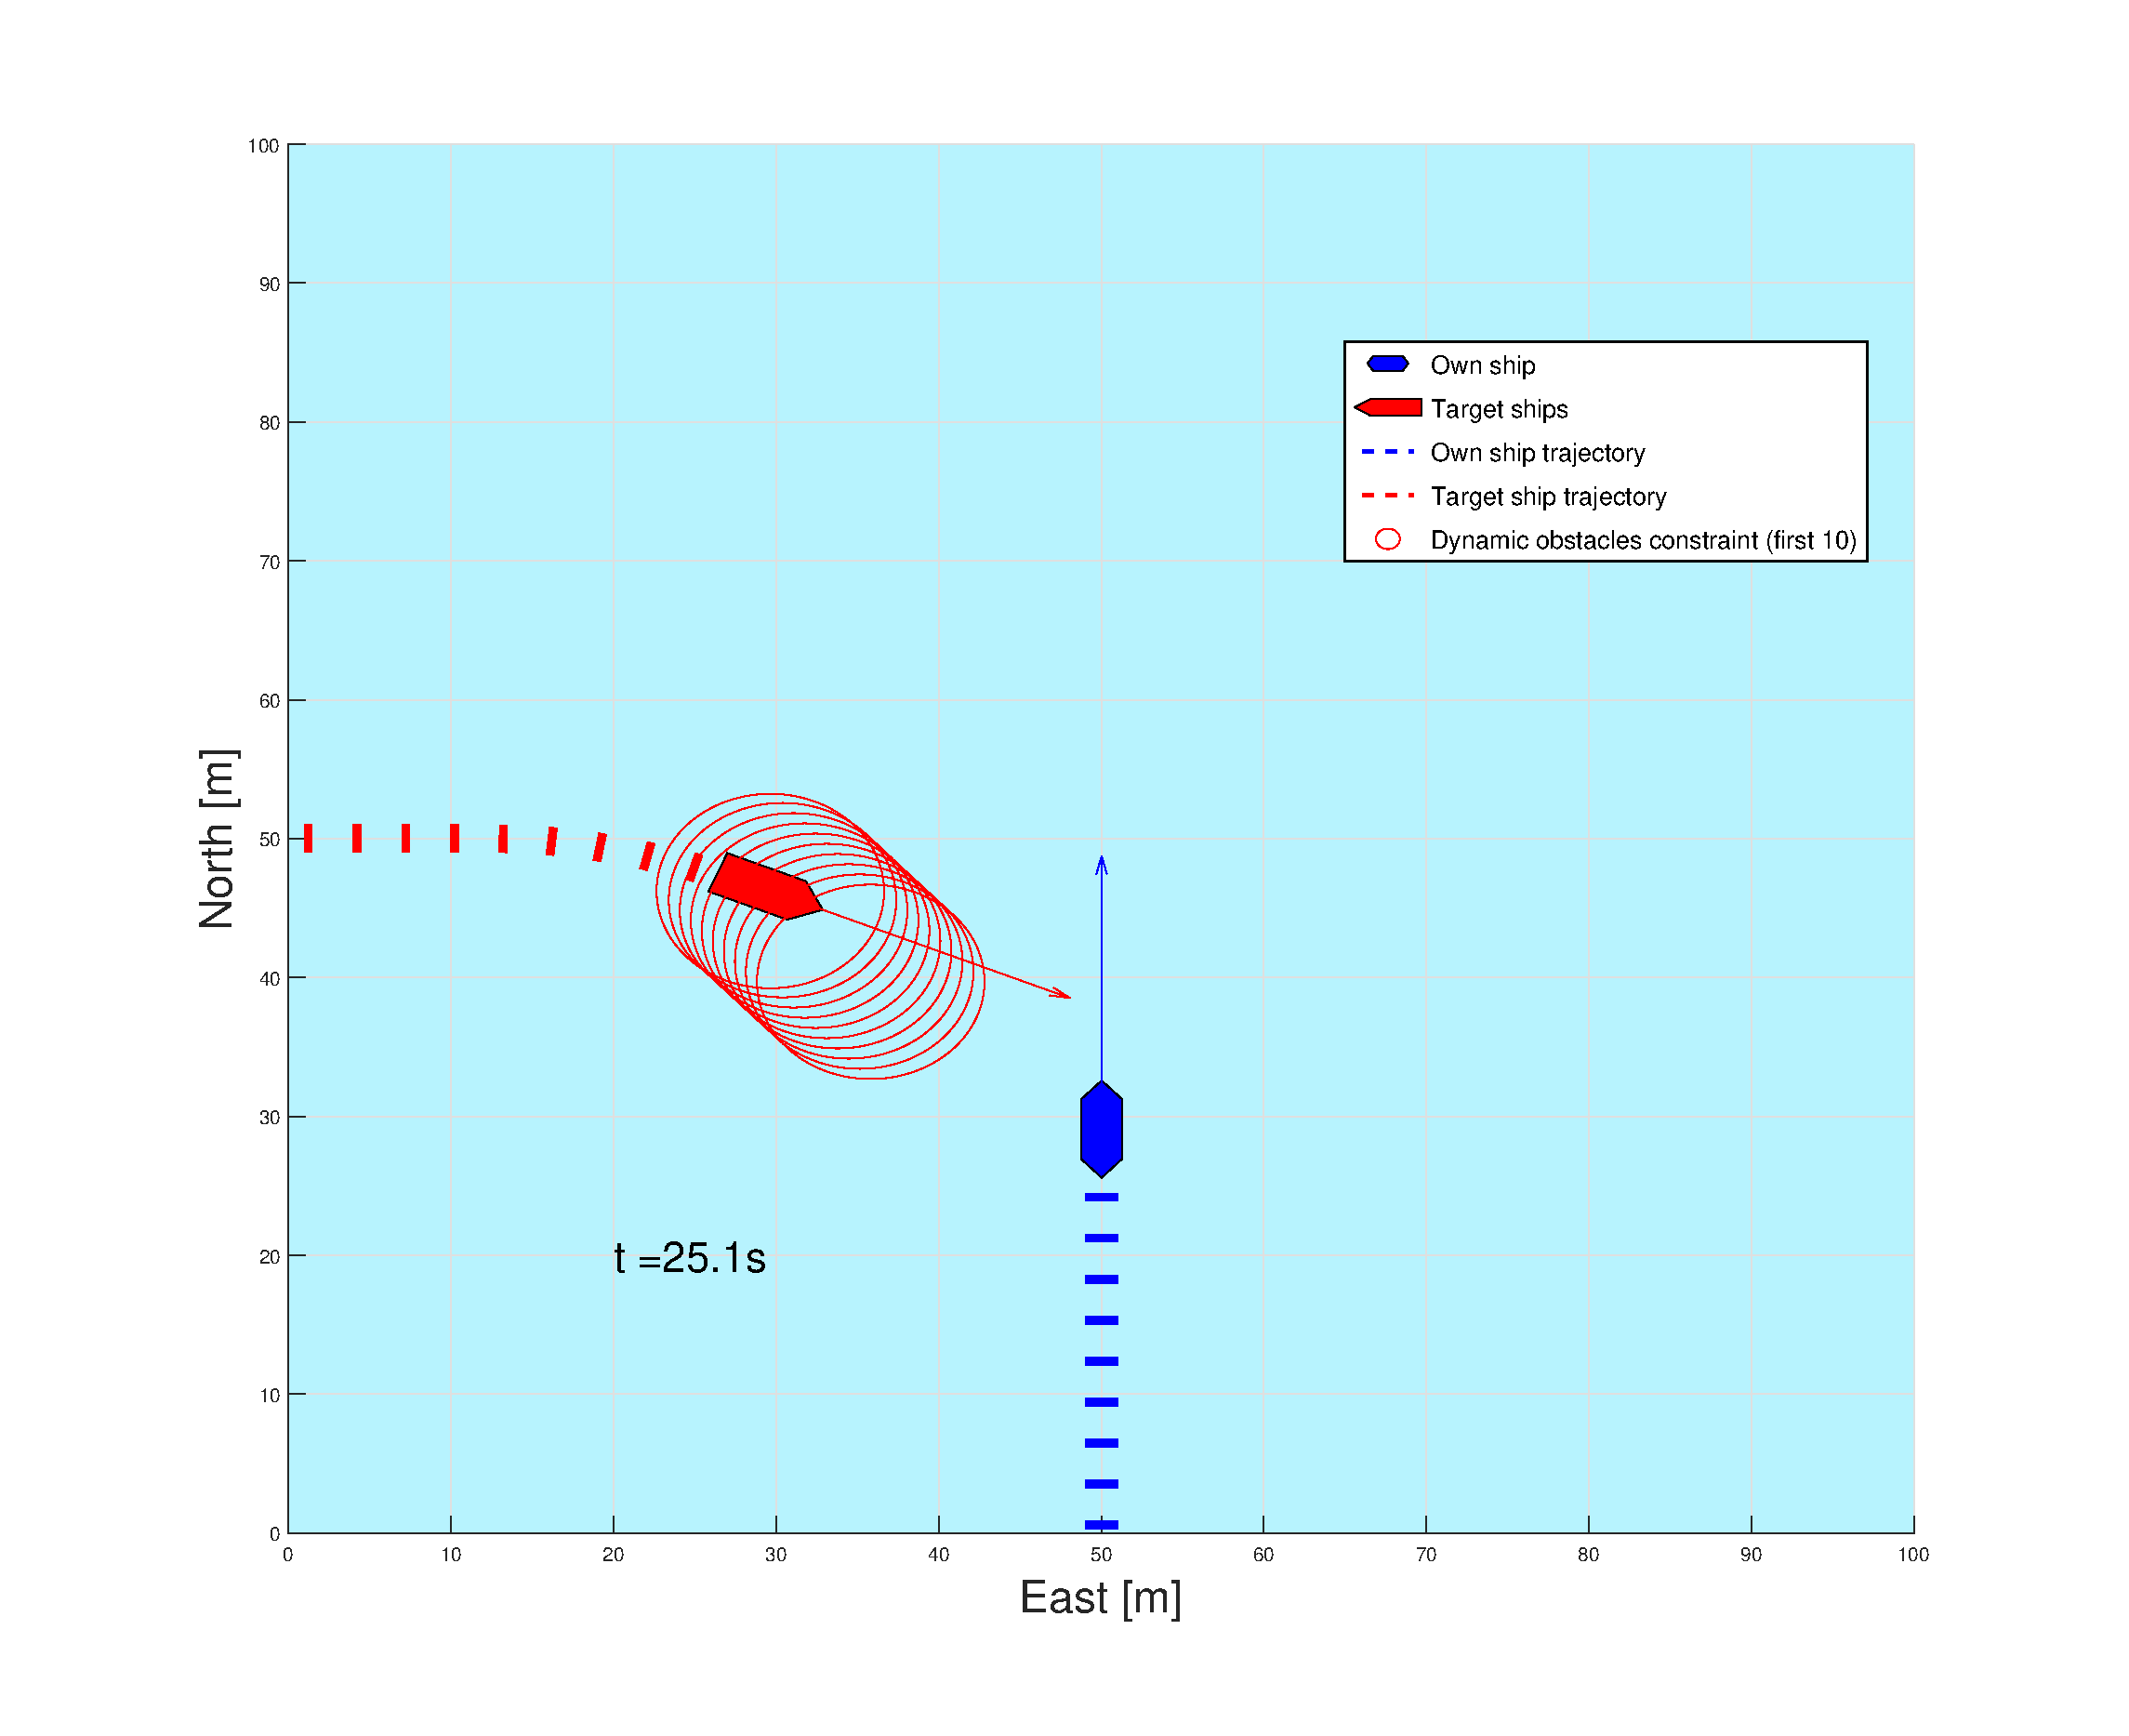
\includegraphics[width=\textwidth]{Images/Figures/enkel_SO/_Simple_0fig1_time=25}
        \subcaption{}
    \end{subfigure}
    \hfill
    \begin{subfigure}[b]{0.499\textwidth}
        \centering
        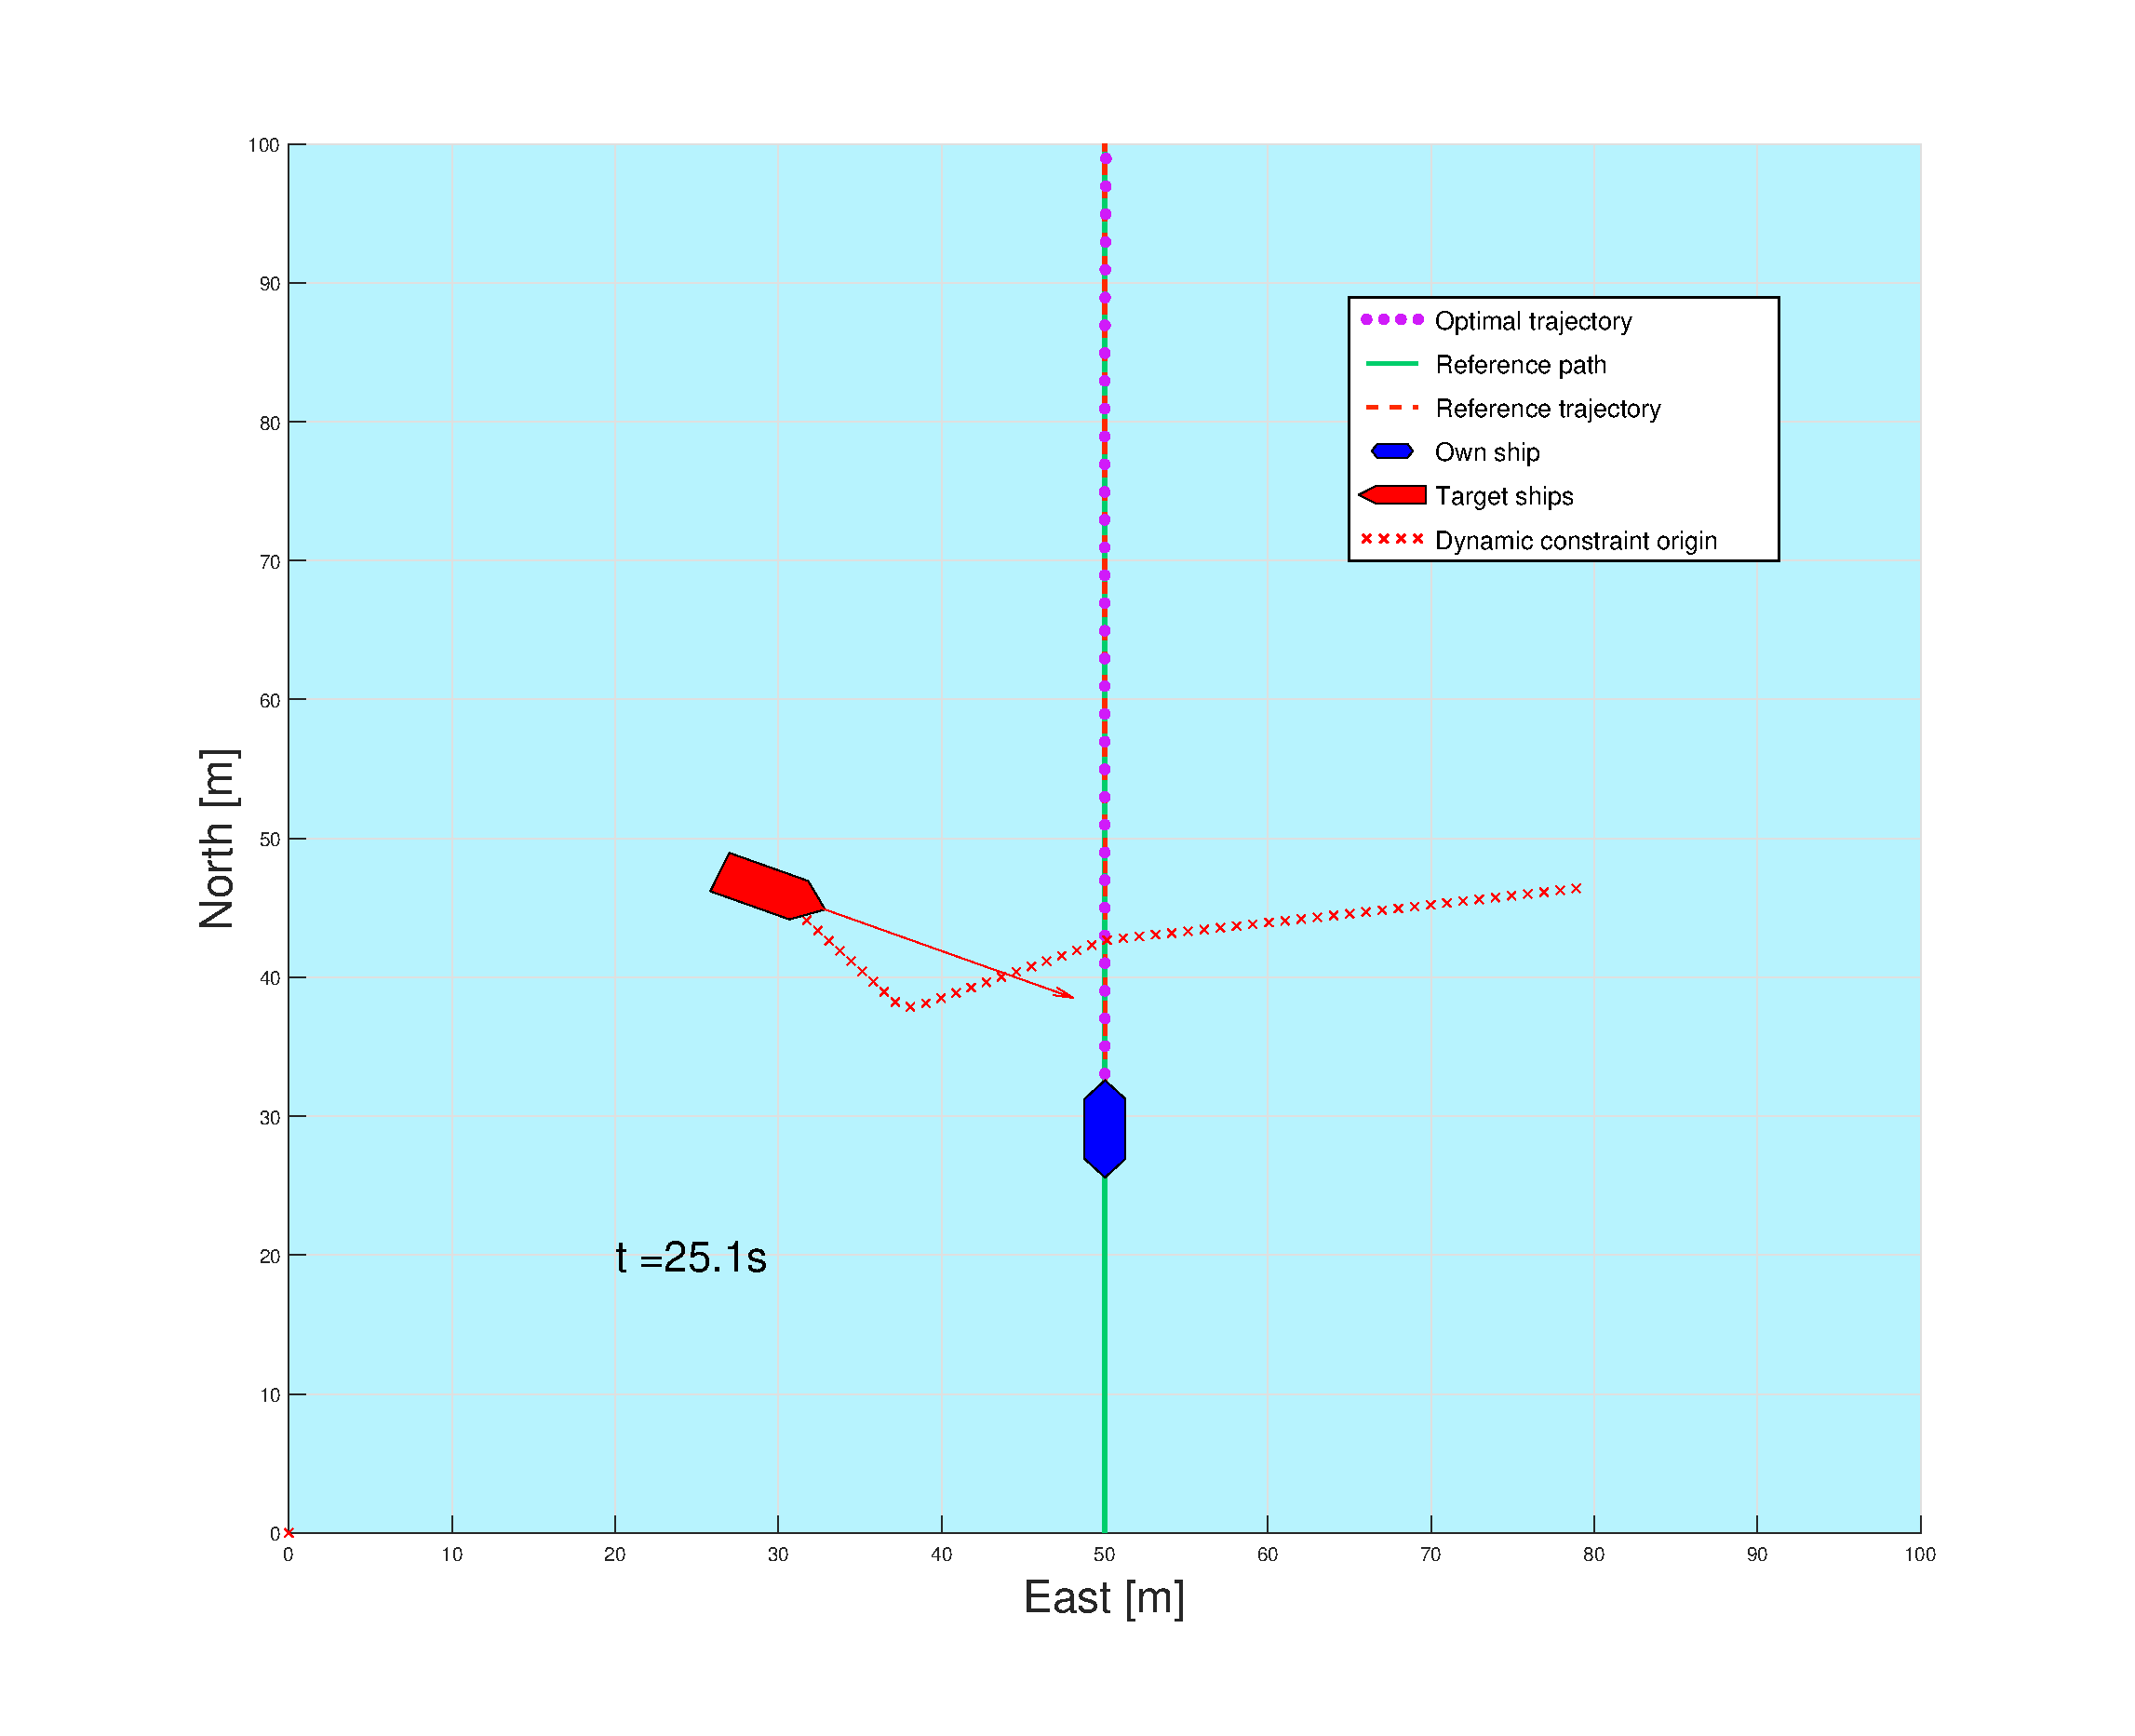
\includegraphics[width=\textwidth]{Images/Figures/enkel_SO/_Simple_0fig999_time=25}
        \subcaption{}
    \end{subfigure}
    \hfill
    \\
    \begin{subfigure}[b]{0.49\textwidth}
        \centering
        \includegraphics[width=\textwidth]{Images/Figures/enkel_SO/_Simple_0fig1_time=50}
        \subcaption{}
    \end{subfigure}
    \hfill
    \begin{subfigure}[b]{0.499\textwidth}
        \centering
        \includegraphics[width=\textwidth]{Images/Figures/enkel_SO/_Simple_0fig999_time=50}
        \subcaption{}
    \end{subfigure}
    \hfill
    \caption{Simple stand on situation. Here shown with full prediction, \gls{OS} correctly stands on.}
    \label{FIG: simple SO full pred}
\end{figure}%
% \begin{figure}[ht]\ContinuedFloat
%     \begin{subfigure}[b]{0.49\textwidth}
%         \centering
%         \includegraphics[width=\textwidth]{Images/Figures/enkel_SO/_Simple_0fig1_time=50}
%         \subcaption{}
%     \end{subfigure}
%     \hfill
%     \begin{subfigure}[b]{0.499\textwidth}
%         \centering
%         \includegraphics[width=\textwidth]{Images/Figures/enkel_SO/_Simple_0fig999_time=50}
%         \subcaption{}
%     \end{subfigure}
%     \hfill
%     \\
%     \begin{subfigure}[b]{0.49\textwidth}
%         \centering
%         \includegraphics[width=\textwidth]{Images/Figures/enkel_SO/_Simple_0fig1_time=75}
%         \subcaption{}
%     \end{subfigure}
%     \hfill
%     \begin{subfigure}[b]{0.499\textwidth}
%         \centering
%         \includegraphics[width=\textwidth]{Images/Figures/enkel_SO/_Simple_0fig999_time=75}
%         \subcaption{}
%     \end{subfigure}
%     \hfill
%     \caption{Simple Stand On With Prediction}
% \end{figure}

\begin{figure}[ht!] % Simple Stand on, without prediction.
    % \begin{subfigure}[b]{0.49\textwidth}
    %     \centering
    %     \includegraphics[width=\textwidth]{Images/Figures/enkel_SO/_Simple_1fig1_time=0}
    %     \subcaption{}
    % \end{subfigure}
    % \hfill
    % \begin{subfigure}[b]{0.499\textwidth}
    %     \centering
    %     \includegraphics[width=\textwidth]{Images/Figures/enkel_SO/_Simple_1fig999_time=0}
    %     \subcaption{}
    % \end{subfigure}
    % \hfill
    % \\
    \begin{subfigure}[b]{0.49\textwidth}
        \centering
        \includegraphics[width=\textwidth]{Images/Figures/enkel_SO/_Simple_1fig1_time=1}
        \subcaption{}
    \end{subfigure}
    \hfill
    \begin{subfigure}[b]{0.499\textwidth}
        \centering
        \includegraphics[width=\textwidth]{Images/Figures/enkel_SO/_Simple_1fig999_time=1}
        \subcaption{}
    \end{subfigure}
    \hfill
    \\
    \begin{subfigure}[b]{0.49\textwidth}
        \centering
        \includegraphics[width=\textwidth]{Images/Figures/enkel_SO/_Simple_1fig1_time=25}
        \subcaption{}
    \end{subfigure}
    \hfill
    \begin{subfigure}[b]{0.499\textwidth}
        \centering
        \includegraphics[width=\textwidth]{Images/Figures/enkel_SO/_Simple_1fig999_time=25}
        \subcaption{}
    \end{subfigure}
    \hfill
    \\
    \begin{subfigure}[b]{0.49\textwidth}
        \centering
        \includegraphics[width=\textwidth]{Images/Figures/enkel_SO/_Simple_1fig1_time=50}
        \subcaption{}
    \end{subfigure}
    \hfill
    \begin{subfigure}[b]{0.499\textwidth}
        \centering
        \includegraphics[width=\textwidth]{Images/Figures/enkel_SO/_Simple_1fig999_time=50}
        \subcaption{}
    \end{subfigure}
    \hfill
    \caption{Simple stand on situation. Here shown with simple prediction, the \gls{OS} can be observed to yield when it shouldn't.}
    \label{FIG: Simple SO simple pred}
\end{figure}%
% \begin{figure}[ht]\ContinuedFloat
%     \begin{subfigure}[b]{0.49\textwidth}
%         \centering
%         \includegraphics[width=\textwidth]{Images/Figures/enkel_SO/_Simple_1fig1_time=50}
%         \subcaption{}
%     \end{subfigure}
%     \hfill
%     \begin{subfigure}[b]{0.499\textwidth}
%         \centering
%         \includegraphics[width=\textwidth]{Images/Figures/enkel_SO/_Simple_1fig999_time=50}
%         \subcaption{}
%     \end{subfigure}
%     \hfill
%     \\
%     \begin{subfigure}[b]{0.49\textwidth}
%         \centering
%         \includegraphics[width=\textwidth]{Images/Figures/enkel_SO/_Simple_1fig1_time=75}
%         \subcaption{}
%     \end{subfigure}
%     \hfill
%     \begin{subfigure}[b]{0.499\textwidth}
%         \centering
%         \includegraphics[width=\textwidth]{Images/Figures/enkel_SO/_Simple_1fig999_time=75}
%         \subcaption{}
%     \end{subfigure}
%     \hfill
%     \caption{Simple Stand On Without Prediction}
% \end{figure}

\clearpage
\subsubsection{Simple Head On}
% \begin{itemize}
%     \item Very straight forward result, behaviour is exactly as one would expect given the placement of the constraint.
%     \item No difference between full and simple prediction because target ship holds steady course and velocity.
%     \item This is the behaviour we can expect every time a target ship is met directly head on and there are no other disturbances.
% \end{itemize}
The simple situations are not really meant to test anything, rather this scenario and the others are used for establishing
a baseline of capabilities. For example for this scenario specifically it is established that the OS will always attempt to
pass the head-on vessel on the port side when the conditions are ideal. This result holds for both simple and
full prediction levels. The result for this scenario is seen in Figure \ref{FIG: Simple HO}

\subsubsection{Simple Give Way}
% \begin{itemize}
%     \item It would be highly unusual to start using the trajectory planner when alredy this close to a situation
%     \item This is reflected in the strange behaviour where our path is completely blocked when dynamic obstacle constrains are enabled.
%     \item otherwise the behaviour ends up being exactly as expected considering the placements of the constraints.
% \end{itemize}
This scenario shows how the algorithm behaves when giving way to a crossing vessel. It might actually be a bit overzealous with this
constraint size, but that's something that can be tuned with further experimentation. One important observation to make from this
simple scenario is when obstacles are enabled on the second iteration of the algorithm, the constraints block the previous optimal
trajectory and causes it to be infeasible. This is more clearly observed in the video version. When the infeasibility is detected
the next result is a much shorter path as the speed is reduced, and then finally the full trajectory that gives way is found.
This very simple simulation highlights one of the potential problems with the algorithm, if it's turned on while the OS is in an active
COLREGs situation performance might be poor. The results are seen in Figure \ref{FIG: simple GW}

\subsubsection{Simple Stand On}
% \begin{itemize}
%     \item This scenario assumes that the \gls{Ts} plays nice and attempts to follow the \gls{COLREGs} rules.
%     \item When using simple prediction the optimal path is pushed towads port side behind the \gls{Ts}, and as the \gls{Ts} begins to turn the \gls{OS} is dragged along by the movement of the constraints.
%     \item This is actually quite unrealistic, there is no reason to assume the \gls{Ts} would continue to yield after observing the \gls{OS} change course like this. It's also a bad result for simple prediction because the behaviour can cause confusion\\
%     for other navigator.
%     \item The author realized late that the way prediction is done of the \gls{Ts} is not entirely consistent with the way prediction is handled internally in the algorithm. In the algorithm waypoints are used to predict \gls{Ts}s trajectories, which is not neccessary\\
%     the exact same trajectory as the \gls{Ts} ends up following. 
%     \item In order to get the \gls{Ts} to comply with expected \gls{COLREGs} behaviour a waypoint was placed some meters south of the \gls{OS} position at the would be \gls{tCPA}. This waypoint would obviously not exist in a normal transit situation and so\\
%     this scenario is actually a bit of a cheat in regards to how prediction is argued for in prior chapters.
%     \item The result is still interesting, for this scenario only we can exchange the advanced prediction result with a fully accurate prediction, and the result for simple prediction would hold for the current algorithm in all cases.
% \end{itemize}
This scenario is one of the two scenarios that assumes a cooperative TS, controlling the TSs to be cooperative turned out to be a real time sink, for longer scenarios
it simply wasn't worth the effort to include a TS that \textit{didn't} affect the OS.
This is also the first simulation where a difference between simple and full
prediction can be observed, and it's mostly the fault of poor constraint placement, which will be more thoroughly 
discussed in Chapter \ref{CHAP: discussion}. The full prediction result can be seen in
Figure \ref{FIG: simple SO full pred} and shows that the OS does not deviate from its speed or course, which is exactly the behavior we would want. 
The simple prediction version on the other hand, seen in Figure \ref{FIG: Simple SO simple pred} turns to cross behind the incoming TS.

\clearpage
\begin{figure}[ht!] % TURN HEAD ON WITH PREDICTION
    % \begin{subfigure}[b]{0.49\textwidth}
    %     \centering
    %     \includegraphics[width=\textwidth]{Images/Figures/sving_HO/_Simple_0fig1_time=1}
    %     \subcaption{}
    % \end{subfigure}
    % \hfill
    % \begin{subfigure}[b]{0.499\textwidth}
    %     \centering
    %     \includegraphics[width=\textwidth]{Images/Figures/sving_HO/_Simple_0fig999_time=1}
    %     \subcaption{}
    % \end{subfigure}
    % \hfill
    % \\
    \begin{subfigure}[b]{0.494\textwidth}
        \centering
        \includegraphics[width=\textwidth]{Images/Figures/sving_HO/_Simple_0fig1_time=25}
        \subcaption{}
    \end{subfigure}
    \hfill
    \begin{subfigure}[b]{0.494\textwidth}
        \centering
        \includegraphics[width=\textwidth]{Images/Figures/sving_HO/_Simple_0fig999_time=25}
        \subcaption{}
    \end{subfigure}
    \hfill
    \\
    \begin{subfigure}[b]{0.494\textwidth}
        \centering
        \includegraphics[width=\textwidth]{Images/Figures/sving_HO/_Simple_0fig1_time=50}
        \subcaption{}
    \end{subfigure}
    \hfill
    \begin{subfigure}[b]{0.494\textwidth}
        \centering
        \includegraphics[width=\textwidth]{Images/Figures/sving_HO/_Simple_0fig999_time=50}
        \subcaption{}
    \end{subfigure}
    \hfill
    \\
    \begin{subfigure}[b]{0.494\textwidth}
        \centering
        \includegraphics[width=\textwidth]{Images/Figures/sving_HO/_Simple_0fig1_time=75}
        \subcaption{}
    \end{subfigure}
    \hfill
    \begin{subfigure}[b]{0.494\textwidth}
        \centering
        \includegraphics[width=\textwidth]{Images/Figures/sving_HO/_Simple_0fig999_time=75}
        \subcaption{}
    \end{subfigure}
    \hfill
    \caption{Head on situation with a turn, Result for this were the same regardless of prediction level.}
    \label{FIG: Turn HO}
\end{figure}%
% \begin{figure}[ht]\ContinuedFloat
%     \begin{subfigure}[b]{0.49\textwidth}
%         \centering
%         \includegraphics[width=\textwidth]{Images/Figures/sving_HO/_Simple_0fig1_time=75}
%         \subcaption{}
%     \end{subfigure}
%     \hfill
%     \begin{subfigure}[b]{0.499\textwidth}
%         \centering
%         \includegraphics[width=\textwidth]{Images/Figures/sving_HO/_Simple_0fig999_time=75}
%         \subcaption{}
%     \end{subfigure}
%     \hfill
%     \\
%     \begin{subfigure}[b]{0.49\textwidth}
%         \centering
%         \includegraphics[width=\textwidth]{Images/Figures/sving_HO/_Simple_0fig1_time=101}
%         \subcaption{}
%     \end{subfigure}
%     \hfill
%     \begin{subfigure}[b]{0.499\textwidth}
%         \centering
%         \includegraphics[width=\textwidth]{Images/Figures/sving_HO/_Simple_0fig999_time=101}
%         \subcaption{}
%     \end{subfigure}
%     \hfill
%     \caption{Turn Head On With Prediction}
% \end{figure}

% \begin{figure}[!b] % TURN HEAD ON WITHOUT PREDICTION
%     \begin{subfigure}[b]{0.49\textwidth}
%         \centering
%         \includegraphics[width=\textwidth]{Images/Figures/sving_HO/_Simple_1fig1_time=1}
%         \subcaption{}
%     \end{subfigure}
%     \hfill
%     \begin{subfigure}[b]{0.499\textwidth}
%         \centering
%         \includegraphics[width=\textwidth]{Images/Figures/sving_HO/_Simple_1fig999_time=1}
%         \subcaption{}
%     \end{subfigure}
%     \hfill
%     \\
%     \begin{subfigure}[b]{0.49\textwidth}
%         \centering
%         \includegraphics[width=\textwidth]{Images/Figures/sving_HO/_Simple_1fig1_time=25}
%         \subcaption{}
%     \end{subfigure}
%     \hfill
%     \begin{subfigure}[b]{0.499\textwidth}
%         \centering
%         \includegraphics[width=\textwidth]{Images/Figures/sving_HO/_Simple_1fig999_time=25}
%         \subcaption{}
%     \end{subfigure}
%     \hfill
%     \\
%     \begin{subfigure}[b]{0.49\textwidth}
%         \centering
%         \includegraphics[width=\textwidth]{Images/Figures/sving_HO/_Simple_1fig1_time=50}
%         \subcaption{}
%     \end{subfigure}
%     \hfill
%     \begin{subfigure}[b]{0.499\textwidth}
%         \centering
%         \includegraphics[width=\textwidth]{Images/Figures/sving_HO/_Simple_1fig999_time=50}
%         \subcaption{}
%     \end{subfigure}
%     \hfill
% \end{figure}%
% \begin{figure}[ht]\ContinuedFloat
%     \begin{subfigure}[b]{0.49\textwidth}
%         \centering
%         \includegraphics[width=\textwidth]{Images/Figures/sving_HO/_Simple_1fig1_time=75}
%         \subcaption{}
%     \end{subfigure}
%     \hfill
%     \begin{subfigure}[b]{0.499\textwidth}
%         \centering
%         \includegraphics[width=\textwidth]{Images/Figures/sving_HO/_Simple_1fig999_time=75}
%         \subcaption{}
%     \end{subfigure}
%     \hfill
%     \\
%     \begin{subfigure}[b]{0.49\textwidth}
%         \centering
%         \includegraphics[width=\textwidth]{Images/Figures/sving_HO/_Simple_1fig1_time=101}
%         \subcaption{}
%     \end{subfigure}
%     \hfill
%     \begin{subfigure}[b]{0.499\textwidth}
%         \centering
%         \includegraphics[width=\textwidth]{Images/Figures/sving_HO/_Simple_1fig999_time=101}
%         \subcaption{}
%     \end{subfigure}
%     \hfill
%     \caption{Turn Head On WithOUT Prediction}
% \end{figure}

\begin{figure}[ht!] % TURN GIVE WAY WITH PREDICTION
    % \begin{subfigure}[b]{0.49\textwidth}
    %     \centering
    %     \includegraphics[width=\textwidth]{Images/Figures/sving_GW/_Simple_0fig1_time=1}
    %     \subcaption{}
    % \end{subfigure}
    % \hfill
    % \begin{subfigure}[b]{0.499\textwidth}
    %     \centering
    %     \includegraphics[width=\textwidth]{Images/Figures/sving_GW/_Simple_0fig999_time=1}
    %     \subcaption{}
    % \end{subfigure}
    % \hfill
    % \\
    \begin{subfigure}[b]{0.494\textwidth}
        \centering
        \includegraphics[width=\textwidth]{Images/Figures/sving_GW/_Simple_0fig1_time=25}
        \subcaption{}
    \end{subfigure}
    \hfill
    \begin{subfigure}[b]{0.494\textwidth}
        \centering
        \includegraphics[width=\textwidth]{Images/Figures/sving_GW/_Simple_0fig999_time=25}
        \subcaption{}
    \end{subfigure}
    \hfill
    \\
    \begin{subfigure}[b]{0.494\textwidth}
        \centering
        \includegraphics[width=\textwidth]{Images/Figures/sving_GW/_Simple_0fig1_time=50}
        \subcaption{}
    \end{subfigure}
    \hfill
    \begin{subfigure}[b]{0.494\textwidth}
        \centering
        \includegraphics[width=\textwidth]{Images/Figures/sving_GW/_Simple_0fig999_time=50}
        \subcaption{}
    \end{subfigure}
    \hfill
    \\
    \begin{subfigure}[b]{0.494\textwidth}
        \centering
        \includegraphics[width=\textwidth]{Images/Figures/sving_GW/_Simple_0fig1_time=75}
        \subcaption{}
    \end{subfigure}
    \hfill
    \begin{subfigure}[b]{0.494\textwidth}
        \centering
        \includegraphics[width=\textwidth]{Images/Figures/sving_GW/_Simple_0fig999_time=75}
        \subcaption{}
    \end{subfigure}
    \hfill
    \caption{Give way with a turn, here with full prediction. Observe the \gls{OS} not execting to have to yield until it's almost too late.}
    \label{FIG: turn GW full pred}
\end{figure}%
% \begin{figure}[ht]\ContinuedFloat
%     \begin{subfigure}[b]{0.49\textwidth}
%         \centering
%         \includegraphics[width=\textwidth]{Images/Figures/sving_GW/_Simple_0fig1_time=75}
%         \subcaption{}
%     \end{subfigure}
%     \hfill
%     \begin{subfigure}[b]{0.499\textwidth}
%         \centering
%         \includegraphics[width=\textwidth]{Images/Figures/sving_GW/_Simple_0fig999_time=75}
%         \subcaption{}
%     \end{subfigure}
%     \hfill
%     \\
%     \begin{subfigure}[b]{0.49\textwidth}
%         \centering
%         \includegraphics[width=\textwidth]{Images/Figures/sving_GW/_Simple_0fig1_time=101}
%         \subcaption{}
%     \end{subfigure}
%     \hfill
%     \begin{subfigure}[b]{0.499\textwidth}
%         \centering
%         \includegraphics[width=\textwidth]{Images/Figures/sving_GW/_Simple_0fig999_time=101}
%         \subcaption{}
%     \end{subfigure}
%     \hfill
%     \caption{Turn GIVE WAY With Prediction}
% \end{figure}

\begin{figure}[ht!] % TURN GIVE WAY WITHOUT PREDICTION
    % \begin{subfigure}[b]{0.49\textwidth}
    %     \centering
    %     \includegraphics[width=\textwidth]{Images/Figures/sving_GW/_Simple_0fig1_time=1}
    %     \subcaption{}
    % \end{subfigure}
    % \hfill
    % \begin{subfigure}[b]{0.499\textwidth}
    %     \centering
    %     \includegraphics[width=\textwidth]{Images/Figures/sving_GW/_Simple_0fig999_time=1}
    %     \subcaption{}
    % \end{subfigure}
    % \hfill
    % \\
    \begin{subfigure}[b]{0.494\textwidth}
        \centering
        \includegraphics[width=\textwidth]{Images/Figures/sving_GW/_Simple_1fig1_time=25}
        \subcaption{}
    \end{subfigure}
    \hfill
    \begin{subfigure}[b]{0.494\textwidth}
        \centering
        \includegraphics[width=\textwidth]{Images/Figures/sving_GW/_Simple_1fig999_time=25}
        \subcaption{}
    \end{subfigure}
    \hfill
    \\
    \begin{subfigure}[b]{0.494\textwidth}
        \centering
        \includegraphics[width=\textwidth]{Images/Figures/sving_GW/_Simple_1fig1_time=50}
        \subcaption{}
    \end{subfigure}
    \hfill
    \begin{subfigure}[b]{0.494\textwidth}
        \centering
        \includegraphics[width=\textwidth]{Images/Figures/sving_GW/_Simple_1fig999_time=50}
        \subcaption{}
    \end{subfigure}
    \hfill
    \\
    \begin{subfigure}[b]{0.494\textwidth}
        \centering
        \includegraphics[width=\textwidth]{Images/Figures/sving_GW/_Simple_1fig1_time=75}
        \subcaption{}
    \end{subfigure}
    \hfill
    \begin{subfigure}[b]{0.494\textwidth}
        \centering
        \includegraphics[width=\textwidth]{Images/Figures/sving_GW/_Simple_1fig999_time=75}
        \subcaption{}
    \end{subfigure}
    \hfill
    \caption{Give way with a turn, here with simple prediction. Observe as the OS gets dragged along by the constraints of the turning TS.}
    \label{FIG: turn GW simple pred}
\end{figure}%
% \begin{figure}[ht]\ContinuedFloat
%     \begin{subfigure}[b]{0.49\textwidth}
%         \centering
%         \includegraphics[width=\textwidth]{Images/Figures/sving_GW/_Simple_1fig1_time=75}
%         \subcaption{}
%     \end{subfigure}
%     \hfill
%     \begin{subfigure}[b]{0.499\textwidth}
%         \centering
%         \includegraphics[width=\textwidth]{Images/Figures/sving_GW/_Simple_1fig999_time=75}
%         \subcaption{}
%     \end{subfigure}
%     \hfill
%     \\
%     \begin{subfigure}[b]{0.49\textwidth}
%         \centering
%         \includegraphics[width=\textwidth]{Images/Figures/sving_GW/_Simple_1fig1_time=101}
%         \subcaption{}
%     \end{subfigure}
%     \hfill
%     \begin{subfigure}[b]{0.499\textwidth}
%         \centering
%         \includegraphics[width=\textwidth]{Images/Figures/sving_GW/_Simple_1fig999_time=101}
%         \subcaption{}
%     \end{subfigure}
%     \hfill
%     \caption{Turn GIVE WAY WithOUT Prediction}
% \end{figure}

\begin{figure}[ht!] % TURN STAND ON WITH PREDICTION
    % \begin{subfigure}[b]{0.49\textwidth}
    %     \centering
    %     \includegraphics[width=\textwidth]{Images/Figures/sving_SO/_Simple_0fig1_time=1}
    %     \subcaption{}
    % \end{subfigure}
    % \hfill
    % \begin{subfigure}[b]{0.499\textwidth}
    %     \centering
    %     \includegraphics[width=\textwidth]{Images/Figures/sving_SO/_Simple_0fig999_time=1}
    %     \subcaption{}
    % \end{subfigure}
    % \hfill
    % \\
    \begin{subfigure}[b]{0.494\textwidth}
        \centering
        \includegraphics[width=\textwidth]{Images/Figures/sving_SO/_Simple_0fig1_time=25}
        \subcaption{}
    \end{subfigure}
    \hfill
    \begin{subfigure}[b]{0.494\textwidth}
        \centering
        \includegraphics[width=\textwidth]{Images/Figures/sving_SO/_Simple_0fig999_time=25}
        \subcaption{}
    \end{subfigure}
    \hfill
    \\
    \begin{subfigure}[b]{0.494\textwidth}
        \centering
        \includegraphics[width=\textwidth]{Images/Figures/sving_SO/_Simple_0fig1_time=50}
        \subcaption{}
    \end{subfigure}
    \hfill
    \begin{subfigure}[b]{0.494\textwidth}
        \centering
        \includegraphics[width=\textwidth]{Images/Figures/sving_SO/_Simple_0fig999_time=50}
        \subcaption{}
    \end{subfigure}
    \hfill
    \\
    \begin{subfigure}[b]{0.494\textwidth}
        \centering
        \includegraphics[width=\textwidth]{Images/Figures/sving_SO/_Simple_0fig1_time=75}
        \subcaption{}
    \end{subfigure}
    \hfill
    \begin{subfigure}[b]{0.494\textwidth}
        \centering
        \includegraphics[width=\textwidth]{Images/Figures/sving_SO/_Simple_0fig999_time=75}
        \subcaption{}
    \end{subfigure}
    \hfill
    \caption{Stand on situation with turn. Result independent of prediction level.}
    \label{FIG: turn SO}
\end{figure}%
% \begin{figure}[ht]\ContinuedFloat
%     \begin{subfigure}[b]{0.49\textwidth}
%         \centering
%         \includegraphics[width=\textwidth]{Images/Figures/sving_SO/_Simple_0fig1_time=75}
%         \subcaption{}
%     \end{subfigure}
%     \hfill
%     \begin{subfigure}[b]{0.499\textwidth}
%         \centering
%         \includegraphics[width=\textwidth]{Images/Figures/sving_SO/_Simple_0fig999_time=75}
%         \subcaption{}
%     \end{subfigure}
%     \hfill
%     \\
%     \begin{subfigure}[b]{0.49\textwidth}
%         \centering
%         \includegraphics[width=\textwidth]{Images/Figures/sving_SO/_Simple_0fig1_time=101}
%         \subcaption{}
%     \end{subfigure}
%     \hfill
%     \begin{subfigure}[b]{0.499\textwidth}
%         \centering
%         \includegraphics[width=\textwidth]{Images/Figures/sving_SO/_Simple_0fig999_time=101}
%         \subcaption{}
%     \end{subfigure}
%     \hfill
%     \caption{Turn Stand On With Prediction}
% \end{figure}

% \begin{figure}[!b] % TURN STAND ON WITHOUT PREDICTION
%     \begin{subfigure}[b]{0.49\textwidth}
%         \centering
%         \includegraphics[width=\textwidth]{Images/Figures/sving_SO/_Simple_1fig1_time=1}
%         \subcaption{}
%     \end{subfigure}
%     \hfill
%     \begin{subfigure}[b]{0.499\textwidth}
%         \centering
%         \includegraphics[width=\textwidth]{Images/Figures/sving_SO/_Simple_1fig999_time=1}
%         \subcaption{}
%     \end{subfigure}
%     \hfill
%     \\
%     \begin{subfigure}[b]{0.49\textwidth}
%         \centering
%         \includegraphics[width=\textwidth]{Images/Figures/sving_SO/_Simple_1fig1_time=25}
%         \subcaption{}
%     \end{subfigure}
%     \hfill
%     \begin{subfigure}[b]{0.499\textwidth}
%         \centering
%         \includegraphics[width=\textwidth]{Images/Figures/sving_SO/_Simple_1fig999_time=25}
%         \subcaption{}
%     \end{subfigure}
%     \hfill
%     \\
%     \begin{subfigure}[b]{0.49\textwidth}
%         \centering
%         \includegraphics[width=\textwidth]{Images/Figures/sving_SO/_Simple_1fig1_time=50}
%         \subcaption{}
%     \end{subfigure}
%     \hfill
%     \begin{subfigure}[b]{0.499\textwidth}
%         \centering
%         \includegraphics[width=\textwidth]{Images/Figures/sving_SO/_Simple_1fig999_time=50}
%         \subcaption{}
%     \end{subfigure}
%     \hfill
% \end{figure}%
% \begin{figure}[ht]\ContinuedFloat
%     \begin{subfigure}[b]{0.49\textwidth}
%         \centering
%         \includegraphics[width=\textwidth]{Images/Figures/sving_SO/_Simple_1fig1_time=75}
%         \subcaption{}
%     \end{subfigure}
%     \hfill
%     \begin{subfigure}[b]{0.499\textwidth}
%         \centering
%         \includegraphics[width=\textwidth]{Images/Figures/sving_SO/_Simple_1fig999_time=75}
%         \subcaption{}
%     \end{subfigure}
%     \hfill
%     \\
%     \begin{subfigure}[b]{0.49\textwidth}
%         \centering
%         \includegraphics[width=\textwidth]{Images/Figures/sving_SO/_Simple_1fig1_time=101}
%         \subcaption{}
%     \end{subfigure}
%     \hfill
%     \begin{subfigure}[b]{0.499\textwidth}
%         \centering
%         \includegraphics[width=\textwidth]{Images/Figures/sving_SO/_Simple_1fig999_time=101}
%         \subcaption{}
%     \end{subfigure}
%     \hfill
%     \caption{Turn Stand On WithOUT Prediction}
% \end{figure}

\clearpage
\subsubsection{Turn Head On}
% \begin{itemize}
%     \item business as usual, an easy situation to maneuver through.
% \end{itemize}
Very similar result to the straight path head on situation, which is not entirely unexpected. One aspect of this scenario that
has become very obvious with hindsight is that the incoming TS should have approached from northwest instead of northeast. That way
any a poorly calculated optimal trajectory would have been dragged towards the wrong side for the crossing. Instead, as the situation is set
up the trajectory will always be pushed towards crossing on the correct side. (TODO: kanskje forklar dette bedre?).
The results for this scenario are seen in Figure \ref{FIG: Turn HO}

\subsubsection{Turn Give Way}
% \begin{itemize}
%     \item Here we finally observe a big differene between full and simple prediction.
%     \item due to how the situation plays out the \gls{OS} is dragged along by the constraints of the \gls{Ts}.
%     \item being dragged by constraints is not unique to this situation, and is one of the problems that can occur
%     with this method of collision avoidance.
% \end{itemize}
This scenario finally shows a huge difference in behavior between the prediction levels. With full prediction the OS
anticipates the incoming TS's intent to cross. Though the prediction is not perfect and the OS actually gets caught inside the
constraints for one iteration. The result with full prediction is seen in Figure \ref{FIG: turn GW full pred}, and aside from
getting caught and pushed out by the constraints the behavior is pretty good.
With simple prediction on the other hand, as seen in Figure \ref{FIG: turn GW simple pred}, the optimal trajectory gets caught by the
incoming crossing TS's constraints and dragged along some 100 meters off-course.

\subsubsection{Turn Stand On}
The results for this scenario was not affected by prediction level, in fact nothing at all happens in this scenario. Which is exactly the desired result,
but it's not very interesting to read or write about. The results are seen in Figure \ref{FIG: turn SO}.

\clearpage
\begin{figure}[!ht] %Canals simulation, shown with and without constraints
    \begin{subfigure}[b]{0.494\textwidth}
        \centering
        \includegraphics[width=\textwidth]{Images/Figures/Havn1/_Simple_0fig1_time=1}
        \subcaption{}
    \end{subfigure}
    \hfill
    \begin{subfigure}[b]{0.494\textwidth}
        \centering
        \includegraphics[width=\textwidth]{Images/Figures/Havn1/_Simple_0fig999_time=1}
        \subcaption{}
    \end{subfigure}
    \hfill
    \\
    \begin{subfigure}[b]{0.494\textwidth}
        \centering
        \includegraphics[width=\textwidth]{Images/Figures/Havn1/_Simple_0fig1_time=25}
        \subcaption{}
    \end{subfigure}
    \hfill
    \begin{subfigure}[b]{0.494\textwidth}
        \centering
        \includegraphics[width=\textwidth]{Images/Figures/Havn1/_Simple_0fig999_time=25}
        \subcaption{}
    \end{subfigure}
    \hfill
    \\
    \begin{subfigure}[b]{0.494\textwidth}
        \centering
        \includegraphics[width=\textwidth]{Images/Figures/Havn1/_Simple_0fig1_time=50}
        \subcaption{}
    \end{subfigure}
    \hfill
    \begin{subfigure}[b]{0.494\textwidth}
        \centering
        \includegraphics[width=\textwidth]{Images/Figures/Havn1/_Simple_0fig999_time=50}
        \subcaption{}
    \end{subfigure}
    \hfill
    \phantomcaption
    \label{FIG: Canals With Pred}
\end{figure}%
\begin{figure}[ht]\ContinuedFloat
    \begin{subfigure}[b]{0.494\textwidth}
        \centering
        \includegraphics[width=\textwidth]{Images/Figures/Havn1/_Simple_0fig1_time=75}
        \subcaption{}
    \end{subfigure}
    \hfill
    \begin{subfigure}[b]{0.494\textwidth}
        \centering
        \includegraphics[width=\textwidth]{Images/Figures/Havn1/_Simple_0fig999_time=75}
        \subcaption{}
    \end{subfigure}
    \hfill
    \\
    \begin{subfigure}[b]{0.494\textwidth}
        \centering
        \includegraphics[width=\textwidth]{Images/Figures/Havn1/_Simple_0fig1_time=101}
        \subcaption{}
    \end{subfigure}
    \hfill
    \begin{subfigure}[b]{0.494\textwidth}
        \centering
        \includegraphics[width=\textwidth]{Images/Figures/Havn1/_Simple_0fig999_time=101}
        \subcaption{}
    \end{subfigure}
    \hfill
    \\ 
    \begin{subfigure}[b]{0.494\textwidth}
        \centering
        \includegraphics[width=\textwidth]{Images/Figures/Havn1/_Simple_0fig1_time=126}
        \subcaption{}
    \end{subfigure}
    \hfill
    \begin{subfigure}[b]{0.494\textwidth}
        \centering
        \includegraphics[width=\textwidth]{Images/Figures/Havn1/_Simple_0fig999_time=126}
        \subcaption{}
    \end{subfigure}
    \hfill
    \caption{Canals situation. Here shown with full prediction.}

\end{figure}
% \begin{figure}[ht]\ContinuedFloat
%     \begin{subfigure}[b]{0.49\textwidth}
%         \centering
%         \includegraphics[width=\textwidth]{Images/Figures/Havn1/_Simple_0fig1_time=126}
%         \subcaption{}
%     \end{subfigure}
%     \hfill
%     \begin{subfigure}[b]{0.499\textwidth}
%         \centering
%         \includegraphics[width=\textwidth]{Images/Figures/Havn1/_Simple_0fig999_time=126}
%         \subcaption{}
%     \end{subfigure}
%     \hfill
%     \caption{Canals simulation. On the left shown with current active dynamic and static constraints. On the right seen with projected future trajectory}
% \end{figure}


\begin{figure}[!ht] %Canals simulation without prediction, shown with and without constraints
    \begin{subfigure}[b]{0.494\textwidth}
        \centering
        \includegraphics[width=\textwidth]{Images/Figures/Havn1/_Simple_1fig1_time=1}
        \subcaption{}
    \end{subfigure}
    \hfill
    \begin{subfigure}[b]{0.494\textwidth}
        \centering
        \includegraphics[width=\textwidth]{Images/Figures/Havn1/_Simple_1fig999_time=1}
        \subcaption{}
    \end{subfigure}
    \hfill
    \\
    \begin{subfigure}[b]{0.494\textwidth}
        \centering
        \includegraphics[width=\textwidth]{Images/Figures/Havn1/_Simple_1fig1_time=25}
        \subcaption{}
    \end{subfigure}
    \hfill
    \begin{subfigure}[b]{0.494\textwidth}
        \centering
        \includegraphics[width=\textwidth]{Images/Figures/Havn1/_Simple_1fig999_time=25}
        \subcaption{}
    \end{subfigure}
    \hfill
    \\
    \begin{subfigure}[b]{0.494\textwidth}
        \centering
        \includegraphics[width=\textwidth]{Images/Figures/Havn1/_Simple_1fig1_time=50}
        \subcaption{}
    \end{subfigure}
    \hfill
    \begin{subfigure}[b]{0.494\textwidth}
        \centering
        \includegraphics[width=\textwidth]{Images/Figures/Havn1/_Simple_1fig999_time=50}
        \subcaption{}
    \end{subfigure}
    \hfill
    \phantomcaption
    \label{FIG: Canals Without Pred}
\end{figure}%
\begin{figure}[ht]\ContinuedFloat
    \begin{subfigure}[b]{0.494\textwidth}
        \centering
        \includegraphics[width=\textwidth]{Images/Figures/Havn1/_Simple_1fig1_time=75}
        \subcaption{}
    \end{subfigure}
    \hfill
    \begin{subfigure}[b]{0.494\textwidth}
        \centering
        \includegraphics[width=\textwidth]{Images/Figures/Havn1/_Simple_1fig999_time=75}
        \subcaption{}
    \end{subfigure}
    \hfill
    \\
    \begin{subfigure}[b]{0.494\textwidth}
        \centering
        \includegraphics[width=\textwidth]{Images/Figures/Havn1/_Simple_1fig1_time=101}
        \subcaption{}
    \end{subfigure}
    \hfill
    \begin{subfigure}[b]{0.494\textwidth}
        \centering
        \includegraphics[width=\textwidth]{Images/Figures/Havn1/_Simple_1fig999_time=101}
        \subcaption{}
    \end{subfigure}
    \hfill
    \\ 
    \begin{subfigure}[b]{0.494\textwidth}
        \centering
        \includegraphics[width=\textwidth]{Images/Figures/Havn1/_Simple_1fig1_time=126}
        \subcaption{}
    \end{subfigure}
    \hfill
    \begin{subfigure}[b]{0.494\textwidth}
        \centering
        \includegraphics[width=\textwidth]{Images/Figures/Havn1/_Simple_1fig999_time=126}
        \subcaption{}
    \end{subfigure}
    \hfill
    \caption{Canals situation. Here shown with simple prediction.}

\end{figure}
% \begin{figure}[ht]\ContinuedFloat
%     \begin{subfigure}[b]{0.49\textwidth}
%         \centering
%         \includegraphics[width=\textwidth]{Images/Figures/Havn1/_Simple_1fig1_time=126}
%         \subcaption{}
%     \end{subfigure}
%     \hfill
%     \begin{subfigure}[b]{0.499\textwidth}
%         \centering
%         \includegraphics[width=\textwidth]{Images/Figures/Havn1/_Simple_1fig999_time=126}
%         \subcaption{}
%     \end{subfigure}
%     \hfill
%     \caption{TODO: skriv. Havn1 w\_opt without prediction}
% \end{figure}


\begin{figure}[!ht] %TRONDHEIMFJORD, WITH PREDICTION
    \begin{subfigure}[b]{0.494\textwidth}
        \centering
        \includegraphics[width=\textwidth]{Images/NewFigures/Trheimfjord/_Simple_0fig1_time=100}
        \subcaption{}
    \end{subfigure}
    \hfill
    \begin{subfigure}[b]{0.494\textwidth}
        \centering
        \includegraphics[width=\textwidth]{Images/NewFigures/Trheimfjord/_Simple_0fig999_time=100}
        \subcaption{}
    \end{subfigure}
    \hfill
    \\
    \begin{subfigure}[b]{0.494\textwidth}
        \centering
        \includegraphics[width=\textwidth]{Images/NewFigures/Trheimfjord/_Simple_0fig1_time=150}
        \subcaption{}
    \end{subfigure}
    \hfill
    \begin{subfigure}[b]{0.494\textwidth}
        \centering
        \includegraphics[width=\textwidth]{Images/NewFigures/Trheimfjord/_Simple_0fig999_time=150}
        \subcaption{}
    \end{subfigure}
    \hfill
    \\
    \begin{subfigure}[b]{0.494\textwidth}
        \centering
        \includegraphics[width=\textwidth]{Images/NewFigures/Trheimfjord/_Simple_0fig1_time=255}
        \subcaption{}
    \end{subfigure}
    \hfill
    \begin{subfigure}[b]{0.494\textwidth}
        \centering
        \includegraphics[width=\textwidth]{Images/NewFigures/Trheimfjord/_Simple_0fig999_time=255}
        \subcaption{}
    \end{subfigure}
    \hfill
    \phantomcaption
    \label{FIG: Fjord with prediction}
\end{figure}%
\begin{figure}[ht!]\ContinuedFloat
    \begin{subfigure}[b]{0.494\textwidth}
        \centering
        \includegraphics[width=\textwidth]{Images/NewFigures/Trheimfjord/_Simple_0fig1_time=275}
        \subcaption{}
    \end{subfigure}
    \hfill
    \begin{subfigure}[b]{0.494\textwidth}
        \centering
        \includegraphics[width=\textwidth]{Images/NewFigures/Trheimfjord/_Simple_0fig999_time=275}
        \subcaption{}
    \end{subfigure}
    \hfill
    \\
    \begin{subfigure}[b]{0.494\textwidth}
        \centering
        \includegraphics[width=\textwidth]{Images/NewFigures/Trheimfjord/_Simple_0fig1_time=315}
        \subcaption{}
    \end{subfigure}
    \hfill
    \begin{subfigure}[b]{0.494\textwidth}
        \centering
        \includegraphics[width=\textwidth]{Images/NewFigures/Trheimfjord/_Simple_0fig999_time=315}
        \subcaption{}
    \end{subfigure}
    \hfill
    \\ 
    \begin{subfigure}[b]{0.494\textwidth}
        \centering
        \includegraphics[width=\textwidth]{Images/NewFigures/Trheimfjord/_Simple_0fig1_time=350}
        \subcaption{}
    \end{subfigure}
    \hfill
    \begin{subfigure}[b]{0.494\textwidth}
        \centering
        \includegraphics[width=\textwidth]{Images/NewFigures/Trheimfjord/_Simple_0fig999_time=350}
        \subcaption{}
    \end{subfigure}
    \hfill
    \caption{Fjord situation. Here shown with full prediction. Observe the \gls{OS} handles the stress test pretty well.}

\end{figure}


% \begin{figure}[ht!]\ContinuedFloat
%     \begin{subfigure}[b]{0.494\textwidth}
%         \centering
%         \includegraphics[width=\textwidth]{Images/Figures/Trheimfjord/_Simple_0fig1_time=301}
%         \subcaption{}
%     \end{subfigure}
%     \hfill
%     \begin{subfigure}[b]{0.494\textwidth}
%         \centering
%         \includegraphics[width=\textwidth]{Images/Figures/Trheimfjord/_Simple_0fig999_time=301}
%         \subcaption{}
%     \end{subfigure}
%     \hfill
%     \\
%     \begin{subfigure}[b]{0.494\textwidth}
%         \centering
%         \includegraphics[width=\textwidth]{Images/Figures/Trheimfjord/_Simple_0fig1_time=325}
%         \subcaption{}
%     \end{subfigure}
%     \hfill
%     \begin{subfigure}[b]{0.494\textwidth}
%         \centering
%         \includegraphics[width=\textwidth]{Images/Figures/Trheimfjord/_Simple_0fig999_time=325}
%         \subcaption{}
%     \end{subfigure}
%     \hfill
%     \\
%     \begin{subfigure}[b]{0.494\textwidth}
%         \centering
%         \includegraphics[width=\textwidth]{Images/Figures/Trheimfjord/_Simple_0fig1_time=350}
%         \subcaption{}
%     \end{subfigure}
%     \hfill
%     \begin{subfigure}[b]{0.494\textwidth}
%         \centering
%         \includegraphics[width=\textwidth]{Images/Figures/Trheimfjord/_Simple_0fig999_time=350}
%         \subcaption{}
%     \end{subfigure}
%     \hfill
%     \caption{Fjord situation. Here shown with full prediction. Observe the \gls{OS} handles the stress test pretty well.}
%     \label{FIG: Fjord with prediction}
% \end{figure}

\begin{figure}[!ht] %TRONDHEIMFJORD, WITHOUT PREDICTION
    \begin{subfigure}[b]{0.494\textwidth}
        \centering
        \includegraphics[width=\textwidth]{Images/NewFigures/Trheimfjord/_Simple_1fig1_time=100}
        \subcaption{}
    \end{subfigure}
    \hfill
    \begin{subfigure}[b]{0.494\textwidth}
        \centering
        \includegraphics[width=\textwidth]{Images/NewFigures/Trheimfjord/_Simple_1fig999_time=100}
        \subcaption{}
    \end{subfigure}
    \hfill
    \\
    \begin{subfigure}[b]{0.494\textwidth}
        \centering
        \includegraphics[width=\textwidth]{Images/NewFigures/Trheimfjord/_Simple_1fig1_time=150}
        \subcaption{}
    \end{subfigure}
    \hfill
    \begin{subfigure}[b]{0.494\textwidth}
        \centering
        \includegraphics[width=\textwidth]{Images/NewFigures/Trheimfjord/_Simple_1fig999_time=150}
        \subcaption{}
    \end{subfigure}
    \hfill
    \\
    \begin{subfigure}[b]{0.494\textwidth}
        \centering
        \includegraphics[width=\textwidth]{Images/NewFigures/Trheimfjord/_Simple_1fig1_time=255}
        \subcaption{}
    \end{subfigure}
    \hfill
    \begin{subfigure}[b]{0.494\textwidth}
        \centering
        \includegraphics[width=\textwidth]{Images/NewFigures/Trheimfjord/_Simple_1fig999_time=255}
        \subcaption{}
    \end{subfigure}
    \hfill
    \phantomcaption
    \label{FIG: Fjord without pred}
\end{figure}%
\begin{figure}[ht!]\ContinuedFloat
    \begin{subfigure}[b]{0.494\textwidth}
        \centering
        \includegraphics[width=\textwidth]{Images/NewFigures/Trheimfjord/_Simple_1fig1_time=275}
        \subcaption{}
    \end{subfigure}
    \hfill
    \begin{subfigure}[b]{0.494\textwidth}
        \centering
        \includegraphics[width=\textwidth]{Images/NewFigures/Trheimfjord/_Simple_1fig999_time=275}
        \subcaption{}
    \end{subfigure}
    \hfill
    \\
    \begin{subfigure}[b]{0.494\textwidth}
        \centering
        \includegraphics[width=\textwidth]{Images/NewFigures/Trheimfjord/_Simple_1fig1_time=315}
        \subcaption{}
    \end{subfigure}
    \hfill
    \begin{subfigure}[b]{0.494\textwidth}
        \centering
        \includegraphics[width=\textwidth]{Images/NewFigures/Trheimfjord/_Simple_1fig999_time=315}
        \subcaption{}
    \end{subfigure}
    \hfill
    \\ 
    \begin{subfigure}[b]{0.494\textwidth}
        \centering
        \includegraphics[width=\textwidth]{Images/NewFigures/Trheimfjord/_Simple_1fig1_time=350}
        \subcaption{}
    \end{subfigure}
    \hfill
    \begin{subfigure}[b]{0.494\textwidth}
        \centering
        \includegraphics[width=\textwidth]{Images/NewFigures/Trheimfjord/_Simple_1fig999_time=350}
        \subcaption{}
    \end{subfigure}
    \hfill
    \caption{Fjord situation. Here shown with simple prediction. Observe the \gls{OS} behaves much more erratically compared to the full prediction level.}

\end{figure}


\begin{figure}[!ht] %HELLOYA NORMAL, WITH PREDICTION
    % \begin{subfigure}[b]{0.49\textwidth}
    %     \centering
    %     \includegraphics[width=\textwidth]{Images/Figures/Helloya/_Simple_0fig1_time=1}
    %     \subcaption{}
    % \end{subfigure}
    % \hfill
    % \begin{subfigure}[b]{0.499\textwidth}
    %     \centering
    %     \includegraphics[width=\textwidth]{Images/Figures/Helloya/_Simple_0fig999_time=1}
    %     \subcaption{}
    % \end{subfigure}
    % \hfill
    % \\
    % \begin{subfigure}[b]{0.49\textwidth}
    %     \centering
    %     \includegraphics[width=\textwidth]{Images/Figures/Helloya/_Simple_0fig1_time=25}
    %     \subcaption{}
    % \end{subfigure}
    % \hfill
    % \begin{subfigure}[b]{0.499\textwidth}
    %     \centering
    %     \includegraphics[width=\textwidth]{Images/Figures/Helloya/_Simple_0fig999_time=25}
    %     \subcaption{}
    % \end{subfigure}
    % \hfill
    % \\
    \begin{subfigure}[b]{0.494\textwidth}
        \centering
        \includegraphics[width=\textwidth]{Images/NewFigures/Helloya/_Simple_0fig1_time=125}
        \subcaption{}
    \end{subfigure}
    \hfill
    \begin{subfigure}[b]{0.494\textwidth}
        \centering
        \includegraphics[width=\textwidth]{Images/NewFigures/Helloya/_Simple_0fig999_time=125}
        \subcaption{}
    \end{subfigure}
    \hfill
    \\\begin{subfigure}[b]{0.494\textwidth}
        \centering
        \includegraphics[width=\textwidth]{Images/NewFigures/Helloya/_Simple_0fig1_time=175}
        \subcaption{}
    \end{subfigure}
    \hfill
    \begin{subfigure}[b]{0.494\textwidth}
        \centering
        \includegraphics[width=\textwidth]{Images/NewFigures/Helloya/_Simple_0fig999_time=175}
        \subcaption{}
    \end{subfigure}
    \hfill
    \\ 
    \begin{subfigure}[b]{0.494\textwidth}
        \centering
        \includegraphics[width=\textwidth]{Images/NewFigures/Helloya/_Simple_0fig1_time=230}
        \subcaption{}
    \end{subfigure}
    \hfill
    \begin{subfigure}[b]{0.494\textwidth}
        \centering
        \includegraphics[width=\textwidth]{Images/NewFigures/Helloya/_Simple_0fig999_time=230}
        \subcaption{}
    \end{subfigure}
    \hfill
    \caption{Helloya Situation. Here, \gls{OS} behaves to expectations independently of prediction level.}
    \label{FIG: Helloya normal}
\end{figure}%
% \begin{figure}[ht]\ContinuedFloat
    % \begin{subfigure}[b]{0.49\textwidth}
    %     \centering
    %     \includegraphics[width=\textwidth]{Images/Figures/Helloya/_Simple_0fig1_time=101}
    %     \subcaption{}
    % \end{subfigure}
    % \hfill
    % \begin{subfigure}[b]{0.499\textwidth}
    %     \centering
    %     \includegraphics[width=\textwidth]{Images/Figures/Helloya/_Simple_0fig999_time=101}
    %     \subcaption{}
    % \end{subfigure}
    % \hfill
    % \\
    % \begin{subfigure}[b]{0.49\textwidth}
    %     \centering
    %     \includegraphics[width=\textwidth]{Images/Figures/Helloya/_Simple_0fig1_time=126}
    %     \subcaption{}
    % \end{subfigure}
    % \hfill
    % \begin{subfigure}[b]{0.499\textwidth}
    %     \centering
    %     \includegraphics[width=\textwidth]{Images/Figures/Helloya/_Simple_0fig999_time=126}
    %     \subcaption{}
    % \end{subfigure}
    % \hfill
    % \\ 
    % \begin{subfigure}[b]{0.49\textwidth}
    %     \centering
    %     \includegraphics[width=\textwidth]{Images/Figures/Helloya/_Simple_0fig1_time=151}
    %     \subcaption{}
    % \end{subfigure}
    % \hfill
    % \begin{subfigure}[b]{0.499\textwidth}
    %     \centering
    %     \includegraphics[width=\textwidth]{Images/Figures/Helloya/_Simple_0fig999_time=151}
    %     \subcaption{}
    % \end{subfigure}
    % \hfill
% \end{figure}
% \begin{figure}[ht]\ContinuedFloat
%     \begin{subfigure}[b]{0.494\textwidth}
%         \centering
%         \includegraphics[width=\textwidth]{Images/Figures/Helloya/_Simple_0fig1_time=176}
%         \subcaption{}
%     \end{subfigure}
%     \hfill
%     \begin{subfigure}[b]{0.494\textwidth}
%         \centering
%         \includegraphics[width=\textwidth]{Images/Figures/Helloya/_Simple_0fig999_time=176}
%         \subcaption{}
%     \end{subfigure}
%     \hfill
%     \\
%     \begin{subfigure}[b]{0.494\textwidth}
%         \centering
%         \includegraphics[width=\textwidth]{Images/Figures/Helloya/_Simple_0fig1_time=201}
%         \subcaption{}
%     \end{subfigure}
%     \hfill
%     \begin{subfigure}[b]{0.494\textwidth}
%         \centering
%         \includegraphics[width=\textwidth]{Images/Figures/Helloya/_Simple_0fig999_time=201}
%         \subcaption{}
%     \end{subfigure}
%     \hfill
%     \\
%     \begin{subfigure}[b]{0.494\textwidth}
%         \centering
%         \includegraphics[width=\textwidth]{Images/Figures/Helloya/_Simple_0fig1_time=226}
%         \subcaption{}
%     \end{subfigure}
%     \hfill
%     \begin{subfigure}[b]{0.494\textwidth}
%         \centering
%         \includegraphics[width=\textwidth]{Images/Figures/Helloya/_Simple_0fig999_time=226}
%         \subcaption{}
%     \end{subfigure}
%     \hfill
%     \caption{Helloya Situation. Here, \gls{OS} behaves to expectations independently of prediction level.}
% \end{figure}

% \begin{figure}[bh!] %HELLOYA NORMAL, WITHOUT PREDICTION
%     % \begin{subfigure}[b]{0.49\textwidth}
%     %     \centering
%     %     \includegraphics[width=\textwidth]{Images/Figures/Helloya/_Simple_1fig1_time=1}
%     %     \subcaption{}
%     % \end{subfigure}
%     % \hfill
%     % \begin{subfigure}[b]{0.499\textwidth}
%     %     \centering
%     %     \includegraphics[width=\textwidth]{Images/Figures/Helloya/_Simple_1fig999_time=1}
%     %     \subcaption{}
%     % \end{subfigure}
%     % \hfill
%     % \\
%     % \begin{subfigure}[b]{0.49\textwidth}
%     %     \centering
%     %     \includegraphics[width=\textwidth]{Images/Figures/Helloya/_Simple_1fig1_time=25}
%     %     \subcaption{}
%     % \end{subfigure}
%     % \hfill
%     % \begin{subfigure}[b]{0.499\textwidth}
%     %     \centering
%     %     \includegraphics[width=\textwidth]{Images/Figures/Helloya/_Simple_1fig999_time=25}
%     %     \subcaption{}
%     % \end{subfigure}
%     % \hfill
%     % \\
%     \begin{subfigure}[b]{0.49\textwidth}
%         \centering
%         \includegraphics[width=\textwidth]{Images/Figures/Helloya/_Simple_1fig1_time=75}
%         \subcaption{}
%     \end{subfigure}
%     \hfill
%     \begin{subfigure}[b]{0.499\textwidth}
%         \centering
%         \includegraphics[width=\textwidth]{Images/Figures/Helloya/_Simple_1fig999_time=75}
%         \subcaption{}
%     \end{subfigure}
%     \hfill
%     \\\begin{subfigure}[b]{0.49\textwidth}
%         \centering
%         \includegraphics[width=\textwidth]{Images/Figures/Helloya/_Simple_1fig1_time=126}
%         \subcaption{}
%     \end{subfigure}
%     \hfill
%     \begin{subfigure}[b]{0.499\textwidth}
%         \centering
%         \includegraphics[width=\textwidth]{Images/Figures/Helloya/_Simple_1fig999_time=126}
%         \subcaption{}
%     \end{subfigure}
%     \hfill
%     \\ 
%     \begin{subfigure}[b]{0.49\textwidth}
%         \centering
%         \includegraphics[width=\textwidth]{Images/Figures/Helloya/_Simple_1fig1_time=151}
%         \subcaption{}
%     \end{subfigure}
%     \hfill
%     \begin{subfigure}[b]{0.499\textwidth}
%         \centering
%         \includegraphics[width=\textwidth]{Images/Figures/Helloya/_Simple_1fig999_time=151}
%         \subcaption{}
%     \end{subfigure}
%     \hfill
% \end{figure}%
% \begin{figure}[ht]\ContinuedFloat
    % \begin{subfigure}[b]{0.49\textwidth}
    %     \centering
    %     \includegraphics[width=\textwidth]{Images/Figures/Helloya/_Simple_1fig1_time=101}
    %     \subcaption{}
    % \end{subfigure}
    % \hfill
    % \begin{subfigure}[b]{0.499\textwidth}
    %     \centering
    %     \includegraphics[width=\textwidth]{Images/Figures/Helloya/_Simple_1fig999_time=101}
    %     \subcaption{}
    % \end{subfigure}
    % \hfill
    % \\
    % \begin{subfigure}[b]{0.49\textwidth}
    %     \centering
    %     \includegraphics[width=\textwidth]{Images/Figures/Helloya/_Simple_1fig1_time=126}
    %     \subcaption{}
    % \end{subfigure}
    % \hfill
    % \begin{subfigure}[b]{0.499\textwidth}
    %     \centering
    %     \includegraphics[width=\textwidth]{Images/Figures/Helloya/_Simple_1fig999_time=126}
    %     \subcaption{}
    % \end{subfigure}
    % \hfill
    % \\ 
    % \begin{subfigure}[b]{0.49\textwidth}
    %     \centering
    %     \includegraphics[width=\textwidth]{Images/Figures/Helloya/_Simple_1fig1_time=151}
    %     \subcaption{}
    % \end{subfigure}
    % \hfill
    % \begin{subfigure}[b]{0.499\textwidth}
    %     \centering
    %     \includegraphics[width=\textwidth]{Images/Figures/Helloya/_Simple_1fig999_time=151}
    %     \subcaption{}
    % \end{subfigure}
    % \hfill
% \end{figure}
% \begin{figure}[ht]\ContinuedFloat
%     \begin{subfigure}[b]{0.49\textwidth}
%         \centering
%         \includegraphics[width=\textwidth]{Images/Figures/Helloya/_Simple_1fig1_time=176}
%         \subcaption{}
%     \end{subfigure}
%     \hfill
%     \begin{subfigure}[b]{0.499\textwidth}
%         \centering
%         \includegraphics[width=\textwidth]{Images/Figures/Helloya/_Simple_1fig999_time=176}
%         \subcaption{}
%     \end{subfigure}
%     \hfill
%     \\
%     \begin{subfigure}[b]{0.49\textwidth}
%         \centering
%         \includegraphics[width=\textwidth]{Images/Figures/Helloya/_Simple_1fig1_time=201}
%         \subcaption{}
%     \end{subfigure}
%     \hfill
%     \begin{subfigure}[b]{0.499\textwidth}
%         \centering
%         \includegraphics[width=\textwidth]{Images/Figures/Helloya/_Simple_1fig999_time=201}
%         \subcaption{}
%     \end{subfigure}
%     \hfill
%     \\
%     \begin{subfigure}[b]{0.49\textwidth}
%         \centering
%         \includegraphics[width=\textwidth]{Images/Figures/Helloya/_Simple_1fig1_time=226}
%         \subcaption{}
%     \end{subfigure}
%     \hfill
%     \begin{subfigure}[b]{0.499\textwidth}
%         \centering
%         \includegraphics[width=\textwidth]{Images/Figures/Helloya/_Simple_1fig999_time=226}
%         \subcaption{}
%     \end{subfigure}
%     \hfill
%     \caption{Helloya Situation. Here with simple prediction. \gls{OS} behaves to expectations.}
% \end{figure}


\begin{figure}[!ht] %HELLOYA REVERSE, WITH PREDICTION
    % \begin{subfigure}[b]{0.49\textwidth}
    %     \centering
    %     \includegraphics[width=\textwidth]{Images/Figures/Helloya_Rev/_Simple_0fig1_time=1}
    %     \subcaption{}
    % \end{subfigure}
    % \hfill
    % \begin{subfigure}[b]{0.499\textwidth}
    %     \centering
    %     \includegraphics[width=\textwidth]{Images/Figures/Helloya_Rev/_Simple_0fig999_time=1}
    %     \subcaption{}
    % \end{subfigure}
    % \hfill
    % \\
    \begin{subfigure}[b]{0.494\textwidth}
        \centering
        \includegraphics[width=\textwidth]{Images/NewFigures/Helloya_Rev/_Simple_0fig1_time=45}
        \subcaption{}
    \end{subfigure}
    \hfill
    \begin{subfigure}[b]{0.494\textwidth}
        \centering
        \includegraphics[width=\textwidth]{Images/NewFigures/Helloya_Rev/_Simple_0fig999_time=45}
        \subcaption{}
    \end{subfigure}
    \hfill
    \\
    \begin{subfigure}[b]{0.494\textwidth}
        \centering
        \includegraphics[width=\textwidth]{Images/NewFigures/Helloya_Rev/_Simple_0fig1_time=75}
        \subcaption{}
    \end{subfigure}
    \hfill
    \begin{subfigure}[b]{0.494\textwidth}
        \centering
        \includegraphics[width=\textwidth]{Images/NewFigures/Helloya_Rev/_Simple_0fig999_time=75}
        \subcaption{}
    \end{subfigure}
    \hfill
    \\
    \begin{subfigure}[b]{0.494\textwidth}
        \centering
        \includegraphics[width=\textwidth]{Images/NewFigures/Helloya_Rev/_Simple_0fig1_time=110}
        \subcaption{}
    \end{subfigure}
    \hfill
    \begin{subfigure}[b]{0.494\textwidth}
        \centering
        \includegraphics[width=\textwidth]{Images/NewFigures/Helloya_Rev/_Simple_0fig999_time=110}
        \subcaption{}
    \end{subfigure}
    \hfill
    \phantomcaption
    \label{FIG: Helloya rev full prediction}
\end{figure}%
% \begin{figure}[ht]\ContinuedFloat
    % \begin{subfigure}[b]{0.49\textwidth}
    %     \centering
    %     \includegraphics[width=\textwidth]{Images/Figures/Helloya_Rev/_Simple_0fig1_time=101}
    %     \subcaption{}
    % \end{subfigure}
    % \hfill
    % \begin{subfigure}[b]{0.499\textwidth}
    %     \centering
    %     \includegraphics[width=\textwidth]{Images/Figures/Helloya_Rev/_Simple_0fig999_time=101}
    %     \subcaption{}
    % \end{subfigure}
    % \hfill
    % \\
    % \begin{subfigure}[b]{0.49\textwidth}
    %     \centering
    %     \includegraphics[width=\textwidth]{Images/Figures/Helloya_Rev/_Simple_0fig1_time=126}
    %     \subcaption{}
    % \end{subfigure}
    % \hfill
    % \begin{subfigure}[b]{0.499\textwidth}
    %     \centering
    %     \includegraphics[width=\textwidth]{Images/Figures/Helloya_Rev/_Simple_0fig999_time=126}
    %     \subcaption{}
    % \end{subfigure}
    % \hfill
    % \\ 
    % \begin{subfigure}[b]{0.49\textwidth}
    %     \centering
    %     \includegraphics[width=\textwidth]{Images/Figures/Helloya_Rev/_Simple_0fig1_time=151}
    %     \subcaption{}
    % \end{subfigure}
    % \hfill
    % \begin{subfigure}[b]{0.499\textwidth}
    %     \centering
    %     \includegraphics[width=\textwidth]{Images/Figures/Helloya_Rev/_Simple_0fig999_time=151}
    %     \subcaption{}
    % \end{subfigure}
    % \hfill
% \end{figure}
\begin{figure}[ht]\ContinuedFloat
    \begin{subfigure}[b]{0.494\textwidth}
        \centering
        \includegraphics[width=\textwidth]{Images/NewFigures/Helloya_Rev/_Simple_0fig1_time=155}
        \subcaption{}
    \end{subfigure}
    \hfill
    \begin{subfigure}[b]{0.494\textwidth}
        \centering
        \includegraphics[width=\textwidth]{Images/NewFigures/Helloya_Rev/_Simple_0fig999_time=155}
        \subcaption{}
    \end{subfigure}
    \hfill
    \\
    \begin{subfigure}[b]{0.494\textwidth}
        \centering
        \includegraphics[width=\textwidth]{Images/NewFigures/Helloya_Rev/_Simple_0fig1_time=190}
        \subcaption{}
    \end{subfigure}
    \hfill
    \begin{subfigure}[b]{0.494\textwidth}
        \centering
        \includegraphics[width=\textwidth]{Images/NewFigures/Helloya_Rev/_Simple_0fig999_time=190}
        \subcaption{}
    \end{subfigure}
    \hfill
    \\
    \begin{subfigure}[b]{0.494\textwidth}
        \centering
        \includegraphics[width=\textwidth]{Images/NewFigures/Helloya_Rev/_Simple_0fig1_time=225}
        \subcaption{}
    \end{subfigure}
    \hfill
    \begin{subfigure}[b]{0.494\textwidth}
        \centering
        \includegraphics[width=\textwidth]{Images/NewFigures/Helloya_Rev/_Simple_0fig999_time=225}
        \subcaption{}
    \end{subfigure}
    \hfill
    % \\
    % \begin{subfigure}[b]{0.49\textwidth}
    %     \centering
    %     \includegraphics[width=\textwidth]{Images/Figures/Helloya_Rev/_Simple_0fig1_time=251}
    %     \subcaption{}
    % \end{subfigure}
    % \hfill
    % \begin{subfigure}[b]{0.499\textwidth}
    %     \centering
    %     \includegraphics[width=\textwidth]{Images/Figures/Helloya_Rev/_Simple_0fig999_time=251}
    %     \subcaption{}
    % \end{subfigure}
    % \hfill
    \caption{Helloya situation in reverse. Here with full prediction, \gls{OS} behaves to expectations.}

\end{figure}


\begin{figure}[!ht] %HELLOYA REVERSE, WITH PREDICTION
    % \begin{subfigure}[b]{0.49\textwidth}
    %     \centering
    %     \includegraphics[width=\textwidth]{Images/Figures/Helloya_Rev/_Simple_0fig1_time=1}
    %     \subcaption{}
    % \end{subfigure}
    % \hfill
    % \begin{subfigure}[b]{0.499\textwidth}
    %     \centering
    %     \includegraphics[width=\textwidth]{Images/Figures/Helloya_Rev/_Simple_0fig999_time=1}
    %     \subcaption{}
    % \end{subfigure}
    % \hfill
    % \\
    \begin{subfigure}[b]{0.494\textwidth}
        \centering
        \includegraphics[width=\textwidth]{Images/NewFigures/Helloya_Rev/_Simple_0fig1_time=45}
        \subcaption{}
    \end{subfigure}
    \hfill
    \begin{subfigure}[b]{0.494\textwidth}
        \centering
        \includegraphics[width=\textwidth]{Images/NewFigures/Helloya_Rev/_Simple_0fig999_time=45}
        \subcaption{}
    \end{subfigure}
    \hfill
    \\
    \begin{subfigure}[b]{0.494\textwidth}
        \centering
        \includegraphics[width=\textwidth]{Images/NewFigures/Helloya_Rev/_Simple_0fig1_time=75}
        \subcaption{}
    \end{subfigure}
    \hfill
    \begin{subfigure}[b]{0.494\textwidth}
        \centering
        \includegraphics[width=\textwidth]{Images/NewFigures/Helloya_Rev/_Simple_0fig999_time=75}
        \subcaption{}
    \end{subfigure}
    \hfill
    \\
    \begin{subfigure}[b]{0.494\textwidth}
        \centering
        \includegraphics[width=\textwidth]{Images/NewFigures/Helloya_Rev/_Simple_0fig1_time=110}
        \subcaption{}
    \end{subfigure}
    \hfill
    \begin{subfigure}[b]{0.494\textwidth}
        \centering
        \includegraphics[width=\textwidth]{Images/NewFigures/Helloya_Rev/_Simple_0fig999_time=110}
        \subcaption{}
    \end{subfigure}
    \hfill
    \phantomcaption
    \label{FIG: Helloya rev Simple pred}
\end{figure}%
% \begin{figure}[ht]\ContinuedFloat
    % \begin{subfigure}[b]{0.49\textwidth}
    %     \centering
    %     \includegraphics[width=\textwidth]{Images/Figures/Helloya_Rev/_Simple_0fig1_time=101}
    %     \subcaption{}
    % \end{subfigure}
    % \hfill
    % \begin{subfigure}[b]{0.499\textwidth}
    %     \centering
    %     \includegraphics[width=\textwidth]{Images/Figures/Helloya_Rev/_Simple_0fig999_time=101}
    %     \subcaption{}
    % \end{subfigure}
    % \hfill
    % \\
    % \begin{subfigure}[b]{0.49\textwidth}
    %     \centering
    %     \includegraphics[width=\textwidth]{Images/Figures/Helloya_Rev/_Simple_0fig1_time=126}
    %     \subcaption{}
    % \end{subfigure}
    % \hfill
    % \begin{subfigure}[b]{0.499\textwidth}
    %     \centering
    %     \includegraphics[width=\textwidth]{Images/Figures/Helloya_Rev/_Simple_0fig999_time=126}
    %     \subcaption{}
    % \end{subfigure}
    % \hfill
    % \\ 
    % \begin{subfigure}[b]{0.49\textwidth}
    %     \centering
    %     \includegraphics[width=\textwidth]{Images/Figures/Helloya_Rev/_Simple_0fig1_time=151}
    %     \subcaption{}
    % \end{subfigure}
    % \hfill
    % \begin{subfigure}[b]{0.499\textwidth}
    %     \centering
    %     \includegraphics[width=\textwidth]{Images/Figures/Helloya_Rev/_Simple_0fig999_time=151}
    %     \subcaption{}
    % \end{subfigure}
    % \hfill
% \end{figure}
\begin{figure}[ht]\ContinuedFloat
    \begin{subfigure}[b]{0.494\textwidth}
        \centering
        \includegraphics[width=\textwidth]{Images/NewFigures/Helloya_Rev/_Simple_0fig1_time=155}
        \subcaption{}
    \end{subfigure}
    \hfill
    \begin{subfigure}[b]{0.494\textwidth}
        \centering
        \includegraphics[width=\textwidth]{Images/NewFigures/Helloya_Rev/_Simple_0fig999_time=155}
        \subcaption{}
    \end{subfigure}
    \hfill
    \\
    \begin{subfigure}[b]{0.494\textwidth}
        \centering
        \includegraphics[width=\textwidth]{Images/NewFigures/Helloya_Rev/_Simple_0fig1_time=190}
        \subcaption{}
    \end{subfigure}
    \hfill
    \begin{subfigure}[b]{0.494\textwidth}
        \centering
        \includegraphics[width=\textwidth]{Images/NewFigures/Helloya_Rev/_Simple_0fig999_time=190}
        \subcaption{}
    \end{subfigure}
    \hfill
    \\
    \begin{subfigure}[b]{0.494\textwidth}
        \centering
        \includegraphics[width=\textwidth]{Images/NewFigures/Helloya_Rev/_Simple_0fig1_time=225}
        \subcaption{}
    \end{subfigure}
    \hfill
    \begin{subfigure}[b]{0.494\textwidth}
        \centering
        \includegraphics[width=\textwidth]{Images/NewFigures/Helloya_Rev/_Simple_0fig999_time=225}
        \subcaption{}
    \end{subfigure}
    \hfill
    % \\
    % \begin{subfigure}[b]{0.49\textwidth}
    %     \centering
    %     \includegraphics[width=\textwidth]{Images/Figures/Helloya_Rev/_Simple_0fig1_time=251}
    %     \subcaption{}
    % \end{subfigure}
    % \hfill
    % \begin{subfigure}[b]{0.499\textwidth}
    %     \centering
    %     \includegraphics[width=\textwidth]{Images/Figures/Helloya_Rev/_Simple_0fig999_time=251}
    %     \subcaption{}
    % \end{subfigure}
    % \hfill
    \caption{Helloya situation in reverse. Here with simple prediction, \gls{OS} behaves slightly erratically}

\end{figure}




\clearpage
\subsubsection{Canals}
% \begin{itemize}
%     \item blocked path
%     \item feasibility check
%     \item forskjell mellom prediction metoder
%     % \item not entirely clear to me which behaviour is the most 'COLREGs compliant'
%     \item When the path is blocked it takes a very very very long time to solve the NLP, users beware.
%     \item Get to see static obstacles in effect.
% \end{itemize}
% \begin{itemize}
%     \item This is one of the more involved scenarios, it includes: 
%     \subitem A bottlenecked that gets blocked by incoming dynamic constraints.
%     \subitem Tight corridors in general to see how the algorithm handles a lot of static obstacles.
%     \subitem A TS which turns in a manner that is obvious to a navigator, but not to a computer.
%     \item This scenario was the one that forced the introduction of the feasibility check, prior versions of the algorithm would end up having the optimal trajectory get stuck
%     inside the static obstacles.
%     \item One important observation here is that the NLP takes very little time to solve when the situation is feasible, after the bottleneck clears, but takes a very long time
%     when the problem is infeasible, which would lead to poor reactive performance in a real life scenario.
%     \item while there are differences in how the algorithm behaves based on predction level, the final trajectory for both appears to be very identical, a neat detail in the author's opinion.
% \end{itemize}
Results are seen with full prediction in Figure \ref{FIG: Canals With Pred}, and with simple prediction in Figure \ref{FIG: Canals Without Pred}.
This was the first scenario designed to be a bit more complicated than just an open ocean encounter. In this scenario there are
walls blocking the available space, as well as a bottleneck that gets blocked by the constraints of the incoming TSs. The TS approaching from the
north also turns in a way that would be obvious to a navigator, but not easily understood by a simple prediction algorithm.

The immediate difference between the prediction levels is that full prediction foresees the bottleneck closing and slams the breaks.
Leading to a jittery trajectory as the algorithm goes through the following process:\newline
1.) First the algorithm is able to find a feasible and optimal solution when obstacles are disabled.\newline
2.) Then the obstacles are enabled which break the continuity of the previous optimal trajectory, making the newest optimal trajectory infeasible.\newline
3.) The speed is then reduced, and the algorithm is able to find an optimal solution because the bottleneck is not blocked for long.\newline
4.) Because the previous trajectory was feasible the speed is set back to the nominal value, the bottleneck is once again blocked leading to an infeasible path.\newline
Repeating step 3 and 4 until an opening between all the constraints finally shows itself. Every time the \gls{NLP} is infeasible the result used in the MPC
might not have consistent heading or speed with the previous control interval, which is why the result looks so jittery.

The simple prediction version on the other hand, presuming that one of the northernmost TS will simply phase through the wall, proceeds without a care.
As the \gls{OS} gets closer to the bottleneck, so too does the constraints about to block the way. This is why the optimal trajectory bulges upwards, luckily the gap is not
closed for long, and the OS is able to pass without having to go through the same song and dance as the full prediction version.

\subsubsection{Trondheimsfjord}
% \begin{itemize}
%     \item COLREGs stress test
%     \item Full prediction behaves much 'calmer', which is better in the author's opinion.
%     \item Full prediction is also much more computationally efficient, for reasons that will be discussed later.
% \end{itemize}
% \begin{itemize}
%     \item This is a COLREGs assessment stress test, and a navigational nightmare. The scenario features a lot of uncooperative TSs.
%     \item One observation that was first made in this scenario is that when the reference paths are long there is a risk of a TS "moving on top of" the reference path
%     for a very long duration, this puts a lot of constraints on top of the previous optimal trajectory which makes it useless as an initial guess, and actually makes the
%     performance of the algorithm way worse due to how a lot of the initial guess variables are inside active constraints.
%     \item In this scenario the behaviour of the OS is a lot better with full prediction, the runtime is also significantly faster, though the author didn't write down numbers (sad trombone).
% \end{itemize}

This scenario was designed as a COLREGs assessment stress test. The result for full prediction is seen in Figure \ref{FIG: Fjord with prediction}, and
with simple prediction in Figure \ref{FIG: Fjord without pred}. This scenario is full of uncooperative TSs, and the simple prediction level
algorithm is unable to cope. With all the overlapping crossing TS turning onto the path of the OS, as well as a TS overtaking from behind the algorithm
is not able to find a consistent trajectory, jumping between different optimal solutions over the course of the simulation.
The full prediction results on the other hand are pretty good with the OS being able to make it through the crucible with
very few adjustments to the course, passing the oncoming TS pack on the correct side as well.

While runtime optimization isn't the focus of this thesis, it should be noted that the full prediction level simulation was significantly
faster to run, mostly due to the \gls{NLP} being solved much faster when the constraints don't move around as much.


\subsubsection{Helløya}
% \begin{itemize}
%     \item Both simple and full prediction actually navigate the 'invisible' turn quite well
%     % \item even in the reverse direction it's not really a problem, though simple prediction cuts the turn, which could be considered bad.
%     \item when being overtaken the full prediction exhibits much better behaviour.
%     % \item This is one of the scenarios where the scale is very exaggerated.
% \end{itemize}
% \begin{itemize}
%     \item Jeg tror detter resultatet kan kuttes, Helløya reverse viser alt det samme, plus mer.
% \end{itemize}
The results for this scenario are seen in Figure \ref{FIG: Helloya normal} and are similar enough for both prediction levels that only
full prediction is shown. Considering the simple scenarios it should be no surprise that the OS is able to pass by the first TS on the correct side.
The invisible turn is also handled really well by both prediction levels. The boring results here lead to the idea that it's probably the direction
of the turn that makes it so that there is no difference between the prediction levels, so a reverse of the scenario was created.

\subsubsection{Helløya Reversed}
% \begin{itemize}
%     \item A very important scenario, lead to the discovery of the WrapTo2Pi error that had been lurking for months.
%     \item otherwise both prediction levels are able to handle the 'invisible' turn quite well. We see that the simple prediction level
%     version cuts the curner, while the full prediction takes the more proper outer turn.
%     \item Both prediction levels are easily able to handle a straight head-on situation.
%     \item When being overtaken we once agian observe how performance deteriorates when a \gls{Ts} ends up "on top of"
%     many of the previous optimal trajectory points.
% \end{itemize}

The only scenario that features the OS heading southwards, which lead to a very interesting discovery that has since been patched out: The algorithm could for the longest
time not handle turning from some angles to another, the heading reference would pick the wrong turn direction, and so the resulting trajectory would take a loop. 
This was discussed in Chapter \ref{CHAP: integration step} and will be discussed a bit more in the miscellaneous results. 
Back to Helløya in reverse, the results for full prediction are in Figure \ref{FIG: Helloya rev full prediction}, 
and simple in Figure \ref{FIG: Helloya rev Simple pred}. This time the 'invisible' turn is handled differently depending on prediction level, with
the simple prediction trajectory being pushed towards cutting the corner, while the full prediction version ends up crossing in front. Later the head on
TS is easily avoided by both prediction levels.

Not captured in these figures, but observable in the video version, is the 
overtaking going very poorly for the simple prediction level. This is likely due to the fact that the
constraints for the overtaking TS ends up being placed on top of the initial guess, making the solver scramble to find a new solution.


\clearpage
\begin{figure}[!ht] %SKJÆRGÅRD WITH TRAFFIC WITH PREDICTION
    \begin{subfigure}[b]{0.494\textwidth}
        \centering
        \includegraphics[width=\textwidth]{Images/NewFigures/skjergard_m_trafikk_NEW/_Simple_0fig1_time=25}
        \subcaption{}
    \end{subfigure}
    \hfill
    \begin{subfigure}[b]{0.494\textwidth}
        \centering
        \includegraphics[width=\textwidth]{Images/NewFigures/skjergard_m_trafikk_NEW/_Simple_0fig999_time=25}
        \subcaption{}
    \end{subfigure}
    \hfill
    \\
    \begin{subfigure}[b]{0.494\textwidth}
        \centering
        \includegraphics[width=\textwidth]{Images/NewFigures/skjergard_m_trafikk_NEW/_Simple_0fig1_time=50}
        \subcaption{}
    \end{subfigure}
    \hfill
    \begin{subfigure}[b]{0.494\textwidth}
        \centering
        \includegraphics[width=\textwidth]{Images/NewFigures/skjergard_m_trafikk_NEW/_Simple_0fig999_time=50}
        \subcaption{}
    \end{subfigure}
    \hfill
    \\
    % \begin{subfigure}[b]{0.494\textwidth}
    %     \centering
    %     \includegraphics[width=\textwidth]{Images/Figures/skjergard_m_trafikk_NEW/_Simple_0fig1_time=75}
    %     \subcaption{}
    % \end{subfigure}
    % \hfill
    % \begin{subfigure}[b]{0.494\textwidth}
    %     \centering
    %     \includegraphics[width=\textwidth]{Images/Figures/skjergard_m_trafikk_NEW/_Simple_0fig999_time=75}
    %     \subcaption{}
    % \end{subfigure}
    \begin{subfigure}[b]{0.494\textwidth}
        \centering
        \includegraphics[width=\textwidth]{Images/NewFigures/skjergard_m_trafikk_NEW/_Simple_0fig1_time=100}
        \subcaption{}
    \end{subfigure}
    \hfill
    \begin{subfigure}[b]{0.494\textwidth}
        \centering
        \includegraphics[width=\textwidth]{Images/NewFigures/skjergard_m_trafikk_NEW/_Simple_0fig999_time=100}
        \subcaption{}
    \end{subfigure}
    \hfill
    \phantomcaption
    \label{FIG: Skjaergard with traffic and full pred}
\end{figure}%
\begin{figure}[ht]\ContinuedFloat
    % \begin{subfigure}[b]{0.494\textwidth}
    %     \centering
    %     \includegraphics[width=\textwidth]{Images/Figures/skjergard_m_trafikk_NEW/_Simple_0fig1_time=101}
    %     \subcaption{}
    % \end{subfigure}
    % \hfill
    % \begin{subfigure}[b]{0.494\textwidth}
    %     \centering
    %     \includegraphics[width=\textwidth]{Images/Figures/skjergard_m_trafikk_NEW/_Simple_0fig999_time=101}
    %     \subcaption{}
    % \end{subfigure}
    % \hfill
    % \\
    % \begin{subfigure}[b]{0.494\textwidth}
    %     \centering
    %     \includegraphics[width=\textwidth]{Images/Figures/skjergard_m_trafikk_NEW/_Simple_0fig1_time=126}
    %     \subcaption{}
    % \end{subfigure}
    % \hfill
    % \begin{subfigure}[b]{0.494\textwidth}
    %     \centering
    %     \includegraphics[width=\textwidth]{Images/Figures/skjergard_m_trafikk_NEW/_Simple_0fig999_time=126}
    %     \subcaption{}
    % \end{subfigure}
    % \hfill
    \begin{subfigure}[b]{0.494\textwidth}
        \centering
        \includegraphics[width=\textwidth]{Images/NewFigures/skjergard_m_trafikk_NEW/_Simple_0fig1_time=150}
        \subcaption{}
    \end{subfigure}
    \hfill
    \begin{subfigure}[b]{0.494\textwidth}
        \centering
        \includegraphics[width=\textwidth]{Images/NewFigures/skjergard_m_trafikk_NEW/_Simple_0fig999_time=150}
        \subcaption{}
    \end{subfigure}
    \hfill
    \\
    \begin{subfigure}[b]{0.494\textwidth}
        \centering
        \includegraphics[width=\textwidth]{Images/NewFigures/skjergard_m_trafikk_NEW/_Simple_0fig1_time=175}
        \subcaption{}
    \end{subfigure}
    \hfill
    \begin{subfigure}[b]{0.494\textwidth}
        \centering
        \includegraphics[width=\textwidth]{Images/NewFigures/skjergard_m_trafikk_NEW/_Simple_0fig999_time=175}
        \subcaption{}
    \end{subfigure}
    \hfill
    \\
    \begin{subfigure}[b]{0.494\textwidth}
        \centering
        \includegraphics[width=\textwidth]{Images/NewFigures/skjergard_m_trafikk_NEW/_Simple_0fig1_time=201}
        \subcaption{}
    \end{subfigure}
    \hfill
    \begin{subfigure}[b]{0.494\textwidth}
        \centering
        \includegraphics[width=\textwidth]{Images/NewFigures/skjergard_m_trafikk_NEW/_Simple_0fig999_time=201}
        \subcaption{}
    \end{subfigure}
    \hfill
    \caption{Skjærgård with traffic situation. Here with full prediction.}
\end{figure}
% \begin{figure}[ht]\ContinuedFloat
%     \begin{subfigure}[b]{0.494\textwidth}
%         \centering
%         \includegraphics[width=\textwidth]{Images/Figures/skjergard_m_trafikk_NEW/_Simple_0fig1_time=176}
%         \subcaption{}
%     \end{subfigure}
%     \hfill
%     \begin{subfigure}[b]{0.494\textwidth}
%         \centering
%         \includegraphics[width=\textwidth]{Images/Figures/skjergard_m_trafikk_NEW/_Simple_0fig999_time=176}
%         \subcaption{}
%     \end{subfigure}
%     \hfill
%     \\
%     \begin{subfigure}[b]{0.494\textwidth}
%         \centering
%         \includegraphics[width=\textwidth]{Images/Figures/skjergard_m_trafikk_NEW/_Simple_0fig1_time=201}
%         \subcaption{}
%     \end{subfigure}
%     \hfill
%     \begin{subfigure}[b]{0.494\textwidth}
%         \centering
%         \includegraphics[width=\textwidth]{Images/Figures/skjergard_m_trafikk_NEW/_Simple_0fig999_time=201}
%         \subcaption{}
%     \end{subfigure}
%     \hfill
%     \\
%     \begin{subfigure}[b]{0.494\textwidth}
%         \centering
%         \includegraphics[width=\textwidth]{Images/Figures/skjergard_m_trafikk_NEW/_Simple_0fig1_time=301}
%         \subcaption{}
%     \end{subfigure}
%     \hfill
%     \begin{subfigure}[b]{0.494\textwidth}
%         \centering
%         \includegraphics[width=\textwidth]{Images/Figures/skjergard_m_trafikk_NEW/_Simple_0fig999_time=301}
%         \subcaption{}
%     \end{subfigure}
%     \hfill
%     \caption{Skjærgård with traffic situation. Here with full prediction.}
% \end{figure}


\begin{figure}[!ht] %SKJÆRGÅRD WITH TRAFFIC WITHOUT PREDICTION
    \begin{subfigure}[b]{0.494\textwidth}
        \centering
        \includegraphics[width=\textwidth]{Images/NewFigures/skjergard_m_trafikk_NEW/_Simple_1fig1_time=25}
        \subcaption{}
    \end{subfigure}
    \hfill
    \begin{subfigure}[b]{0.494\textwidth}
        \centering
        \includegraphics[width=\textwidth]{Images/NewFigures/skjergard_m_trafikk_NEW/_Simple_1fig999_time=25}
        \subcaption{}
    \end{subfigure}
    \hfill
    \\
    \begin{subfigure}[b]{0.494\textwidth}
        \centering
        \includegraphics[width=\textwidth]{Images/NewFigures/skjergard_m_trafikk_NEW/_Simple_1fig1_time=50}
        \subcaption{}
    \end{subfigure}
    \hfill
    \begin{subfigure}[b]{0.494\textwidth}
        \centering
        \includegraphics[width=\textwidth]{Images/NewFigures/skjergard_m_trafikk_NEW/_Simple_1fig999_time=50}
        \subcaption{}
    \end{subfigure}
    \hfill
    \\
    % \begin{subfigure}[b]{0.494\textwidth}
    %     \centering
    %     \includegraphics[width=\textwidth]{Images/Figures/skjergard_m_trafikk_NEW/_Simple_0fig1_time=75}
    %     \subcaption{}
    % \end{subfigure}
    % \hfill
    % \begin{subfigure}[b]{0.494\textwidth}
    %     \centering
    %     \includegraphics[width=\textwidth]{Images/Figures/skjergard_m_trafikk_NEW/_Simple_0fig999_time=75}
    %     \subcaption{}
    % \end{subfigure}
    \begin{subfigure}[b]{0.494\textwidth}
        \centering
        \includegraphics[width=\textwidth]{Images/NewFigures/skjergard_m_trafikk_NEW/_Simple_1fig1_time=100}
        \subcaption{}
    \end{subfigure}
    \hfill
    \begin{subfigure}[b]{0.494\textwidth}
        \centering
        \includegraphics[width=\textwidth]{Images/NewFigures/skjergard_m_trafikk_NEW/_Simple_1fig999_time=100}
        \subcaption{}
    \end{subfigure}
    \hfill
    \phantomcaption
    \label{FIG: Skjaergard with traffic and simple pred}
\end{figure}%
\begin{figure}[ht]\ContinuedFloat
    % \begin{subfigure}[b]{0.494\textwidth}
    %     \centering
    %     \includegraphics[width=\textwidth]{Images/Figures/skjergard_m_trafikk_NEW/_Simple_0fig1_time=101}
    %     \subcaption{}
    % \end{subfigure}
    % \hfill
    % \begin{subfigure}[b]{0.494\textwidth}
    %     \centering
    %     \includegraphics[width=\textwidth]{Images/Figures/skjergard_m_trafikk_NEW/_Simple_0fig999_time=101}
    %     \subcaption{}
    % \end{subfigure}
    % \hfill
    % \\
    % \begin{subfigure}[b]{0.494\textwidth}
    %     \centering
    %     \includegraphics[width=\textwidth]{Images/Figures/skjergard_m_trafikk_NEW/_Simple_0fig1_time=126}
    %     \subcaption{}
    % \end{subfigure}
    % \hfill
    % \begin{subfigure}[b]{0.494\textwidth}
    %     \centering
    %     \includegraphics[width=\textwidth]{Images/Figures/skjergard_m_trafikk_NEW/_Simple_0fig999_time=126}
    %     \subcaption{}
    % \end{subfigure}
    % \hfill
    \begin{subfigure}[b]{0.494\textwidth}
        \centering
        \includegraphics[width=\textwidth]{Images/NewFigures/skjergard_m_trafikk_NEW/_Simple_1fig1_time=150}
        \subcaption{}
    \end{subfigure}
    \hfill
    \begin{subfigure}[b]{0.494\textwidth}
        \centering
        \includegraphics[width=\textwidth]{Images/NewFigures/skjergard_m_trafikk_NEW/_Simple_1fig999_time=150}
        \subcaption{}
    \end{subfigure}
    \hfill
    \\
    \begin{subfigure}[b]{0.494\textwidth}
        \centering
        \includegraphics[width=\textwidth]{Images/NewFigures/skjergard_m_trafikk_NEW/_Simple_1fig1_time=175}
        \subcaption{}
    \end{subfigure}
    \hfill
    \begin{subfigure}[b]{0.494\textwidth}
        \centering
        \includegraphics[width=\textwidth]{Images/NewFigures/skjergard_m_trafikk_NEW/_Simple_1fig999_time=175}
        \subcaption{}
    \end{subfigure}
    \hfill
    \\
    \begin{subfigure}[b]{0.494\textwidth}
        \centering
        \includegraphics[width=\textwidth]{Images/NewFigures/skjergard_m_trafikk_NEW/_Simple_1fig1_time=217}
        \subcaption{}
    \end{subfigure}
    \hfill
    \begin{subfigure}[b]{0.494\textwidth}
        \centering
        \includegraphics[width=\textwidth]{Images/NewFigures/skjergard_m_trafikk_NEW/_Simple_1fig999_time=217}
        \subcaption{}
    \end{subfigure}
    \hfill
    \caption{Skjærgård with traffic situation. Here with simple prediction.}
\end{figure}
% \begin{figure}[ht]\ContinuedFloat
%     \begin{subfigure}[b]{0.494\textwidth}
%         \centering
%         \includegraphics[width=\textwidth]{Images/Figures/skjergard_m_trafikk_NEW/_Simple_0fig1_time=176}
%         \subcaption{}
%     \end{subfigure}
%     \hfill
%     \begin{subfigure}[b]{0.494\textwidth}
%         \centering
%         \includegraphics[width=\textwidth]{Images/Figures/skjergard_m_trafikk_NEW/_Simple_0fig999_time=176}
%         \subcaption{}
%     \end{subfigure}
%     \hfill
%     \\
%     \begin{subfigure}[b]{0.494\textwidth}
%         \centering
%         \includegraphics[width=\textwidth]{Images/Figures/skjergard_m_trafikk_NEW/_Simple_0fig1_time=201}
%         \subcaption{}
%     \end{subfigure}
%     \hfill
%     \begin{subfigure}[b]{0.494\textwidth}
%         \centering
%         \includegraphics[width=\textwidth]{Images/Figures/skjergard_m_trafikk_NEW/_Simple_0fig999_time=201}
%         \subcaption{}
%     \end{subfigure}
%     \hfill
%     \\
%     \begin{subfigure}[b]{0.494\textwidth}
%         \centering
%         \includegraphics[width=\textwidth]{Images/Figures/skjergard_m_trafikk_NEW/_Simple_0fig1_time=301}
%         \subcaption{}
%     \end{subfigure}
%     \hfill
%     \begin{subfigure}[b]{0.494\textwidth}
%         \centering
%         \includegraphics[width=\textwidth]{Images/Figures/skjergard_m_trafikk_NEW/_Simple_0fig999_time=301}
%         \subcaption{}
%     \end{subfigure}
%     \hfill
%     \caption{Skjærgård with traffic situation. Here with full prediction.}
% \end{figure}



\begin{figure}[!ht] %SKJÆRGÅRD WITHOUT TRAFFIC
    % \begin{subfigure}[b]{0.49\textwidth}
    %     \centering
    %     \includegraphics[width=\textwidth]{Images/Figures/skjergard_u_trafikk/_Simple_0fig1_time=1}
    %     \subcaption{}
    % \end{subfigure}
    % \hfill
    % \begin{subfigure}[b]{0.499\textwidth}
    %     \centering
    %     \includegraphics[width=\textwidth]{Images/Figures/skjergard_u_trafikk/_Simple_0fig999_time=1}
    %     \subcaption{}
    % \end{subfigure}
    % \hfill
    % \\
    % \begin{subfigure}[b]{0.49\textwidth}
    %     \centering
    %     \includegraphics[width=\textwidth]{Images/Figures/skjergard_u_trafikk/_Simple_1fig1_time=50}
    %     \subcaption{}
    % \end{subfigure}
    % \hfill
    % \begin{subfigure}[b]{0.499\textwidth}
    %     \centering
    %     \includegraphics[width=\textwidth]{Images/Figures/skjergard_u_trafikk/_Simple_1fig999_time=50}
    %     \subcaption{}
    % \end{subfigure}
    % \hfill
    % \\
    \begin{subfigure}[b]{0.494\textwidth}
        \centering
        \includegraphics[width=\textwidth]{Images/Figures/skjergard_u_trafikk/_Simple_0fig1_time=101}
        \subcaption{}
    \end{subfigure}
    \hfill
    \begin{subfigure}[b]{0.494\textwidth}
        \centering
        \includegraphics[width=\textwidth]{Images/Figures/skjergard_u_trafikk/_Simple_0fig999_time=101}
        \subcaption{}
    \end{subfigure}
    \hfill
    \\
    \begin{subfigure}[b]{0.494\textwidth}
        \centering
        \includegraphics[width=\textwidth]{Images/Figures/skjergard_u_trafikk/_Simple_0fig1_time=251}
        \subcaption{}
    \end{subfigure}
    \hfill
    \begin{subfigure}[b]{0.494\textwidth}
        \centering
        \includegraphics[width=\textwidth]{Images/Figures/skjergard_u_trafikk/_Simple_0fig999_time=251}
        \subcaption{}
    \end{subfigure}
    \hfill
    \\
    \begin{subfigure}[b]{0.494\textwidth}
        \centering
        \includegraphics[width=\textwidth]{Images/Figures/skjergard_u_trafikk/_Simple_0fig1_time=400}
        \subcaption{}
    \end{subfigure}
    \hfill
    \begin{subfigure}[b]{0.494\textwidth}
        \centering
        \includegraphics[width=\textwidth]{Images/Figures/skjergard_u_trafikk/_Simple_0fig999_time=400}
        \subcaption{}
    \end{subfigure}
    \hfill
    \caption{Skjærgård without traffic simulation. Result independent of prediction level due to no \gls{Ts}s.}
    \label{FIG: Skjaergard without traffic}
\end{figure}%
% \begin{figure}[ht]\ContinuedFloat
%     % \begin{subfigure}[b]{0.49\textwidth}
%     %     \centering
%     %     \includegraphics[width=\textwidth]{Images/Figures/skjergard_u_trafikk/_Simple_1fig1_time=151}
%     %     \subcaption{}
%     % \end{subfigure}
%     % \hfill
%     % \begin{subfigure}[b]{0.499\textwidth}
%     %     \centering
%     %     \includegraphics[width=\textwidth]{Images/Figures/skjergard_u_trafikk/_Simple_1fig999_time=151}
%     %     \subcaption{}
%     % \end{subfigure}
%     % \hfill
%     % \\
%     \begin{subfigure}[b]{0.49\textwidth}
%         \centering
%         \includegraphics[width=\textwidth]{Images/Figures/skjergard_u_trafikk/_Simple_1fig1_time=201}
%         \subcaption{}
%     \end{subfigure}
%     \hfill
%     \begin{subfigure}[b]{0.499\textwidth}
%         \centering
%         \includegraphics[width=\textwidth]{Images/Figures/skjergard_u_trafikk/_Simple_1fig999_time=201}
%         \subcaption{}
%     \end{subfigure}
%     \hfill
%     \\ 
%     % \begin{subfigure}[b]{0.49\textwidth}
%     %     \centering
%     %     \includegraphics[width=\textwidth]{Images/Figures/skjergard_u_trafikk/_Simple_1fig1_time=251}
%     %     \subcaption{}
%     % \end{subfigure}
%     % \hfill
%     % \begin{subfigure}[b]{0.499\textwidth}
%     %     \centering
%     %     \includegraphics[width=\textwidth]{Images/Figures/skjergard_u_trafikk/_Simple_1fig999_time=251}
%     %     \subcaption{}
%     % \end{subfigure}
%     % \hfill
%     \begin{subfigure}[b]{0.49\textwidth}
%         \centering
%         \includegraphics[width=\textwidth]{Images/Figures/skjergard_u_trafikk/_Simple_1fig1_time=301}
%         \subcaption{}
%     \end{subfigure}
%     \hfill
%     \begin{subfigure}[b]{0.499\textwidth}
%         \centering
%         \includegraphics[width=\textwidth]{Images/Figures/skjergard_u_trafikk/_Simple_1fig999_time=301}
%         \subcaption{}
%     \end{subfigure}
%     \hfill
%     \\
%     \begin{subfigure}[b]{0.49\textwidth}
%         \centering
%         \includegraphics[width=\textwidth]{Images/Figures/skjergard_u_trafikk/_Simple_1fig1_time=400}
%         \subcaption{}
%     \end{subfigure}
%     \hfill
%     \begin{subfigure}[b]{0.499\textwidth}
%         \centering
%         \includegraphics[width=\textwidth]{Images/Figures/skjergard_u_trafikk/_Simple_1fig999_time=400}
%         \subcaption{}
%     \end{subfigure}
%     \hfill
%     \caption{Skjærgård without traffic simulation. Result independent of prediction level due to no \gls{Ts}s.}
% \end{figure}
% \begin{figure}[ht]\ContinuedFloat
%     % \begin{subfigure}[b]{0.49\textwidth}
%     %     \centering
%     %     \includegraphics[width=\textwidth]{Images/Figures/skjergard_u_trafikk/_Simple_1fig1_time=301}
%     %     \subcaption{}
%     % \end{subfigure}
%     % \hfill
%     % \begin{subfigure}[b]{0.499\textwidth}
%     %     \centering
%     %     \includegraphics[width=\textwidth]{Images/Figures/skjergard_u_trafikk/_Simple_1fig999_time=301}
%     %     \subcaption{}
%     % \end{subfigure}
%     % \hfill
%     % \\
%     \begin{subfigure}[b]{0.49\textwidth}
%         \centering
%         \includegraphics[width=\textwidth]{Images/Figures/skjergard_u_trafikk/_Simple_1fig1_time=350}
%         \subcaption{}
%     \end{subfigure}
%     \hfill
%     \begin{subfigure}[b]{0.499\textwidth}
%         \centering
%         \includegraphics[width=\textwidth]{Images/Figures/skjergard_u_trafikk/_Simple_1fig999_time=350}
%         \subcaption{}
%     \end{subfigure}
%     \hfill
%     \\
%     \begin{subfigure}[b]{0.49\textwidth}
%         \centering
%         \includegraphics[width=\textwidth]{Images/Figures/skjergard_u_trafikk/_Simple_1fig1_time=400}
%         \subcaption{}
%     \end{subfigure}
%     \hfill
%     \begin{subfigure}[b]{0.499\textwidth}
%         \centering
%         \includegraphics[width=\textwidth]{Images/Figures/skjergard_u_trafikk/_Simple_1fig999_time=400}
%         \subcaption{}
%     \end{subfigure}
%     \hfill
%     \caption{SKJÆRGÅRD WITH TRAFFIC. On the left shown with current active dynamic and static constraints. On the right seen with projected future trajectory.}
% \end{figure}

\clearpage
\subsubsection{Skjærgård with Traffic}
% \begin{itemize}
%     \iffalse
%     \item Har lyst å endre denne.
%     \item Skjaergård bør inkludere en bane gjennom masse små skjær, ikke fordi det er vanlig men fordi det må testes.
%     \item kan gjerne gjøres kortere, det er allerede bevist at path following fungerer.... dette har jeg skrevet et annet sted også.
%     \item Kanskje ta med et skjær som står midt i referansebanen.
%     \fi
%     \item Both prediction levels successfully navigate this scenario
%     \item with simple prediction the algorithm has an absolute nightmare trying to get past the third \gls{Ts}, this sim took hours to run.
%     \item an interesting problem with 'islands' is that the optimal trajectory could get stuck inside one.
%     \item Tried experimenting with placing bigger and bigger islands on top of the reference path, did not go too well.
% \end{itemize}
% \begin{itemize}
%     \item The last scenario to be created, one of the more complex ones as well. The scenario combines both a difficult COLREGs encounter and tight spaces
%     due to all the skerries. The full prediction level is able to cruise through this scenario quite well.
%     \item The simple prediction level also appears to cruise though, however it has an absolute nightmare of a time calculating the optimal trajectory
%     for passing by the third \gls{Ts}, this is more easily seen in the accompanying video.
%     \item This scenario led to a logic change for keeping the previous optimal trajectory as initial guess, what would sometimes happen before the change was
%     that the optimal trajectory would get stuck inside one of the islands, amusing for sure, but terrible for performance.
%     \item There were also experiments with placing bugger islands dead center on the reference path, but that experiment wasn't given enough
%     time to yield good results, and was ultimately scrapped. Ultimately the algorithm doesn't work all too well if the reference path or reference trajectory
%     passes through an obstacle. it is able to adjust to small mistakes where the reference strafes close by an obstacle, but it can't find it's way if too much of
%     the reference ends up in illegal positions.
%     \item Of course, this isn't entirely unexpected, if the planner was able to deftly dodge all sorts of islands in the middle of the reference path it wouldn't need waypoints at all.
% \end{itemize}

This was the final scenario created and is one of the more complex ones. This scenario combines sporadic static obstacles with different COLREGs situations, the third
TS in particular ended up being a lot of trouble for the simple prediction level algorithm. The results for full prediction are seen in Figure \ref{FIG: Skjaergard with traffic and full pred},
and the simple in Figure \ref{FIG: Skjaergard with traffic and simple pred}. This scenario was very easy with the full prediction level, by anticipating the incoming TS's turn the path
remains unblocked by constraints and the crossing happens without a hitch. With a simple prediction level on the other hand, the algorithm has an absolute nightmare trying to find a way through,
getting stuck in a loop of infeasible results that aren't easily captured in a single frame but very obvious in the video results. When the incoming TS finally starts to turn the algorithm
is able to find an opening and get past.


\subsubsection{skjærgård without Traffic}
% \begin{itemize}
%     \item Good path tracking.
%     \item Ths scenario helped debugg the wrapTo2Pi problem more efficiently.
%     \item Also a good scenario for testing if the algorithm is able to dodge island if the reference path gets too close.
%     \item computationally not too difficult either, algorithm exhibit reasonable execution times.
% \end{itemize}
This is a simple path following scenario, result seen in Figure \ref{FIG: Skjaergard without traffic}. This scenario was designed to stress
test the static obstacle implementation, and I dare say it passes with flying colors. The reference path in this scenario is intentionally placed
too close to some obstacles so that the effect of the constraints can be observed. Here, we see that the very last static obstacle is placed
slightly on top of the reference path, but the trajectory planner has no problem going around.

\subsubsection{Miscellaneous}
% \begin{itemize}
%     \item Bad Prediction, what happens when the target ship does not follow the predicted path
%     \item Blocked Path, a closer look at what happens when the path we intend to take is fully blocked.
%     \item Wrong turn, observe that the optimal trajectory is often to turn the wrong direction slightly when changing course.
%     \item WrapTo2Pi problems, how to explain to an algorithm how course works.
%     \item 'Dragged' along by Target Ships. When does it happen.
%     \item When overtaking or being overtaken the constraints can really mess with the \gls{IPOPT} solver.
%     \item the optimal solution could get trapped inside static obstacles with the way the constraints are active 'both ways'. please provide picture.
% \end{itemize}

Over the course of this thesis, these simulations have been run countless times. Occasionally a quirk is spotted, but it's
then quickly patched out or fixed by the aforementioned cosmic radiation. However, I had the foresight to save some of the more
interesting ones, which will now be discussed a bit on their own before moving on to the general discussion.

\textbf{Bad prediction:}\newline
This is a very important result to highlight, but not one that is shown in any of the scenarios presented. If the prediction is wrong
about where the TS is going, it can be awful for the algorithm. The same of course goes for malicious actors or TSs who are
non COLREGs complaint. All three can lead to the OS getting caught inside active dynamic constraints, which the IPOPT solver
absolutely can not handle, the results are seen in Figure \ref{FIG: Bad prediction}. This is one of the risks of using
numerical optimization and placing hard constraints on the position, of course the hard constraints are meant to be safety boundaries,
if they are violated you most likely have bigger problems than the trajectory planner spitting out gibberish. If the OS is ever
inside a hard constraint like this there needs to be a contingency algorithm ready to step in and make escape maneuvers.

\textbf{Blocked Path:}\newline
This isn't really a problem as much as it is the author wanting to show more closely what happens during the first three iterations
of the Canals simulation. This is so that the looping process mentioned when discussing the Canals result are a bit easier to understand.
The first frame is the first time the algorithm has been run, in this state there are no obstacles enabled and the optimal trajectory
closely hugs the reference. In the next frame the obstacles are enabled, and the resulting trajectory becomes split in half and infeasible
as one side of the trajectory ends up on the far side of the blockading obstacle. The last frame shows the resulting trajectory
after the speed reference was lowered drastically, observe how the beginning of the optimal trajectory wiggles a bit as it isn't 
actually possible to slow down as fast as the reference demands. These are seen in Figure \ref{FIG: blocked path}.

\textbf{"Wrap To 2 PI" problem:}\newline
Finally, a closer look at the nebulous wrap2topi problem that has been mentioned a couple of times. This is a special simulation
to show the consistency of the problem, the first plot in Figure \ref{FIG: WrapTo2Pi misc} shows the heading reference and
"optimal" values for each control interval k. The second plot shows the projected optimal trajectory.
When trying to turn from a heading due south towards a heading due west the reference for the heading experiences a 
discontinuity as it jumps from $\pi$ radians to $-\frac{\pi}{2}$ radians. And for some reason the solver decides to follow the reference, when 
at the time of this simulation the heading and heading reference did not appear in the cost function. I have no idea why
the heading was followed like this, to my knowledge the heading should come "by itself" based on the dynamics of the system and the
suppression of any sway. When only surge is allowed the heading has to be pointing in the right direction to keep up with
the reference trajectory, it shouldn't matter if it's out of phase by $2n\pi$ radians. The core of this problem was never discovered, but
a fix was luckily not too complicated to implement. The fix was discussed when constructing the \gls{NLP} in Chapter \ref{CHAP: integration step}.

\textbf{Trajectory stuck:}\newline
This quirk is mostly amusing, but can be a killer if left unpatched. In Figure \ref{FIG: wopt stuck in static obstacle} you can
see the projected optimal trajectory nicely tucked inside a small island, where it is stuck and can not get out. The problem that caused
this is two-fold. The first issue is that the algorithm is unable to settle on a consistent trajectory, which means that the static obs
will flicker in and out of being active. Recall that the static obstacles are created using the previous optimal trajectory as an
anchor for checking future positions. The second problem is that the static constraint lines are active in both directions; it is proximity
to the line that is illegal, not being on a "wrong" side. So if the optimal trajectory jumps around a lot because the solver is unable
to find a good consistent optimal solution it might eventually jump inside a static obstacle polygon and get stuck. The fix for this
problem turned out to be rather simple luckily, I just needed to check for feasibility before substituting in the previous
optimal path as initial guess.

\textbf{Leaning into turns:}\newline
This problem is simply a quirk of numerical optimization and my cost function. If you look at Figure \ref{FIG: OCP leaning into turns.}
you will see that the OS turns ever so slightly the wrong way before executing the give way maneuver. This is actually a very big deal with
respects to COLREGs, and therefor a highly undesired behavior. Sadly the root of the problem is not easy to fix, by "leaning" the wrong way
like this the overall trajectory is closer to the reference and is thus the optimal trajectory. This is because the OS has a pretty
bad turning radius, taking turns straight on leads to understeering that can take a long time to recover from. The problem could
be mitigated by having a better cost function, one that would punish flip-flip behavior like this. Luckily it's not that big of a problem; 
in a real life scenario dampening and inertia would (hopefully) suppress this issue.


\clearpage
\begin{figure}[!ht] %TODO: Skriv om bad prediction
    \centering
    \begin{subfigure}[b]{0.95\textwidth}
        \centering
        \includegraphics[width=\textwidth]{Images/BadPrediction_Caught_in_constraints.pdf}
        \subcaption{When prediction goes wrong, the \gls{OS} can get caught by moving constraints. (Old style figure).}
    \end{subfigure}
    \hfill 
    \\
    \begin{subfigure}[b]{0.95\textwidth}
        \centering
        \includegraphics[width=\textwidth]{images/BadPrediction_w_opt.pdf}
        \subcaption{When caught inside an active constraint, the solver is unable to find a feasible solution. (Old style figure).}
    \end{subfigure}
    \caption{This is what can happen when the prediction does not match the actual trajectory of \gls{Ts}s.}
    \label{FIG: Bad prediction}
\end{figure}

\clearpage
\begin{figure}[!ht] %% Blocked Path event
    \begin{subfigure}{0.49\textwidth}
        \centering
        \includegraphics[width=\textwidth]{Images/Figures/Extra_Stuff/BlockedPath_Pos_t=1}
        \caption{Start of simulation, no active obstacles.}
    \end{subfigure}
    \begin{subfigure}{0.499\textwidth}
        \centering
        \includegraphics[width=\textwidth]{Images/Figures/Extra_Stuff/BlockedPath_Wopt_t=1}
        \caption{Start of simulation, no active obstacles.}
    \end{subfigure}
    \hfill
    \\
    \begin{subfigure}{0.49\textwidth}
        \centering
        \includegraphics[width=\textwidth]{Images/Figures/Extra_Stuff/BlockedPath_Pos_t=2}
        \caption{Obstacles activate, breaking the optimal trajectory.}
    \end{subfigure}
    \begin{subfigure}{0.499\textwidth}
        \centering
        \includegraphics[width=\textwidth]{Images/Figures/Extra_Stuff/BlockedPath_Wopt_t=2}
        \caption{Obstacles activate, breaking the optimal trajectory.}
    \end{subfigure}
    \hfill
    \\
    \begin{subfigure}{0.49\textwidth}
        \centering
        \includegraphics[width=\textwidth]{Images/Figures/Extra_Stuff/BlockedPath_Pos_t=3}
        \caption{Speed is reduced, resulting in a shorter optimal trajectory.}
    \end{subfigure}
    \begin{subfigure}{0.499\textwidth}
        \centering
        \includegraphics[width=\textwidth]{Images/Figures/Extra_Stuff/BlockedPath_Wopt_t=3}
        \caption{Speed is reduced, resulting in a shorter optimal trajectory.}
    \end{subfigure}
    \hfill
    \caption{How optimal path is calculated with lower speed when infeasibility is detected.}
    \label{FIG: blocked path}
\end{figure}

\clearpage
\begin{figure}[!ht] %% WRAPTO2PI PROBLEMS
    \centering
    \begin{subfigure}{0.90\textwidth}
        \includegraphics[width=\textwidth]{Images/Figures/Extra_Stuff/WrapTo2Pi_problem_Ref}
        \caption{ref}
    \end{subfigure}
    \hfill
    \\
    \begin{subfigure}{0.90\textwidth}
        \includegraphics[width=\textwidth]{Images/Figures/Extra_Stuff/WrapTo2Pi_problem_Wopt}
        \caption{wopt}
    \end{subfigure}
    \caption{Without proper course reference, this sometimes happens.}
    \label{FIG: WrapTo2Pi misc}
\end{figure}

\clearpage
\begin{figure}[!ht] %% WOPT STUCK IN STATIC OBS
    \centering
    \includegraphics[width=\textwidth]{Images/Figures/Extra_Stuff/w_optstuck}
    \caption{Stuck inside a static obstacle.}
    \label{FIG: wopt stuck in static obstacle}
\end{figure}

\clearpage
\begin{figure}[!ht] %% WRONG TURN
    \centering
    \begin{subfigure}{0.85\textwidth}
        \centering
        \includegraphics[width=\textwidth]{Images/Figures/Extra_Stuff/Wrongturn_Pos}
        \caption{By zooming in it is observed that the \gls{OS} turns slightly to port side.}
    \end{subfigure}
    \hfill
    \\
    \begin{subfigure}{0.85\textwidth}
        \centering
        \includegraphics[width=\textwidth]{Images/Figures/Extra_Stuff/WrongTurn_Wopt}
        \caption{Meanwhile the optimal trajectory clearly is clearly a turn to starboard.}
    \end{subfigure}
    \hfill
    \caption{A quirk of numerical optimization, sometimes turning to the wrong side leads to a 'smoother' curve.}
    \label{FIG: OCP leaning into turns.}
\end{figure}

%\subsection{Fullscale Testing}
%\begin{itemize}
%    \item Hvorfor fullskalatester.
%    \item Hva Skal testes.
%    \item Hva er det jeg håper fullskalatest vil vise oss.
%    \item Hvis jeg ikke skriver om hvordan jeg implementerer kode og gjennomfører testene i metode kapittelet så må det beskrives her.
%    \item Kriterier som skal testes?
%\end{itemize}

%\subsection{Fullscale Test Results}
%\begin{itemize}
%    \item Skriv om hvordan det gikk.
%\end{itemize}

\clearpage
\subsection{Discussion}\label{CHAP: discussion}
% \begin{itemize}
%     \item Hvorfor er viktigere en hva
%     \item ikke overanalyser resultat, ikke dra ville konklusjoner.
%     \item Hvis et resultat er mye værre enn forventet kan det godt være det er bugs.
%     \item i tillegg til det resultatene viser kan jeg også skrive om det jeg kan se med debugging.
%     \item WrapTo2Pi problems (shortest signed angle stuff)
%     \item Turning the wrong way to get a more even turn, Optimization leads to this problem. 
%     \item if(\~isempty(previous\_w\_opt)) \&\& feasibility == \\
%      previous\_feasibility \&\& feasibility     skaper problemer 
%     \item We really don't want to put a cost on heading reference more than neccessary, heading will often not be correct due to disturbances.
%     heading is also just plain wrong any time we deviate from the reference trajecotry.
%     \item With 'full' prediction solving the NLP is often computationally more efficient due to a better previous\_w\_opt.
%     \item WHEN BEING OVERTAKEN: needs a better method for Standing On, putting constraints on overtaking vessel is not sufficient. \\
%     See helloya rev without pred.
%     \item Standing on in general needs a better way of handling constraints.
%     \item Perhaps an alternative way of achieving COLREGs compliance would be to asess whether the \gls{OS} is in 'Stand on' or
%     'Give way' mode, and modifying the cost function as well as dynamically placing constraints based on the situation. instead of
%     just placing constraints that lead to 'immitating' COLREGs compliance.
%     \item I wanted to test the algorithm agasint itself, by having all vessels in a situation be controlled by it's own instance.
%     However the logic rewrite needed to conduct this test proved to be a bit too much
%     \item Performance is actually quite poor when \gls{Ts} cooperate in ways that were not predicted, because
%     that can 'drag' the optimal trajectory along with it.
%     \item Still more COLREGs rules too account for, such as taking early action.
% \end{itemize}

The developed algorithm is mostly able to guide the OS through the presented scenarios. All the simulations were conducted on a desktop computer with an
intel i9-12900k CPU and 16 GB of ram, the computer was running MATLAB 2021b on Windows 10. The IPOPT solver would nominally take between
700ms and 3 seconds to solve the control problem depending on the complexity of the situation and accuracy of the initial guess. These aren't terrible numbers for a 
mid-level trajectory planner algorithm, ocean and coastal transit is usually characterized by open spaces and slow big vessels. When using this algorithm
in a canal crossing situation the dynamic horizon distance could be tuned way down from its normal 5-minute horizon, which would reduce the time to solve the NLP
significantly. But these are the nominal times, if the problem ends up being infeasible due to blockades or dynamic constraints the solver takes significantly longer
to arrive at a solution, sometimes taking up to 90 seconds before hitting the maximum allowed iterations. Similarly, a poor initial guess can also skyrocket the 
computation time to solve the NLP, though the nominal time for solving with a poor guess is usually around 10 to 30 seconds. These are inherent problems with using numerical
optimal control that can be mitigated with better situation analysis, state machines for controlling how many control intervals the NLP should have. As well as
system logic for deciding how much time the IPOPT solver is allowed to spend, sometimes it's better to pull the plug and try again with a better initial guess.

One of the reasons that parameter values haven't been mentioned too much in this thesis is lack of testing, or rather the way test numbers scale
exponentially the more parameters are tested. The cost function was tuned until it was able to reasonably track a reference path in open waters without any obstacles,
but it's probably far from an ideal cost function. Tuning the cost coefficients affects both the computational efficiency of the algorithm and the behavior of the OS.
Likewise, placements of dynamic constraints seems like a never ending endeavor, and ultimately the algorithm needs more advanced logic to dynamically place constraints
not just based on COLREGs situation, but situation complexity, available space, OS and TS velocity, number of other active crossings. The placement implementation
in this algorithm is far too simplistic to emulate true COLREGs compliance, looking only at which COLREGs rule to follow and the tCPA for placing constraints only close
to the crossing.

I believe that true COLREGs compliance with numerical optimal control needs a dynamic cost function and a state machine for monitoring actively applying COLREGs rules.
Monitoring the compliance of observed TSs is also necessary in order to know if escape maneuvers might be necessary. A dynamic cost function might have weights on turning and speeds 
in addition to keeping up with a reference and staying fuel efficient. The weights of all of these would change depending on if the OS is in a give way or stand on situation.
Other factors could also affect the dynamic cost function such as shape of available space and number of TS. The algorithm could also use a better velocity reference; LOS guidance
sort of just barrels through with fixed speed. While speed should be maintained if possible to not confuse other vessels about the OS's intents sometimes it is necessary to slow down, which
this algorithm doesn't handle very well. A reference filter could also alleviate issue, smoothing out the sudden jump in surge velocity from 2 m/s to 0.5 m/s.

As for prediction level differences the results weren't as different as I had hoped, but it's not actually that surprising considering most ocean transit
involves straight lines and waypoints. One way I could have eked out more of a difference is by having more complicated dynamic obstacle placements. If active constraints were placed
further away from the relevant TS instead of just in its near vicinity, it would force the algorithm to take evasive maneuvers earlier. This would make the full prediction
level algorithm react to crossings that haven't yet started, while the simple prediction level algorithm would get caught inside moving dynamic constraints. Ultimately I felt like
this was too much of a disadvantage imposed on the simple prediction level. Until a smarter dynamic obstacle constraint placement algorithm is developed one should be
extremely careful with hard placing constraints far out from the TS, careless placement of constraints can lead otherwise perfectly solvable and easy situations to be impossible.

Something else that has been mentioned a few times but not been discussed well is the design decision to not have any obstacles enabled for the first time the algorithm runs.
The rationale is quite simple, if the algorithm is enabled in a situation where immediate evasive maneuvers are necessary something else has already gone wrong. By not having
obstacles enabled for the first iteration an optimal trajectory can be found very quickly, which can be used as an initial guess in the next iteration when obstacles are enabled again.
This feature was especially useful for scenarios that start in an infeasible state, meaning the path is completely blocked like in the Canals simulation. In such a case the IPOPT
solver not only spends an extremely long time looking for a solution, the resulting trajectory is often very bad, sometimes turning the OS around to face a completely different direction.
By having a proper initial guess before the infeasibility kicks in the solver is able to maintain reasonable runtime, and most of the trajectory up until the jump will be good to use.
Still, starting the vessel inside an active constraint such as near a pier would actually be a very bad idea with this algorithm, similarly docking is not supported at all. The way
the constraints are coded, the algorithm is unable to get close to land, docking is actually impossible. If one wants to implement the developed algorithm from this thesis and also have
docking functionality a state machine needs to monitor if the OS is in a docking or transit situation, and switch over to a secondary planner for the docking parts. 

% Aside from these general systemical problems, a few more problems were encountered during the development of the algorithm and I would like to discuss some of them as well.\newline
% The static obstacles present in the Canals scenario. proved to be a bit of a challenge, and it was this scenario that prompted the creation of the feasibility check, as well as
% a desire for a better static obstacles implementation. With circular static obstacle constraints this scenario was a nightmare to run due to the exceedingly long
% time to calculate an optimal trajectory. After the new line constraints were introduced a new problem of getting the optimal trajectory
% stuck inside static obstacles was observed, leading to the feasibility check. What used to happen is that when the bottleneck
% was blocked by the dynamic obstacles, the code for finding static obstacles would not catch many of the walls that are behind the bottleneck, leading to
% an optimal trajectory that would sometimes pass through the walls. The next iteration, when the static obstacles algorithm did catch the walls, half
% the optimal trajectory points would be pushed out of the static obstacle, while the other half would be pushed deeper in. An unrecoverable situation without
% the feasibility check to forcefully get rid of bad optimal trajectories as initial guesses.\newline
% Canals also inspired another feature of the algorithm, running the first iteration without any active obstacles. The rationale for this is that
% ideally the \gls{ASV} or autonav running this algorithm would never be turned when a collision is imminent. By not having any active obstacles for the first
% iteration the algorithm is able to find an optimal trajectory a lot faster than normal. This means quickly getting a good initial guess for the next
% iteration when obstacles are turned on.

% Constraint placement is just plain bad sometimes...

% being overtaken is very bad...

% (Skjaergard with traffic) led to a logic change for keeping the previous optimal trajectory as initial guess, what would sometimes happen before the change was
% that the optimal trajectory would get stuck inside one of the islands, amusing for sure, but terrible for performance.
Lastly, there were some experiments with placing bigger islands dead center on the reference path, but those wasn't given enough time to yield good results, 
and were ultimately scrapped. The algorithm doesn't work all too well if the reference path or reference trajectory passes through an obstacle. 
It is able to adjust to small mistakes where the reference strafes close by an obstacle, but it can't find its way if too much of the reference ends up in illegal positions.
Of course, this isn't entirely unexpected, if the planner was able to deftly dodge all sorts of islands in the middle of the reference path it wouldn't need waypoints at all.


\subsection{Improvements over Previous Version}
% \begin{itemize}
%     \item Definite improvements in terms of computational efficiency. This greatly increases the likelyhood of finding an optimal solution 
%     \item Because of the better efficiency the algorithm is also able to handle more control intervals, This means it is better at handling both greater time horizon and shorter control interval steps.
%     \item The new method for handling static obstacles is much less prone to misplaced or inefficnet constraints. (her ta gjerne med figuren som viser problemer med sirkel constraints for statiske hindringer).
%     \item The new way of handling dynamic constraints should in theory make the algorithm better suited for more complex situations with more agents, however the placement of dynamic constraints remains largely unchanged.
%     Dynamic Constraint placement is bigger 'bottleneck' than agent culling for how complex situations are handled. 
%     \item More robust when an encounter leads to an infeasible solution.
%     \item Improved COLREGs assessment
%     \item But does it behave \textit{noticeably} better? Yes.
% \end{itemize}
It was mentioned way back in the preface that this thesis is a continuation of the author's specialization project, so let's take a look at some improvements made since then.

\textbf{Improvements in computational efficiency.} \newline
The current version of the trajectory planner is much more efficient due mostly to a much better way of implementing active constraints.
In the current version of the algorithm dynamic constraints are only active around a timed window around the tCPA. Static obstacles that
are further away are also not converted into constraints because they would be too far away from the scan lines. The increase in
computation efficiency has allowed the extension of the time horizon out to 5 minutes or over if needed. Computational efficiency also 
made it possible to use a more accurate model of the vessel, though accurate dampening is still rough for the solver. Computational 
efficiency also directly affects the likelihood of finding an optimal solution within a reasonable timeframe, which means the algorithm can be run
more often and react better to unmodelled disturbances or other unexpected changes.

\textbf{Improved static obstacles.} \newline
This has already been mentioned multiple times, the old version of the algorithm would use circular constraints like those of the dynamic
obstacles. This approach was horribly inefficient and would constrict the available space needlessly. The new implementation is better
in practically every way. The only foreseeable drawback of the new method are the scan lines themselves, static obstacles that are small might be able to thread
the needle for a very long time, which could lead to an obstacle suddenly appearing very close to the OS, or getting close enough to cause worry or panic
in an observer thinking that the vessel might crash. Of course this could be fixed by having more scan lines, and then a better algorithm for finding and removing
constraints which overlap by a lot.

\textbf{Minor improvements in dynamic obstacle constraint culling.}\newline
New in this version of the algorithm is only placing dynamic obstacle constraints down in control intervals which are
close to the tCPA, the closest point of the crossing. This ties in to the increased computational efficiency, but it also
means the algorithm performs better when there are many TSs in the area. In the previous version, a crossing situation between the OS
and a nearby TS might be affected by the constraints from a far away TS. This cross interference between constraints tied to different TSs
will not happen as much in the new version.

\textbf{The feasibility check.}\newline
This simple check has made the algorithm much better at handling infeasible situations. In the previous version the algorithm
could sometimes enter 'death spirals' when the problem became infeasible, with the initial guess getting worse and worse every time as the
solver never managed to find a solution. The positive effects the feasibility check has had on the algorithm has already been thoroughly discussed.

\textbf{Improved COLREGs assessment.}\newline
By implementing the dCPA and tCPA check before asserting COLREGs situation the algorithm has achieved better situational awareness. No longer
is every TS in the near vicinity designated as an active situation with constraints enabled. The current version also includes better logic
for maintaining an assigned COLREGs situation, and then reclassifying as SAFE after the involved vessels are far enough away from each other again.

\newpage